\documentclass[10pt]{article}
\textwidth= 5.00in
\textheight= 7.4in
\topmargin = 30pt
\evensidemargin=0pt
\oddsidemargin=55pt
\headsep=17pt
\parskip=.5pt
\parindent=12pt
\font\smallit=cmti10
\font\smalltt=cmtt10
\font\smallrm=cmr9

\usepackage{amssymb,latexsym,amsmath,epsfig,amsthm} %% Add other packages as necessary
%
\usepackage{xcolor}
%\usepackage[colorlinks=true,allcolors=blue]{hyperref}
\usepackage{url}
\usepackage{graphicx}
\usepackage[figurename={Figure}]{caption}
\usepackage{float}
%

\makeatletter

\renewcommand\section{\@startsection {section}{1}{\z@}
{-30pt \@plus -1ex \@minus -.2ex}
{2.3ex \@plus.2ex}
{\normalfont\normalsize\bfseries\boldmath}}

\renewcommand\subsection{\@startsection{subsection}{2}{\z@}
{-3.25ex\@plus -1ex \@minus -.2ex}
{1.5ex \@plus .2ex}
{\normalfont\normalsize\bfseries\boldmath}}

\renewcommand{\@seccntformat}[1]{\csname the#1\endcsname. }

\newcommand{\mb}[1]{\mathbb{#1}}
\newcommand{\mf}[1]{\mathbf{#1}}
\newcommand{\F}{\mb{F}}
\newcommand{\G}{\mb{G}}
\newcommand{\R}{\mb{R}}
\newcommand{\Z}{\mb{Z}}
\newcommand{\abs}[1]{\left| #1 \right|}
\newcommand{\norm}[1]{\left\| #1 \right\|}
\newcommand{\isomorphic}{\simeq}
\newcommand{\To}{\rightarrow}
\newcommand{\Emph}[1]{\emph{\textcolor{blue}{#1}}}
\newcommand{\Cay}[1]{\operatorname{Cay}\left(#1\right)}
\newcommand{\diag}[1]{\operatorname{diag}\left(#1\right)}
\newcommand{\dual}[1]{\widetilde{#1}}
\newcommand{\support}[1]{\operatorname{supp}\left(#1\right)}
\newcommand{\weight}[1]{\operatorname{wt}\left(#1\right)}
\newcommand{\weightclass}[1]{\operatorname{wc}\left(#1\right)}
%
\newenvironment{proofof}[1]{\noindent\emph{Proof of #1.}}{\qed}


\makeatother

% \newtheorem{theorem}{Theorem}
% \newtheorem{lemma}{Lemma}
% \newtheorem{conjecture}{Conjecture}
% \newtheorem{proposition}{Proposition}
% \newtheorem{corollary}{Corollary}

\newtheorem*{lemma}{Lemma}
\newtheorem{Lemma}{Lemma}
\newtheorem*{proposition}{Proposition}
\newtheorem{Proposition}{Proposition}
\newtheorem*{theorem}{Theorem}
\newtheorem{Theorem}{Theorem}
\newtheorem*{conjecture}{Conjecture}
\newtheorem{Conjecture}{Conjecture}
\newtheorem*{corollary}{Corollary}
\newtheorem{Corollary}[Lemma]{Corollary}
\newtheorem*{remark}{Remark}
\newtheorem{Remark}{Remark}
\newtheorem*{definition}{Definition}
\newtheorem{Definition}{Definition}
\newtheorem{Question}{Question}
\newtheorem{Questions}[Question]{Questions}

%% add any other theorem environments you will used


\begin{document}

\begin{center}
\uppercase{\bf Classifying bent functions by their Cayley graphs}
\vskip 20pt
{\bf Paul~Leopardi}\\
{\smallit University of Melbourne; Australian Government -- Bureau of Meteorology}\\
{\tt paul.leopardi@gmail.com}
\end{center}
\vskip 30pt

\centerline{\smallit Received: , Revised: , Accepted: , Published: } % We will fill in the dates
\vskip 30pt

\centerline{\bf Abstract}

\noindent
%
In 1999 Bernasconi and Codenotti noted that the Cayley graph of a bent function is strongly regular.
This paper describes the concept of extended Cayley equivalence of bent functions,
discusses some connections between bent functions, designs, and codes,
and explores the relationship between extended Cayley equivalence and extended affine equivalence.
SageMath scripts and CoCalc worksheets are used to compute and display some of these relationships,
for bent functions up to dimension 8.
%


\pagestyle{myheadings}
\markright{\smalltt INTEGERS: 18 (2018)\hfill}
\thispagestyle{empty}
\baselineskip=12.875pt
\vskip 30pt

\section{Introduction}
\label{sec-Introduction}
Binary bent functions are important combinatorial objects.
Besides the well-known application of bent functions and their generalizations to cryptography
\cite{Ada97} \cite[4.1-4.6]{Tok15bent},
bent functions have well-studied connections to Hadamard difference sets \cite{Dil74},
symmetric designs with the symmetric difference property \cite{DilS87block,Kan75symplectic},
projective two-weight codes \cite{DinD15class} and strongly regular graphs.

In two papers, Bernasconi and Codenotti \cite{BerC99}, and then Bernasconi, Codenotti and Vanderkam
\cite{BerCV01} explored some of the connections
between bent functions and strongly regular graphs.
While these papers established that the Cayley graph of a binary bent function (whose value at 0 is
0) is a strongly regular graph
with certain parameters, they leave open the question of which strongly regular graphs with these
parameters are so obtained.

In a recent paper \cite{Leo17Hurwitz},
the author found an example of two infinite series of bent functions whose
Cayley graphs have the same strongly regular parameters at each dimension,
but are not isomorphic if the dimension is 8 or more.

Kantor, in 1983 \cite{Kan83exponential}, showed that the numbers of non-isomorphic projective linear
two weight codes with certain parameters,
Hadamard difference sets, and symmetric designs with certain properties, grow at least exponentially
with dimension.
This result suggests that the number of strongly regular graphs obtained as Cayley graphs of bent
functions also increases at least exponentially with dimension.

The goal of the current paper is to further explore the connections between bent functions, their
Cayley graphs, and related combinatorial objects,
and in particular to examine the relationship between various equivalence classes of bent
functions, in particular, the relationship between the extended affine
equivalence classes and equivalence classes defined by isomorphism of Cayley graphs.
As well as a theoretical study of bent functions of all dimensions, an computational study is conducted
into bent functions of dimension at most 8,
using SageMath \cite{SageMath7517} and CoCalc \cite{CoCalc}.

The theoretical results of this paper serve a few purposes.
First, in order to classify bent functions by their Cayley graphs,
it helps to understand the relationship between Cayley equivalence and other concepts of equivalence
of bent functions, especially if this helps to cut down the search space needed for the
classification.
A similar consideration applies to the duals of bent functions.
Second, some of the empirical observations made in the classification of bent functions in small
dimensions can be explained by these theoretical results.
Third, these theoretical results can improve our understanding of the relationships between
bent functions, projective two-weight codes, strongly regular graphs, and
symmetric block designs with the symmetric difference property.
In what follows, known results are presented as propositions, with references;
and new results are presented as lemmas or theorems, with proofs.

% Two recent papers \cite{Leo14Constructions,Leo15Twin} describe and investigate two infinite sequences of bent functions and their Cayley graphs.
% The bent function $\sigma_m$ on $\F_2^{2 m}$ is described in the first paper \cite{Leo14Constructions}, on
% generalizations of Williamson's construction for Hada\-mard matrices.
% The bent function $\tau_m$ on $\F_2^{2 m}$ is described in the second paper \cite{Leo15Twin},
% which investigates some of the properties of the two sequences of bent functions.
% In this second paper it is shown that the bent functions $\sigma_m$ and $\tau_m$ both correspond to Hada\-mard difference sets with the same parameters
% \begin{align*}
% (v_m,k_m,\lambda_m,n_m) &= (4^m, 2^{2 m - 1} - 2^{m-1}, 2^{2 m - 2} - 2^{m-1}, 2^{2 m - 2}),
% \end{align*}
% and that their corresponding Cayley graphs are both strongly regular with the same parameters $(v_m,k_m,\lambda_m,\lambda_m)$.
%
% The main result of the current paper is the following.
% \begin{Theorem}\label{HR-non-imomorphic-theorem}
% The Cayley graphs of the bent functions $\sigma_m$ and $\tau_m$ are isomorphic only when $m=1, 2,$ or $3.$
% \end{Theorem}
%
The remainder of the paper is organized as follows.
% Section \ref{sec-Background} outlines some of the background of this investigation.
Section~\ref{sec-Preliminaries} covers the concepts, definitions and known results used later in the paper.
Section~\ref{sec-Bent-graphs} discusses the relationship between bent functions and strongly regular graphs.
Section~\ref{sec-Equivalence} introduces various concepts of equivalence of bent functions.
Section~\ref{sec-Bent-designs} discusses the relationship between bent functions and block designs.
%Section \ref{sec-Results} contains the main theoretical results of the paper.
Section~\ref{sec-Code} describes the SageMath and CoCalc code that has been used to obtain
the computational results of this paper.
Section~\ref{sec-Discussion} puts the results of this paper in the context of questions that are still open.
The appendices contain the proof of one of the properties of quadratic bent functions,
and list some of the properties of the equivalence classes of bent functions for dimension up to 8.

%
% % \begin{frame}
% \subsection{Overview}
% %\begin{center}
% \begin{itemize}
% \item
% Key concepts.
%
% ~
%
% \item
% Equivalence.
%
% ~
%
% \item
% Some results.
%
% ~
%
% \item
% Observations for small dimensions.
%
% ~
%
% \item
% Some questions.
%
% ~
%
% \item
% CoCalc worksheet.
% \end{itemize}

%\end{center}
% \end{frame}

% \section{Background}\label{sec-Background}
% A recent paper of the author \cite{Leo14Constructions} describes a generalization of
% Williamson's construction for Hada\-mard matrices \cite{Wil44}
% using the real monomial representation of the basis elements of the Clifford algebras $\R_{m,m}$.
% In that paper, the following three conjectures appear:
%
% \begin{Conjecture}\label{conjecture-1}
% %
% For all $m \geqslant 0$ there is a permutation $\pi$ of the set of $4^m$ canonical basis matrices,
% that sends an amicable pair of basis matrices with disjoint support to an anti-amicable pair, and
%vice-versa.
% %
% \end{Conjecture}
%
% \begin{Conjecture}\label{conjecture-2}
% %
% For all $m \geqslant 0,$
% for the Clifford algebra $\R_{m,m},$ the subset of transversal graphs that are
% not self-edge-colour complementary
% can be arranged into a set of pairs of graphs with each member of the pair
% being edge-colour complementary to the other member.
% %
% \end{Conjecture}
%
% \begin{Conjecture}\label{conjecture-3}
% %
% For all $m \geqslant 0,$
% for the Clifford algebra $\R_{m,m},$ if a graph $T$ exists amongst the transversal graphs,
% then so does at least one graph with edge colours complementary to those of $T$.
% %
% \end{Conjecture}
%
% The author's subsequent paper on bent functions \cite{Leo15Twin}
% refines Conjecture~\ref{conjecture-1} into the following question.
% \begin{Question}
% \label{Question-1}
% Consider the sequence of edge-coloured graphs $\varDelta_m$ for $m \geqslant 1$,
% each with red subgraph $\varDelta_m[-1],$ and blue subgraph $\varDelta_m[1].$
% For which $m \geqslant 1$ is there an automorphism of $\varDelta_m$
% that swaps the subgraphs $\varDelta_m[-1]$ and $\varDelta_m[1]$?
% \end{Question}
%
% (The term \emph{transversal graph} and the definitions of $\varDelta_m$, $\varDelta_m[-1],$ and
%$\varDelta_m[1]$
% are given in the relevant papers and are repeated in the next section.)
%
% The main result of this paper, Theorem \ref{HR-non-imomorphic-theorem} leads to the resolution of
%these conjectures and this question.

%\section{Key concepts}
\section{Preliminaries}
\label{sec-Preliminaries}

% \begin{frame}
This section presents some of the key concepts used in the remainder of the paper.
We first examine Boolean functions, then define bent Boolean functions,
and finally explore the relationships between bent functions
and Hamming weights.

% \begin{frame}
\subsection{Boolean functions}
\label{sec-Boolean-functions}

Here and in the remainder of the paper, $\F_2$ denotes the field of two elements,
also known as $GF(2)$. Models of $\F_2$ include integer arithmetic modulo 2
($\Z/2\Z$ also known as $\Z_2$) and Boolean algebra with ``exclusive or'' as addition and ``and''
as multiplication.
\paragraph*{Boolean functions and Reed-Muller codes.}
Any Boolean function $f : \F_2^n \To \F_2$ can be represented as a polynomial in $n$ variables over $F_2$
\cite{Mul54} \cite[Ch. III, Section 2]{Dil74}.
This is called the \Emph{algebraic normal form} of $f$.
\begin{Definition}
\label{def-Reed-Muller-codes}
\cite{Mul54} \cite[Ch. 13, Section 3]{MacS77} \cite[10.5.2]{Sti07combinatorial}
The \Emph{Reed-Muller code} $RM(r, n)$ consists of those Boolean functions $f : \F_2^n \To \F_2$
whose algebraic normal form has degree $r$.
\end{Definition}
Remarks: Some texts use the notation $\mathcal{R}(r,n)$ or $RM(r,2^n)$ for $RM(r,n)$.
Each Reed-Muller code $RM(r,n)$ is a linear subspace of the vector space of Boolean functions $f : \F_2^n \To \F_2$.
The Reed-Muller code $RM(1,n)$ consists of the $2^{n+1}$ affine functions $f(x) = \langle c, x \rangle + \delta$
for $c \in \F_2^n,\ \delta \in \F_2$ \cite[Ch 14, Section 3]{MacS77} \cite[10.5.2]{Sti07combinatorial}.

\paragraph*{Bent Boolean functions.}
Bent Boolean functions can be defined in a number of equivalent ways.
The definition used here involves the Walsh Hadamard Transform.
\begin{Definition}
\label{def-Walsh-Hadamard-transform}
\cite[Ch. III, Section 2]{Dil74} \cite[Ch. 2, Section 3]{MacS77}
The Walsh Hadamard transform of
a Boolean function $f : \F_2^n \To \F_2$ is
\begin{align*}
W_f(x)
&:=
\sum_{y \in \F_2^n} (-1)^{f(y) + \langle x, y \rangle}
\end{align*}
\end{Definition}

\begin{Definition}
\label{def-Bent-function}
A Boolean function $f : \F_2^{2m} \To \F_2$ is \Emph{bent}
if and only if its Walsh Hada\-mard transform has constant absolute value $2^{m}$ \cite[p. 74]{Dil74}
\cite[p. 300]{Rot76}.
\end{Definition}

The remainder of this paper refers to bent Boolean functions simply as bent functions.

Remark: Bent functions can also be characterized as those Boolean functions whose Hamming distance
from any affine Boolean function is the maximum possible \cite[Ch. 14 Theorem 6]{MacS77} \cite[Theorem 3.3]{MeiS90}.

The characterization of bent functions given by Definition~\ref{def-Bent-function} immediately
implies the existence of dual functions:
\begin{Definition}
\label{def-dual-Bent-function}
For a bent function $f : \F_2^{2m} \To \F_2$, the function $\dual{f}$, defined by
\begin{align*}
(-1)^{\dual{f}(x)} &:= 2^{-m} W_f(x)
\end{align*}
is called the \Emph{dual} of $f$ \cite{CarDPS10self}.

Remark: The function $\dual{f}$ is also a bent function on $\F_2^{2m}$ \cite[p. 427]{MacS77} \cite[p. 301]{Rot76}.
\end{Definition}

\subsection{Weights and weight classes}
\begin{Definition}
\label{def-weight}
The \Emph{Hamming weight} of a Boolean function is the cardinality of its \Emph{support} \cite[p. 8]{MacS77}.
For $f$ on $\F_2^n$
\begin{align*}
\support{f} &:= \{x \in \F_2^n \mid f(x)=1 \}, \quad \weight{f} := \abs{ \support{f} }.
\end{align*}
\end{Definition}

The remainder of this paper refers to Hamming weights simply as weights.

Since a bent function of a given dimension can have only one of two weights,
the weights can be used to define equivalence classes of bent functions % and their Cayley graphs,
here called \emph{weight classes}.
\begin{Definition}
\label{def-weight-class}
A bent function $f$ on $\F_2^{2m}$ has weight \cite[Theorem 6.2.10]{Dil74}
\begin{align*}
\weight{f} &= 2^{2 m - 1} - 2^{m-1} \quad (\text{weight class number~} \weightclass{f}=0),
\text{~or}
\\
\weight{f} &= 2^{2 m - 1} + 2^{m-1} \quad (\text{weight class number~} \weightclass{f}=1).
\end{align*}
% If $f(0)=0$ then $\weightclass{\Cay{f}} := \weightclass{f}$.
\end{Definition}
% \end{frame}

\paragraph*{Weight classes and dual bent functions.}
%\subsection{Weight classes and dual bent functions.}

We now note a connection between weight classes and dual bent functions that
makes it a little easier to reason about dual bent functions.
The following lemma expresses the dual bent function in terms of weight classes.
(See also MacWilliams and Sloane \cite[p. 414]{MacS77}.)
\begin{Lemma}
\label{lm-notes-9b}
For a bent function $f : \F_2^{2m} \To \F_2$, and $x \in \F_2^{2m}$,
\begin{align*}
\dual{f}(x)
&=
\weightclass{y \mapsto f(y) + \langle x, y \rangle}.
\end{align*}

\end{Lemma}

The proof of Lemma~\ref{lm-notes-9b} relies on the following lemma about weight classes.
\begin{Lemma}
\label{lm-notes-9a}
For a bent function $f : \F_2^{2m} \To \F_2$,
\begin{align*}
\weightclass{f}
&=
2^{-m} \weight{f} - 2^{m-1} + 2^{-1},
\intertext{so that}
\weight{f}
&=
2^{m} \weightclass{f} + 2^{2m-1} - 2^{m-1}.
\end{align*}

\end{Lemma}

\begin{proof}
If $\weight{f} = 2^{2 m - 1} - 2^{m-1}$ then
\begin{align*}
2^{-m} \weight{f} - 2^{m-1} + 2^{-1}
&=
2^{-m} (2^{2 m - 1} - 2^{m-1}) - 2^{m-1} + 2^{-1}
\\
&=
2^{m-1} - 2^{-1}  - 2^{m-1} + 2^{-1} = 0.
\end{align*}
If $\weight{f} = 2^{2 m - 1} + 2^{m-1}$ then
\begin{align*}
2^{-m} \weight{f} - 2^{m-1} + 2^{-1}
&=
2^{-m} (2^{2 m - 1} + 2^{m-1}) - 2^{m-1} + 2^{-1}
\\
&=
2^{m-1} + 2^{-1}  - 2^{m-1} + 2^{-1} = 1.
\end{align*}
\end{proof}

\begin{proofof}{Lemma~\ref{lm-notes-9b}}
Let $h(y) := y \mapsto f(y) + \langle x, y \rangle.$
Then
\begin{align*}
(-1)^{\dual{f}(x)}
&=
2^{-m} \sum_{y \in \F_2^{2m}} (-1)^{f(y) + \langle x, y \rangle}
\\
&=
2^{-m} \left( \sum_{f(y) + \langle x, y \rangle = 0} 1 - \sum_{f(y) + \langle x, y \rangle = 1} 1
\right)
\\
&=
2^{-m} \left( 2^{2m} - 2 \weight{h} \right)
=
2^m - 2^{1-m} \weight{h}
\\
&=
2^m - 2^{1-m} (2^{m} \weightclass{h} + 2^{2m-1} - 2^{m-1})
\\
&=
2^m - 2 \weightclass{h} - 2^m + 1
=
1 - 2 \weightclass{h} = (-1)^{\weightclass{h}},
\end{align*}
where we have used Lemma~\ref{lm-notes-9a}.
\end{proofof}

%
%~
%
%\slidecite{Dillon 1974; Rothaus 1976; Tokareva 2011}
% \end{frame}

% \begin{frame}
\section{Bent functions and strongly regular graphs}
\label{sec-Bent-graphs}
This section defines the Cayley graph of a Boolean function,
and explores the relationships between bent functions, projective two-weight codes, and strongly regular graphs.
\subsection{The Cayley graph of a Bent function}

The Cayley graph of a bent function $f$ with $f(0)=0$ is defined
in terms of the Cayley graph for a general Boolean function with $f$ with $f(0)=0$.
\paragraph*{The Cayley graph of a Boolean function.}
%\begin{center}
\begin{Definition}
\label{def-Cayley-graph}
For a Boolean function $f : \F_2^{2 m} \To \F_2$, with $f(0)=0$ we consider the simple undirected
\emph{Cayley graph} $\Cay{f}$  \cite[3.1]{BerC99}
where the vertex set $V(\Cay{f}) = \F_2^{2 m}$ and for $i,j \in \F_2^{2 m}$, the edge $(i,j)$ is in
the edge set $E(\Cay{f})$ if and only if $f(i+j)=1$.
\end{Definition}
Note especially that in contrast with the paper of Bernasconi and Codenotti \cite{BerC99},
this paper defines Cayley graphs only for Boolean functions $f$ with $f(0)=0$,
since the use of Definition~\ref{def-Cayley-graph} with a function $f$ for which $f(0)=1$ would
result in a graph with loops rather than a simple graph.

%\slidecite{Bernasconi and Codenotti 1999} % BerC99
% \end{frame}
% \begin{frame}
\paragraph*{Bent functions and strongly regular graphs.}
%\begin{center}
We repeat below in Proposition~\ref{pr-Cayley-bent-strongly-regular}
the result of Bernasconi and Codenotti \cite{BerC99}
that the Cayley graph of a bent function is strongly regular.
The following definition is used to fix the notation used in this paper.
\begin{Definition}
\label{def-strongly-regular-graph}
%
A simple graph $\Gamma$ of order $v$ is \Emph{strongly regular} \cite{Bos63,BroCN89,Sei79} with
parameters
$(v,k,\lambda,\mu)$ if
\begin{itemize}
 \item
each vertex has degree $k,$
 \item
each adjacent pair of vertices has $\lambda$ common neighbours, and
\item
each nonadjacent pair of vertices has $\mu$ common neighbours.
\end{itemize}
%
\end{Definition}
%~
%
%\slidecite{Brouwer, Cohen and Neumaier 1989} % BroCN89

%\end{center}
% \end{frame}

% \begin{frame}
The following proposition summarizes some of the well-known properties of the Cayley graphs of bent functions.
\begin{Proposition}
\label{pr-Cayley-bent-strongly-regular}
The Cayley graph $\Cay{f}$ of a bent function $f$ on $\F_2^{2m}$
with $f(0)=0$ is a strongly regular graph with $\lambda = \mu$ \cite[Lemma 12]{BerC99}.

In addition, any Boolean function $f$ on $\F_2^{2m}$ with $f(0)=0$,
whose Cayley graph $\Cay{f}$ is a strongly regular graph with $\lambda = \mu$ is a bent function
\cite[Theorem 3]{BerCV01} \cite[Theorem 3.1]{Sta07}.

For a bent function $f$ on $\F_2^{2m}$,
the parameters of $\Cay{f}$ as a strongly regular graph
are \cite[Theorem 6.2.10]{Dil74} \cite[Theorem 3.2]{HuaY04}
\begin{align*}
(v,k,\lambda,\mu) = &(4^m, 2^{2 m - 1} - 2^{m-1}, 2^{2 m - 2} - 2^{m-1}, 2^{2 m - 2} - 2^{m-1})
\\
  \text{or} \quad &(4^m, 2^{2 m - 1} + 2^{m-1}, 2^{2 m - 2} + 2^{m-1}, 2^{2 m - 2} + 2^{m-1}).
\end{align*}
\end{Proposition}

%~
%
%\slidecite{Menon 1962; Dillon 1974; Bernasconi and Codenotti 1999}
%\end{center}
% \end{frame}
% \begin{frame}
\subsection{Bent functions, linear codes and strongly regular graphs}
Another well known way to obtain a strongly regular graph from a bent function is via a projective two-weight
code.
This is done via the following definitions.
\paragraph*{Projective two-weight binary codes.}

\begin{Definition}
\label{def-two-weight-codes}
\cite{BouFFWW2006} \cite{Ton96uniformly}

A \Emph{two-weight binary code} with parameters $[n,k,d]$ is a $k$ dimensional subspace of $\F_2^n$
with
minimum Hamming distance $d$, such that the set of Hamming weights of the non-zero vectors has size
2.

Bouyukliev, Fack, Willems and Winne \cite[p. 60]{BouFFWW2006} define projective codes as follows.
``A \Emph{generator matrix} $G$ of a linear code $[n, k]$ code $C$ is any matrix
of rank $k$ (over $\F_2$) with rows from $C.$ \ldots
A linear $[n, k]$ code is called \Emph{projective} if no two columns of a generator matrix
$G$ are linearly dependent, i.e., if the columns of $G$ are pairwise different points in a
projective $(k-1)$-dimensional space.''

Remark: In the case of $\F_2$, no two columns are equal.

A \Emph{projective two-weight binary code} with parameters $[n, k, d]$ is thus a
two-weight binary with these parameters which is also projective as an $[n, k]$ linear code.
%
%~
%
%\slidecite{Bouyukliev, Fack, Willems and Winne 2006} % BouFFWW2006
%
\end{Definition}

\paragraph*{From bent function to strongly regular graph via a projective two-weight code.}
There is a standard method of obtaining a projective two-weight code from a bent function in such a way that
the code can be used to define a bent function.
This method uses the following definition.
\begin{Definition}
\label{def-bent-two-weight-code}
\cite[Corollary 10]{DinD15class}
%\smallcite{Ding 2015, Corollary 10}

For a bent function $f : \F_2^{2m} \To \F_2$,
define the linear code $C(f)$ by the generator matrix
\begin{align*}
M_C(f)_{x,y} &\in \F_2^{2^{2m} \times \weight{f}},
\\
M_C(f)_{x,y} &:= \langle x, \support{f}(y) \rangle,
\end{align*}
with $x$ in lexicographic order of $\F_2^{2m}$
and $\support{f}(y)$ in lexicographic order of $\support{f}$.

The $4^m$ words of the code $C(f)$ are the rows of the generator matrix $M_C(f)$.
\end{Definition}

The linear code $C(f)$ so obtained has the following properties.
%\slidecite{Ding 2015, Corollary 10}
%
% \end{frame}
% \begin{frame}
%\frametitle{From bent function to linear code (2)}
\begin{Proposition}
\cite[Corollary 10]{DinD15class}
%\smallcite{Ding 2015, Corollary 10}

For a bent function $f : \F_2^{2m} \To \F_2$, the linear code $C(f)$
is a projective two-weight binary code.
%
%~
%
The possible weights of non-zero code words are:
\begin{align*}
\begin{cases}
2^{2m-2}, 2^{2m-2} - 2^{m-1} & \text{if~} \weightclass{f}=0.
\\
2^{2m-2}, 2^{2m-2} + 2^{m-1} & \text{if~} \weightclass{f}=1.
\end{cases}
\end{align*}
%
\end{Proposition}
%
%\slidecite{Ding 2015, Corollary 10}
%
% \end{frame}
% \begin{frame}
\paragraph*{From linear code to strongly regular graph.}
This paper uses the following non-standard definition to obtain a strongly regular graph from a
projective two-weight code.
\begin{Definition}
\label{R-f-def}
Given $f : \F_2^{2m} \To \F_2$, and linear code $C(f)$ defined as per Definition~\ref{def-bent-two-weight-code},
define the graph $R(f)$ as follows.

Vertices of $R(f)$ are code words of $C(f)$.

For code words $v,w \in C(f)$, edge $(u,v) \in R(f)$ if and only if
\begin{align*}
\begin{cases}
\weight{u+v} = 2^{2m-2} - 2^{m-1} & (\text{if~}\weightclass{f}=0).
\\
\weight{u+v} = 2^{2m-2} + 2^{m-1} & (\text{if~}\weightclass{f}=1).
\end{cases}
\end{align*}

\end{Definition}
Since $C(f)$ is a projective two-weight binary code,
$R(f)$ is a strongly regular graph \cite[Theorem 2]{Del72weights} \cite[Theorem 16.22]{CamVL91}.
The standard definition uses the lower of the two weights in both cases above.

%\slidecite{Delsarte 1972, Theorem 2}
% \end{frame}

% \end{frame}


% \end{frame}
%\subsection{Bent functions, linear codes and strongly regular graphs}
% \begin{frame}
\paragraph*{The graph $R(f)$ is the Cayley graph of the extended dual.}
The strongly regular graph $R(f)$ of bent function $f$, as defined by the non-standard Definition
\ref{R-f-def} has the following remarkable property.

\begin{Theorem}
For a bent function $f : \F_2^{2m} \To \F_2$, with $f(0)=0$,
\begin{align*}
R(f) \equiv \Cay{\dual{f} + \weightclass{f}}.
\end{align*}

\end{Theorem}
% \end{frame}
\begin{proof}
We examine $W_f$, the Walsh Hadamard transform of $f$.
\begin{align*}
W_f(y)
&=
\sum_{x \in \F_2^{2 m}} (-1)^{\langle x, y \rangle} + f(x)
=
\sum_{f(x)=0} (-1)^{\langle x, y \rangle} + f(x)
- 2\sum_{f(x)=1} (-1)^{\langle x, y \rangle}
\\
&=
\sum_{x \in \F_2^{2 m}} (-1)^{\langle x, y \rangle}
- 2\sum_{f(x)=1} (-1)^{\langle x, y \rangle}.
\end{align*}
But
\begin{align*}
\sum_{x \in \F_2^{2 m}} (-1)^{\langle x, y \rangle}
&=
\begin{cases}
4^m &(y=0)
\\
0 & \text{otherwise},
\end{cases}
\end{align*}
as per the Sylvester Hadamard matrices.

So, for $y \neq 0$,
\begin{align*}
W_f(y)
&=
- 2\sum_{f(x)=1} (-1)^{\langle x, y \rangle},
\intertext{so}
\sum_{f(x)=1} (-1)^{\langle x, y \rangle}
&=
\weight{f} - 2 \sum_{\substack{f(x)=1 \\ \langle x, y \rangle =1}} 1
=
- W_f(y)/2.
\intertext{But}
\sum_{\substack{f(x)=1 \\ \langle x, y \rangle =1}} 1
&=
\weight{C(f)[y]},
\end{align*}
the weight of code $C(f)$ at the point $y$.
So
\begin{align*}
\weight{f} - 2 \weight{C(f)[y]}
&=
- W_f(y)/2,
\intertext{and therefore}
\weight{C(f)[y]}
&=
\weight{f}/2 + W_f(y)/4.
\end{align*}
We now examine the two possible weight class numbers of $f$.

If $\weightclass{f} = 0$ then $\weight{f} = 2^{2m-1}-2^{m-1}$.
For $y \neq 0$ there are two cases, depending on $\dual{f}(y)$:

If $\dual{f}(y) = 0$ then $W_f(y) = 2^m$, so
\begin{align*}
\weight{C(f)[y]}
&=
2^{2m-2}-2^{m-2} + 2^{m-2}
=
2^{2m-2}
=
4^{m-1}.
\end{align*}

If $\dual{f}(y) = 1$ then $W_f(y) = -2^m$, so
\begin{align*}
\weight{C(f)[y]}
&=
2^{2m-2}-2^{m-2} - 2^{m-2}
=
2^{2m-2} - 2^{m-1}
=
4^{m-1} - 2^{m-1}.
\end{align*}

Similarly, if $\weightclass{f} = 1$ then $\weight{f} = 2^{2m-1}+2^{m-1}$,
and so for $y \neq 0$
\begin{align*}
\weight{C(f)[y]}
&=
\begin{cases}
4^{m-1} + 2^{m-1} & (\dual{f}(y)=0)
\\
4^{m-1}           & (\dual{f}(y)=1).
\end{cases}
\end{align*}
Also, as a consequence of Lemma \ref{lm-notes-9b}, $\weightclass{f} = \dual{f}(0)$,
so if $g(y) := \dual{f}(y) + \weightclass{f}$ then $g(0)=0$ and therefore the Cayley graph of $g$
is well defined.
\end{proof}

\section{Equivalence of bent functions}
\label{sec-Equivalence}
The following concepts of equivalence of Boolean functions are used in this paper,
usually in the case where the Boolean functions are bent.

% \begin{frame}
\paragraph*{Extended affine equivalence.}

\begin{Definition}
For Boolean functions $f,g : \F_2^n \To \F_2$,
$f$ is \Emph{extended affine equivalent} to $g$ \cite[Section 1.4]{Tok15bent} if and only if
\begin{align*}
g(x) &= f(A x + b) + \langle c, x \rangle + \delta
\end{align*}
for some $A \in GL(n,2)$, $b, c \in \F_2^n$, $\delta \in \F_2$.
\end{Definition}

The Boolean function $f$ is extended affine equivalent to $g$
if and only if $f$ and $g$ are in the same orbit
of the action of the \Emph{extended general affine group} $EGA(n, 2)$ on $\F_2^{\F_2^n}$, defined as follows.

\begin{Definition}
\begin{align*}
&EGA(n, 2) := \{ (A,b,c,\delta) \mid A \in GL(n,2),\ b, c \in \F_2^n,\ \delta \in \F_2 \}
\intertext{with}
&(A,b,c,\delta)(A',b',c',\delta') := (A A', A b' + b, A'^T c + c', \langle c, b' \rangle + \delta + \delta'),
\end{align*}
with action
\begin{align*}
(A,b,c,\delta)f(x) &:= f(A x + b) + \langle c, x \rangle + \delta,
\\
\left( (A,b,c,\delta)(A',b',c',\delta') f \right)
& := (A',b',c',\delta') \circ (A,b,c,\delta) f
\\
& = (A',b',c',\delta') \left( (A,b,c,\delta) f \right).
\end{align*}
\cite[Section 2]{Mai91}
\end{Definition}

\begin{Proposition}
\label{prop-EA-class-properties}
The extended affine (EA) equivalence classes of the Boolean functions $\F_2^n \To \F_2$,
that is, the orbits of these functions under $EGA(n, 2)$,
have the following well known and easily verified properties.
\begin{enumerate}
 \item
For a given $f \mid \F_2^n \To \F_2$,
the $2^{n+1}$ functions $x \mapsto f(x) + \langle c, x \rangle + \delta$ are all distinct.
Thus the EA equivalence class of $f$ consists of some number of complete cosets of the Reed-Muller code $RM(1,n)$
described in Section \ref{sec-Boolean-functions}.
 \item
Each general affine transformation $(A,b)f(x) := f(A x + b)$ preserves cosets of the Reed-Muller code $RM(1,n)$
in the sense that $(A,b)$ maps $f + RM(1,n)$ to $g + RM(1,n)$ where $g(x) = f(A x + b)$.
\end{enumerate}
%
\end{Proposition}
See also MacWilliams and Sloane \cite[Ch. 13]{MacS77}, and Maiorana \cite{Mai91}.
% \begin{frame}
\paragraph*{General linear equivalence.}
\begin{Definition}
For Boolean functions $f,g : \F_2^n \To \F_2$,
$f$ is \Emph{general linear equivalent} to $g$ if and only if
\begin{align*}
g(x) &= f(A x)
\end{align*}
for some $A \in GL(n,2)$.
\end{Definition}

Thus $f$ is general linear equivalent to $g$
if and only if $f$ and $g$ are in the same orbit
of the action of the general linear group $GL(n, 2)$ on $\F_2^{\F_2^n}$, defined as follows.

\begin{Definition}
\begin{align*}
A f(x) &:= f(A x),
\\
(A A') f & := A' \circ A f = A' (A f).
\end{align*}
\end{Definition}
Some references for the study of the general linear equivalence of Boolean functions
include Harrison \cite{Har64}, Comerford \cite{Com80}, and Maiorana \cite[Section 2]{Mai91}.
% \begin{frame}
\paragraph*{Extended translation equivalence.}

\begin{Definition}
For Boolean functions $f,g : \F_2^n \To \F_2$,
$f$ is \Emph{extended translation equivalent} to $g$ if and only if
\begin{align*}
g(x) &= f(x + b) + \langle c, x \rangle + \delta
\end{align*}
for $b, c \in \F_2^n$, $\delta \in \F_2$.
\end{Definition}
% \end{frame}

Thus $f$ is extended translation equivalent to $g$
if and only if $f$ and $g$ are in the same orbit
of the action of the \Emph{extended translation group} $ET(n, 2)$ on $\F_2^{\F_2^n}$, defined as follows.

\begin{Definition}
\begin{align*}
&ET(n, 2) := \{ (b,c,\delta) \mid \ b, c \in \F_2^n,\ \delta \in \F_2 \}
\intertext{with}
&(b,c,\delta)(b',c',\delta') := (b' + b, c + c', \langle c, b' \rangle + \delta + \delta'),
\end{align*}
with action
\begin{align*}
(b,c,\delta)f(x) &:= f(x + b) + \langle c, x \rangle + \delta,
\\
\left( (b,c,\delta)(b',c',\delta') \right) f
& := (b',c',\delta') \circ (b,c,\delta) f
\\
& = (b',c',\delta') \left( (b,c,\delta) f \right).
\end{align*}
\end{Definition}

%\slidecite{Tokareva 2014}
% \end{frame}
% \begin{frame}
\paragraph*{Cayley equivalence.}
\begin{Definition}
%
For Boolean functions $f, g : \F_2^n \To \F_2$, with $f(0)=g(0)=0$,
we call $f$ and $g$ \Emph{Cayley equivalent},
and write $f \equiv g$,
if and only if the graphs $\Cay{f}$ and $\Cay{g}$ are isomorphic.

Equivalently, $f \equiv g$ if and only if
there exists a bijection $\pi : \F_2^n \To \F_2^n$ such that
\begin{align*}
g(x+y) &= f \big(\pi(x)+\pi(y)\big) \quad \text{for all~} x,y \in \F_2^n.
\end{align*}
\end{Definition}
% \end{frame}
Remark: Note that the bijection $\pi$ is not necessarily linear on $\F_2^n$.
Examples of bent functions $f$ and $g$ where $f \equiv g$ but the bijection is not linear
are given in Section~\ref{sec-Empirical}.
% \begin{frame}
\paragraph*{Extended Cayley equivalence.}
%
While Bernasconi and Codenotti \cite{BerC99} define Cayley graphs for Boolean functions with
$f(0)=1$ and allow Cayley graphs to have loops, this paper defines Cayley
graphs only for Boolean functions where $f(0)=0$.
This has the disadvantage that Cayley equivalence is an equivalence relation on half
of the Boolean functions rather than all of them.
To extend this equivalence relation to all Boolean functions,
we just declare the functions $f$ and $f+1$ to be ``extended'' Cayley equivalent,
resulting in the following definition.
\begin{Definition}
For Boolean functions $f, g : \F_2^n \To \F_2$,
if there exist $\delta, \epsilon \in \{0,1\}$ such that $f + \delta \equiv g + \epsilon$,
we call $f$ and $g$ \Emph{extended Cayley (EC) equivalent} and write $f \cong g$.
\end{Definition}
Extended Cayley equivalence is thus an equivalence relation on the set of all Boolean functions on
$\F_2^n$.
It is easy to verify that $f \cong g$ if and only if $f+f(0) \equiv g+g(0)$.

% \end{frame}

% \begin{frame}
\subsection{Relationships between different concepts of equivalence}
%\section{Theoretical results}
%\label{sec-Results}
% \begin{frame}

% This section contains a number of theoretical results that serve a few purposes.
% Firstly,
As stated in the Introduction, in order to classify bent functions by their Cayley graphs,
it helps to understand the relationship between Cayley equivalence and other concepts of equivalence
of Boolean functions, especially if this helps to cut down the search space needed for the classification.
This section lists a few of these useful relationships.

% A similar consideration applies to the duals of bent functions.
% Secondly, some empirical observations made in the classification of bent functions in small
% dimensions can be explained by theoretical results.
% Thirdly, theoretical results can improve our understanding of the relationships between
% some of the concepts introduced in the previous section, notably dual bent functions, SDP designs,
% projective two-weight codes, and strongly regular graphs.

\paragraph*{General linear equivalence implies Cayley equivalence.}

Firstly, general linear equivalence of Boolean functions implies Cayley equivalence.
Specifically, the following result applies.
\begin{Theorem}
\label{th-Linear-Cayley}
If $f$ is a Boolean function with $f(0)=0$ and $g(x) := f(A x)$ where $A \in GL(n,2)$,
then $f \equiv g$.
\end{Theorem}
\begin{proof}
\begin{align*}
g(x+y) &= f\big(A(x+y)\big) = f(A x + A y)\quad \text{for all~} x,y \in \F_2^n.
\end{align*}
\end{proof}
Thus, for bent functions, the following result holds.
\begin{Corollary}
\label{corr-bent-Linear-Cayley}
If $f$ is bent with $f(0)=0$ and $g(x) := f(A x)$ where $A \in GL(n,2)$,
then $g$ is bent with $g(0)=0$ and $f \equiv g$.
\end{Corollary}
Thus if $f$ is bent with $f(0)=0$, and $g$ is bent with $g(0)=0$, and $f \not\equiv g$,
then $f$ is not general linear equivalent to $g$.
This result immediately leads to another corollary.
Here, and later in this paper, we make use of the following terminology.
\begin{Definition}
A Boolean function $f \mid \F_2^n \To \F_2$ is said to be \Emph{prolific} if
there is no pair $b, c \in \F_2^n$ with $g(x) = f(x+b) + \langle c, x \rangle + f(b)$ such that $f \cong g$.
Thus the number of extended Cayley classes in the extended translation class of a prolific Boolean function
is $4^n$.
\end{Definition}

\begin{Corollary}
 \label{corr-no-Cayley-no-Linear}
If $f \mid \F^{2m} \To \F_2$ is bent with $f(0)=0$, and $f$ is prolific, then there is no triple
$A \in GL(2m,2)$, $b, c \in \F_2^{2m}$ with $f(Ax) = f(x+b) + \langle c, x \rangle + f(b)$.
\end{Corollary}

% \end{frame}

% \begin{frame}
\paragraph*{Extended affine, translation, and Cayley equivalence.}

Secondly, if $f$ is a Boolean function,
and $h$ is a Boolean function $h$ that is extended affine equivalent to $f$,
then a Boolean function $g$ exists that is general linear equivalent to $h$
and extended translation equivalent to $f$:
\begin{Theorem}
\label{th-Affine-Translate-Linear}
For $A \in GL(n,2)$, $b, c \in \F_2^n$, $\delta \in \F_2$,
$f : \F_2^n \To \F_2$,
the function
\begin{align*}
h(x) &:= f(A x + b) + \langle c, x \rangle + \delta
\intertext{can be expressed as $h(x) = g(A x)$ where}
g(x) &:= f(x+b) + \langle (A^{-1})^T c, x \rangle + \delta.
\end{align*}
\end{Theorem}
% \end{frame}
\begin{proof}
Let $y:= A x$. Then
\begin{align*}
g(A x) = g(y)
&= f(y+b) + \langle (A^{-1})^T c, y \rangle + \delta
\\
&= f(y+b) + \langle c, A^{-1} y \rangle + \delta
\\
&= f(A x + b) + \langle c, x \rangle + \delta = h(x).
\end{align*}
\end{proof}

\begin{Corollary}
\label{corr-Affine-Translate-Cayley}
If $f$ is a bent Boolean function,
and a bent function $h$ is extended affine equivalent to $f$,
then a bent function $g$ can be found that is extended Cayley equivalent to $h$
and extended translation equivalent to $f$.
\end{Corollary}
% \end{frame}
\begin{proof}
Let $f$, $g$, and $h$ be as per Theorem \ref{th-Affine-Translate-Linear}.
If $f$ is bent, then so are $g$ and $h$.
Since, by Theorem \ref{th-Affine-Translate-Linear}, $g$ is general linear equivalent to $h$,
by Theorem \ref{th-Linear-Cayley}, $g$ is extended Cayley equivalent to $h$.
\end{proof}

As a consequence, to determine which strongly regular graphs occur, corresponding to each
extended Cayley equivalence classes within the extended affine
equivalence class of a bent function $f : \F_2^{2m} \To \F_2$ with $f(0)=0$,
we need only examine the extended translation equivalent functions of the form
\begin{align*}
f(x+b) + \langle c, x \rangle + f(b),
\end{align*}
for each $b, c \in \F_2^{2m}$.
This cuts down the required search space considerably.

% \end{frame}

\paragraph*{Quadratic bent functions have only two extended Cayley classes.}
Finally, in the case of quadratic bent functions, there is a complete classification in terms of
weight classes.
\begin{Theorem}
\label{th-Quadratic-Classes}
For each $m>0$, the extended affine equivalence class of quadratic bent functions
$q : \F_2^{2m} \To \F_2$ contains exactly two extended Cayley equivalence classes,
corresponding to the two possible weight classes of
$x \mapsto q(x+b) + \langle c, x \rangle + q(b)$.
\end{Theorem}

The proof of this theorem is given in Appendix~\ref{app-proof-of}.

\subsection{Relationships between duality of bent functions and different concepts of equivalence}

The following propositions are based on well known results,
but are useful in understanding the relationship
between the duality of bent functions and various concepts of equivalence.
% \begin{frame}
%\subsection{Dual functions}

Firstly, general linear equivalence of bent functions $f$ and $g$
implies general linear equivalence of their duals, $\dual{f}$ and $\dual{g}$,
which implies Cayley equivalence of $\dual{f}$ and $\dual{g}$.
\begin{Proposition}
\label{prop-dual-linear-equivalence}
\cite[Remark 6.2.7]{Dil74}

For a bent function $f : \F_2^{2m} \To \F_2$, and $A \in GL(2 m, 2)$, if
\begin{align*}
g(x) &:= f(A x)
\intertext{then}
\dual{g}(x) &= \dual{f}\big((A^T)^{-1} x \big),
\end{align*}
and therefore by Theorem \ref{th-Linear-Cayley}, $\dual{g} \equiv \dual{f}$.

If, in addition, $f=\dual{f}$ then $\dual{g} \equiv g$.
\end{Proposition}

Remark: Functions of the form
\begin{align*}
f(x) := \sum_{k=0}^{m-1} x_{2k} x_{2k+1}
\end{align*}
are self dual bent functions, $f=\dual{f}$ \cite[Remark 6.3.2]{Dil74}.
There are many other self dual bent functions \cite{CarDPS10self,FeuSSW2013}.

Secondly, the following proposition displays a relationship between the extended translation
class of a bent function $f$, and that of its dual $\dual{f}$.
\begin{Proposition}
\label{prop-dual-affine-equivalence}
\cite[Remark 6.2.7]{Dil74} \cite[Proposition 8.7]{Car10boolean}.
%\smallcite{Carlet 2007, Proposition 4}
%
%~

For a bent function $f$ on $\F_2^{2m}$, and $b,c \in \F_2^{2m}$,
if
\begin{align*}
g(x) &:= f(x+b) + \langle c, x \rangle
\intertext{then}
\dual{g}(x) &= \dual{f}(x+c) + \langle b, x \rangle + \langle b, c \rangle.
\end{align*}
\end{Proposition}

This result has an implication for the relationship between the set of bent functions within
an extended translation (ET) equivalence class, and the set of their duals.
Recall that a bent function is not necessarily extended affine (EA) equivalent to its dual
\cite{LanLM08Kasami}.
The following ``all or nothing'' property holds within an extended translation equivalence class of bent functions.
\begin{Corollary}
\label{cor-dual-ET-EC}
For bent functions $f, g$ on $\F_2^{2m}$,
if $f$ is EA equivalent to $\dual{f}$ and $g$ is ET equivalent to $f$,
then $\dual{g}$ is EA equivalent to $g$.
Thus, by Corollary~\ref{corr-Affine-Translate-Cayley},
the set of isomorphism classes of Cayley graphs of the \Emph{duals} of the bent functions in
the ET class of $f$ equals the set of isomorphism classes of Cayley graphs of
the bent functions themselves.

Conversely, for a bent function $f$ on $\F_2^{2m}$,
if there is any bent function $g$ that is ET equivalent to $f$,
such that $\dual{g}$ is not EA equivalent to $g$, then no bent function in the ET class is EA
equivalent to its dual, including $f$ itself.
\end{Corollary}

% \begin{frame}

% \begin{frame}
\section{Bent functions and block designs}
\label{sec-Bent-designs}
% \begin{frame}
%\subsection{Weight classes, dual functions, and SDP designs}

This section examines the relationships between bent functions and symmetric block designs.

% \end{frame}

% \end{frame}
% \begin{frame}
%\subsection{Dual functions}

%~
%
%\slidecite{Carlet, Danielson, Parker and Sol\'e 2008; Feulner, Sok, Sol\'e and Wassermann 2011} %
%FeuSSW2013
% \end{frame}
\subsection{The two block designs of a bent function}

The first block design of a bent function $f$ on $\F_2^{2m}$ is obtained by interpreting
the adjacency matrix of $\Cay{f}$ as the incidence matrix of a block design.
In this case we do not need $f(0)=0$ \cite[p. 160]{DilS87block}.

The second block design of a bent function $f$ involves the
\Emph{symmetric difference property}, which was first investigated by Kantor
\cite[Section 5]{Kan75symplectic}.
\begin{Definition}
\label{def-Symmetric-difference-property}
\cite[p. 49]{Kan75symplectic}.

A symmetric block design $\mathcal{D}$ has the symmetric difference property (SDP)
if, for any three blocks, $B, C, D$ of $\mathcal{D},$ the symmetric difference
$B \bigtriangleup C \bigtriangleup D$ is either a block or the complement of a block.
\end{Definition}

This second block design is defined as follows.
\begin{Definition}
\label{def-SDP-design}
For a bent function  $f$ on $\F_2^{2m}$, define the matrix $M_D(f) \in \F_2^{2^{2m} \times 2^{2m}}$ where
\begin{align}
M_D(f)_{c,x} &:= f(x) + \langle c, x \rangle + \dual{f}(c),
\label{D-f-def}
\end{align}
and use it as the incidence matrix of a symmetric block design, which
we call it the \emph{SDP design} of $f$.
\end{Definition}

Kantor describes the special case where $f$ is quadratic
\cite[Section 5]{Kan75symplectic},
and Dillon and Schatz \cite{DilS87block} describe the general case.
See also Cameron and van Lint \cite[ppp. 77-78 and Ex. 13, p. 152]{CamVL91}.

The following properties of SDP designs of bent functions are well known.
\begin{Proposition}
\label{prop-SDP-design}
\cite[p. 160]{DilS87block} \cite[Theorem 3.29]{Neu06bent}

For any bent function $f$ on $\F_2^{2m}$, the SDP design of $f$ has the symmetric difference property.
\end{Proposition}

\begin{Proposition}
\label{prop-SDP-design-affine-equivalence}
\cite[p. 161]{DilS87block} \cite{Kan83exponential}

For bent functions $f, g$ on $\F_2^{2m}$,
the two SDP designs $D(f)$ and $D(g)$ are isomorphic as symmetric block designs
if and only if $f$ and $g$ are affine equivalent.
\end{Proposition}

%
%~
%
%\slidecite{Dillon and Schatz 1987; Neumann 2006}
% \end{frame}

% \begin{frame}
\paragraph*{Weight classes and the SDP design matrix.}

%With Lemma~\ref{lm-notes-9b} in hand, it is easy to prove Lemma~\ref{lm-SDP-design-rows} on
%the equivalence of the definitions of the SDP design of a bent function $f$ on $Z_2^{2m}$.

Definition~\ref{def-SDP-design} is different from
but equivalent to the one given by Dillon and Schatz \cite[p. 160]{DilS87block}:
\begin{Lemma}
\label{lm-SDP-design-rows}
\cite[3.29]{Neu06bent}

For any bent function $f$ on $\F_2^{2m}$, the rows of the incidence matrix $M_D(f)$
are given by the words of minimum weight in the code spanned by the support of $f$ and the Reed-Muller code $RM(1,2m)$.
\end{Lemma}
(Here we have used an ordering of the elements of $\F_2^{2m}$ to define an ordering of the columns of the incidence matrix.)

%The proof of Lemma~\ref{lm-SDP-design-rows} is deferred to Section~\ref{sec-Results}.

%\begin{proofof}{Lemma~\ref{lm-SDP-design-rows}}
\begin{proof}
Firstly, as mentioned in Section \ref{sec-Boolean-functions},
the Reed-Muller code $RM(1,2m)$ consists of the words spanned by the affine functions on $Z_2^{2m}$.
Thus, the incidence matrix $M_{RM(1,2m)}$ is defined by
\begin{align*}
{M_{RM(1,2m)}}_{c,x} &:= \langle c, x \rangle + d,
\end{align*}
where $d \in \F_2$.

Therefore the incidence matrix of the code spanned by the support of $f$ and $RM(1,2m)$ is defined by
\begin{align*}
{M_{f,RM(1,2m)}}_{c,x} &:= f(x) + \langle c, x \rangle + d.
\end{align*}
Finally, from Lemma~\ref{lm-notes-9b} we know that
\begin{align*}
\weightclass{x \mapsto f(x) + \langle c, x \rangle}
&=
\dual{f}(c),
\intertext{so that}
\weightclass{x \mapsto f(x) + \langle c, x \rangle + \dual{f}(c)}
&=
0.
\end{align*}
%\end{proofof}
\end{proof}

The following characterization of the SDP design of a bent function $f$ also relies on
Lemma~\ref{lm-notes-9b} for its proof.
We first define the matrix of weight classes corresponding to the extended translation class of $f$.
\begin{Definition}
\label{def-weight-class-matrix}

For a bent function $f : \F_2^{2m} \To \F_2$,
define the \Emph{weight class matrix} of $f$ by
\begin{align*}
M_{wc}(f)_{c,b}
&:=
\weightclass{x \mapsto f(x+b) + \langle c, x \rangle + f(b)}
\end{align*}
for $b,c \in \F_2^{2m}$.
\end{Definition}

\begin{Theorem}
\label{th-Dillon-Schatz}
The weight class matrix of $f$ as given by Definition~\ref{def-weight-class-matrix}
equals the incidence matrix of the SDP design of $f$.
Specifically,
\begin{align*}
M_{wc}(f)_{c,b}
&=
f(b) + \langle c, b \rangle + \dual{f}(c)
\\
&=
M_D(f)_{c,b},
\end{align*}
where $M_D(f)$ is defined by \eqref{D-f-def}.
\end{Theorem}

\begin{proof}
Let $g(x) := f(x+b) + \langle c, x \rangle + f(b)$.
Then by change of variable $y:=x+b$,
\begin{align*}
\weightclass{g}
&=
\weightclass{y \mapsto f(y) + \langle c, y \rangle + \langle c, b \rangle + f(b)}
\\
&=
\weightclass{y \mapsto f(y) + \langle c, y \rangle} + \langle c, b \rangle + f(b)
\\
&=
\dual{f}(c) + \langle c, b \rangle + f(b),
\end{align*}
as a consequence of Lemma~\ref{lm-notes-9b}.
\end{proof}


%\newpage
\section{SageMath and CoCalc code}
\label{sec-Code}
% \begin{frame}[fragile]
%\subsection{Public worksheet on CoCalc}
The computational results listed in this paper were obtained by the
use of code written in Sage \cite{JoyEtAl13Sage} \cite{SageMath7517} and Python.
This code base is called \texttt{Boolean-Cayley-graphs} and it is available both as a GitHub
repository \cite{Leo16GitHub} and as a public CoCalc \cite{CoCalc} folder
\cite{Leo17CoCalc}.

For an introduction to other aspects of coding theory and cryptography in Sage,
see the article by Joyner et al. \cite{JoyEtAl13Sage}.

\paragraph*{Description of the Sage code.}

This section contains a brief description of some of the code included in
\texttt{Boolean-Cayley-graphs}.
More detailed documentation is being developed and this is intended to be included as part of the code base.
The code itself is subject to review and revision, and may change as a result of the advice of
those more experienced with Sage code.
The description in this section applies to the code base as it exists in January 2018.

The code base is structured as a set of Sage script files. % in the \texttt{sage-code} subdirectory.
These in turn use Python scripts, found in a subdirectory called \texttt{Boolean\_Cayley\_graphs}.
% of \texttt{sage-code}.

The Python code is used to define a number of useful Python classes.
The key class is \texttt{BentFunctionCayleyGraphClassification}.
This class is used to store the classification of Cayley graphs within the extended translation
class of a given bent function $f$, as well as the classification of Cayley graphs of the duals of
each function in the extended translation class.

The class therefore contains the algebraic normal form of the given bent function
%(as attribute \texttt{algebraic\_normal\_form}),
a list of graphs
%(\texttt{cayley\_graph\_class\_list})
stored as strings obtained via the \texttt{graph6\_string} \cite{McKP13nauty}
method of the \texttt{Graph} class, and two matrices,
%(\texttt{bent\_cayley\_graph\_index\_matrix} and \texttt{bent\_cayley\_graph\_index\_matrix})
used to store the list indices corresponding to
the Cayley graph for each bent function in the extended translation class, and the dual of each bent
function, respectively.
The class also contains the weight class matrix
%(\texttt{weight\_class\_matrix})
corresponding to the given bent function.

The class is initialized by enumerating the bent functions of the form
$x \mapsto f(x+b) + \langle c, x \rangle + f(b)$,
and determining the Cayley graph of each.
For each Cayley graph, the \texttt{Graph} method \texttt{canonical\_label} is used
to invoke the Bliss package \cite{JunK07Bliss,JunK11conflict} to calculate the canonical label
of the graph, and then \texttt{graph6\_string} is used to obtain a string.
Each new graph is compared for isomorphism to each of the graphs in the current list,
by simply comparing the string against each of the existing strings.
If the new graph is not isomorphic to any existing graph, it is added to the list.
Each list of pairwise non-isomorphic graphs can be checked by a function called \texttt{check\_graph\_class\_list}
which uses the Nauty package to check the non-isomorphism \cite{McKP13nauty,McKP14practical}.

It is the efficiency of the Bliss canonical labelling algorithm, and the speed of its implementation, that makes this approach feasible.
Even so, for an 8 dimensional bent function, the initialization of its Cayley graph classification
can take more than 24 hours on an Intel\textregistered Core\texttrademark i7 CPU 870 running at 2.93 GHz.
For this reason, each computed classification is saved, and a class method (\texttt{load\_mangled})
is provided to load existing saved classifications.

% \end{frame}
\paragraph*{History of the Sage code.}

The Sage code originated in 2015 as a series of worksheets on Sage\-Math\-Cloud (now CoCalc).
While these were useful for investigating extended Cayley classes for bent functions in up to 6 dimensions,
they were too slow to use for bent functions in 8 dimensions.

The \texttt{Boolean-Cayley-graphs} GitHub project \cite{Leo16GitHub} and public Sage\-Math\-Cloud folder \cite{Leo17CoCalc} were begun in 2016
with the intention of refactoring the code to make it fast enough to use for bent functions in 8 dimensions
up to degree 3.
The use of canonical labelling made this possible.

Further improvements were made in 2017 to enable the classification of any bent function in 8 dimensions or less
to be computed in a reasonable time on a commodity personal computer.
In late 2017, code was added so that the Cayley graph classifications could be accessed via a relational database \cite{Leo18Database},
with implementations using Sqlite3 \cite{SQLite} and PostgreSQL \cite{PostgreSQL}.
Also, parallel versions of the classification functions were written using MPI4Py,
and used on the NCI Raijin supercomputer to complete the classifications for CAST-128 and compute
the classifications for the $\mathcal{PS}^{(+)}$ bent functions in dimension 8.

% \begin{itemize}
%  \item 2015-04 to 2015-05 CoCalc: Cliques-Automorphisms project starts looking at Cayley
% classes for bent functions of dimension up to 6, using BooleanFunction and \verb!is_isomorphic()!.
%  \item 2015-12 CoCalc: Cliques-Automorphisms project
% worksheets produced initial results used in the ACCMCC presentation.
% The worksheets were too slow to effectively tackle bent functions in 8 dimensions.
%  \item 2016-07 SageMath: Downloaded Sage and began refactoring worksheets into Sage code.
%  \item 2016-08 GitHub: Uploaded refactored Sage code to new Boolean-Cayley-graphs project.
%  \item 2016-08 SageMath: Began using canonical labels rather than directly testing for isomorphism
% between Cayley graphs.
% Canonical labelling uses the Bliss algorithm, speeding up computation in comparison to the default
% Sage algorithm,
% and allows comparison between graphs using equality of canonically labelled graphs rather than
% isomorphism, also giving a speed boost.
% This finally made it feasible to check bent functions in 8 dimensions up to degree 3.
%  \item 2016-09 SageMath: Changed many Sage code files into Python modules.
% Introduced a BentFunction class.
%  \item 2016-11 SageMath: \verb!check_graphs_using_gap!
% \end{itemize}
%\newpage
\section{Discussion}
\label{sec-Discussion}
% \begin{frame}
%\subsection{Questions (1)}
The investigation of the extended Cayley classes of bent functions is just beginning, and there are many open questions.
This section lists some of these questions.

The following questions have been settled only for dimensions 2, 4 and 6.
\begin{enumerate}
\item
How many extended Cayley classes are there for each dimension?
Are there ``Exponential numbers'' of classes  \cite{Kan83exponential}?
\item
In $n$ dimensions,
which extended translation classes contain the maximum number, $4^n$, of different extended Cayley classes?
\item
Which extended Cayley classes overlap more than one extended translation class?
\item
Which bent functions are Cayley equivalent to their dual?
\end{enumerate}

In dimension 8, what are the extended affine and extended Cayley classes of bent functions of degree 4 \cite{LanL11counting}?

Finally, how does the concept of extended Cayley classes of bent functions generalize to bent functions
over number fields of prime order $p \neq 2$ \cite{CheTZ11}?

% \slidecite{Kantor 1983; Jungnickel and Tonchev 1991; Langevin and Leander 2008, 2011}
% \end{frame}

%%%%%%%%%%%%%%%%%%%%%%%%%%%%%%%%%%%%%%%%%%%%%%%%%%%%%%%%%%%%%%

\paragraph*{Acknowledgements.}
%\small{}
This work was begun in 2014 while the author was a Visiting Fellow at the Australian National University,
continued while the author was a Visiting Fellow and a Casual Academic at the University of Newcastle, Australia,
and concluded while the author was an Honorary Fellow at the University of Melbourne,
and an employee of the Bureau of Meteorology.

Thanks to Christine Leopardi for her hospitality at Long Beach.
Thanks to
Robert Craigen,
Joanne Hall,
Kathy Horadam,
David Joyner,
Philippe Langevin,
William Martin,
Padraig {\'O} Cath{\'a}in,
Judy-anne Osborn,
Dima Pasechnik and
William Stein
for valuable questions, discussions and advice;
David Joyner and Caroline Melles for suggestions for improvements based on the first draft of this paper;
Nathan Clisby, for the opportunity to become an Honorary Fellow at the University of Melbourne;
Kodlu, a member of MathOverflow, for asking Philippe Langevin about the affine classification
of bent functions of degree 4 in 8 dimensions;
Gray Chan for a citation tool for IETF RFCs;
and finally, thanks to the authors of SageMath, Bliss, and Nauty for these valuable tools
without which I would not have been able to conduct this research.
%\normalsize{}
%Thanks also to the anonymous reviewer of the previous draft of this paper.

\newpage

\appendix

\section{Proof of Theorem \ref{th-Quadratic-Classes}}
\label{app-proof-of}

The proof of Theorem \ref{th-Quadratic-Classes} relies on a number of supporting lemmas,
which are stated and proved here.
\begin{Lemma}
\label{lm-notes-5}
Let $q(x) := x^T L x$ where $L \in \F_2^{2 m \times 2 m}$,
\begin{align*}
L
&:=
\left[
\begin{array}{cc}
0 & I
\\
0 & 0
\end{array}
\right],
\intertext{so that}
q(x) &= \sum_{k=0}^{m-1} x_k x_{m+k}.
\end{align*}

Let $f(x) := q(x+b) + \langle c,x \rangle + q(b)$.
Then there exists $c' \in \F_2^{2m}$ such that
\begin{align*}
f(x)
&=
q(x) + \langle c',x \rangle.
\end{align*}

\end{Lemma}

\begin{proof}
\begin{align*}
q(x) = x^T L x, \quad \text{so~}
q(x+b)
&=
(x^T+b^T) L (x+b)
\\
&= q(x) + x^T L b + b^T L x + q(b)
\\
&= q(x) + \langle (L + L^T) b, x \rangle + q(b),
\intertext{and therefore}
q(x+b) + \langle c, x \rangle + q(b)
&=
q(x) + \langle (L+L^T) b + c, x \rangle.
\end{align*}

\end{proof}

\begin{Lemma}
\label{lm-notes-3}
Let $Z \in \F_2^{2 m \times 2 m}$ be symmetric with zero diagonal.
In other words, $Z = Z^T$, $\diag{Z} = 0$.
Then for any $M \in \F_2^{2 m \times 2 m}$,
\begin{align*}
x^T (M + Z) x  &= x^T M x
\end{align*}
for all $x \in \F_2^{2 m}$.
\end{Lemma}

\begin{proof}
Let $Z$, $x$ be as above.
Then
\begin{align*}
x^T Z x
&=
\sum_{i=0}^{2m-1} \sum_{j=0}^{2m-1} x_i Z_{i,j} x_j
\\
&=
\sum_{i=0}^{2m-1} \sum_{j<i} x_i Z_{i,j} x_j\, +
\sum_{i=0}^{2m-1} x_i Z_{i,i} x_i\, +
\sum_{i=0}^{2m-1} \sum_{j>i} x_i Z_{i,j} x_j
\\
&=
\sum_{i=0}^{2m-1} \sum_{j<i} x_i (Z_{i,j} + Z_{j,i})
= 0.
\intertext{Therefore}
x^T (M + Z) x  &= x^T M x + x^T Z x = x^T M x.
\end{align*}
\end{proof}

\begin{Lemma}
\label{lm-notes-4}
Let $q$ be defined as per Lemma \ref{lm-notes-5}.
Then for all $c \in Z_2^{2 m}$ with $q(c)=0$, there exists $A \in GL(2 m, 2)$ such that
\begin{align*}
q(A x) &= q(x) + \langle c, x \rangle.
\end{align*}
\end{Lemma}

\begin{proof}
Let $C \in \F_2^{2 m \times 2 m}$ be such that $C_{i,j} = \delta_{i,j} c_i$, where $\delta$ is the
\Emph{Dirac delta}: $\delta_{i,j}=1$ if $i=j$ and $0$ otherwise.
In other words $\diag{C} = c$.
Then
\begin{align*}
\langle c, x \rangle
&=
\sum_{i=0}^{2m-1} c_i x_i
\\
&=
\sum_{i=0}^{2m-1} x_i c_i x_i
=
x^T C x.
\end{align*}
Therefore, by Lemma \ref{lm-notes-3},
\begin{align*}
q(x) + \langle c, x \rangle
&=
x^T (L + Z + C) x,
\end{align*}
where $Z \in \F_2^{2 m \times 2 m}$ is symmetric with zero diagonal.

For such $Z$, let $S := Z + C$.
We want to find $A \in \F_2^{2 m \times 2 m}$ such that $q(A x) = q(x) + \langle c, x \rangle.$
In other words,
\begin{align*}
q(A x)
&=
(A x)^T L (A x)
=
x^T A^T L A x
=
x^T (L + S) x.
\end{align*}
This will be true if $A^T L A = L + S.$

Let
\begin{align*}
A
&:=
\left[
\begin{array}{cc}
A_{0,0} & A_{0,1}
\\
A_{1,0} & A_{1,1}
\end{array}
\right],
\quad
S
&:=
\left[
\begin{array}{cc}
S_{0,0} & S_{0,1}
\\
S_{0,1}^T & S_{1,1}
\end{array}
\right]
=:
\left[
\begin{array}{cc}
Z_{0,0} + C_{0,0} & Z_{0,1}
\\
Z_{0,1}^T & Z_{1,1} + C_{1,1}
\end{array}
\right].
\end{align*}
Since
\begin{align*}
L A
&=
\left[
\begin{array}{cc}
0 & I
\\
0 & 0
\end{array}
\right]
\left[
\begin{array}{cc}
A_{0,0} & A_{0,1}
\\
A_{1,0} & A_{1,1}
\end{array}
\right]
=
\left[
\begin{array}{cc}
A_{1,0} & A_{1,1}
\\
0 & 0
\end{array}
\right],
\end{align*}
we require that
\begin{align*}
A^T L A
&=
\left[
\begin{array}{cc}
A_{0,0} & A_{1,0}
\\
A_{0,1} & A_{1,1}
\end{array}
\right]
\left[
\begin{array}{cc}
A_{1,0} & A_{1,1}
\\
0 & 0
\end{array}
\right]
\\
&=
\left[
\begin{array}{cc}
A_{0,0}^T A_{1,0} & A_{0,0}^T A_{1,1}
\\
A_{0,1}^T A_{1,0} & A_{0,1}^T A_{1,1}
\end{array}
\right]
\\
&=
L + S
=
\left[
\begin{array}{cc}
S_{0,0} & I + S_{0,1}
\\
S_{0,1}^T & S_{1,1}
\end{array}
\right],
\end{align*}
and therefore
\begin{align*}
A_{0,0}^T A_{1,0}
&=
S_{0,0},
\quad
A_{0,0}^T A_{1,1}
=
I + S_{0,1},
\\
A_{0,1}^T A_{1,0}
&=
S_{0,1}^T,
\quad
A_{0,1}^T A_{1,1}
=
S_{1,1}.
\end{align*}
If $S_{0,1}=0$ and $A_{0,0}=I$ then
$A_{1,0}=S_{0,0}$, $A_{1,1}=I$ and $A_{0,1}=S_{1,1}$.
In this case, we have $A_{0,1}^T A_{1,0} = S_{0,1}^T = 0$,
i.e. $S_{1,1} S_{0,0} = 0$, and
\begin{align*}
A
&=
\left[
\begin{array}{cc}
I & S_{1,1}
\\
S_{0,0} & I
\end{array}
\right],
\intertext{so that}
A^T L A
&=
\left[
\begin{array}{cc}
I & S_{0,0}
\\
S_{1,1} & I
\end{array}
\right]
\left[
\begin{array}{cc}
S_{0,0} & I
\\
0 & 0
\end{array}
\right]
\\
&=
\left[
\begin{array}{cc}
S_{0,0} & I
\\
0 & S_{1,1}
\end{array}
\right]
\\
&=
L + S.
\end{align*}

Also
\begin{align*}
S
&=
\left[
\begin{array}{cc}
Z_{0,0} + C_{0,0} & 0
\\
0 & Z_{1,1} + C_{1,1}
\end{array}
\right].
\end{align*}

Since $q(c)=0$ we have
\begin{align*}
q(c)
&=
\sum_{k=0}^{m-1} c_k c_{m+k}
=
0.
\end{align*}
Let $K := \{ k \mid c_k c_{m+k} = 1 \}$.
Then we must have $\abs{K} = 2 r$ for some integer $r \geqslant 0$, i.e. $\abs{K}$ is even.
We therefore arbitrarily group the elements of $K$ into pairs $(i_p, j_p)$ for $p=0,\ldots,r-1$,
and define the matrix $T \in \F_2^{m \times m}$ by
\begin{align*}
T_{i,j}
&:=
\sum_{p=0}^{r-1} (\delta_{i,i_p} \delta_{j,j_p} + \delta_{i,j_p} \delta_{j,i_p}),
\end{align*}
so that
\begin{align*}
\begin{cases}
T_{i_p,j_p}
=
T_{j_p,i_p}
=
1
&\text{for~} p \in \{0,\ldots,r-1\},
\\
T_{i,j} = 0
&\text{otherwise.}
\end{cases}
\end{align*}
Since the $r$ pairs $(i_p, j_p)$ partition the set $K$,
the matrix $T$ has at most one non-zero in each row and column.

Recalling that
\begin{align*}
(T^2)_{i,j}
&=
\sum_{k=0}^{m-1} T_{i,k} T_{k,j},
\end{align*}
we see that the general term $T_{i,k} T_{k,j}$ of this sum is non-zero only if either
\begin{align*}
\begin{cases}
i = j = i_p,&\text{and}\ k=j_p,\ \text{or}
\\
i = j = j_p,&\text{and}\ k=i_p,
\end{cases}
\end{align*}
for some $p \in \{0,\ldots,r-1\}$, with all $2r$ of these cases being mutually exclusive.
So $T^2$ is diagonal with $2r$ non-zeros at the elements of $K$.

But $C_{1,1} C_{0,0}$ is diagonal, and $(C_{1,1} C_{0,0})_{i,i} = c_{m+i} c_i$.
Therefore
\begin{align}
T^2 &= C_{1,1} C_{0,0}.
\label{eq-t-2}
\end{align}

Now, let $Z_{0,0}=Z_{1,1}=T$. Then $S_{0,0} = T + C_{0,0}$, $S_{1,1} = T + C_{1,1}$, and
\begin{align*}
S_{1,1} S_{0,0}
&=
(T + C_{1,1})(T + C_{0,0})
=
T^2 + T C_{0,0} + C_{1,1} T + C_{1,1} C_{0,0}
\\
&=
T C_{0,0} + C_{1,1} T,
\end{align*}
where in the last step, we have used \eqref{eq-t-2}.

Now,
\begin{align*}
(T C_{0,0} + C_{1,1} T)_{i,j}
&=
\sum_{k=0}^{m-1} T_{i,k} (C_{0,0})_{k,j} + (C_{1,1})_{i,k} T_{k,j}
\\
&=
T_{i,j} (C_{0,0})_{j,j} + (C_{1,1})_{i,i} T_{i,j}
\\
&=
T_{i,j} \left( c_j + c_{m+i} \right).
\end{align*}
As above, $T_{i,j}$ is non-zero only when $(i,j)=(i_p,j_p)$ or $(i,j)=(j_p,i_p)$
for some $p \in \{0,\ldots,r-1\}$, but in all those cases $c_j=c_{m+j}=1$.

Therefore
\begin{align*}
S_{1,1} S_{0,0} &= T C_{0,0} + C_{1,1} T = 0.
\end{align*}
Similarly, $S_{0,0} S_{1,1} = 0$, and therefore
\begin{align*}
A^2
&=
\left[
\begin{array}{cc}
I & S_{1,1}
\\
S_{0,0} & I
\end{array}
\right]
\left[
\begin{array}{cc}
I & S_{1,1}
\\
S_{0,0} & I
\end{array}
\right]
\\
&=
\left[
\begin{array}{cc}
I + S_{1,1} S_{0,0} & S_{1,1} + S_{1,1}
\\
S_{0,0} + S_{0,0} & I + S_{0,0} S_{1,1}
\end{array}
\right]
=
\left[
\begin{array}{cc}
I & 0
\\
0 & I
\end{array}
\right].
\end{align*}

We have therefore shown that
\begin{align}
A
&:=
\left[
\begin{array}{cc}
I & T + C_{1,1}
\\
T + C_{0,0} & I
\end{array}
\right],
\quad
S
:=
\left[
\begin{array}{cc}
T + C_{0,0} & 0
\\
0 & T + C_{1,1}
\end{array}
\right]
\label{eq-a-s-def}
\end{align}
is a solution to $A^T L A = L + S$ with $A \in GL(2 m, 2)$.

Finally, given $c$ with $q(c)=0$, the matrix $A$ as defined by \eqref{eq-a-s-def} is such that
$q(A x) = q(x) + \langle c, x \rangle$.
\end{proof}
% \end{frame}

\begin{Lemma}
\label{lm-notes-6}
For $k \in \{0,\ldots,m-1\}$ define $e^{(k)}$ by
\begin{align}
e_i^{(k)} &:= \delta_{i,k} + \delta_{i,m+k}
\label{eq-e-def}
\end{align}
for $i \in \{0,\ldots,2 m - 1\}$.

Let $h(x) := q(x) + \langle e^{(0)}, x \rangle$, where $q$ is defined as per Lemma \ref{lm-notes-5}.
Then for any $c'$ such that $q(c')=1$, there exists $B \in GL(2 m, 2)$ such that
\begin{align}
h(B x) &= q(x) + \langle c',x \rangle.
\label{eq-h-B-x}
\end{align}
\end{Lemma}

\begin{proof}
Let $K'=\{k \mid c'_k c'_{m+k} = 1\}$. Since $q(c')=1$, $\abs{K'}$ is odd.
Choose any $\ell \in K'$, and let $c := c' + e^{(\ell)}$.
Then $c_{\ell} = c_{m+\ell} = 0$ and $q(c)=0$.

Now let $h^{(\ell)}(x) := q(x) + \langle e^{(\ell)}, x \rangle$.
We calculate
\begin{align*}
h^{(\ell)}(A x)
&=
q(A x) + \langle e^{(\ell)}, A x \rangle
=
q(x) + \langle c, x \rangle + \langle A^T e^{(\ell)}, x \rangle
\\
&=
q(x) + \langle c + A^T e^{(\ell)}, x \rangle
\end{align*}
for $A$ given by the proof of Lemma \ref{lm-notes-4}.

If we let $K := \{ k \mid c_k c_{m+k} = 1 \}$, we see that $K = K' \setminus \{\ell\}$.
Applying the other definitions and techniques used in the proof of Lemma \ref{lm-notes-4},
we see that since $c_{\ell} = c_{m+\ell} = 0$ and $K$ does not contain $\ell$,
column $\ell$ of each of $S_{0,0} := T + C_{0,0}$
and $S_{1,1} := T + C_{1,1}$ is $0$, and therefore columns $\ell$ and $m + \ell$ of
\begin{align*}
A^T + I
&:=
\left[
\begin{array}{cc}
I & T + C_{0,0}
\\
T + C_{1,1} & I
\end{array}
\right]
\end{align*}
are both $0$.
Therefore $A^T e^{(\ell)} = e^{(\ell)}$, and therefore
\begin{align*}
h^{(\ell)}(A x)
&=
q(x) + \langle c', x \rangle.
\end{align*}

\end{proof}

\begin{Lemma}
\label{lm-notes-6-b}
For distinct $k,\ell \in \{0,\ldots,m-1\}$ let $e^{(k)}, e^{(\ell)}$ be defined as per Lemma
\ref{lm-notes-6}.
Let $h(x) := q(x) + \langle e^{(k)}, x \rangle$, where $q$ is defined as per Lemma \ref{lm-notes-5}.
Then there exists $A \in GL(2 m, 2)$ such that
\begin{align}
h(A x)
&=
q(x) + \langle e^{(\ell)},x \rangle.
\end{align}
\end{Lemma}

\begin{proof}
The matrix $A$ is the permutation matrix for the the permutation $(k\ \ell)(m+k\ m+\ell)$ (defined
using cycle notation.)
\end{proof}

\begin{Lemma}
\label{lm-notes-7}
Let $q$ be defined as per Lemma \ref{lm-notes-5}.
Then for all $c, c' \in Z_2^{2 m}$ with $q(c)=q(c')=1$, there exists $A \in GL(2 m, 2)$ such that
if $h(x) := q(x) + \langle c, x \rangle$, then
\begin{align*}
h(A x) &= q(x) + \langle c', x \rangle.
\end{align*}
\end{Lemma}

\begin{proof}
This is a consequence of Lemmas \ref{lm-notes-6} and \ref{lm-notes-6-b}.
\end{proof}

\begin{proofof}{Theorem \ref{th-Quadratic-Classes}}
It is well known that all quadratic bent functions are contained in one Extended Affine equivalence
class.
As a consequence of Corollary \ref{corr-Affine-Translate-Cayley}, without loss of generality, we need
only examine
the Extended Translation equivalence class of the quadratic function $q$ as defined in Lemma
\ref{lm-notes-5}.

As a result of Lemma \ref{lm-notes-5}, we actually need only examine functions of the form
$f(x) = q(x) + \langle c,x \rangle$
for some $c \in \F_2^{2m}$.
Lemma \ref{lm-notes-4} implies that all such functions for which $q(c)=0$ are Cayley equivalent to
$q$.
Lemma \ref{lm-notes-7} implies that any two such functions $q(x) + \langle c, x \rangle$ and $q(x)\, +
\langle c', x \rangle$
with $q(c)=q(c')=1$ are Cayley equivalent to each other.

The functions where $q(c)=0$ are not Cayley equivalent to the functions where $q(c)=1$ because
Lemma \ref{lm-notes-9b} implies that
\begin{align*}
\weightclass{x \mapsto q(x) + \langle c,x \rangle}
&=
\dual{q}(c) = q(c),
\end{align*}
since $q$ is self-dual.
\end{proofof}

%\newpage

\section{Computational results for low dimensions}
\label{sec-Empirical}
This section lists some properties of bent functions and their extended affine (EA) classes, extended translation (ET) classes, and extended Cayley classes
that have been computed for 2, 4, 6 and 8 dimensions.
The computations were made using Sage \cite{SageMath7517} and CoCalc \cite{CoCalc}.
Larger scale computations, involving millions of ET classes,
were conducted on the Raijin supercomputer of the National Computational Infrastructure.
Sage and Python code for these computations are available on GitHub \cite{Leo16GitHub} and CoCalc \cite{Leo17CoCalc}.
Some CoCalc worksheets also illustrate these and related computations \cite{Leo17CoCalc}.
The Sage and Python code is briefly described in Section \ref{sec-Code}.

%\newpage
In the tables below, each bent function is defined by its algebraic normal form, and each Cayley class is described by
its number within the ET class of the bent function (from 0, in the order in which Sage identified non-isomorphic graphs),
followed by three properties of the Cayley graph: its parameters as a strongly regular graph,
the 2-rank of its adjacency matrix \cite{Brov92}, and its clique polynomial \cite{HoeL94}.

The plots below are produced by the function \texttt{sage.}\texttt{plot.}\texttt{matrix\_plot},
with \texttt{gist\_stern} as the \texttt{colormap}.
Thus the smallest number is coloured black and the largest number is coloured white.

The plotted matrices all contain non-negative integers.
The weight class matrices are defined by Definition~\ref{def-weight-class-matrix}, and are $\{0,1\}$ matrices,
so their matrix plots are therefore black and white, with black representing 0 and white representing 1.
The other matrices record the number of the Cayley class within the
ET class, starting from 0, as per corresponding table of extended Cayley classes.

% \begin{frame}
\subsection{Bent functions in 2 dimensions}
%
The bent functions on $\F_2^2$ consist of one EA class, containing the ET class: $[f_{2,1}]$
where $f_{2,1}(x) := x_0 x_1$ is self dual.
The ET class contains two extended Cayley classes as per Table~\ref{tab-c2_1_EC_classes}.
Note that the Cayley graph for class 1 is $K_4$, which is not considered to be strongly regular, by convention.
\begin{table}[!bhpt] % [H]
\small{
\begin{align*}
\def\arraystretch{1.2}
\begin{array}{|cccl|}
\hline
\text{Class} &
\text{Parameters} &
\text{2-rank} &
\text{Clique polynomial}
\\
\hline
0 &
(4, 1, 0, 0) &
4 &
\begin{array}{l}
2t^{2} + 4t + 1
\end{array}
\\
1 &
K_4 &
4 &
\begin{array}{l}
t^{4} + 4t^{3} + 6t^{2} + 4t + 1
\end{array}
\\
\hline
\end{array}
\end{align*}
}
\caption{$[f_{2,1}]$ extended Cayley classes.}
\label{tab-c2_1_EC_classes}
\end{table}

\begin{figure}[!ht]
\centering
\begin{minipage}{.48\textwidth}
  \centering
  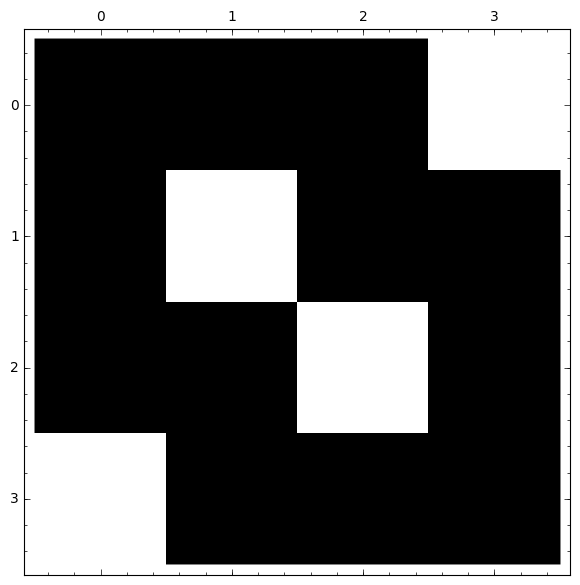
\includegraphics[width=.9\linewidth]{c2_1_weight_class_matrix.png}
  \captionof{figure}{$[f_{2,1}]$: weight classes. ~~~~\\~~~~}
  \label{fig:c2_1_weight_class_matrix}
\end{minipage}%
~~~~
\begin{minipage}{.48\textwidth}
  \centering
  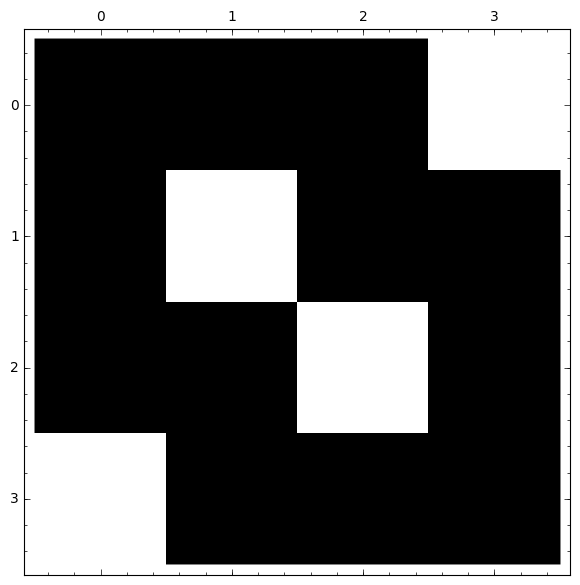
\includegraphics[width=.9\linewidth]{c2_1_bent_cayley_graph_index_matrix.png}
  \captionof{figure}{$[f_{2,1}]$: extended Cayley classes.}
  \label{fig:c2_1_bent_cayley_graph_index_matrix}
\end{minipage}
\end{figure}
As expected from Theorem~\ref{th-Quadratic-Classes},
the two extended Cayley classes correspond to the two weight classes,
as shown in Figures~\ref{fig:c2_1_weight_class_matrix} and~\ref{fig:c2_1_bent_cayley_graph_index_matrix}.

% \end{frame}
% \begin{frame}
\subsection{Bent functions in 4 dimensions}
%
The bent functions on $\F_2^4$ consist of one EA class, containing the ET class $[f_{4,1}]$ where
$f_{4,1}(x) := x_0 x_1 + x_2 x_3$ is self dual.
The ET class contains two extended Cayley classes as per Table~\ref{tab-c4_1_EC_classes}.
\begin{table}[!bhpt] % [H]
\small{
\begin{align*}
\def\arraystretch{1.2}
\begin{array}{|cccl|}
\hline
\text{Class} &
\text{Parameters} &
\text{2-rank} &
\text{Clique polynomial}
\\
\hline
0 &
(16, 6, 2, 2) &
6 &
\begin{array}{l}
8t^{4} + 32t^{3} + 48t^{2} + 16t + 1
\end{array}
\\
1 &
(16, 10, 6, 6) &
6 &
\begin{array}{l}
16t^{5} + 120t^{4} + 160t^{3}
\,+
\\
 80t^{2} + 16t + 1
\end{array}
\\
\hline
\end{array}
\end{align*}
}
\caption{$[f_{4,1}]$ extended Cayley classes.}
\label{tab-c4_1_EC_classes}
\end{table}

% The Cayley graphs for classes 1 and 2 are isomorphic to those those obtained from the
% projective two-weight codes listed in Table~\ref{tab-c4_1_codes}
%
% \begin{table}[!bhpt] % [H]
% \begin{align*}
% \begin{array}{|ccc|}
% \hline
% \text{Class} &
% \text{Parameters} & \text{Generator matrix}
% \\
% \hline
% 1 &
% [6, 4, 2] &
% \left[
% \begin{array}{cccccc}
% 0 & 0 & 1 & 1 & 1 & 1
% \\
% 1 & 0 & 0 & 1 & 1 & 1
% \\
% 1 & 1 & 1 & 1 & 0 & 0
% \\
% 0 & 1 & 1 & 1 & 1 & 0
% \end{array}
% \right]
% \\
% 2 &
% [5, 4, 2] &
% \left[
% \begin{array}{ccccc}
% 1 & 1 & 0 & 0 & 0
% \\
% 0 & 1 & 1 & 0 & 0
% \\
% 0 & 0 & 0 & 1 & 1
% \\
% 1 & 0 & 0 & 0 & 1
% \end{array}
% \right]
% \\
% \hline
% \end{array}
% \end{align*}
% \caption{$f_{4,1}$ Two-weight projective codes}
% \label{tab-c4_1_codes}
% \end{table}

\begin{figure}[!bhpt] % [H]
\centering
\begin{minipage}{.48\textwidth}
  \centering
  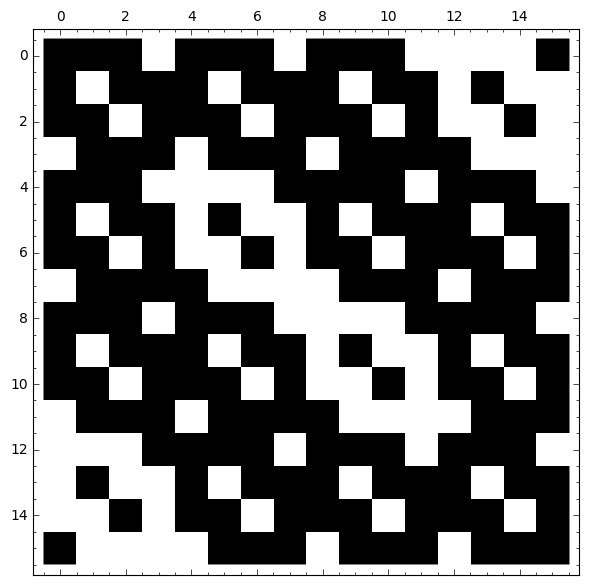
\includegraphics[width=.9\linewidth]{c4_1_weight_class_matrix.png}
  \captionof{figure}{$[f_{4,1}]$: weight classes. ~~~~\\~~~~}
  \label{fig:c4_1_weight_class_matrix}
\end{minipage}%
~~~~
\begin{minipage}{.48\textwidth}
  \centering
  \includegraphics[width=.9\linewidth]{c4_1_bent_cayley_graph_index_matrix.png}
  \captionof{figure}{$[f_{4,1}]$: extended Cayley classes.}
  \label{fig:c4_1_bent_cayley_graph_index_matrix}
\end{minipage}
\end{figure}
The two extended Cayley classes correspond to the two weight classes,
as shown in Figures~\ref{fig:c4_1_weight_class_matrix} and~\ref{fig:c4_1_bent_cayley_graph_index_matrix}.

% \end{frame}
\newpage
% \begin{frame}
\subsection{Bent functions in 6 dimensions}
\paragraph*{Extended affine classes.}
%
The bent functions on $\F_2^6$ consist of four
EA classes, containing the ET classes as listed in Table~\ref{tab-c6_ET_classes}
\cite[p. 303]{Rot76} \cite[Section 7.2]{Tok15bent}.
\begin{table}[!bhpt] % [H]
\small{
\begin{align*}
\def\arraystretch{1.2}
\begin{array}{|cl|}
\hline
\text{Class} &
\text{Representative}
\\
\hline
\,[f_{6,1}] & f_{6,1} :=
\begin{array}{l}
x_{0} x_{1} + x_{2} x_{3} + x_{4} x_{5}
\end{array}
\\
\,[f_{6,2}] & f_{6,2} :=
\begin{array}{l}
x_{0} x_{1} x_{2} + x_{0} x_{3} + x_{1} x_{4} + x_{2} x_{5}
\end{array}
\\
\,[f_{6,3}] & f_{6,3} :=
\begin{array}{l}
x_{0} x_{1} x_{2} + x_{0} x_{1} + x_{0} x_{3} + x_{1} x_{3} x_{4} + x_{1} x_{5}\, +
\\
x_{2} x_{4} + x_{3} x_{4}
\end{array}
\\
\,[f_{6,4}] & f_{6,4} :=
\begin{array}{l}
x_{0} x_{1} x_{2} + x_{0} x_{3} + x_{1} x_{3} x_{4} + x_{1} x_{5} + x_{2} x_{3} x_{5}\, +
\\
x_{2} x_{3} + x_{2} x_{4} + x_{2} x_{5} + x_{3} x_{4} + x_{3} x_{5}
\end{array}
\\
\hline
\end{array}
\end{align*}
}
\caption{6 dimensions: ET classes.}
\label{tab-c6_ET_classes}
\end{table}

%\newpage
In 1996, Tonchev classified the binary projective two-weight $[27,21,3]$ and $[35,6,16]$ codes
listing them in Tables 1 and 2, respectively, of his paper \cite{Ton96uniformly}.
These tables are repeated as Tables 1.155 and 1.156 in Chapter VII.1 of the Handbook of
Combinatorial Designs, Second Edition \cite{Ton07codes},
with a different numbering.
For each of the codes listed in these two tables, the characteristics of the corresponding
strongly regular graph is also listed.

In the classification given below, the Cayley graph of each Cayley class is matched by isomorphism
with a strongly regular graph corresponding to one
or more of Tonchev's projective two-weight codes, or the complement of such a graph.
Tonchev's strongly regular graphs were checked using the function
\verb!strongly_regular_from_two_weight_code!, which uses the smaller of the two weights to create the graph
\cite{SageMath7517}.
% \end{frame}
% \begin{frame}
%
\paragraph*{ET class $[f_{6,1}]$.}
%
This is the ET class of the bent function
$f_{6,1}(x) := x_0 x_1 + x_2 x_3 + x_4 x_5.$
This function is quadratic and self-dual.

The ET class contains two extended Cayley classes as per Table~\ref{tab-c6_1_EC_classes}.

\begin{table}[!bhpt] % [H]
%
\small{}
\begin{align*}
\def\arraystretch{1.2}
\begin{array}{|cccl|}
\hline
\text{Class} &
\text{Parameters} &
\text{2-rank} &
\text{Clique polynomial}
\\
\hline
0 &
(64, 28, 12, 12) &
8 &
\begin{array}{l}
64t^{8} + 512t^{7} + 1792t^{6} + 3584t^{5}
\,+
\\
 5376t^{4} + 3584t^{3} + 896t^{2} + 64t + 1
\end{array}
\\
1 &
(64, 36, 20, 20) &
8 &
\begin{array}{l}
2304t^{6} + 13824t^{5} + 19200t^{4} + 7680t^{3}
\,+
\\
 1152t^{2} + 64t + 1
\end{array}
\\
\hline
\end{array}
\end{align*}
%
\caption{$[f_{6,1}]$ extended Cayley classes.}
\label{tab-c6_1_EC_classes}
\end{table}

The Cayley graphs for classes 0 and 1 are isomorphic to those those obtained from the
Tonchev's projective two-weight codes \cite{Ton07codes} as per Table~\ref{tab-c6_1_codes}.

\begin{table}[!bhpt] % [H]
\small{
\begin{align*}
\def\arraystretch{1.2}
\begin{array}{|ccl|}
\hline
\text{Class} &
\text{Parameters} & \text{Reference}
\\
\hline
0 & [35,6,16] & \text{Table 1.156 1, 2 (complement)}
\\
1 & [27,6,12] & \text{Table 1.155 1 }
\\
\hline
\end{array}
\end{align*}
}
\caption{$[f_{6,1}]$ Two-weight projective codes.}
\label{tab-c6_1_codes}
\end{table}

%\slidecite{Tonchev 1996, 2006}
% \end{frame}
% \begin{frame}

The two extended Cayley classes correspond to the two weight classes,
as shown in Figures~\ref{fig:c6_1_weight_class_matrix} and~\ref{fig:c6_1_bent_cayley_graph_index_matrix}.

\begin{figure}[!bhpt] % [H]
\centering
\begin{minipage}{.48\textwidth}
  \centering
  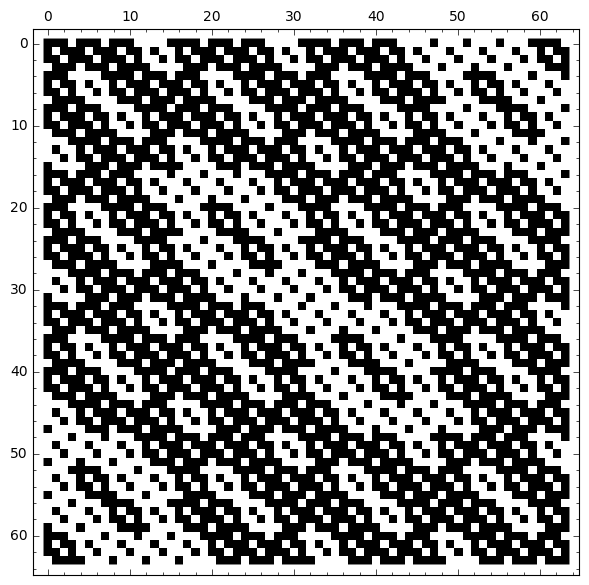
\includegraphics[width=.9\linewidth]{c6_1_weight_class_matrix.png}
  \captionof{figure}{$[f_{6,1}]$: weight classes. ~~~~\\~~~~}
  \label{fig:c6_1_weight_class_matrix}
\end{minipage}%
~~~~
\begin{minipage}{.48\textwidth}
  \centering
  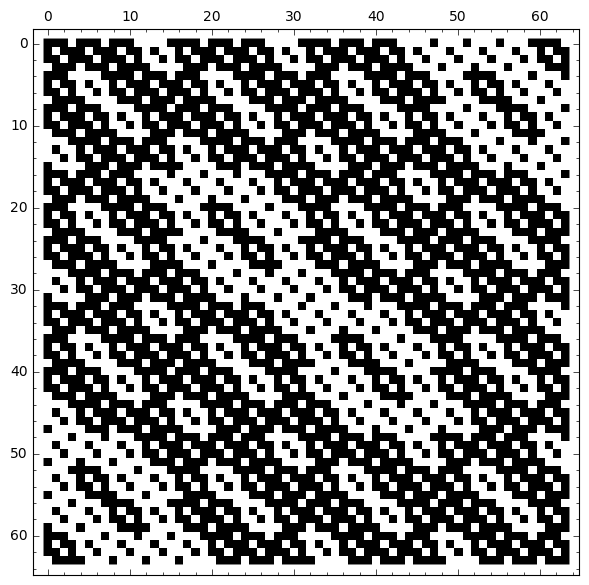
\includegraphics[width=.9\linewidth]{c6_1_bent_cayley_graph_index_matrix.png}
  \captionof{figure}{$[f_{6,1}]$: extended Cayley classes.}
  \label{fig:c6_1_bent_cayley_graph_index_matrix}
\end{minipage}
\end{figure}
%\newpage
Remark: The sequence of Figures~\ref{fig:c2_1_weight_class_matrix}, \ref{fig:c4_1_weight_class_matrix},
and \ref{fig:c6_1_weight_class_matrix} displays a fractal-like self-similar quality.

\paragraph*{ET class $[f_{6,2}]$.}
%
This is the ET class of the bent function
$f_{6,2}(x) := x_{0} x_{1} x_{2} + x_{0} x_{3} + x_{1} x_{4} + x_{2} x_{5}$.

The ET class contains three extended Cayley classes as per Table~\ref{tab-c6_2_EC_classes}.

\begin{table}[!bhpt] % [H]
%
\small{}
\begin{align*}
\def\arraystretch{1.2}
\begin{array}{|cccl|}
\hline
\text{Class} &
\text{Parameters} &
\text{2-rank} &
\text{Clique polynomial}
\\
\hline
0 &
(64, 28, 12, 12) &
8 &
\begin{array}{l}
64t^{8} + 512t^{7} + 1792t^{6} + 3584t^{5}
\,+
\\
 5376t^{4} + 3584t^{3} + 896t^{2} + 64t + 1
\end{array}
\\
1 &
(64, 28, 12, 12) &
8 &
\begin{array}{l}
256t^{6} + 1536t^{5} + 4352t^{4} + 3584t^{3}
\,+
\\
 896t^{2} + 64t + 1
\end{array}
\\
2 &
(64, 36, 20, 20) &
8 &
\begin{array}{l}
192t^{8} + 1536t^{7} + 8960t^{6} + 19968t^{5}
\,+
\\
 20224t^{4} + 7680t^{3} + 1152t^{2} + 64t + 1
\end{array}
\\
\hline
\end{array}
\end{align*}
%
\caption{$[f_{6,2}]$ extended Cayley classes.}
\label{tab-c6_2_EC_classes}
\end{table}

The Cayley graph for class 0 is isomorphic to graph 0 of ET class $[f_{6,1}]$,
This reflects the fact that $f_{6,1} \equiv f_{6,2}$, even though these two functions are not
EA equivalent.
This is therefore an example of an isomorphism between Cayley graphs of bent functions on
$\F_2^6$ that is not a linear function.

The Cayley graph for class 0 is also isomorphic to the complement of Royle's $(64,35,18,20)$ strongly regular graph $X$
\cite{Roy08normal}.

%
%~
%
%\slidecite{Royle 2008}
% \end{frame}
% \begin{frame}
%\paragraph*{ET class $[f_{6,2}]$: two-weight codes.}

The Cayley graphs for classes 0 to 2 are isomorphic to those those obtained from the
Tonchev's projective two-weight codes \cite{Ton07codes} as per Table~\ref{tab-c6_2_codes}.

\begin{table}[!bhpt] % [H]
\small{
\begin{align*}
\def\arraystretch{1.2}
\begin{array}{|ccl|}
\hline
\text{Class} &
\text{Parameters} & \text{Reference}
\\
\hline
0 & [35,6,16] & \text{Table 1.156 1, 2 (complement)}
\\
1 & [35,6,16] & \text{Table 1.156 3 (complement)}
\\
2 & [27,6,12] & \text{Table 1.155 2 }
\\
\hline
\end{array}
\end{align*}
}
\caption{$[f_{6,2}]$ Two-weight projective codes.}
\label{tab-c6_2_codes}
\end{table}
%\newpage

The three extended Cayley classes are distributed between the two weight classes,
as shown in Figures~\ref{fig:c6_2_weight_class_matrix} and~\ref{fig:c6_2_bent_cayley_graph_index_matrix}.

\begin{figure}[!bhpt] % [H]
\centering
\begin{minipage}{.48\textwidth}
  \centering
  \includegraphics[width=.9\linewidth]{c6_2_weight_class_matrix.png}
  \captionof{figure}{$[f_{6,2}]$: weight classes. ~~~~\\~~~~}
  \label{fig:c6_2_weight_class_matrix}
\end{minipage}%
~~~~
\begin{minipage}{.48\textwidth}
  \centering
  \includegraphics[width=.9\linewidth]{c6_2_bent_cayley_graph_index_matrix.png}
  \captionof{figure}{$[f_{6,2}]$: extended Cayley classes.}
  \label{fig:c6_2_bent_cayley_graph_index_matrix}
\end{minipage}
\end{figure}

%\slidecite{Tonchev 1996, 2006}
% \end{frame}
%%\newpage
% \begin{frame}
%
\paragraph*{ET class $[f_{6,3}]$.}
%
This is the ET class of the bent function
\begin{align*}
f_{6,3}(x) &= x_{0} x_{1} x_{2} + x_{0} x_{1} + x_{0} x_{3} + x_{1} x_{3} x_{4}
\\
           &+ x_{1} x_{5} + x_{2} x_{4} + x_{3} x_{4}.
\end{align*}

The ET class contains four extended Cayley classes as per Table~\ref{tab-c6_3_EC_classes}.

\begin{table}[!bhpt] % [H]
%
\small{}
\begin{align*}
\def\arraystretch{1.2}
\begin{array}{|cccl|}
\hline
\text{Class} &
\text{Parameters} &
\text{2-rank} &
\text{Clique polynomial}
\\
\hline
0 &
(64, 28, 12, 12) &
12 &
\begin{array}{l}
32t^{8} + 256t^{7} + 896t^{6} + 2048t^{5} + 4608t^{4}
\,+
\\
 3584t^{3} + 896t^{2} + 64t + 1
\end{array}
\\
1 &
(64, 36, 20, 20) &
12 &
\begin{array}{l}
160t^{8} + 1280t^{7} + 9344t^{6} + 21504t^{5}
\,+
\\
 20480t^{4} + 7680t^{3} + 1152t^{2} + 64t + 1
\end{array}
\\
2 &
(64, 28, 12, 12) &
12 &
\begin{array}{l}
64t^{6} + 1024t^{5} + 4096t^{4} + 3584t^{3}
\,+
\\
 896t^{2} + 64t + 1
\end{array}
\\
3 &
(64, 36, 20, 20) &
12 &
\begin{array}{l}
160t^{8} + 1664t^{7} + 9792t^{6} + 21504t^{5}
\,+
\\
 20480t^{4} + 7680t^{3} + 1152t^{2} + 64t + 1
\end{array}
\\
\hline
\end{array}
\end{align*}
%
\caption{$[f_{6,3}]$ extended Cayley classes.}
\label{tab-c6_3_EC_classes}
\end{table}

The Cayley graphs for classes 0 to 3 are isomorphic to those those obtained from the
Tonchev's projective two-weight codes \cite{Ton07codes} as per Table~\ref{tab-c6_3_codes}.

\begin{table}[!bhpt] % [H]
\small{
\begin{align*}
\def\arraystretch{1.2}
\begin{array}{|ccl|}
\hline
\text{Class} &
\text{Parameters} & \text{Reference}
\\
\hline
0 & [35,6,16] & \text{Table 1.156 4 (complement)}
\\
1 & [27,6,12] & \text{Table 1.155 3 }
\\
2 & [35,6,16] & \text{Table 1.156 5 (complement)}
\\
3 & [27,6,12] & \text{Table 1.155 4 }
\\
\hline
\end{array}
\end{align*}
}
\caption{$[f_{6,3}]$ Two-weight projective codes.}
\label{tab-c6_3_codes}
\end{table}

The four extended Cayley classes are distributed between the two weight classes,
as shown in Figures~\ref{fig:c6_3_weight_class_matrix} and~\ref{fig:c6_3_bent_cayley_graph_index_matrix}.

\begin{figure}[!ht] % [H]
\centering
\begin{minipage}{.48\textwidth}
  \centering
  \includegraphics[width=.9\linewidth]{c6_3_weight_class_matrix.png}
  \captionof{figure}{$[f_{6,3}]$: weight classes. ~~~~\\~~~~}
  \label{fig:c6_3_weight_class_matrix}
\end{minipage}%
~~~~
\begin{minipage}{.48\textwidth}
  \centering
  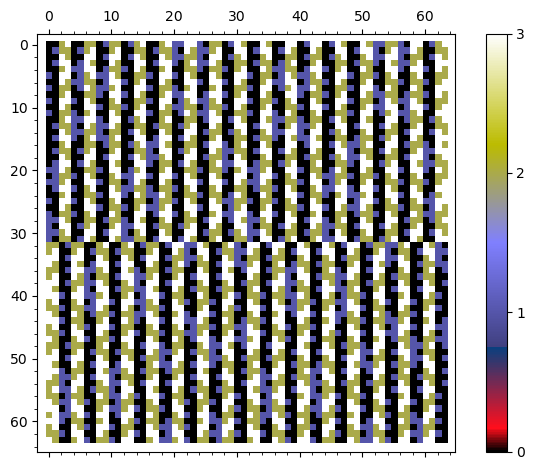
\includegraphics[width=.9\linewidth]{c6_3_bent_cayley_graph_index_matrix.png}
  \captionof{figure}{$[f_{6,3}]$: extended Cayley classes.}
  \label{fig:c6_3_bent_cayley_graph_index_matrix}
\end{minipage}
\end{figure}

%\slidecite{Tonchev 1996, 2006}
% \end{frame}
% \begin{frame}
%\newpage
\paragraph*{ET class $[f_{6,4}]$.}
%
This is the ET class of the bent function
\begin{align*}
f_{6,4}(x) &= x_{0} x_{1} x_{2} + x_{0} x_{3} + x_{1} x_{3} x_{4} + x_{1} x_{5} + x_{2} x_{3} x_{5}
\\
           &+ x_{2} x_{3} + x_{2} x_{4} + x_{2} x_{5} + x_{3} x_{4} + x_{3} x_{5}.
\end{align*}

The ET class contains three extended Cayley classes as per Table~\ref{tab-c6_4_EC_classes}.

\begin{table}[!bhpt] % [H]
%
\small{}
\begin{align*}
\def\arraystretch{1.2}
\begin{array}{|cccl|}
\hline
\text{Class} &
\text{Parameters} &
\text{2-rank} &
\text{Clique polynomial}
\\
\hline
0 &
(64, 28, 12, 12) &
14 &
\begin{array}{l}
32t^{8} + 256t^{7} + 896t^{6} + 1792t^{5} + 4480t^{4}
\,+
\\
 3584t^{3} + 896t^{2} + 64t + 1
\end{array}
\\
1 &
(64, 28, 12, 12) &
14 &
\begin{array}{l}
16t^{8} + 128t^{7} + 448t^{6} + 1280t^{5} + 4224t^{4}
\,+
\\
 3584t^{3} + 896t^{2} + 64t + 1
\end{array}
\\
2 &
(64, 36, 20, 20) &
14 &
\begin{array}{l}
176t^{8} + 1408t^{7} + 9664t^{6} + 22272t^{5}
\,+
\\
 20608t^{4} + 7680t^{3} + 1152t^{2} + 64t + 1
\end{array}
\\
\hline
\end{array}
\end{align*}
\caption{$[f_{6,4}]$ extended Cayley classes.}
\label{tab-c6_4_EC_classes}
\end{table}

The Cayley graphs for classes 0 to 2 are isomorphic to those those obtained from the
Tonchev's projective two-weight codes \cite{Ton07codes} as per Table~\ref{tab-c6_4_codes}.

\begin{table}[!bhpt] % [H]
\small{
\begin{align*}
\def\arraystretch{1.2}
\begin{array}{|ccl|}
\hline
\text{Class} &
\text{Parameters} & \text{Reference}
\\
\hline
0 & [35,6,16] & \text{Table 1.156 7 (complement)}
\\
1 & [35,6,16] & \text{Table 1.156 6 (complement)}
\\
2 & [27,6,12] & \text{Table 1.155 5 }
\\
\hline
\end{array}
\end{align*}
}
\caption{$[f_{6,4}]$ Two-weight projective codes.}
\label{tab-c6_4_codes}
\end{table}

%\slidecite{Tonchev 1996, 2006}
% \end{frame}
% \begin{frame}

The three extended Cayley classes are distributed between the two weight classes,
as shown in Figures~\ref{fig:c6_4_weight_class_matrix} and~\ref{fig:c6_4_bent_cayley_graph_index_matrix}.

\begin{figure}[!hpt] % [H]
\centering
\begin{minipage}{.48\textwidth}
  \centering
  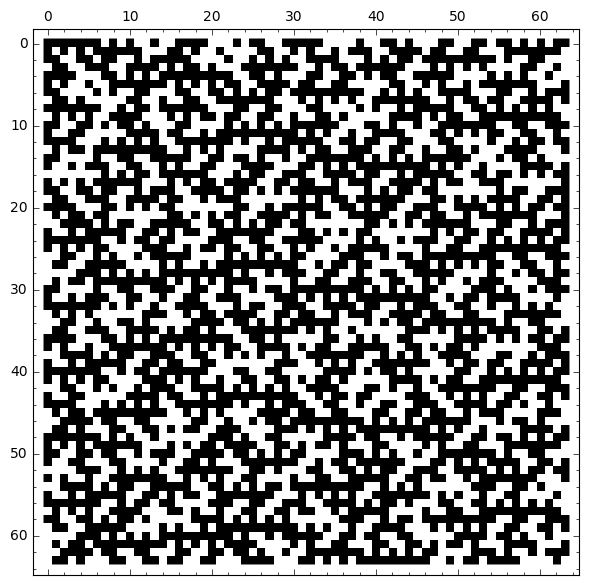
\includegraphics[width=.9\linewidth]{c6_4_weight_class_matrix.png}
  \captionof{figure}{$[f_{6,4}]$: weight classes. ~~~~\\~~~~}
  \label{fig:c6_4_weight_class_matrix}
\end{minipage}%
~~~~
\begin{minipage}{.48\textwidth}
  \centering
  \includegraphics[width=.9\linewidth]{c6_4_bent_cayley_graph_index_matrix.png}
  \captionof{figure}{$[f_{6,4}]$: extended Cayley classes.}
  \label{fig:c6_4_bent_cayley_graph_index_matrix}
\end{minipage}
\end{figure}
\newpage
\subsection{Bent functions in 8 dimensions}

There are
$99\,270\,589\,265\,934\,370\,305\,785\,861\,242\,880 \approx 2^{106}$ bent functions in 8 dimensions,
according to Langevin and Leander \cite{LanL11counting}.
%
%~
%
The number of EA classes has not yet been published,
let alone a list of representative bent functions.
The lists of EA classes of bent functions that have so far been published include those
for the bent functions of degree at most 3 \cite[Section 5.5.2]{Bra06thesis} \cite[Section 7.3]{Tok15bent},
and the partial spread bent functions \cite{Lan10psf,LanH11counting}.
The bent functions used in the S-boxes of the CAST-128 encryption algorithm \cite{Ada97,RFC2144}
are also representatives of disjoint EA classes.
%\newpage
\paragraph*{Extended affine classes of degree at most 3.}
%
According to a list contained in Braeken's PhD thesis \cite[Section 5.5.2]{Bra06thesis},
and repeated in Tokareva's table \cite[Section 7.3]{Tok15bent},
the bent functions on $\F_2^8$, of degree at most 3, consist of 10
EA classes, whose representatives are listed in Table~\ref{tab-c8_ET_classes}.
\begin{table}[!bhpt] % [H]
\small{}
\begin{align*}
\def\arraystretch{1.2}
\begin{array}{|cl|}
\hline
\text{Class} &
\text{Representative}
\\
\hline
\,[f_{ 8 , 1 }] & f_{ 8 , 1 } :=
\begin{array}{l}
x_{0} x_{1} + x_{2} x_{3} + x_{4} x_{5} + x_{6} x_{7}
\end{array}
\\
\,[f_{ 8 , 2 }] & f_{ 8 , 2 } :=
\begin{array}{l}
x_{0} x_{1} x_{2} + x_{0} x_{3} + x_{1} x_{4} + x_{2} x_{5} + x_{6} x_{7}
\end{array}
\\
\,[f_{ 8 , 3 }] & f_{ 8 , 3 } :=
\begin{array}{l}
x_{0} x_{1} x_{2} + x_{0} x_{6} + x_{1} x_{3} x_{4} + x_{1} x_{5} + x_{2} x_{3} + x_{4} x_{7}
\end{array}
\\
\,[f_{ 8 , 4 }] & f_{ 8 , 4 } :=
\begin{array}{l}
x_{0} x_{1} x_{2} + x_{0} x_{2} + x_{0} x_{4} + x_{1} x_{3} x_{4} + x_{1} x_{5} + x_{2} x_{3}\, +
x_{6} x_{7}
\end{array}
\\
\,[f_{ 8 , 5 }] & f_{ 8 , 5 } :=
\begin{array}{l}
x_{0} x_{1} x_{2} + x_{0} x_{6} + x_{1} x_{3} x_{4} + x_{1} x_{4} + x_{1} x_{5} + x_{2} x_{3} x_{5}
+ x_{2} x_{4} + x_{3} x_{7}
\end{array}
\\
\,[f_{ 8 , 6 }] & f_{ 8 , 6 } :=
\begin{array}{l}
x_{0} x_{1} x_{2} + x_{0} x_{2} + x_{0} x_{3} + x_{1} x_{3} x_{4} + x_{1} x_{6} + x_{2} x_{3} x_{5}
+ x_{2} x_{4} + x_{5} x_{7}
\end{array}
\\
\,[f_{ 8 , 7 }] & f_{ 8 , 7 } :=
\begin{array}{l}
x_{0} x_{1} x_{2} + x_{0} x_{1} + x_{0} x_{2} + x_{0} x_{3} + x_{1} x_{3} x_{4} + x_{1} x_{4}\, +
x_{1} x_{5}\, +
\\
x_{2} x_{3} x_{5} + x_{2} x_{4} + x_{6} x_{7}
\end{array}
\\
\,[f_{ 8 , 8 }] & f_{ 8 , 8 } :=
\begin{array}{l}
x_{0} x_{1} x_{2} + x_{0} x_{5} + x_{1} x_{3} x_{4} + x_{1} x_{6} + x_{2} x_{3} x_{5} + x_{2} x_{4}
+ x_{3} x_{7}
\end{array}
\\
\,[f_{ 8 , 9 }] & f_{ 8 , 9 } :=
\begin{array}{l}
x_{0} x_{1} x_{6} + x_{0} x_{3} + x_{1} x_{4} + x_{2} x_{3} x_{6} + x_{2} x_{5} + x_{3} x_{4}\, +
x_{4} x_{5} x_{6} + x_{6} x_{7}
\end{array}
\\
\,[f_{ 8 , 10 }] & f_{ 8 , 10 } :=
\begin{array}{l}
x_{0} x_{1} x_{2} + x_{0} x_{3} x_{6} + x_{0} x_{4} + x_{0} x_{5} + x_{1} x_{3} x_{4} + x_{1} x_{6}
+ x_{2} x_{3} x_{5}\, +
\\
x_{2} x_{4} + x_{3} x_{7}
\end{array}
\\
\hline
\end{array}
\end{align*}
\normalsize{}
\caption{8 dimensions to degree 3: ET classes.}
\label{tab-c8_ET_classes}
\end{table}
% \end{frame}
We here examine the corresponding ET classes in detail.
% \begin{frame}
\newpage
\paragraph*{ET class $[f_{8,1}]$.}
%
This is the ET class of the bent function
\small{}
\begin{align*}
f_{ 8 , 1 } &=
\begin{array}{l}
x_{0} x_{1} + x_{2} x_{3} + x_{4} x_{5} + x_{6} x_{7}.
\end{array}
\end{align*}
\normalsize{}
This function is quadratic and self-dual.
The ET class contains two extended Cayley classes as per Table~\ref{tab-c8_1_EC_classes}.

% f8_1
\begin{table}[!bhpt] % [H]
%
\small{}
\begin{align*}
\def\arraystretch{1.2}
\begin{array}{|cccl|}
\hline
\text{Class} &
\text{Parameters} &
\text{2-rank} &
\text{Clique polynomial}
\\
\hline
0 &
(256, 120, 56, 56) &
10 &
\begin{array}{l}
245760t^{9} + 3317760t^{8} + 8847360t^{7}
\,+
\\
 10321920t^{6} + 6193152t^{5} + 2007040t^{4}
\,+
\\
 286720t^{3} + 15360t^{2} + 256t + 1
\end{array}
\\
1 &
(256, 136, 72, 72) &
10 &
\begin{array}{l}
417792t^{8} + 3342336t^{7} + 11698176t^{6}
\,+
\\
 11698176t^{5} + 3760128t^{4} + 417792t^{3}
\,+
\\
 17408t^{2} + 256t + 1
\end{array}
\\
\hline
\end{array}
\end{align*}
%
\caption{$[f_{8,1}]$ extended Cayley classes.}
\label{tab-c8_1_EC_classes}
\end{table}

As expected from Theorem~\ref{th-Quadratic-Classes},
the two extended Cayley classes correspond to the two weight classes,
as shown in Figures~\ref{fig:c8_1_weight_class_matrix} and~\ref{fig:c8_1_bent_cayley_graph_index_matrix}.

Remark: The fractal-like self-similar quality of Figures~\ref{fig:c2_1_weight_class_matrix}, \ref{fig:c4_1_weight_class_matrix},
and \ref{fig:c6_1_weight_class_matrix} continues with Figure~\ref{fig:c8_1_weight_class_matrix}.

\begin{figure}[!bhpt] % [H]
\centering
\begin{minipage}{.48\textwidth}
  \centering
  \includegraphics[width=.9\linewidth]{c8_1_weight_class_matrix.png}
  \captionof{figure}{$[f_{8,1}]$: weight classes. ~~~~\\~~~~}
  \label{fig:c8_1_weight_class_matrix}
\end{minipage}%
~~~~
\begin{minipage}{.48\textwidth}
  \centering
  \includegraphics[width=.9\linewidth]{c8_1_bent_cayley_graph_index_matrix.png}
  \captionof{figure}{$[f_{8,1}]$: extended Cayley classes.}
  \label{fig:c8_1_bent_cayley_graph_index_matrix}
\end{minipage}
\end{figure}

% \end{frame}
% \begin{frame}
%
\paragraph*{ET class $[f_{8,2}]$.}
%
This is the ET class of the bent function
\small{}
\begin{align*}
f_{ 8 , 2 } &=
\begin{array}{l}
x_{0} x_{1} x_{2} + x_{0} x_{3} + x_{1} x_{4} + x_{2} x_{5} + x_{6} x_{7}.
\end{array}
\end{align*}
\normalsize{}
The ET class contains four extended Cayley classes as per Table~\ref{tab-c8_2_EC_classes}.

% f8_2
\begin{table}[!bhpt] % [H]
% f_{8,2}:
\small{}
\begin{align*}
\def\arraystretch{1.2}
\begin{array}{|cccl|}
\hline
\text{Class} &
\text{Parameters} &
\text{2-rank} &
\text{Clique polynomial}
\\
\hline
0 &
(256, 120, 56, 56) &
10 &
\begin{array}{l}
245760t^{9} + 3317760t^{8} + 8847360t^{7}
\,+
\\
 10321920t^{6} + 6193152t^{5} + 2007040t^{4}
\,+
\\
 286720t^{3} + 15360t^{2} + 256t + 1
\end{array}
\\
1 &
(256, 120, 56, 56) &
10 &
\begin{array}{l}
49152t^{9} + 663552t^{8} + 2555904t^{7}
\,+
\\
 5079040t^{6} + 4620288t^{5} + 1875968t^{4}
\,+
\\
 286720t^{3} + 15360t^{2} + 256t + 1
\end{array}
\\
2 &
(256, 136, 72, 72) &
10 &
\begin{array}{l}
327680t^{9} + 4055040t^{8} + 13828096t^{7}
\,+
\\
 22183936t^{6} + 14319616t^{5} + 3891200t^{4}
\,+
\\
 417792t^{3} + 17408t^{2} + 256t + 1
\end{array}
\\
3 &
(256, 136, 72, 72) &
10 &
\begin{array}{l}
417792t^{8} + 3342336t^{7} + 11698176t^{6}
\,+
\\
 11698176t^{5} + 3760128t^{4} + 417792t^{3}
\,+
\\
 17408t^{2} + 256t + 1
\end{array}
\\
\hline
\end{array}
\end{align*}
\caption{$[f_{8,2}]$ extended Cayley classes.}
\label{tab-c8_2_EC_classes}
\end{table}
%\newpage

\begin{figure}[!ht] % [H]
\centering
\begin{minipage}{.48\textwidth}
  \centering
  \includegraphics[width=.9\linewidth]{c8_2_weight_class_matrix.png}
  \captionof{figure}{$[f_{8,2}]$: weight classes. ~~~~\\~~~~}
  \label{fig:c8_2_weight_class_matrix}
\end{minipage}%
~~~~
\begin{minipage}{.48\textwidth}
  \centering
  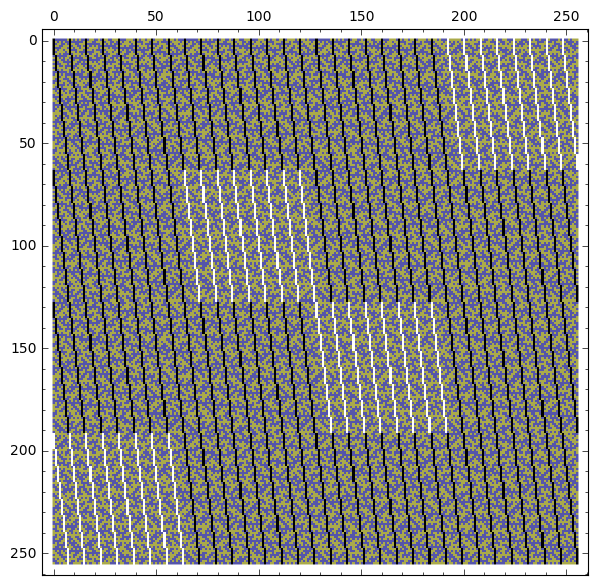
\includegraphics[width=.9\linewidth]{c8_2_bent_cayley_graph_index_matrix.png}
  \captionof{figure}{$[f_{8,2}]$: extended Cayley classes.}
  \label{fig:c8_2_bent_cayley_graph_index_matrix}
\end{minipage}
\end{figure}
~
% \end{frame}
\newpage
The Cayley graph for class 0 is isomorphic to graph 0 of ET class $[f_{8,1}]$,
This reflects the fact that $f_{8,1} \equiv f_{8,2}$, even though these two functions are not
EA equivalent.
This is therefore an example of an isomorphism between Cayley graphs of bent functions on
$\F_2^8$ that is not a linear function.

The four extended Cayley classes are distributed between the two weight classes,
as shown in Figures~\ref{fig:c8_2_weight_class_matrix} and~\ref{fig:c8_2_bent_cayley_graph_index_matrix}.

%\newpage
% \begin{frame}
%
\paragraph*{ET class $[f_{8,3}]$.}
%
This is the ET class of the bent function
\small{}
\begin{align*}
f_{ 8 , 3 } &=
\begin{array}{l}
x_{0} x_{1} x_{2} + x_{0} x_{6} + x_{1} x_{3} x_{4} + x_{1} x_{5} + x_{2} x_{3} + x_{4} x_{7}.
\end{array}
\end{align*}
\normalsize{}
The ET class contains six extended Cayley classes as per Table~\ref{tab-c8_3_EC_classes}.

% f8_3
\begin{table}[!bhpt] % [H]
%
% f_{8,3}:
\small{}
\begin{align*}
\def\arraystretch{1.2}
\begin{array}{|cccl|}
\hline
\text{Class} &
\text{Parameters} &
\text{2-rank} &
\text{Clique polynomial}
\\
\hline
0 &
(256, 120, 56, 56) &
12 &
\begin{array}{l}
81920t^{9} + 1368064t^{8} + 4653056t^{7}
\,+
\\
 7176192t^{6} + 5406720t^{5} + 1941504t^{4}
\,+
\\
 286720t^{3} + 15360t^{2} + 256t + 1
\end{array}
\\
1 &
(256, 136, 72, 72) &
12 &
\begin{array}{l}
294912t^{9} + 6299648t^{8} + 21692416t^{7}
\,+
\\
 27951104t^{6} + 15630336t^{5} + 3956736t^{4}
\,+
\\
 417792t^{3} + 17408t^{2} + 256t + 1
\end{array}
\\
2 &
(256, 120, 56, 56) &
12 &
\begin{array}{l}
16384t^{9} + 221184t^{8} + 1277952t^{7}
\,+
\\
 3768320t^{6} + 4227072t^{5} + 1843200t^{4}
\,+
\\
 286720t^{3} + 15360t^{2} + 256t + 1
\end{array}
\\
3 &
(256, 136, 72, 72) &
12 &
\begin{array}{l}
262144t^{9} + 4399104t^{8} + 16220160t^{7}
\,+
\\
 24281088t^{6} + 14974976t^{5} + 3923968t^{4}
\,+
\\
 417792t^{3} + 17408t^{2} + 256t + 1
\end{array}
\\
4 &
(256, 120, 56, 56) &
12 &
\begin{array}{l}
49152t^{9} + 729088t^{8} + 2686976t^{7}
\,+
\\
 5079040t^{6} + 4620288t^{5} + 1875968t^{4}
\,+
\\
 286720t^{3} + 15360t^{2} + 256t + 1
\end{array}
\\
5 &
(256, 136, 72, 72) &
12 &
\begin{array}{l}
196608t^{9} + 3399680t^{8} + 13172736t^{7}
\,+
\\
 21659648t^{6} + 14319616t^{5} + 3891200t^{4}
\,+
\\
 417792t^{3} + 17408t^{2} + 256t + 1
\end{array}
\\
\hline
\end{array}
\end{align*}
%
\caption{$[f_{8,3}]$ extended Cayley classes.}
\label{tab-c8_3_EC_classes}
\end{table}

The six extended Cayley classes are distributed between the two weight classes,
as shown in Figures~\ref{fig:c8_3_weight_class_matrix} and~\ref{fig:c8_3_bent_cayley_graph_index_matrix}.

\begin{figure}[!bhpt] % [H]
\centering
\begin{minipage}{.48\textwidth}
  \centering
  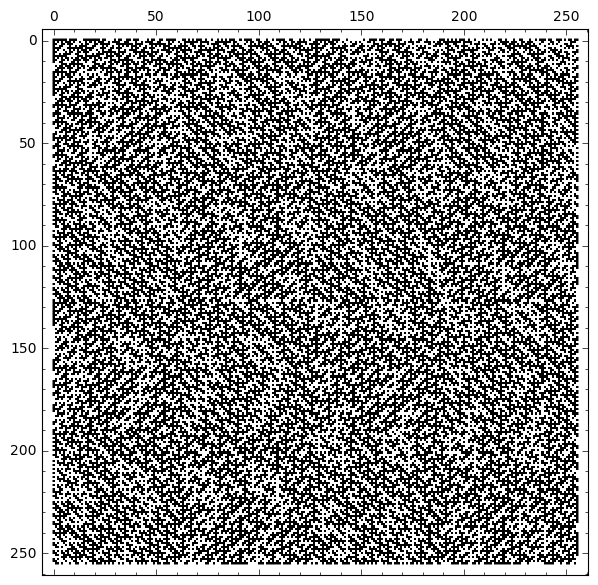
\includegraphics[width=.9\linewidth]{c8_3_weight_class_matrix.png}
  \captionof{figure}{$[f_{8,3}]$: weight classes. ~~~~\\~~~~}
  \label{fig:c8_3_weight_class_matrix}
\end{minipage}%
~~~~
\begin{minipage}{.48\textwidth}
  \centering
  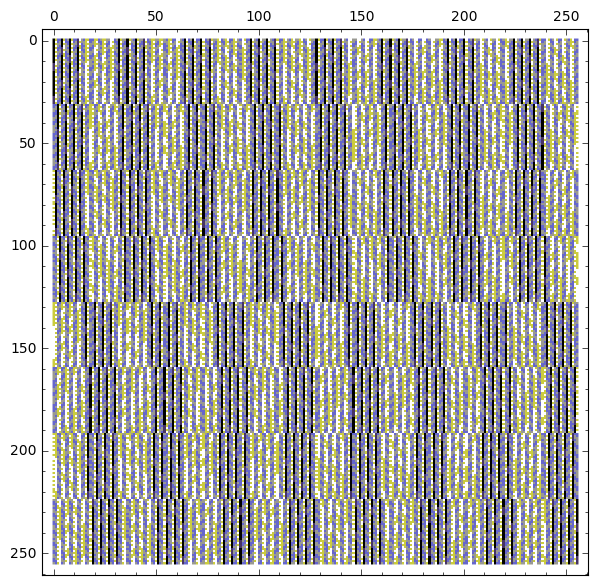
\includegraphics[width=.9\linewidth]{c8_3_bent_cayley_graph_index_matrix.png}
  \captionof{figure}{$[f_{8,3}]$: extended Cayley classes.}
  \label{fig:c8_3_bent_cayley_graph_index_matrix}
\end{minipage}
\end{figure}
~
% \end{frame}
\newpage
% \begin{frame}
%
\paragraph*{ET class $[f_{8,4}]$.}
This is the ET class of the bent function
\small{}
\begin{align*}
f_{ 8 , 4 } &=
\begin{array}{l}
x_{0} x_{1} x_{2} + x_{0} x_{2} + x_{0} x_{4} + x_{1} x_{3} x_{4} + x_{1} x_{5} + x_{2} x_{3}\, +
x_{6} x_{7}.
\end{array}
\end{align*}
\normalsize{}
The ET class contains six extended Cayley classes as per Table~\ref{tab-c8_4_EC_classes}.

The six extended Cayley classes are distributed between the two weight classes,
as shown in Figures~\ref{fig:c8_4_weight_class_matrix} and~\ref{fig:c8_4_bent_cayley_graph_index_matrix}.

% f8_4
\begin{table}[!bhpt] % [H]
%
\small{}
\begin{align*}
\def\arraystretch{1.2}
\begin{array}{|cccl|}
\hline
\text{Class} &
\text{Parameters} &
\text{2-rank} &
\text{Clique polynomial}
\\
\hline
0 &
(256, 120, 56, 56) &
14 &
\begin{array}{l}
69632t^{9} + 1099776t^{8} + 3784704t^{7}
\,+
\\
 6160384t^{6} + 5013504t^{5} + 1908736t^{4}
\,+
\\
 286720t^{3} + 15360t^{2} + 256t + 1
\end{array}
\\
1 &
(256, 136, 72, 72) &
14 &
\begin{array}{l}
225280t^{9} + 4319232t^{8} + 16203776t^{7}
\,+
\\
 24313856t^{6} + 14974976t^{5} + 3923968t^{4}
\,+
\\
 417792t^{3} + 17408t^{2} + 256t + 1
\end{array}
\\
2 &
(256, 120, 56, 56) &
14 &
\begin{array}{l}
1536t^{10} + 15360t^{9} + 209920t^{8}
\,+
\\
 1280000t^{7} + 3751936t^{6} + 4227072t^{5}
\,+
\\
 1843200t^{4} + 286720t^{3} + 15360t^{2} + 256t + 1
\end{array}
\\
3 &
(256, 136, 72, 72) &
14 &
\begin{array}{l}
7680t^{10} + 230400t^{9} + 4228096t^{8}
\,+
\\
 16058368t^{7} + 24166400t^{6} + 14974976t^{5}
\,+
\\
 3923968t^{4} + 417792t^{3} + 17408t^{2} + 256t + 1
\end{array}
\\
4 &
(256, 136, 72, 72) &
14 &
\begin{array}{l}
110592t^{9} + 2344960t^{8} + 10305536t^{7}
\,+
\\
 18939904t^{6} + 13664256t^{5} + 3858432t^{4}
\,+
\\
 417792t^{3} + 17408t^{2} + 256t + 1
\end{array}
\\
5 &
(256, 120, 56, 56) &
14 &
\begin{array}{l}
20480t^{9} + 337920t^{8} + 1556480t^{7}
\,+
\\
 3932160t^{6} + 4227072t^{5} + 1843200t^{4}
\,+
\\
 286720t^{3} + 15360t^{2} + 256t + 1
\end{array}
\\
\hline
\end{array}
\end{align*}
\caption{$[f_{8,4]}$ extended Cayley classes.}
\label{tab-c8_4_EC_classes}
\end{table}

\begin{figure}[!bhpt] % [H]
\centering
\begin{minipage}{.48\textwidth}
  \centering
  \includegraphics[width=.9\linewidth]{c8_4_weight_class_matrix.png}
  \captionof{figure}{$[f_{8,4}]$: weight classes. ~~~~\\~~~~}
  \label{fig:c8_4_weight_class_matrix}
\end{minipage}%
~~~~
\begin{minipage}{.48\textwidth}
  \centering
  \includegraphics[width=.9\linewidth]{c8_4_bent_cayley_graph_index_matrix.png}
  \captionof{figure}{$[f_{8,4}]$: extended Cayley classes.}
  \label{fig:c8_4_bent_cayley_graph_index_matrix}
\end{minipage}
\end{figure}
~
% \end{frame}
%%\newpage
% \begin{frame}
\paragraph*{ET class $[f_{8,5}]$.}
%
This is the ET class of the bent function
\small{}
\begin{align*}
f_{ 8 , 5 } &=
\begin{array}{l}
x_{0} x_{1} x_{2} + x_{0} x_{6} + x_{1} x_{3} x_{4} + x_{1} x_{4} + x_{1} x_{5} + x_{2} x_{3} x_{5}
+ x_{2} x_{4} + x_{3} x_{7}.
\end{array}
\end{align*}
\normalsize{}
The ET class contains 9 extended Cayley classes as per
%Tables~\ref{tab-c8_5_EC_classes} and~\ref{tab-c8_5_EC_classes_2}.
Table~\ref{tab-c8_5_EC_classes}.

% f8_5
\begin{table}[!bhpt] % [H]
%
\small{}
\begin{align*}
\def\arraystretch{1.2}
\begin{array}{|cccl|}
\hline
\text{Class} &
\text{Parameters} &
\text{2-rank} &
\text{Clique polynomial}
\\
\hline
0 &
(256, 120, 56, 56) &
14 &
\begin{array}{l}
32768t^{9} + 731136t^{8} + 3096576t^{7}
\,+
\\
 5767168t^{6} + 5013504t^{5} + 1908736t^{4}
\,+
\\
 286720t^{3} + 15360t^{2} + 256t + 1
\end{array}
\\
1 &
(256, 120, 56, 56) &
14 &
\begin{array}{l}
28672t^{9} + 534528t^{8} + 2211840t^{7}
\,+
\\
 4718592t^{6} + 4620288t^{5} + 1875968t^{4}
\,+
\\
 286720t^{3} + 15360t^{2} + 256t + 1
\end{array}
\\
2 &
(256, 136, 72, 72) &
14 &
\begin{array}{l}
159744t^{9} + 4753408t^{8} + 19021824t^{7}
\,+
\\
 26804224t^{6} + 15630336t^{5} + 3956736t^{4}
\,+
\\
 417792t^{3} + 17408t^{2} + 256t + 1
\end{array}
\\
3 &
(256, 120, 56, 56) &
14 &
\begin{array}{l}
24576t^{9} + 526336t^{8} + 2342912t^{7}
\,+
\\
 4849664t^{6} + 4620288t^{5} + 1875968t^{4}
\,+
\\
 286720t^{3} + 15360t^{2} + 256t + 1
\end{array}
\\
4 &
(256, 136, 72, 72) &
14 &
\begin{array}{l}
90112t^{9} + 2795520t^{8} + 12402688t^{7}
\,+
\\
 21168128t^{6} + 14319616t^{5} + 3891200t^{4}
\,+
\\
 417792t^{3} + 17408t^{2} + 256t + 1
\end{array}
\\
% \hline
% \end{array}
% \end{align*}
% \caption{$[f_{8,5}]$ extended Cayley classes (part 1).}
% \label{tab-c8_5_EC_classes}
% \end{table}
% %\newpage
% \begin{table}[!bhpt] % [H]
% \small{}
% \begin{align*}
% \def\arraystretch{1.2}
% \begin{array}{|cccl|}
% \hline
% \text{Class} &
% \text{Parameters} &
% \text{2-rank} &
% \text{Clique polynomial}
% \\
% \hline
5 &
(256, 120, 56, 56) &
14 &
\begin{array}{l}
16384t^{9} + 284672t^{8} + 1392640t^{7}
\,+
\\
 3735552t^{6} + 4227072t^{5} + 1843200t^{4}
\,+
\\
 286720t^{3} + 15360t^{2} + 256t + 1
\end{array}
\\
6 &
(256, 136, 72, 72) &
14 &
\begin{array}{l}
131072t^{9} + 3577856t^{8} + 15319040t^{7}
\,+
\\
 23855104t^{6} + 14974976t^{5} + 3923968t^{4}
\,+
\\
 417792t^{3} + 17408t^{2} + 256t + 1
\end{array}
\\
7 &
(256, 120, 56, 56) &
14 &
\begin{array}{l}
1536t^{10} + 19456t^{9} + 279552t^{8}
\,+
\\
 1394688t^{7} + 3751936t^{6} + 4227072t^{5}
\,+
\\
 1843200t^{4} + 286720t^{3} + 15360t^{2} + 256t + 1
\end{array}
\\
8 &
(256, 136, 72, 72) &
14 &
\begin{array}{l}
5632t^{10} + 148480t^{9} + 3621888t^{8}
\,+
\\
 15206400t^{7} + 23773184t^{6} + 14974976t^{5}
\,+
\\
 3923968t^{4} + 417792t^{3} + 17408t^{2} + 256t + 1
\end{array}
\\
\hline
\end{array}
\end{align*}
%\caption{$[f_{8,5}]$ extended Cayley classes (part 2).}
\caption{$[f_{8,5}]$ extended Cayley classes.}
%\label{tab-c8_5_EC_classes_2}
\label{tab-c8_5_EC_classes}
\end{table}
\newpage
The 9 extended Cayley classes are distributed between the two weight classes,
as shown in Figures~\ref{fig:c8_5_weight_class_matrix} and~\ref{fig:c8_5_bent_cayley_graph_index_matrix}.

\begin{figure}[!bhpt] % [H]
\centering
\begin{minipage}{.48\textwidth}
  \centering
  \includegraphics[width=.9\linewidth]{c8_5_weight_class_matrix.png}
  \captionof{figure}{$[f_{8,5}]$: weight classes. ~~~~\\~~~~}
  \label{fig:c8_5_weight_class_matrix}
\end{minipage}%
~~~~
\begin{minipage}{.48\textwidth}
  \centering
  \includegraphics[width=.9\linewidth]{c8_5_bent_cayley_graph_index_matrix.png}
  \captionof{figure}{$[f_{8,5}]$: extended Cayley classes.}
  \label{fig:c8_5_bent_cayley_graph_index_matrix}
\end{minipage}
\end{figure}
~
% \end{frame}
%\newpage
% \begin{frame}
\paragraph*{ET class $[f_{8,6}]$.}
%
%
This is the ET class of the bent function
\small{}
\begin{align*}
f_{ 8 , 6 } &=
\begin{array}{l}
x_{0} x_{1} x_{2} + x_{0} x_{2} + x_{0} x_{3} + x_{1} x_{3} x_{4} + x_{1} x_{6} + x_{2} x_{3} x_{5}
+ x_{2} x_{4} + x_{5} x_{7}.
\end{array}
\end{align*}
\normalsize{}
The ET class contains 9 extended Cayley classes.
% as per
%Tables~\ref{tab-c8_6_EC_classes} and~\ref{tab-c8_6_EC_classes_2}.

%Each such isomorphism between
%the Cayley graph of a function in $[f_{8,5}]$ and
%the Cayley graph of a function in $[f_{8,6}]$ is not a linear function on $\F_2^8$.

%
% % f8_6
% \begin{table}[!bhpt] % [H]
% %
% \small{}
% \begin{align*}
% \def\arraystretch{1.2}
% \begin{array}{|cccl|}
% \hline
% \text{Class} &
% \text{Parameters} &
% \text{2-rank} &
% \text{Clique polynomial}
% \\
% \hline
% 0 &
% (256, 120, 56, 56) &
% 14 &
% \begin{array}{l}
% 32768t^{9} + 731136t^{8} + 3096576t^{7}
% \,+
% \\
%  5767168t^{6} + 5013504t^{5} + 1908736t^{4}
% \,+
% \\
%  286720t^{3} + 15360t^{2} + 256t + 1
% \end{array}
% \\
% 1 &
% (256, 120, 56, 56) &
% 14 &
% \begin{array}{l}
% 28672t^{9} + 534528t^{8} + 2211840t^{7}
% \,+
% \\
%  4718592t^{6} + 4620288t^{5} + 1875968t^{4}
% \,+
% \\
%  286720t^{3} + 15360t^{2} + 256t + 1
% \end{array}
% \\
% 2 &
% (256, 136, 72, 72) &
% 14 &
% \begin{array}{l}
% 159744t^{9} + 4753408t^{8} + 19021824t^{7}
% \,+
% \\
%  26804224t^{6} + 15630336t^{5} + 3956736t^{4}
% \,+
% \\
%  417792t^{3} + 17408t^{2} + 256t + 1
% \end{array}
% \\
% 3 &
% (256, 120, 56, 56) &
% 14 &
% \begin{array}{l}
% 1536t^{10} + 19456t^{9} + 279552t^{8}
% \,+
% \\
%  1394688t^{7} + 3751936t^{6} + 4227072t^{5}
% \,+
% \\
%  1843200t^{4} + 286720t^{3} + 15360t^{2} + 256t + 1
% \end{array}
% \\
% 4 &
% (256, 136, 72, 72) &
% 14 &
% \begin{array}{l}
% 5632t^{10} + 148480t^{9} + 3621888t^{8}
% \,+
% \\
%  15206400t^{7} + 23773184t^{6} + 14974976t^{5}
% \,+
% \\
%  3923968t^{4} + 417792t^{3} + 17408t^{2} + 256t + 1
% \end{array}
% \\
% \hline
% \end{array}
% \end{align*}
% \caption{$[f_{8,6}]$ extended Cayley classes (part 1).}
% \label{tab-c8_6_EC_classes}
% \end{table}
% %\newpage
% \begin{table}[!bhpt] % [H]
% \small{}
% \begin{align*}
% \def\arraystretch{1.2}
% \begin{array}{|cccl|}
% \hline
% \text{Class} &
% \text{Parameters} &
% \text{2-rank} &
% \text{Clique polynomial}
% \\
% \hline
% 5 &
% (256, 120, 56, 56) &
% 14 &
% \begin{array}{l}
% 24576t^{9} + 526336t^{8} + 2342912t^{7}
% \,+
% \\
%  4849664t^{6} + 4620288t^{5} + 1875968t^{4}
% \,+
% \\
%  286720t^{3} + 15360t^{2} + 256t + 1
% \end{array}
% \\
% 6 &
% (256, 120, 56, 56) &
% 14 &
% \begin{array}{l}
% 16384t^{9} + 284672t^{8} + 1392640t^{7}
% \,+
% \\
%  3735552t^{6} + 4227072t^{5} + 1843200t^{4}
% \,+
% \\
%  286720t^{3} + 15360t^{2} + 256t + 1
% \end{array}
% \\
% 7 &
% (256, 136, 72, 72) &
% 14 &
% \begin{array}{l}
% 131072t^{9} + 3577856t^{8} + 15319040t^{7}
% \,+
% \\
%  23855104t^{6} + 14974976t^{5} + 3923968t^{4}
% \,+
% \\
%  417792t^{3} + 17408t^{2} + 256t + 1
% \end{array}
% \\
% 8 &
% (256, 136, 72, 72) &
% 14 &
% \begin{array}{l}
% 90112t^{9} + 2795520t^{8} + 12402688t^{7}
% \,+
% \\
%  21168128t^{6} + 14319616t^{5} + 3891200t^{4}
% \,+
% \\
%  417792t^{3} + 17408t^{2} + 256t + 1
% \end{array}
% \\
% \hline
% \end{array}
% \end{align*}
% %
% \caption{$[f_{8,6}]$ extended Cayley classes (part 2).}
% %\caption{$[f_{8,6}]$ extended Cayley classes.}
% \label{tab-c8_6_EC_classes_2}
% %\label{tab-c8_6_EC_classes}
% \end{table}

\begin{figure}[!hb] % [H]
\centering
\begin{minipage}{.48\textwidth}
  \centering
  \includegraphics[width=.9\linewidth]{c8_6_weight_class_matrix.png}
  \captionof{figure}{$[f_{8,6}]$: weight classes. ~~~~\\~~~~}
  \label{fig:c8_6_weight_class_matrix}
\end{minipage}%
~~~~
\begin{minipage}{.48\textwidth}
  \centering
  \includegraphics[width=.9\linewidth]{c8_6_bent_cayley_graph_index_matrix.png}
  \captionof{figure}{$[f_{8,6}]$: extended Cayley classes.}
  \label{fig:c8_6_bent_cayley_graph_index_matrix}
\end{minipage}
\end{figure}
% \end{frame}

The 9 extended Cayley classes are distributed between the two weight classes,
as shown in Figures~\ref{fig:c8_6_weight_class_matrix} and~\ref{fig:c8_6_bent_cayley_graph_index_matrix}.

The 9 Cayley graphs corresponding to the 9 classes are isomorphic to those for the extended Cayley classes for $[f_{8,5}]$.
The corresponding Cayley classes have the same frequency within each of these two ET classes.
This correspondence is shown in Table~\ref{tab-c8_5-c8_6_EC_classes}.

Figures~\ref{fig:re8_5_bent_cayley_graph_index_matrix} and~\ref{fig:re8_5_bent_cayley_graph_index_matrix}
show the 9 extended Cayley classes of each of $[f_{8,5}]$ and $[f_{8,6}]$ with corresponding Cayley classes
given the same colour.

\begin{table}[!bhpt] % [H]
%
\small{}
\begin{align*}
\def\arraystretch{1.2}
\begin{array}{|ccr|}
\hline
[f_{8,5}] &
[f_{8,6}] &
\text{Frequency}
\\
\hline
  0 &    0 &  4096
\\
  1 &    1 &  6144
\\
  2 &    2 &  6144
\\
  3 &    5 &  2048
\\
  4 &    8 &  2048
\\
  5 &    6 &  6144
\\
  6 &    7 &  6144
\\
  7 &    3 & 16384
\\
  8 &    4 & 16384
\\
\hline
\end{array}
\end{align*}
\caption{Correspondence between $[f_{8,5}]$ and $[f_{8,6}]$ extended Cayley classes.}
\label{tab-c8_5-c8_6_EC_classes}
\end{table}

\begin{figure}[!bhpt] % [H]
\centering
\begin{minipage}{.48\textwidth}
  \centering
  \includegraphics[width=.9\linewidth]{re8_5_bent_cayley_graph_index_matrix.png}
  \captionof{figure}{$[f_{8,5}]$: extended Cayley classes (recoloured).}
  \label{fig:re8_5_bent_cayley_graph_index_matrix}
\end{minipage}
~~
\begin{minipage}{.48\textwidth}
  \centering
  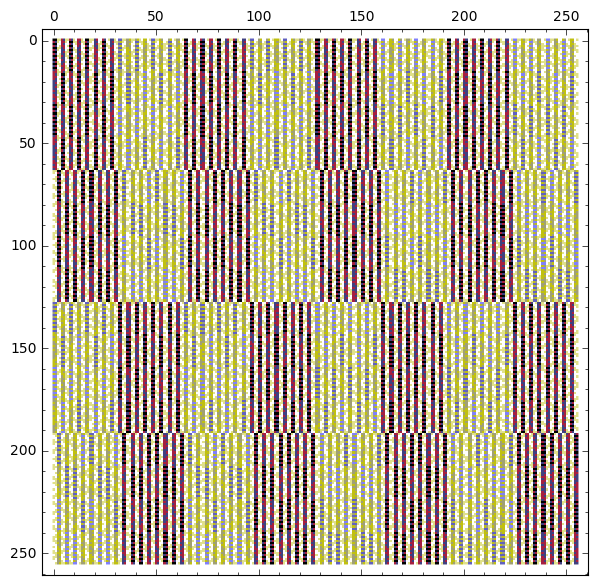
\includegraphics[width=.9\linewidth]{re8_6_bent_cayley_graph_index_matrix.png}
  \captionof{figure}{$[f_{8,6}]$: extended Cayley classes (recoloured).}
  \label{fig:re8_6_bent_cayley_graph_index_matrix}
\end{minipage}
\end{figure}
\newpage
The explanation for the correspondence between the Cayley classes of $f_{8,5}$ and $f_{8,6}$
is quite simple. The functions $f_{8,5}$ and $f_{8,6}$ are EA equivalent,
in fact general linear equivalent, and therefore Braeken's list of EA equivalence classes
\cite[Section 5.5.2]{Bra06thesis} contains an error.

\begin{Theorem}
\label{th-f8-5-f8-6-linearly-equiv}
Functions $f_{8,5}$ and $f_{8,6}$ are general linear equivalent.
\end{Theorem}

\begin{proof}

Apply the permutation $\pi := (x_0\ x_5\ x_4)(x_1\ x_2\ x_3)(x_6\ x_7)$ to
\small{
\begin{align*}
f_{8,5}
&=
x_{0} x_{1} x_{2} + x_{0} x_{6} + x_{1} x_{3} x_{4} + x_{1} x_{4} + x_{1} x_{5} + x_{2} x_{3} x_{5} + x_{2} x_{4} + x_{3} x_{7}
%\end{align*}
%}\normalsize{}
\intertext{\normalsize{to obtain}}
%\small{
%\begin{align*}
\pi(f_{8,5})
&=
x_{5} x_{2} x_{3} + x_{5} x_{7} + x_{2} x_{1} x_{0} + x_{2} x_{0} + x_{2} x_{4} + x_{3} x_{1} x_{4} + x_{3} x_{0} + x_{1} x_{6}
\\
&=
x_{0} x_{1} x_{2} + x_{0} x_{2} + x_{0} x_{3} + x_{1} x_{3} x_{4} + x_{1} x_{6} + x_{2} x_{3} x_{5} + x_{2} x_{4} + x_{5} x_{7}
\\
&= f_{8,6}.
\end{align*}
}\normalsize{}
\end{proof}

%\newpage
% \begin{frame}
\paragraph*{ET class $[f_{8,7}]$.}
%
This is the ET class of the bent function
\small{}
\begin{align*}
f_{ 8 , 7 } &=
\begin{array}{l}
x_{0} x_{1} x_{2} + x_{0} x_{1} + x_{0} x_{2} + x_{0} x_{3} + x_{1} x_{3} x_{4} + x_{1} x_{4}\, +
x_{1} x_{5}\, +
\\
x_{2} x_{3} x_{5} + x_{2} x_{4} + x_{6} x_{7}.
\end{array}
\end{align*}
\normalsize{}
The ET class contains six extended Cayley classes as per Table~\ref{tab-c8_7_EC_classes}.

The six extended Cayley classes are distributed between the two weight classes,
as shown in Figures~\ref{fig:c8_7_weight_class_matrix} and~\ref{fig:c8_7_bent_cayley_graph_index_matrix}.

% f8_7
\begin{table}[!bhpt] % [H]
\small{}
\begin{align*}
\def\arraystretch{1.2}
\begin{array}{|cccl|}
\hline
\text{Class} &
\text{Parameters} &
\text{2-rank} &
\text{Clique polynomial}
\\
\hline
0 &
(256, 120, 56, 56) &
16 &
\begin{array}{l}
29696t^{9} + 655360t^{8} + 2789376t^{7}
\,+
\\
 5332992t^{6} + 4816896t^{5} + 1892352t^{4}
\,+
\\
 286720t^{3} + 15360t^{2} + 256t + 1
\end{array}
\\
1 &
(256, 120, 56, 56) &
16 &
\begin{array}{l}
20480t^{9} + 409600t^{8} + 1837056t^{7}
\,+
\\
 4235264t^{6} + 4423680t^{5} + 1859584t^{4}
\,+
\\
 286720t^{3} + 15360t^{2} + 256t + 1
\end{array}
\\
2 &
(256, 136, 72, 72) &
16 &
\begin{array}{l}
143360t^{9} + 3981312t^{8} + 16697344t^{7}
\,+
\\
 25108480t^{6} + 15302656t^{5} + 3940352t^{4}
\,+
\\
 417792t^{3} + 17408t^{2} + 256t + 1
\end{array}
\\
3 &
(256, 136, 72, 72) &
16 &
\begin{array}{l}
64512t^{9} + 2316288t^{8} + 10932224t^{7}
\,+
\\
 19783680t^{6} + 13991936t^{5} + 3874816t^{4}
\,+
\\
 417792t^{3} + 17408t^{2} + 256t + 1
\end{array}
\\
4 &
(256, 136, 72, 72) &
16 &
\begin{array}{l}
92160t^{9} + 2979840t^{8} + 13608960t^{7}
\,+
\\
 22388736t^{6} + 14647296t^{5} + 3907584t^{4}
\,+
\\
 417792t^{3} + 17408t^{2} + 256t + 1
\end{array}
\\
5 &
(256, 120, 56, 56) &
16 &
\begin{array}{l}
6144t^{9} + 124928t^{8} + 944128t^{7}
\,+
\\
 3219456t^{6} + 4030464t^{5} + 1826816t^{4}
\,+
\\
 286720t^{3} + 15360t^{2} + 256t + 1
\end{array}
\\
\hline
\end{array}
\end{align*}

\caption{$[f_{8,7}]$ extended Cayley classes.}
\label{tab-c8_7_EC_classes}
\end{table}

\begin{figure}[!bhpt] % [H]
\centering
\begin{minipage}{.48\textwidth}
  \centering
  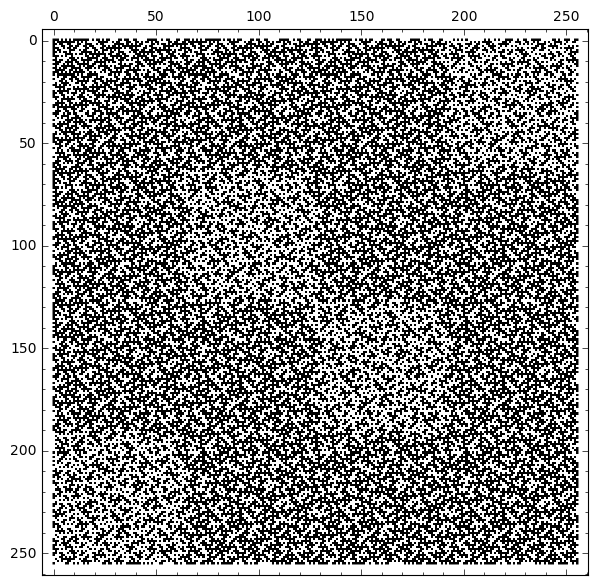
\includegraphics[width=.9\linewidth]{c8_7_weight_class_matrix.png}
  \captionof{figure}{$[f_{8,7}]$: weight classes. ~~~~\\~~~~}
  \label{fig:c8_7_weight_class_matrix}
\end{minipage}%
~~~~
\begin{minipage}{.48\textwidth}
  \centering
  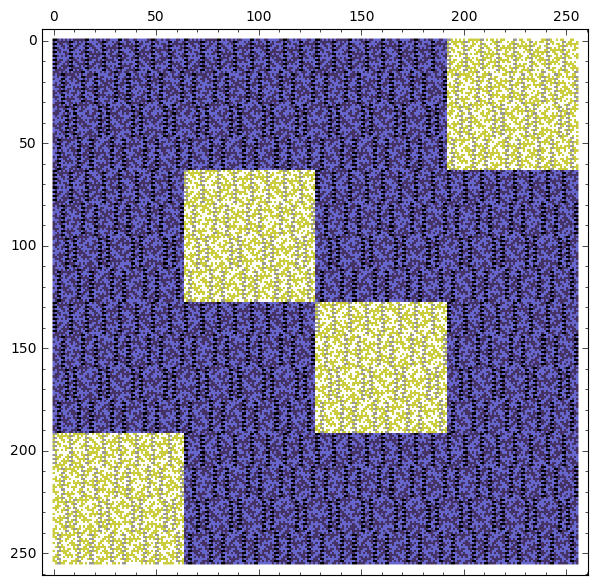
\includegraphics[width=.9\linewidth]{c8_7_bent_cayley_graph_index_matrix.png}
  \captionof{figure}{$[f_{8,7}]$: extended Cayley classes.}
  \label{fig:c8_7_bent_cayley_graph_index_matrix}
\end{minipage}
\end{figure}

% \end{frame}
\newpage
% \begin{frame}
\paragraph*{ET class $[f_{8,8}]$.}
%
This is the ET class of the bent function
\small{}
\begin{align*}
f_{ 8 , 8 } &=
\begin{array}{l}
x_{0} x_{1} x_{2} + x_{0} x_{5} + x_{1} x_{3} x_{4} + x_{1} x_{6} + x_{2} x_{3} x_{5} + x_{2} x_{4}
+ x_{3} x_{7}.
\end{array}
\end{align*}
\normalsize{}
The ET class contains six extended Cayley classes as per Table~\ref{tab-c8_8_EC_classes}.

The six extended Cayley classes are distributed between the two weight classes,
as shown in Figures~\ref{fig:c8_8_weight_class_matrix} and~\ref{fig:c8_8_bent_cayley_graph_index_matrix}.

% f8_8
\begin{table}[!bhpt] % [H]
\small{}
\begin{align*}
\def\arraystretch{1.2}
\begin{array}{|cccl|}
\hline
\text{Class} &
\text{Parameters} &
\text{2-rank} &
\text{Clique polynomial}
\\
\hline
0 &
(256, 120, 56, 56) &
14 &
\begin{array}{l}
32768t^{9} + 712704t^{8} + 3014656t^{7}
\,+
\\
 5734400t^{6} + 5013504t^{5} + 1908736t^{4}
\,+
\\
 286720t^{3} + 15360t^{2} + 256t + 1
\end{array}
\\
1 &
(256, 120, 56, 56) &
14 &
\begin{array}{l}
24576t^{9} + 466944t^{8} + 2064384t^{7}
\,+
\\
 4685824t^{6} + 4620288t^{5} + 1875968t^{4}
\,+
\\
 286720t^{3} + 15360t^{2} + 256t + 1
\end{array}
\\
2 &
(256, 136, 72, 72) &
14 &
\begin{array}{l}
172032t^{9} + 5332992t^{8} + 20283392t^{7}
\,+
\\
 27295744t^{6} + 15630336t^{5} + 3956736t^{4}
\,+
\\
 417792t^{3} + 17408t^{2} + 256t + 1
\end{array}
\\
3 &
(256, 136, 72, 72) &
14 &
\begin{array}{l}
147456t^{9} + 3858432t^{8} + 15990784t^{7}
\,+
\\
 24150016t^{6} + 14974976t^{5} + 3923968t^{4}
\,+
\\
 417792t^{3} + 17408t^{2} + 256t + 1
\end{array}
\\
4 &
(256, 120, 56, 56) &
14 &
\begin{array}{l}
16384t^{9} + 270336t^{8} + 1376256t^{7}
\,+
\\
 3768320t^{6} + 4227072t^{5} + 1843200t^{4}
\,+
\\
 286720t^{3} + 15360t^{2} + 256t + 1
\end{array}
\\
5 &
(256, 136, 72, 72) &
14 &
\begin{array}{l}
163840t^{9} + 3858432t^{8} + 15532032t^{7}
\,+
\\
 23887872t^{6} + 14974976t^{5} + 3923968t^{4}
\,+
\\
 417792t^{3} + 17408t^{2} + 256t + 1
\end{array}
\\
\hline
\end{array}
\end{align*}
\caption{$[f_{8,8}]$ extended Cayley classes.}
\label{tab-c8_8_EC_classes}
\end{table}

\begin{figure}[!bhpt] % [H]
\centering
\begin{minipage}{.48\textwidth}
  \centering
  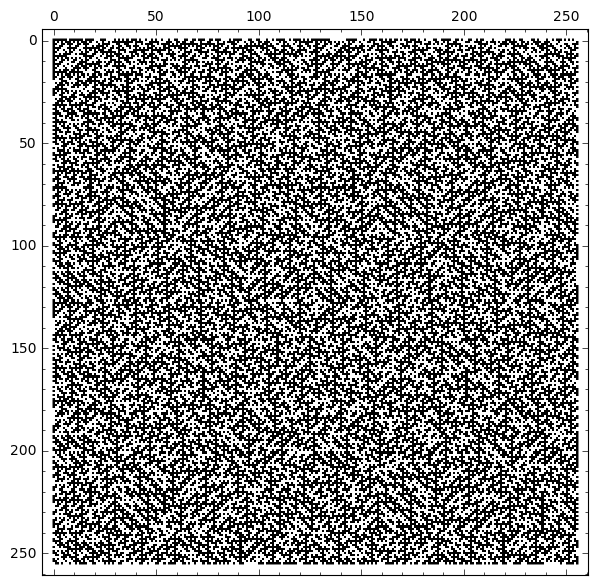
\includegraphics[width=.9\linewidth]{c8_8_weight_class_matrix.png}
  \captionof{figure}{$[f_{8,8}]$: weight classes. ~~~~\\~~~~}
  \label{fig:c8_8_weight_class_matrix}
\end{minipage}%
~~~~
\begin{minipage}{.48\textwidth}
  \centering
  \includegraphics[width=.9\linewidth]{c8_8_bent_cayley_graph_index_matrix.png}
  \captionof{figure}{$[f_{8,8}]$: extended Cayley classes.}
  \label{fig:c8_8_bent_cayley_graph_index_matrix}
\end{minipage}
\end{figure}

% \end{frame}
\newpage
% \begin{frame}
\paragraph*{ET class $[f_{8,9}]$.}
%
%
This is the ET class of the bent function
\small{}
\begin{align*}
f_{ 8 , 9 } &=
\begin{array}{l}
x_{0} x_{1} x_{6} + x_{0} x_{3} + x_{1} x_{4} + x_{2} x_{3} x_{6} + x_{2} x_{5} + x_{3} x_{4}\, +
x_{4} x_{5} x_{6} + x_{6} x_{7}.
\end{array}
\end{align*}
\normalsize{}
The ET class contains 8 extended Cayley classes as per
%Tables~\ref{tab-c8_9_EC_classes} and~\ref{tab-c8_9_EC_classes_2}.
Table~\ref{tab-c8_9_EC_classes}.
In 4 of these 8 classes, each bent function is extended Cayley equivalent to its dual.
In the remaining 4 extended Cayley classes, the dual of every bent function in the class has a Cayley graph
that is isomorphic to that of one other class. That is, the 4 Cayley classes form two duality pairs of classes.
This correspondence between Cayley classes and Cayley classes of duals is shown in Table~\ref{tab-c8_9-dual-EC_classes}.

\begin{figure}[!bhpt] % [H]
\centering
\begin{minipage}{.48\textwidth}
  \centering
  \includegraphics[width=.9\linewidth]{c8_9_bent_cayley_graph_index_matrix.png}
  \captionof{figure}{$[f_{8,9}]$: 8 extended Cayley classes ~~ ~~~~ ~~~~ ~~~~~~~~~}
  \label{fig:c8_9_bent_cayley_graph_index_matrix}
\end{minipage}
~~
\begin{minipage}{.48\textwidth}
  \centering
  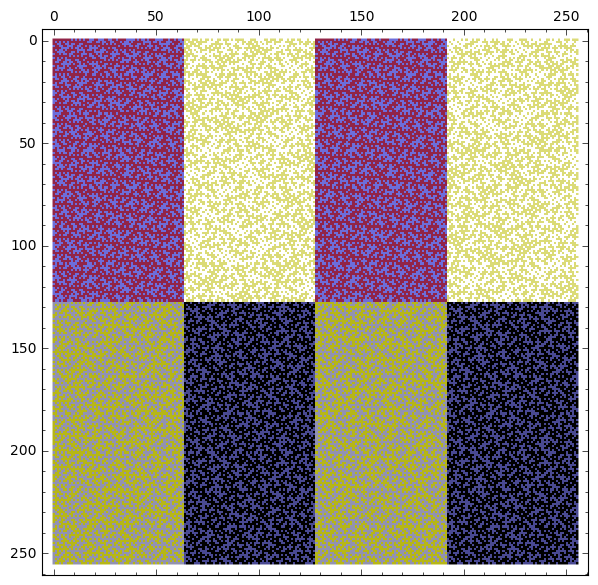
\includegraphics[width=.9\linewidth]{c8_9_dual_cayley_graph_index_matrix.png}
  \captionof{figure}{$[f_{8,9}]$: 8 extended Cayley classes of dual bent functions}
  \label{fig:c8_9_dual_cayley_graph_index_matrix}
\end{minipage}%
\end{figure}

The 8 extended Cayley classes are distributed
as shown in Figures~\ref{fig:c8_9_bent_cayley_graph_index_matrix} (classes) and~\ref{fig:c8_9_dual_cayley_graph_index_matrix}
(classes of duals).

% f8_9
\begin{table}[!bhpt] % [H]
\small{}
\begin{align*}
\def\arraystretch{1.2}
\begin{array}{|cccl|}
\hline
\text{Class} &
\text{Parameters} &
\text{2-rank} &
\text{Clique polynomial}
\\
\hline
0 &
(256, 120, 56, 56) &
16 &
\begin{array}{l}
45056t^{9} + 780288t^{8} + 2998272t^{7}
\,+
\\
 5505024t^{6} + 4816896t^{5} + 1892352t^{4}
\,+
\\
 286720t^{3} + 15360t^{2} + 256t + 1
\end{array}
\\
1 &
(256, 120, 56, 56) &
16 &
\begin{array}{l}
45056t^{9} + 780288t^{8} + 2998272t^{7}
\,+
\\
 5505024t^{6} + 4816896t^{5} + 1892352t^{4}
\,+
\\
 286720t^{3} + 15360t^{2} + 256t + 1
\end{array}
\\
2 &
(256, 136, 72, 72) &
16 &
\begin{array}{l}
184320t^{9} + 3852288t^{8} + 14893056t^{7}
\,+
\\
 23003136t^{6} + 14647296t^{5} + 3907584t^{4}
\,+
\\
 417792t^{3} + 17408t^{2} + 256t + 1
\end{array}
\\
3 &
(256, 136, 72, 72) &
16 &
\begin{array}{l}
184320t^{9} + 3852288t^{8} + 14893056t^{7}
\,+
\\
 23003136t^{6} + 14647296t^{5} + 3907584t^{4}
\,+
\\
 417792t^{3} + 17408t^{2} + 256t + 1
\end{array}
\\
4 &
(256, 120, 56, 56) &
16 &
\begin{array}{l}
105984t^{8} + 976896t^{7} + 3440640t^{6}
\,+
\\
 4128768t^{5} + 1835008t^{4} + 286720t^{3}
\,+
\\
 15360t^{2} + 256t + 1
\end{array}
\\
% \hline
% \end{array}
% \end{align*}
% \caption{$[f_{8,9}]$ extended Cayley classes (part 1).}
% \label{tab-c8_9_EC_classes}
% \end{table}
% %%\newpage
% \begin{table}[!bhpt] % [H]
% \small{}
% \begin{align*}
% \def\arraystretch{1.2}
% \begin{array}{|cccl|}
% \hline
% \text{Class} &
% \text{Parameters} &
% \text{2-rank} &
% \text{Clique polynomial}
% \\
% \hline
5 &
(256, 136, 72, 72) &
16 &
\begin{array}{l}
9216t^{10} + 264192t^{9} + 4468224t^{8}
\,+
\\
 16803840t^{7} + 24772608t^{6} + 15138816t^{5}
\,+
\\
 3932160t^{4} + 417792t^{3} + 17408t^{2} + 256t + 1
\end{array}
\\
6 &
(256, 120, 56, 56) &
16 &
\begin{array}{l}
9216t^{9} + 124416t^{8} + 976896t^{7}
\,+
\\
 3440640t^{6} + 4128768t^{5} + 1835008t^{4}
\,+
\\
 286720t^{3} + 15360t^{2} + 256t + 1
\end{array}
\\
7 &
(256, 136, 72, 72) &
16 &
\begin{array}{l}
193536t^{9} + 4449792t^{8} + 16803840t^{7}
\,+
\\
 24772608t^{6} + 15138816t^{5} + 3932160t^{4}
\,+
\\
 417792t^{3} + 17408t^{2} + 256t + 1
\end{array}
\\
\hline
\end{array}
\end{align*}
%\caption{$[f_{8,9}]$ extended Cayley classes (part 2).}
\caption{$[f_{8,9}]$ extended Cayley classes.}
%\label{tab-c8_9_EC_classes_2}
\label{tab-c8_9_EC_classes}
\end{table}

\begin{table}
\small{}
\begin{align*}
\def\arraystretch{1.2}
\begin{array}{|ccc|}
\hline
[f_{8,9}] &
[f_{8,9}] &
\text{Frequency}
\\
&
\text{duals} &
\\
\hline
0 &   1 & 9216
\\
1 &   0 & 9216
\\
2 &   3 & 7168
\\
3 &   2 & 7168
\\
4 &   4 & 8192
\\
5 &   5 & 8192
\\
6 &   6 & 8192
\\
7 &   7 & 8192
\\
\hline
\end{array}
\end{align*}
\caption{Correspondence between $[f_{8,9}]$ extended Cayley classes and $[f_{8,9}]$ dual extended Cayley classes.}
\label{tab-c8_9-dual-EC_classes}
\end{table}
% \end{frame}
\newpage
% \begin{frame}
\paragraph*{ET class $[f_{8,10}]$.}
%
This is the ET class of the bent function
\small{}
\begin{align*}
f_{ 8 , 10 } :=
\begin{array}{l}
x_{0} x_{1} x_{2} + x_{0} x_{3} x_{6} + x_{0} x_{4} + x_{0} x_{5} + x_{1} x_{3} x_{4} + x_{1} x_{6}
+ x_{2} x_{3} x_{5}\, +
\\
x_{2} x_{4} + x_{3} x_{7}.
\end{array}
\end{align*}
\normalsize{}
The ET class contains 10 extended Cayley classes as per
Table~\ref{tab-c8_10_EC_classes}.
%Tables~\ref{tab-c8_10_EC_classes} and~\ref{tab-c8_10_EC_classes_2}.
In 4 of these 10 classes, each bent function is extended Cayley equivalent to its dual.
In the remaining 6 extended Cayley classes, the dual of every bent function in the class has a Cayley graph
that is isomorphic to that of one other class. That is, the 6 Cayley classes form three duality pairs of classes.
This correspondence between Cayley classes and Cayley classes of duals is shown in Table~\ref{tab-c8_10-dual-EC_classes}.

The 10 extended Cayley classes are distributed
as shown in Figures~\ref{fig:c8_10_bent_cayley_graph_index_matrix} (classes) and~\ref{fig:c8_10_dual_cayley_graph_index_matrix}
(classes of duals).
% f8_10
\begin{table}[!bhpt] % [H]
\small{}
\begin{align*}
\def\arraystretch{1.2}
\begin{array}{|cccl|}
\hline
\text{Class} &
\text{Parameters} &
\text{2-rank} &
\text{Clique polynomial}
\\
\hline
0 &
(256, 120, 56, 56) &
16 &
\begin{array}{l}
16384t^{9} + 464896t^{8} + 2310144t^{7}
\,+
\\
 5046272t^{6} + 4816896t^{5} + 1892352t^{4}
\,+
\\
 286720t^{3} + 15360t^{2} + 256t + 1
\end{array}
\\
1 &
(256, 120, 56, 56) &
16 &
\begin{array}{l}
16384t^{9} + 464896t^{8} + 2310144t^{7}
\,+
\\
 5046272t^{6} + 4816896t^{5} + 1892352t^{4}
\,+
\\
 286720t^{3} + 15360t^{2} + 256t + 1
\end{array}
\\
2 &
(256, 120, 56, 56) &
16 &
\begin{array}{l}
12288t^{9} + 301056t^{8} + 1589248t^{7}
\,+
\\
 4128768t^{6} + 4423680t^{5} + 1859584t^{4}
\,+
\\
 286720t^{3} + 15360t^{2} + 256t + 1
\end{array}
\\
3 &
(256, 120, 56, 56) &
16 &
\begin{array}{l}
12288t^{9} + 301056t^{8} + 1589248t^{7}
\,+
\\
 4128768t^{6} + 4423680t^{5} + 1859584t^{4}
\,+
\\
 286720t^{3} + 15360t^{2} + 256t + 1
\end{array}
\\
4 &
(256, 136, 72, 72) &
16 &
\begin{array}{l}
110592t^{9} + 4159488t^{8} + 17285120t^{7}
\,+
\\
 25296896t^{6} + 15302656t^{5} + 3940352t^{4}
\,+
\\
 417792t^{3} + 17408t^{2} + 256t + 1
\end{array}
\\
% \hline
% \end{array}
% \end{align*}
% \caption{$[f_{8,10}]$ extended Cayley classes (part 1).}
% \label{tab-c8_10_EC_classes}
% \end{table}
% %%\newpage
% \begin{table}[!bhpt] % [H]
% \small{}
% \begin{align*}
% \def\arraystretch{1.2}
% \begin{array}{|cccl|}
% \hline
% \text{Class} &
% \text{Parameters} &
% \text{2-rank} &
% \text{Clique polynomial}
% \\
% \hline
5 &
(256, 136, 72, 72) &
16 &
\begin{array}{l}
110592t^{9} + 4159488t^{8} + 17285120t^{7}
\,+
\\
 25296896t^{6} + 15302656t^{5} + 3940352t^{4}
\,+
\\
 417792t^{3} + 17408t^{2} + 256t + 1
\end{array}
\\
6 &
(256, 120, 56, 56) &
16 &
\begin{array}{l}
2048t^{9} + 167424t^{8} + 1091584t^{7}
\,+
\\
 3440640t^{6} + 4128768t^{5} + 1835008t^{4}
\,+
\\
 286720t^{3} + 15360t^{2} + 256t + 1
\end{array}
\\
7 &
(256, 136, 72, 72) &
16 &
\begin{array}{l}
7168t^{10} + 143360t^{9} + 3804672t^{8}
\,+
\\
 15886336t^{7} + 24313856t^{6} + 15138816t^{5}
\,+
\\
 3932160t^{4} + 417792t^{3} + 17408t^{2} + 256t + 1
\end{array}
\\
8 &
(256, 120, 56, 56) &
16 &
\begin{array}{l}
9216t^{9} + 181760t^{8} + 1091584t^{7}
\,+
\\
 3440640t^{6} + 4128768t^{5} + 1835008t^{4}
\,+
\\
 286720t^{3} + 15360t^{2} + 256t + 1
\end{array}
\\
9 &
(256, 136, 72, 72) &
16 &
\begin{array}{l}
107520t^{9} + 3790336t^{8} + 15886336t^{7}
\,+
\\
 24313856t^{6} + 15138816t^{5} + 3932160t^{4}
\,+
\\
 417792t^{3} + 17408t^{2} + 256t + 1
\end{array}
\\
\hline
\end{array}
\end{align*}
%\caption{$[f_{8,10}]$ extended Cayley classes (part 2).}
\caption{$[f_{8,10}]$ extended Cayley classes.}
%\label{tab-c8_10_EC_classes_2}
\label{tab-c8_10_EC_classes}
\end{table}

\begin{table}
\small{}
\begin{align*}
\def\arraystretch{1.2}
\begin{array}{|ccc|}
\hline
[f_{8,10}] &
[f_{8,10}] &
\text{Frequency}
\\
&
\text{duals} &
\\
\hline
  0 &    1 & 2048
\\
  1 &    0 & 2048
\\
  2 &    3 & 7168
\\
  3 &    2 & 7168
\\
  4 &    5 & 7168
\\
  5 &    4 & 7168
\\
  6 &    6 & 8192
\\
  7 &    7 & 8192
\\
  8 &    8 & 8192
\\
  9 &    9 & 8192
\\
\hline
\end{array}
\end{align*}
\caption{Correspondence between $[f_{8,10}]$ extended Cayley classes and $[f_{8,10}]$ dual extended Cayley classes.}
\label{tab-c8_10-dual-EC_classes}
\end{table}

\begin{figure}[!bhpt] % [H]
\centering
\begin{minipage}{.48\textwidth}
  \centering
  \includegraphics[width=.9\linewidth]{c8_10_bent_cayley_graph_index_matrix.png}
  \captionof{figure}{$[f_{8,10}]$: extended Cayley classes.}
  \label{fig:c8_10_bent_cayley_graph_index_matrix}
\end{minipage}
~~
\begin{minipage}{.48\textwidth}
  \centering
  \includegraphics[width=.9\linewidth]{c8_10_dual_cayley_graph_index_matrix.png}
  \captionof{figure}{$[f_{8,10}]$: extended Cayley classes of dual bent functions.}
  \label{fig:c8_10_dual_cayley_graph_index_matrix}
\end{minipage}%
\end{figure}
% \end{frame}
% \end{colortheme}
% \begin{colortheme}{seagull}
% \begin{frame}
\newpage

\subsection{Two sequences of bent functions}

As stated in the introduction, in a recent paper \cite{Leo17Hurwitz},
the author found an example of two infinite series of bent functions whose
Cayley graphs have the same strongly regular parameters at each dimension,
but are not isomorphic if the dimension is 8 or more.
The sequences are $\sigma_m$ and $\tau_m$ for $m \geqslant 1$,
whose definitions are reproduced here from \cite{Leo15Twin}.

\begin{definition}
\label{def-sigma-tau}
The sign-of-square function $\sigma_m : \Z_2^{2 m} \To \Z_2$ is defined as follows:

For $i \in \Z_{2^{2m}},$ $\sigma_m(i) = 1$ if and only if the number of
1 digits in the base 4 representation of $i$ is odd.

The non-diagonal-symmetry function $\tau_m \mid \Z_{2^{2 m}} \To \Z_2$
is defined as follows.

For $i$ in $\Z_2^2$:
\begin{align*}
&\tau_1(i) :=
\begin{cases}
1 &\text{if~}i = 10,
\\
0 &\text{otherwise}.
\end{cases}
\end{align*}

For $i$ in $\Z_2^{2 m - 2}$:
\begin{align*}
&\tau_m (00 \odot i) := \tau_{m-1}(i),
\\
&\tau_m (01 \odot i) := \sigma_{m-1}(i),
\\
&\tau_m (10 \odot i) := \sigma_{m-1}(i) + 1,
\\
&\tau_m (11 \odot i) := \tau_{m-1}(i).
\end{align*}
where $\odot$ denotes concatenation of bit vectors, and $\sigma$ is the sign-of-square function, as above.
\end{definition}

As shown in  \cite{Leo15Twin}, both sequences produce Cayley graphs whose strongly regular parameters are
\begin{align*}
(v_m,k_m,\lambda_m=\mu_m) &= (4^m, 2^{2 m - 1} - 2^{m-1}, 2^{2 m - 2} - 2^{m-1}).
\end{align*}

%\begin{colortheme}{jubata}

%\begin{frame}
%\frametitle{For 2 dimensions: $[\sigma_1]$ and $[\tau_1]$}
\begin{figure}[!ht]
\centering
\begin{minipage}{.48\textwidth}
  \centering
  \includegraphics[width=.9\linewidth]{sigma_1_bent_cayley_graph_index_matrix.png}
  \captionof{figure}{$[\sigma_1]$:\\2 extended Cayley classes}
  \label{fig:sigma_1_bent_cayley_graph_index_matrix}
\end{minipage}%
\begin{minipage}{.48\textwidth}
  \centering
  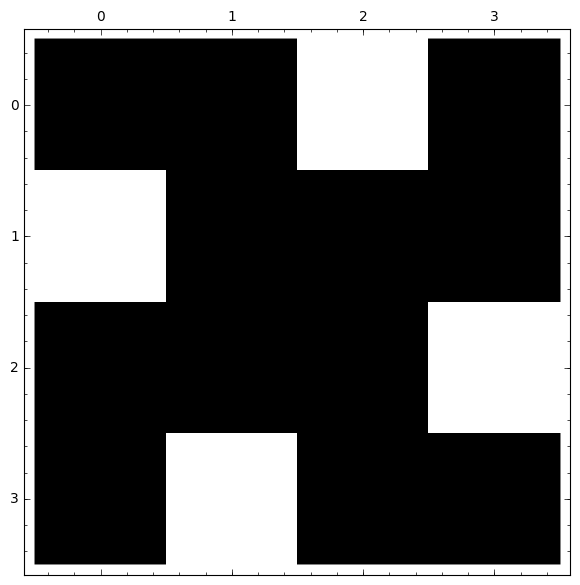
\includegraphics[width=.9\linewidth]{tau_1_bent_cayley_graph_index_matrix.png}
  \captionof{figure}{$[\tau_1]$:\\2 extended Cayley classes}
  \label{fig:tau_1_bent_cayley_graph_index_matrix}
\end{minipage}
\end{figure}
%\end{frame}

%\begin{frame}
%\frametitle{For 4 dimensions: $[\sigma_2]$ and $[\tau_2]$}
\begin{figure}[!hb]
\centering
\begin{minipage}{.48\textwidth}
  \centering
  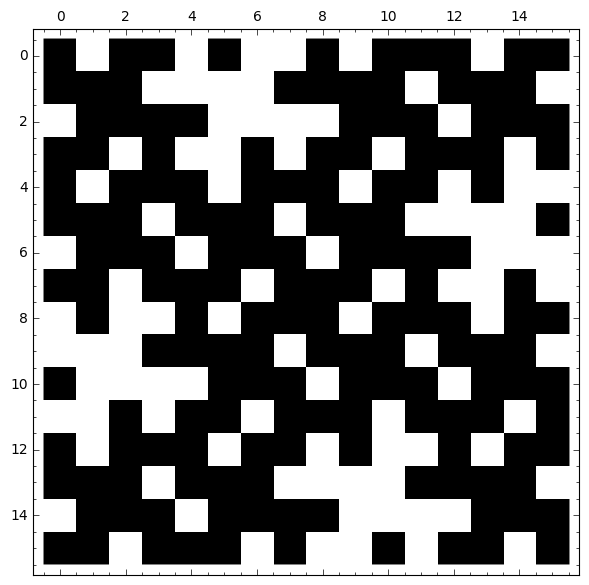
\includegraphics[width=.9\linewidth]{sigma_2_bent_cayley_graph_index_matrix.png}
  \captionof{figure}{$[\sigma_2]$:\\2 extended Cayley classes}
  \label{fig:sigma_2_bent_cayley_graph_index_matrix}
\end{minipage}%
\begin{minipage}{.48\textwidth}
  \centering
  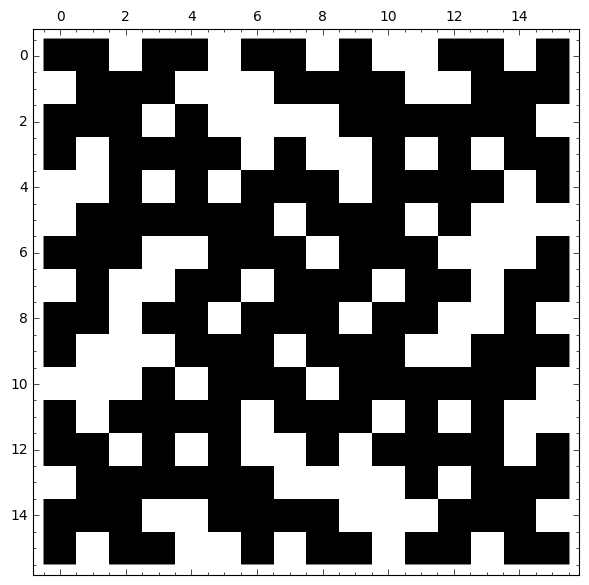
\includegraphics[width=.9\linewidth]{tau_2_bent_cayley_graph_index_matrix.png}
  \captionof{figure}{$[\tau_2]$:\\2 extended Cayley classes}
  \label{fig:tau_2_bent_cayley_graph_index_matrix}
\end{minipage}
\end{figure}
%\end{frame}

Figures \ref{fig:sigma_1_bent_cayley_graph_index_matrix} to \ref{fig:tau_4_bent_cayley_graph_index_matrix}
illustrate the extended Cayley classes within the ET classes of each of function $\sigma_m$ and $\tau_m$ for $m$ from 1 to 4.
Note that $\tau_3$ has degree 3, and $\tau_4$ has degree 4.
As shown in \cite{Leo17Hurwitz},
The functions $\sigma_m$ and $\tau_m$ are extended Cayley equivalent for $m$ from 1 to 3, but are inequivalent for $m>3$.

%\begin{frame}
%\frametitle{For 6 dimensions: $[\sigma_3]$ and $[\tau_3]$}
\begin{figure}[!ht]
\centering
\begin{minipage}{.48\textwidth}
  \centering
  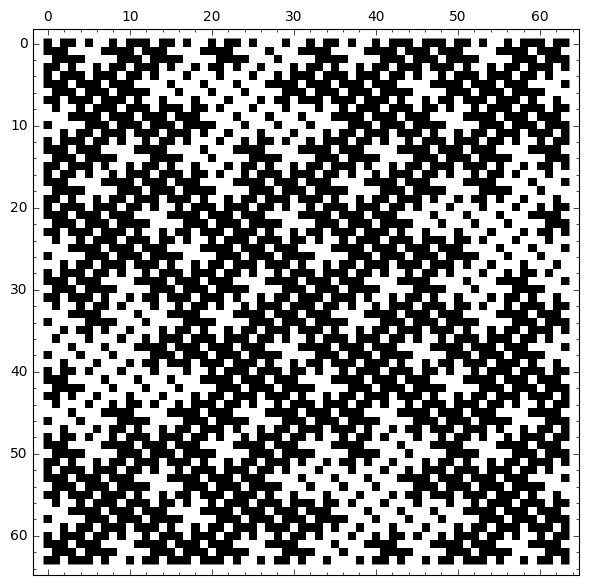
\includegraphics[width=.9\linewidth]{sigma_3_bent_cayley_graph_index_matrix.png}
  \captionof{figure}{$[\sigma_3]$:\\2 extended Cayley classes}
  \label{fig:sigma_3_bent_cayley_graph_index_matrix}
\end{minipage}%
\begin{minipage}{.48\textwidth}
  \centering
  \includegraphics[width=.9\linewidth]{tau_3_bent_cayley_graph_index_matrix.png}
  \captionof{figure}{$[\tau_3]$:\\3 extended Cayley classes}
  \label{fig:tau_3_bent_cayley_graph_index_matrix}
\end{minipage}
\end{figure}
%\end{frame}

%\begin{frame}
%\frametitle{For 8 dimensions: $[\sigma_4]$ and $[\tau_4]$}
\begin{figure}[!hb]
\centering
\begin{minipage}{.48\textwidth}
  \centering
  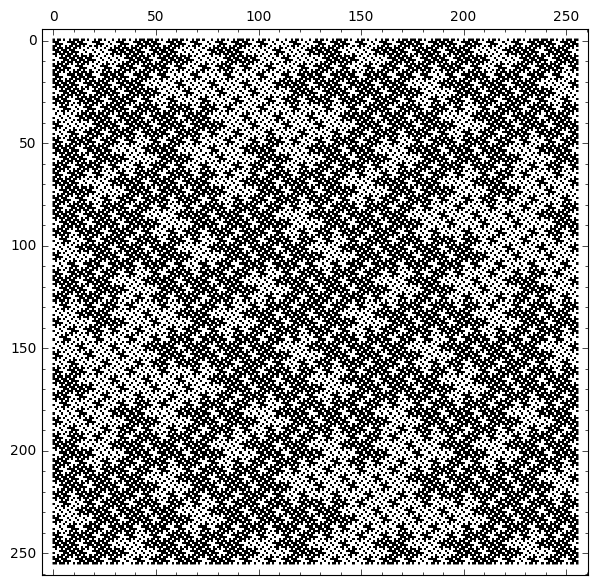
\includegraphics[width=.9\linewidth]{sigma_4_bent_cayley_graph_index_matrix.png}
  \captionof{figure}{$[\sigma_4]$:\\2 extended Cayley classes}
  \label{fig:sigma_4_bent_cayley_graph_index_matrix}
\end{minipage}%
\begin{minipage}{.48\textwidth}
  \centering
  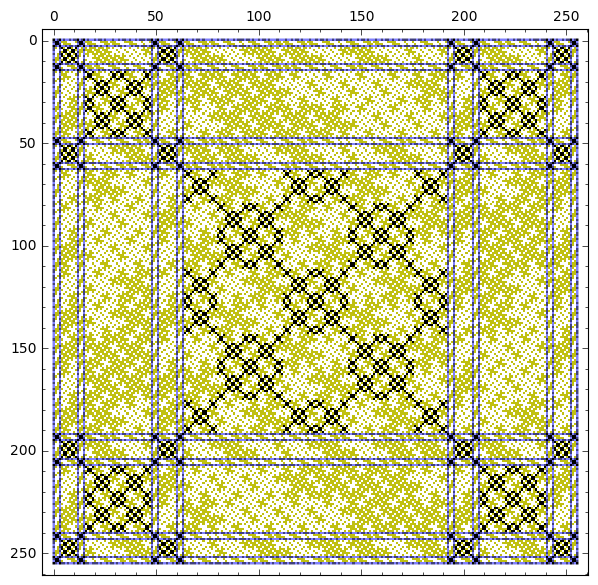
\includegraphics[width=.9\linewidth]{tau_4_bent_cayley_graph_index_matrix.png}
  \captionof{figure}{$[\tau_4]$:\\5 extended Cayley classes}
  \label{fig:tau_4_bent_cayley_graph_index_matrix}
\end{minipage}
\end{figure}
%\end{frame}
%\end{colortheme}
~
\newpage
~
\newpage
~
\newpage
%\paragraph*{Example CAST-128 S-Box ET class $[cast128_{1,0}]$.}
\subsection{CAST-128 S-boxes}
%
The CAST-128 encryption algorithm is used in PGP and elsewhere \cite{Ada97}.
The algorithm uses 8 S-boxes, each of which consists of 32 Boolean bent functions in 8 dimensions,
with degree 4, making 256 bent functions in total.
The full CAST-128 algorithm, including the contents of the S-boxes,
is published as IETF Request For Comments 2144 \cite{RFC2144}.

The bent function $cast128_{1,0}$ is the first bent function of S-box number 1 of CAST-128.
Its definition by algebraic normal form is
\footnotesize{}
\begin{align*}
cast128_{1,0} :=
\begin{array}{l}
x_{0} x_{1} x_{2} x_{3} + x_{0} x_{1} x_{2} x_{4} + x_{0} x_{1} x_{2} x_{5} + x_{0} x_{1} x_{2} + x_{0} x_{1} x_{3} x_{5} + x_{0} x_{1} x_{3} x_{6}\, +
\\
x_{0} x_{1} x_{3} + x_{0} x_{1} x_{5} x_{6} + x_{0} x_{1} x_{6} + x_{0} x_{1} x_{7} + x_{0} x_{2} x_{3} x_{4} + x_{0} x_{2} x_{3}\, +
\\
x_{0} x_{2} x_{4} x_{5} + x_{0} x_{2} x_{5} x_{7} + x_{0} x_{2} x_{6} + x_{0} x_{2} x_{7} + x_{0} x_{2} + x_{0} x_{3} x_{4} x_{5}\, +
\\
x_{0} x_{3} x_{4} x_{6} + x_{0} x_{3} x_{5} x_{6} + x_{0} x_{3} + x_{0} x_{4} x_{5} x_{6} + x_{0} x_{4} x_{5} x_{7} + x_{0} x_{4} x_{5}\, +
\\
x_{0} x_{4} x_{6} + x_{0} x_{4} + x_{0} x_{5} x_{6} + x_{0} x_{5} x_{7} + x_{0} x_{6} + x_{0} x_{7} + x_{0} + x_{1} x_{2} x_{4} x_{6}\, +
\\
x_{1} x_{2} x_{4} x_{7} + x_{1} x_{2} x_{5} x_{6} + x_{1} x_{2} x_{7} + x_{1} x_{3} x_{4} x_{6} + x_{1} x_{3} x_{4} x_{7} + x_{1} x_{3} x_{5}\, +
\\
x_{1} x_{3} x_{7} + x_{1} x_{4} x_{5} x_{7} + x_{1} x_{4} x_{6} + x_{1} x_{5} x_{6} + x_{1} + x_{2} x_{3} x_{4} x_{6} + x_{2} x_{3} x_{4}\, +
\\
x_{2} x_{3} x_{5} x_{6} + x_{2} x_{3} x_{5} + x_{2} x_{3} x_{7} + x_{2} x_{4} + x_{2} x_{5} x_{6} + x_{2} x_{5} + x_{2} + x_{3} x_{4} x_{5} x_{6}\, +
\\
x_{3} x_{5} x_{6} + x_{3} x_{5} x_{7} + x_{3} x_{6} + x_{3} + x_{4} + x_{6} x_{7}.
\end{array}
\end{align*}
\normalsize{}

This bent function $cast128_{1,0}$ is prolific:
the ET class $[cast128_{1,0}]$ contains the maximum possible number of Cayley classes,
that is $65\,536$.
The duals of the bent functions $[cast128_{1,0}]$ give another $65\,536$ extended Cayley classes.
In other words, no bent function in $[cast128_{1,0}]$ is EA equivalent to its dual.
The two weight classes of $[cast128_{1,0}]$ are
shown in Figure~\ref{fig:cast128_1_0_weight_class_matrix}.

\begin{figure}[!hb]
\centering
\begin{minipage}{.48\textwidth}
  \centering
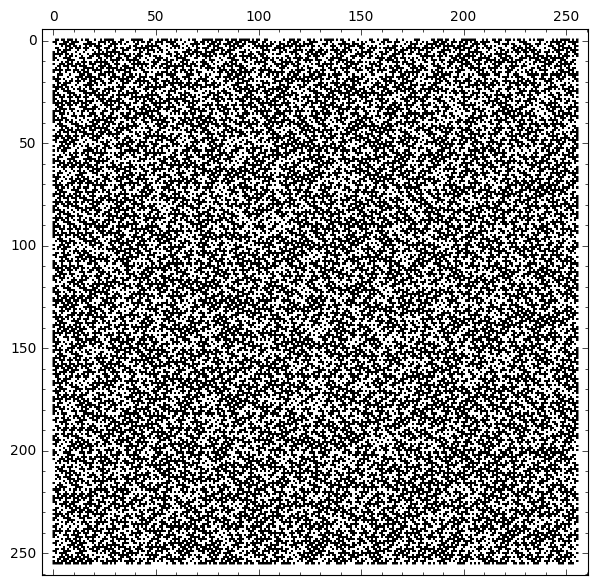
\includegraphics[width=.9\linewidth]{cast128_1_0_weight_class_matrix.png}
  \captionof{figure}{$[cast128_{1,0}]$:\\Weight classes ~~~~~~ ~~~~~~~~\\~\\Colormap: gist\_stern.}
  \label{fig:cast128_1_0_weight_class_matrix}
\end{minipage}
\begin{minipage}{.48\textwidth}
  \centering
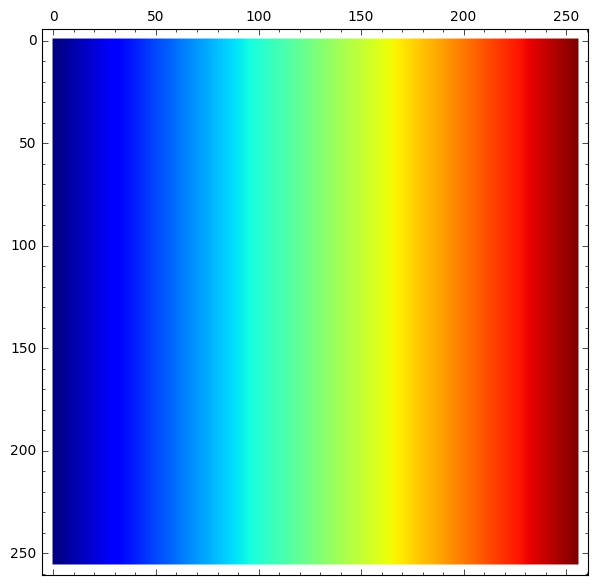
\includegraphics[width=.9\linewidth]{cast128_1_0_bent_cayley_graph_index_matrix.png}
  \captionof{figure}{$[cast128_{1,0}]$:\\$65\,536$ extended Cayley classes.\\Total including duals is $131\,072$.
\\Colormap: jet.}
  \label{fig:cast128_1_0_bent_cayley_graph_index_matrix}
\end{minipage}%
\end{figure}
%\frametitle{CAST-128 ET classes $[cast128_{2,1}]$ and $[cast128_{2,16}]$}

\begin{figure}[!ht]
\centering
\begin{minipage}{.48\textwidth}
  \centering
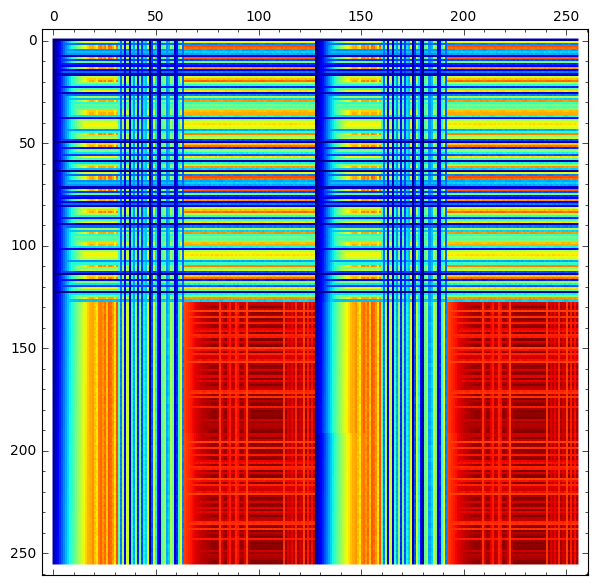
\includegraphics[width=.9\linewidth]{cast128_2_1_bent_cayley_graph_index_matrix.png}
  \captionof{figure}{$[cast128_{2,1}]$:\\$8\,256$ extended Cayley classes.\\Total including duals is $8\,256$.
\\Colormap: jet.}
  \label{fig:cast128_2_1_bent_cayley_graph_index_matrix}
\end{minipage}%
\begin{minipage}{.48\textwidth}
  \centering
\includegraphics[width=.9\linewidth]{cast128_2_16_bent_cayley_graph_index_matrix.png}
  \captionof{figure}{$[cast128_{2,16}]$:\\$32\,768$ extended Cayley classes.\\Total including duals is $65\,536$.
\\Colormap: jet.}
  \label{fig:cast128_2_16_bent_cayley_graph_index_matrix}
\end{minipage}%
\end{figure}
%\frametitle{CAST-128 ET classes $[cast128_{4,27}]$ and $[cast128_{5,16}]$}
\begin{figure}[!hb]
\centering
\begin{minipage}{.48\textwidth}
  \centering
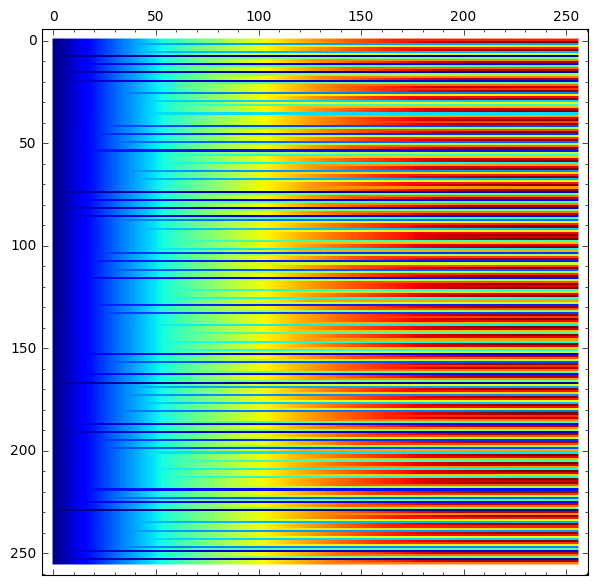
\includegraphics[width=.9\linewidth]{cast128_4_27_bent_cayley_graph_index_matrix.png}
  \captionof{figure}{$[cast128_{4,27}]$:\\$65\,536$ extended Cayley classes.\\Total including duals is $65\,536$.
\\Colormap: jet.}
  \label{fig:cast128_4_27_bent_cayley_graph_index_matrix}
\end{minipage}%
\begin{minipage}{.48\textwidth}
  \centering
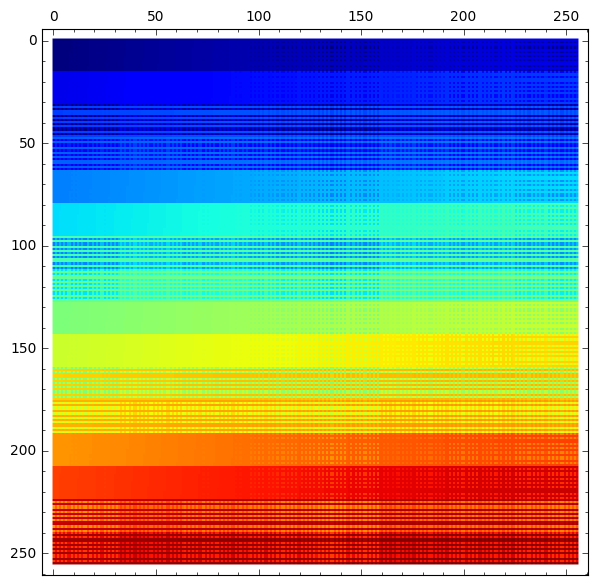
\includegraphics[width=.9\linewidth]{cast128_5_16_bent_cayley_graph_index_matrix.png}
  \captionof{figure}{$[cast128_{5,16}]$:\\$33\,280$ extended Cayley classes.\\Total including duals is $66\,560$.
\\Colormap: jet.}
  \label{fig:cast128_5_16_bent_cayley_graph_index_matrix}
\end{minipage}%
\end{figure}
%\frametitle{CAST-128 ET classes $[cast128_{5,27}]$ and $[cast128_{6,17}]$}
\begin{figure}[!ht]
\centering
\begin{minipage}{.48\textwidth}
  \centering
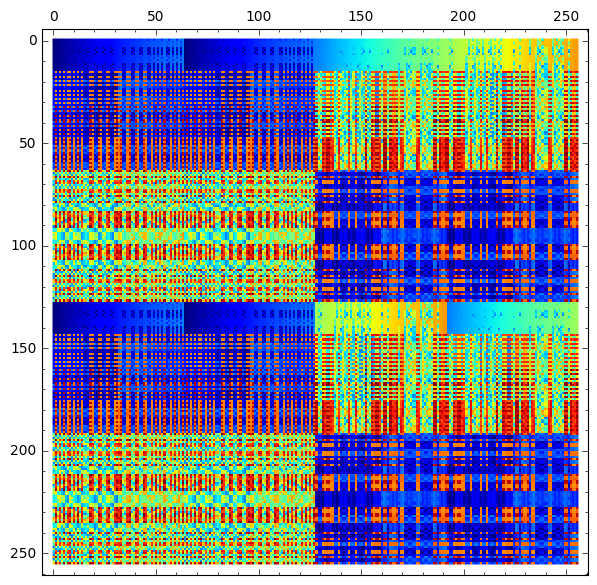
\includegraphics[width=.9\linewidth]{cast128_5_27_bent_cayley_graph_index_matrix.png}
  \captionof{figure}{$[cast128_{5,27}]$:\\$6\,144$ extended Cayley classes.\\Total including duals is $6\,144$.
\\Colormap: jet.}
  \label{fig:cast128_5_27_bent_cayley_graph_index_matrix}
\end{minipage}%
\begin{minipage}{.48\textwidth}
  \centering
\includegraphics[width=.9\linewidth]{cast128_6_17_bent_cayley_graph_index_matrix.png}
  \captionof{figure}{$[cast128_{6,17}]$:\\$65\,536$ extended Cayley classes.\\Total including duals is $65\,536$.
\\Colormap: jet.}
  \label{fig:cast128_6_17_bent_cayley_graph_index_matrix}
\end{minipage}%
\end{figure}
%\frametitle{CAST-128 ET classes $[cast128_{7,15}]$ and $[cast128_{7,21}]$}
\begin{figure}[!ht]
\centering
\begin{minipage}{.48\textwidth}
  \centering
\includegraphics[width=.9\linewidth]{cast128_7_15_bent_cayley_graph_index_matrix.png}
  \captionof{figure}{$[cast128_{7,15}]$:\\$32\,768$ extended Cayley classes.\\Total including duals is $65\,536$.
\\Colormap: jet.}
  \label{fig:cast128_7_15_bent_cayley_graph_index_matrix}
\end{minipage}%
\begin{minipage}{.48\textwidth}
  \centering
\includegraphics[width=.9\linewidth]{cast128_7_21_bent_cayley_graph_index_matrix.png}
  \captionof{figure}{$[cast128_{7,21}]$:\\$32\,768$ extended Cayley classes.\\Total including duals is $65\,536$.
\\Colormap: jet.}
  \label{fig:cast128_7_21_bent_cayley_graph_index_matrix}
\end{minipage}%
\end{figure}

Of the 256 bent functions that make up the 8 S-boxes of CAST-128, 248 are like $cast128_{1,0}$,
they are prolific and are not EA equivalent to their duals.
The remaining 8 bent functions are exceptional.
Both $cast128_{4,27}$ and $cast128_{6,17}$ are prolific, but both are EA equivalent to their duals.
\newpage

The other 6 bent functions are not prolific and the number of Cayley classes for each is given in the captions to
Figures \ref{fig:cast128_2_1_bent_cayley_graph_index_matrix} to \ref{fig:cast128_7_21_bent_cayley_graph_index_matrix}.
\subsection{Partial spread bent functions.}

According to Langevin and Hou \cite{LanH11counting}
there are $70\,576\,747\,237\,594\,114\,392\,064 \approx 2^{75.9}$ \Emph{partial spread} bent functions in
dimension 8,
contained in $14\,758$ EA classes.
The EA class representatives are listed at Langevin's web page \cite{Lan10psf}.
On this web page,
the file \texttt{psf-8.txt} contains details of $9316$ representatives that are
$\mathcal{PS}^{(-)}$ bent functions, all of degree 4; and
the file \texttt{psf-9.txt} contains details of $5442$ representatives that are
$\mathcal{PS}^{(+)}$ bent functions, of which $5440$ are of degree 4.

Preliminary calculations using SageMath on the NCI Raijin supercomputer indicate that
\begin{enumerate}
 \item
The $5442$ EA classes of $\mathcal{PS}^{(+)}$ bent functions of dimension 8
contain $296\,594\,720$ extended Cayley classes, assuming that each extended Cayley class appears in only one of the EA classes.
 \item
If the duals of the $5442$ representatives, and their corresponding EA classes are included,
the total number of extended Cayley classes is $541\,700\,450$, under the same assumption.
 \item
Of the $5442$ representatives,
$3434$ are prolific and not EA equivalent to their dual,
$582$ are prolific and are EA equivalent to their dual,
and the EA classes of the remaining $1426$ each contain less than $65\,536$ extended Cayley classes.
\end{enumerate}
The classifications of these $5442$ EA classes take up 2.1TB of space on the NCI Raijin supercomputer,
and it is intended that these classifications will be incorporated into a public database, if support can be found to maintain it
\cite{Leo18Database}.
%\slidecite{Langevin and Hou 2011}
% \end{frame}
% \end{colortheme}
% \begin{colortheme}{jubata}
% \begin{frame}
%\paragraph*{Example partial spread ET class $[psf_{9,5439}]$.}

%There are obviously too many bent functions of these two types to list here, but there is room for one example.

One example classification from $\mathcal{PS}^{(+)}$ in dimension 8 is that of $psf_{9,5439}$.
The bent function $psf_{9,5439}$ is listed as function number $5439$ in \texttt{psf-9.txt},
and is a $\mathcal{PS}^{(+)}$ bent function of degree 4.
Its ET class $[psf_{9,5439}]$ contains 16 extended Cayley classes,
of which 6 form three duality pairs similar to those seen in $[f_{8,9}]$ and $[f_{8,10}]$ above.

The 16 extended Cayley classes are distributed
as shown in Figures~\ref{fig:psf_9_5439_bent_cayley_graph_index_matrix} (classes) and~\ref{fig:psf_9_5439_dual_cayley_graph_index_matrix}
(classes of duals).

\begin{figure}[!ht] % [H]
\centering
\begin{minipage}{.48\textwidth}
  \centering
  \includegraphics[width=.9\linewidth]{psf_9_5439_bent_cayley_graph_index_matrix.png}
  \captionof{figure}{$[psf_{9,5439}]$:\\extended Cayley classes ~~ ~~~~ ~~~~\\~~~~~~~~~}
  \label{fig:psf_9_5439_bent_cayley_graph_index_matrix}
\end{minipage}
~~
\begin{minipage}{.48\textwidth}
  \centering
  \includegraphics[width=.9\linewidth]{psf_9_5439_dual_cayley_graph_index_matrix.png}
  \captionof{figure}{$[psf_{9,5439}]$:\\extended Cayley classes of dual bent\\functions}
  \label{fig:psf_9_5439_dual_cayley_graph_index_matrix}
\end{minipage}%
\end{figure}

% \end{frame}

%%%%%%%%%%%%%%%%%%%%%%%%%%%%%%%%%%%%%%%%%%%%%%%%%%%%%%%%%%%%%%%%%%%%%%

%\addtocontents{toc}{\vspace{0.5cm}}

\newpage

%\bibliographystyle{abbrv-par}

%\bibliography{bib}

\documentclass[12pt,a4paper]{article}
%
\usepackage{amsmath}
\usepackage{amssymb}
\usepackage{amsthm}
\usepackage{graphicx}
%
\usepackage[colorlinks=true,allcolors=blue]{hyperref}
\usepackage[figurename={Figure}]{caption}
\usepackage{float}
\usepackage{placeins}
%\usepackage{url}
%
\newcommand{\mb}[1]{\mathbb{#1}}
\newcommand{\mf}[1]{\mathbf{#1}}
\newcommand{\F}{\mb{F}}
\newcommand{\G}{\mb{G}}
\newcommand{\R}{\mb{R}}
\newcommand{\Z}{\mb{Z}}
\newcommand{\abs}[1]{\left| #1 \right|}
\newcommand{\norm}[1]{\left\| #1 \right\|}
\newcommand{\isomorphic}{\simeq}
\newcommand{\To}{\rightarrow}
%
%
%\newcommand{\slidecite}[1]{\tiny{(#1)}\normalsize{}}
%\newcommand{\smallcite}[1]{\small{(#1)}\normalsize{}}

\newcommand{\Emph}[1]{\emph{\textcolor{blue}{#1}}}

\newcommand{\Cay}[1]{\operatorname{Cay}\left(#1\right)}
\newcommand{\Clique}[1]{\omega\left(#1\right)}
\newcommand{\diag}[1]{\operatorname{diag}\left(#1\right)}
\newcommand{\dual}[1]{\widetilde{#1}}
\newcommand{\support}[1]{\operatorname{supp}\left(#1\right)}
\newcommand{\weight}[1]{\operatorname{wt}\left(#1\right)}
\newcommand{\weightclass}[1]{\operatorname{wc}\left(#1\right)}

\newtheorem*{lemma}{Lemma}
\newtheorem{Lemma}{Lemma}
\newtheorem*{proposition}{Proposition}
\newtheorem{Proposition}{Proposition}
\newtheorem*{theorem}{Theorem}
\newtheorem{Theorem}{Theorem}
\newtheorem*{conjecture}{Conjecture}
\newtheorem{Conjecture}{Conjecture}
\newtheorem*{corollary}{Corollary}
\newtheorem{Corollary}[Lemma]{Corollary}
\newtheorem*{remark}{Remark}
\newtheorem{Remark}{Remark}
\newtheorem*{definition}{Definition}
\newtheorem{Definition}{Definition}
\newtheorem{Question}{Question}
\newtheorem{Questions}[Question]{Questions}
%
\newenvironment{proofof}[1]{\noindent\emph{Proof of #1.}}{\qed}

\title{Classifying bent functions by their Cayley graphs}

\author{
Paul~Leopardi
%\thanks{Australian Government -- Bureau of Meteorology
\thanks{University of Melbourne; Australian Government -- Bureau of Meteorology
\protect\url{mailto:paul.leopardi@gmail.com}}
%\protect\texttt{mailto:paul.\-leopardi@anu.edu.au}}
}

\date{7 January 2018}

\begin{document}

\maketitle

\begin{abstract}
%
In 1999 Bernasconi and Codenotti noted that the Cayley graph of a bent function is strongly regular.
This paper describes the concept of extended Cayley equivalence of bent functions,
discusses some connections between bent functions, designs, and codes,
and explores the relationship between extended Cayley equivalence and extended affine equivalence.
SageMath scripts and CoCalc worksheets are used to compute and display some of these relationships,
for bent functions up to dimension 8.
%
\end{abstract}

\section{Introduction}
\label{sec-Introduction}
Binary bent functions are important combinatorial objects.
Besides the well-known application of bent functions and their generalizations to cryptography
\cite{Ada97} \cite[4.1-4.6]{Tok15bent},
bent functions have well-studied connections to Hadamard difference sets \cite{Dil74},
symmetric designs with the symmetric difference property \cite{DilS87block,Kan75symplectic},
projective two-weight codes \cite{DinD15class} and strongly regular graphs.

In two papers, Bernasconi and Codenotti \cite{BerC99}, and then Bernasconi, Codenotti and Vanderkam
\cite{BerCV01} explored some of the connections
between bent functions and strongly regular graphs.
While these papers established that the Cayley graph of a binary bent function (whose value at 0 is
0) is a strongly regular graph
with certain parameters, they leave open the question of which strongly regular graphs with these
parameters are so obtained.

In a recent paper \cite{Leo17Hurwitz},
the author found an example of two infinite series of bent functions whose
Cayley graphs have the same strongly regular parameters at each dimension,
but are not isomorphic if the dimension is 8 or more.

Kantor, in 1983 \cite{Kan83exponential}, showed that the numbers of non-isomorphic projective linear
two weight codes with certain parameters,
Hadamard difference sets, and symmetric designs with certain properties, grow at least exponentially
with dimension.
This result suggests that the number of strongly regular graphs obtained as Cayley graphs of bent
functions also increases at least exponentially with dimension.

The goal of the current paper is to further explore the connections between bent functions, their
Cayley graphs, and related combinatorial objects,
and in particular to examine the relationship between various equivalence classes of bent
functions, in particular, the relationship between the extended affine
equivalence classes and equivalence classes defined by isomorphism of Cayley graphs.
As well as a theoretical study of bent functions of all dimensions, an computational study is conducted
into bent functions of dimension at most 8,
using SageMath \cite{SageMath7517} and CoCalc \cite{CoCalc}.

The theoretical results of this paper serve a few purposes.
First, in order to classify bent functions by their Cayley graphs,
it helps to understand the relationship between Cayley equivalence and other concepts of equivalence
of bent functions, especially if this helps to cut down the search space needed for the
classification.
A similar consideration applies to the duals of bent functions.
Second, some of the empirical observations made in the classification of bent functions in small
dimensions can be explained by these theoretical results.
Third, these theoretical results can improve our understanding of the relationships between
bent functions, projective two-weight codes, strongly regular graphs, and
symmetric block designs with the symmetric difference property.
In what follows, known results are presented as propositions, with references;
and new results are presented as lemmas or theorems, with proofs.

% Two recent papers \cite{Leo14Constructions,Leo15Twin} describe and investigate two infinite sequences of bent functions and their Cayley graphs.
% The bent function $\sigma_m$ on $\F_2^{2 m}$ is described in the first paper \cite{Leo14Constructions}, on
% generalizations of Williamson's construction for Hada\-mard matrices.
% The bent function $\tau_m$ on $\F_2^{2 m}$ is described in the second paper \cite{Leo15Twin},
% which investigates some of the properties of the two sequences of bent functions.
% In this second paper it is shown that the bent functions $\sigma_m$ and $\tau_m$ both correspond to Hada\-mard difference sets with the same parameters
% \begin{align*}
% (v_m,k_m,\lambda_m,n_m) &= (4^m, 2^{2 m - 1} - 2^{m-1}, 2^{2 m - 2} - 2^{m-1}, 2^{2 m - 2}),
% \end{align*}
% and that their corresponding Cayley graphs are both strongly regular with the same parameters $(v_m,k_m,\lambda_m,\lambda_m)$.
%
% The main result of the current paper is the following.
% \begin{Theorem}\label{HR-non-imomorphic-theorem}
% The Cayley graphs of the bent functions $\sigma_m$ and $\tau_m$ are isomorphic only when $m=1, 2,$ or $3.$
% \end{Theorem}
%
The remainder of the paper is organized as follows.
% Section \ref{sec-Background} outlines some of the background of this investigation.
Section~\ref{sec-Preliminaries} covers the concepts, definitions and known results used later in the paper.
Section~\ref{sec-Bent-graphs} discusses the relationship between bent functions and strongly regular graphs.
Section~\ref{sec-Equivalence} introduces various concepts of equivalence of bent functions.
Section~\ref{sec-Bent-designs} discusses the relationship between bent functions and block designs.
%Section \ref{sec-Results} contains the main theoretical results of the paper.
Section~\ref{sec-Code} describes the SageMath and CoCalc code that has been used to obtain
the computational results of this paper.
Section~\ref{sec-Discussion} puts the results of this paper in the context of questions that are still open.
The appendices contain the proof of one of the properties of quadratic bent functions,
and list some of the properties of the equivalence classes of bent functions for dimension up to 8.

%
% % \begin{frame}
% \subsection{Overview}
% %\begin{center}
% \begin{itemize}
% \item
% Key concepts.
%
% ~
%
% \item
% Equivalence.
%
% ~
%
% \item
% Some results.
%
% ~
%
% \item
% Observations for small dimensions.
%
% ~
%
% \item
% Some questions.
%
% ~
%
% \item
% CoCalc worksheet.
% \end{itemize}

%\end{center}
% \end{frame}

% \section{Background}\label{sec-Background}
% A recent paper of the author \cite{Leo14Constructions} describes a generalization of
% Williamson's construction for Hada\-mard matrices \cite{Wil44}
% using the real monomial representation of the basis elements of the Clifford algebras $\R_{m,m}$.
% In that paper, the following three conjectures appear:
%
% \begin{Conjecture}\label{conjecture-1}
% %
% For all $m \geqslant 0$ there is a permutation $\pi$ of the set of $4^m$ canonical basis matrices,
% that sends an amicable pair of basis matrices with disjoint support to an anti-amicable pair, and
%vice-versa.
% %
% \end{Conjecture}
%
% \begin{Conjecture}\label{conjecture-2}
% %
% For all $m \geqslant 0,$
% for the Clifford algebra $\R_{m,m},$ the subset of transversal graphs that are
% not self-edge-colour complementary
% can be arranged into a set of pairs of graphs with each member of the pair
% being edge-colour complementary to the other member.
% %
% \end{Conjecture}
%
% \begin{Conjecture}\label{conjecture-3}
% %
% For all $m \geqslant 0,$
% for the Clifford algebra $\R_{m,m},$ if a graph $T$ exists amongst the transversal graphs,
% then so does at least one graph with edge colours complementary to those of $T$.
% %
% \end{Conjecture}
%
% The author's subsequent paper on bent functions \cite{Leo15Twin}
% refines Conjecture~\ref{conjecture-1} into the following question.
% \begin{Question}
% \label{Question-1}
% Consider the sequence of edge-coloured graphs $\varDelta_m$ for $m \geqslant 1$,
% each with red subgraph $\varDelta_m[-1],$ and blue subgraph $\varDelta_m[1].$
% For which $m \geqslant 1$ is there an automorphism of $\varDelta_m$
% that swaps the subgraphs $\varDelta_m[-1]$ and $\varDelta_m[1]$?
% \end{Question}
%
% (The term \emph{transversal graph} and the definitions of $\varDelta_m$, $\varDelta_m[-1],$ and
%$\varDelta_m[1]$
% are given in the relevant papers and are repeated in the next section.)
%
% The main result of this paper, Theorem \ref{HR-non-imomorphic-theorem} leads to the resolution of
%these conjectures and this question.

%\section{Key concepts}
\section{Preliminaries}
\label{sec-Preliminaries}

% \begin{frame}
This section presents some of the key concepts used in the remainder of the paper.
We first define bent functions, and then explore the relationships between bent functions
and Hamming weights.

% \begin{frame}
\subsection{Bent functions}

Here and in the remainder of the paper, $\F_2$ denotes the field of two elements,
also known as $GF(2)$. Models of $\F_2$ include integer arithmetic modulo 2
($\Z/2\Z$ also known as $\Z_2$) and Boolean algebra with ``exclusive or'' as addition and ``and''
as multiplication.

Bent Boolean functions can be defined in a number of equivalent ways.
The definition used here involves the Walsh Hadamard Transform.
\begin{Definition}
\label{def-Walsh-Hadamard-transform}
The Walsh Hadamard transform of
a Boolean function $f : \F_2^{2m} \To \F_2$ is
\begin{align*}
W_f(x)
&:=
\sum_{y \in \F_2^{2m}} (-1)^{f(y) + \langle x, y \rangle}
\end{align*}
\end{Definition}

\begin{Definition}
\label{def-Bent-function}
A Boolean function $f : \F_2^{2m} \To \F_2$ is \Emph{bent}
if and only if its Walsh Hada\-mard transform has constant absolute value $2^{m}$ \cite[p. 74]{Dil74}
\cite[p. 300]{Rot76}.
\end{Definition}

The remainder of this paper refers to bent Boolean functions simply as bent functions.

Remark: Bent functions can also be characterized as those Boolean functions whose Hamming distance
from any affine Boolean function is the maximum possible \cite[Ch. 14 Theorem 6]{MacS77} \cite[Theorem 3.3]{MeiS90}.

The characterization of bent functions given by Definition~\ref{def-Bent-function} immediately
implies the existence of dual functions:
\begin{Definition}
\label{def-dual-Bent-function}
For a bent function $f : \F_2^{2m} \To \F_2$, the function $\dual{f}$, defined by
\begin{align*}
(-1)^{\dual{f}(x)} &:= 2^{-m} W_f(x)
\end{align*}
is called the \Emph{dual} of $f$ \cite{CarDPS10self}.

Remark: The function $\dual{f}$ is also a bent function on $\F_2^{2m}$ \cite[p. 427]{MacS77} \cite[p. 301]{Rot76}.
\end{Definition}

\subsection{Weights and weight classes}
\begin{Definition}
\label{def-weight}
The \Emph{Hamming weight} of a Boolean function is the cardinality of its \Emph{support} \cite[p. 8]{MacS77}.
For $f$ on $\F_2^{2m}$
\begin{align*}
\support{f} &:= \{x \in \F_2^{2m} \mid f(x)=1 \}, \quad \weight{f} := \abs{ \support{f} }.
\end{align*}
\end{Definition}

The remainder of this paper refers to Hamming weights simply as weights.

Since a bent function of a given dimension can have only one of two weights,
the weights can be used to define equivalence classes of bent functions % and their Cayley graphs,
here called \emph{weight classes}.
\begin{Definition}
\label{def-weight-class}
A bent function $f$ on $\F_2^{2m}$ has weight \cite[Theorem 6.2.10]{Dil74}
\begin{align*}
\weight{f} &= 2^{2 m - 1} - 2^{m-1} \quad (\text{weight class number~} \weightclass{f}=0),
\text{~or}
\\
\weight{f} &= 2^{2 m - 1} + 2^{m-1} \quad (\text{weight class number~} \weightclass{f}=1).
\end{align*}
% If $f(0)=0$ then $\weightclass{\Cay{f}} := \weightclass{f}$.
\end{Definition}
% \end{frame}

\paragraph*{Weight classes and dual bent functions.}
%\subsection{Weight classes and dual bent functions.}

We now note a connection between weight classes and dual bent functions that
makes it a little easier to reason about dual bent functions.
The following lemma expresses the dual bent function in terms of weight classes.

\begin{Lemma}
\label{lm-notes-9b}
For a bent function $f : \F_2^{2m} \To \F_2$, and $x \in \F_2^{2m}$,
\begin{align*}
\dual{f}(x)
&=
\weightclass{y \mapsto f(y) + \langle x, y \rangle}
\end{align*}

\end{Lemma}

The proof of Lemma~\ref{lm-notes-9b} relies on the following lemma about weight classes.
\begin{Lemma}
\label{lm-notes-9a}
For a bent function $f : \F_2^{2m} \To \F_2$,
\begin{align*}
\weightclass{f}
&=
2^{-m} \weight{f} - 2^{m-1} + 2^{-1},
\intertext{so that}
\weight{f}
&=
2^{m} \weightclass{f} + 2^{2m-1} - 2^{m-1}.
\end{align*}

\end{Lemma}

\begin{proof}
If $\weight{f} = 2^{2 m - 1} - 2^{m-1}$ then
\begin{align*}
2^{-m} \weight{f} - 2^{m-1} + 2^{-1}
&=
2^{-m} (2^{2 m - 1} - 2^{m-1}) - 2^{m-1} + 2^{-1}
\\
&=
2^{m-1} - 2^{-1}  - 2^{m-1} + 2^{-1} = 0.
\end{align*}
If $\weight{f} = 2^{2 m - 1} + 2^{m-1}$ then
\begin{align*}
2^{-m} \weight{f} - 2^{m-1} + 2^{-1}
&=
2^{-m} (2^{2 m - 1} + 2^{m-1}) - 2^{m-1} + 2^{-1}
\\
&=
2^{m-1} + 2^{-1}  - 2^{m-1} + 2^{-1} = 1.
\end{align*}
\end{proof}

\begin{proofof}{Lemma~\ref{lm-notes-9b}}
Let $h(y) := y \mapsto f(y) + \langle x, y \rangle.$
Then
\begin{align*}
(-1)^{\dual{f}(x)}
&=
2^{-m} \sum_{y \in \F_2^{2m}} (-1)^{f(y) + \langle x, y \rangle}
\\
&=
2^{-m} \left( \sum_{f(y) + \langle x, y \rangle = 0} 1 - \sum_{f(y) + \langle x, y \rangle = 1} 1
\right)
\\
&=
2^{-m} \left( 2^{2m} - 2 \weight{h} \right)
=
2^m - 2^{1-m} \weight{h}
\\
&=
2^m - 2^{1-m} (2^{m} \weightclass{h} + 2^{2m-1} - 2^{m-1})
\\
&=
2^m - 2 \weightclass{h} - 2^m + 1
=
1 - 2 \weightclass{h} = (-1)^{\weightclass{h}},
\end{align*}
where we have used Lemma~\ref{lm-notes-9a}.
\end{proofof}

%
%~
%
%\slidecite{Dillon 1974; Rothaus 1976; Tokareva 2011}
% \end{frame}

% \begin{frame}
\section{Bent functions and strongly regular graphs}
\label{sec-Bent-graphs}
This section defines the Cayley graph of a Boolean function,
and explores the relationships between bent functions, projective two-weight codes, and strongly regular graphs.
\subsection{The Cayley graph of a Bent function}

The Cayley graph of a bent function $f$ with $f(0)=0$ is defined
in terms of the Cayley graph for a general Boolean function with $f$ with $f(0)=0$.
\paragraph*{The Cayley graph of a Boolean function.}
%\begin{center}
\begin{Definition}
\label{def-Cayley-graph}
For a Boolean function $f : \F_2^{2 m} \To \F_2$, with $f(0)=0$ we consider the simple undirected
\emph{Cayley graph} $\Cay{f}$  \cite[3.1]{BerC99}
where the vertex set $V(\Cay{f}) = \F_2^{2 m}$ and for $i,j \in \F_2^{2 m}$, the edge $(i,j)$ is in
the edge set $E(\Cay{f})$ if and only if $f(i+j)=1$.
\end{Definition}
Note especially that in contrast with the paper of Bernasconi and Codenotti \cite{BerC99},
this paper defines Cayley graphs only for Boolean functions $f$ with $f(0)=0$,
since the use of Definition~\ref{def-Cayley-graph} with a function $f$ for which $f(0)=1$ would
result in a graph with loops rather than a simple graph.

%\slidecite{Bernasconi and Codenotti 1999} % BerC99
% \end{frame}
% \begin{frame}
\paragraph*{Bent functions and strongly regular graphs.}
%\begin{center}
We repeat below in Proposition~\ref{pr-Cayley-bent-strongly-regular}
the result of Bernasconi and Codenotti \cite{BerC99}
that the Cayley graph of a bent function is strongly regular.
The following definition is used to fix the notation used in this paper.
\begin{Definition}
\label{def-strongly-regular-graph}
%
A simple graph $\Gamma$ of order $v$ is \Emph{strongly regular} \cite{Bos63,BroCN89,Sei79} with
parameters
$(v,k,\lambda,\mu)$ if
\begin{itemize}
 \item
each vertex has degree $k,$
 \item
each adjacent pair of vertices has $\lambda$ common neighbours, and
\item
each nonadjacent pair of vertices has $\mu$ common neighbours.
\end{itemize}
%
\end{Definition}
%~
%
%\slidecite{Brouwer, Cohen and Neumaier 1989} % BroCN89

%\end{center}
% \end{frame}

% \begin{frame}
The following proposition summarizes some of the well-known properties of the Cayley graphs of bent functions.
\begin{Proposition}
\label{pr-Cayley-bent-strongly-regular}
The Cayley graph $\Cay{f}$ of a bent function $f$ on $\F_2^{2m}$
with $f(0)=0$ is a strongly regular graph with $\lambda = \mu$ \cite[Lemma 12]{BerC99}.

In addition, any Boolean function $f$ on $\F_2^{2m}$ with $f(0)=0$,
whose Cayley graph $\Cay{f}$ is a strongly regular graph with $\lambda = \mu$ is a bent function
\cite[Theorem 3]{BerCV01} \cite[Theorem 3.1]{Sta07}.

For a bent function $f$ on $\F_2^{2m}$,
the parameters of $\Cay{f}$ as a strongly regular graph
are \cite[Theorem 6.2.10]{Dil74} \cite[Theorem 3.2]{HuaY04}
\begin{align*}
(v,k,\lambda,\mu) = &(4^m, 2^{2 m - 1} - 2^{m-1}, 2^{2 m - 2} - 2^{m-1}, 2^{2 m - 2} - 2^{m-1})
\\
  \text{or} \quad &(4^m, 2^{2 m - 1} + 2^{m-1}, 2^{2 m - 2} + 2^{m-1}, 2^{2 m - 2} + 2^{m-1}).
\end{align*}
\end{Proposition}

%~
%
%\slidecite{Menon 1962; Dillon 1974; Bernasconi and Codenotti 1999}
%\end{center}
% \end{frame}
% \begin{frame}
\subsection{Bent functions, linear codes and strongly regular graphs}
Another well known way to obtain a strongly regular graph from a bent function is via a projective two-weight
code.
This is done via the following definitions.
\paragraph*{Projective two-weight binary codes.}

\begin{Definition}
\label{def-two-weight-codes}
\cite{BouFFWW2006} \cite{Ton96uniformly}

A \Emph{two-weight binary code} with parameters $[n,k,d]$ is a $k$ dimensional subspace of $\F_2^n$
with
minimum Hamming distance $d$, such that the set of Hamming weights of the non-zero vectors has size
2.

Bouyukliev, Fack, Willems and Winne \cite[p. 60]{BouFFWW2006} define projective codes as follows.
``A \Emph{generator matrix} $G$ of a linear code $[n, k]$ code $C$ is any matrix
of rank $k$ (over $\F_2$) with rows from $C.$ \ldots
A linear $[n, k]$ code is called \Emph{projective} if no two columns of a generator matrix
$G$ are linearly dependent, i.e., if the columns of $G$ are pairwise different points in a
projective $(k-1)$-dimensional space.''

Remark: In the case of $\F_2$, no two columns are equal.

A \Emph{projective two-weight binary code} with parameters $[n, k, d]$ is thus a
two-weight binary with these parameters which is also projective as an $[n, k]$ linear code.
%
%~
%
%\slidecite{Bouyukliev, Fack, Willems and Winne 2006} % BouFFWW2006
%
\end{Definition}

\paragraph*{From bent function to strongly regular graph via a projective two-weight code.}
There is a standard method of obtaining a projective two-weight code from a bent function in such a way that
the code can be used to define a bent function.
This method uses the following definition.
\begin{Definition}
\label{def-bent-two-weight-code}
\cite[Corollary 10]{DinD15class}
%\smallcite{Ding 2015, Corollary 10}

For a bent function $f : \F_2^{2m} \To \F_2$,
define the linear code $C(f)$ by the generator matrix
\begin{align*}
M_C(f)_{x,y} &\in \F_2^{2^{2m} \times \weight{f}},
\\
M_C(f)_{x,y} &:= \langle x, \support{f}(y) \rangle,
\end{align*}
with $x$ in lexicographic order of $\F_2^{2m}$
and $\support{f}(y)$ in lexicographic order of $\support{f}$.

The $4^m$ words of the code $C(f)$ are the rows of the generator matrix $M_C(f)$.
\end{Definition}

The linear code $C(f)$ so obtained has the following properties.
%\slidecite{Ding 2015, Corollary 10}
%
% \end{frame}
% \begin{frame}
%\frametitle{From bent function to linear code (2)}
\begin{Proposition}
\cite[Corollary 10]{DinD15class}
%\smallcite{Ding 2015, Corollary 10}

For a bent function $f : \F_2^{2m} \To \F_2$, the linear code $C(f)$
is a projective two-weight binary code.
%
%~
%
The possible weights of non-zero code words are:
\begin{align*}
\begin{cases}
2^{2m-2}, 2^{2m-2} - 2^{m-1} & \text{if~} \weightclass{f}=0.
\\
2^{2m-2}, 2^{2m-2} + 2^{m-1} & \text{if~} \weightclass{f}=1.
\end{cases}
\end{align*}
%
\end{Proposition}
%
%\slidecite{Ding 2015, Corollary 10}
%
% \end{frame}
% \begin{frame}
\paragraph*{From linear code to strongly regular graph.}
This paper uses the following non-standard definition to obtain a strongly regular graph from a
projective two-weight code.
\begin{Definition}
\label{R-f-def}
Given $f : \F_2^{2m} \To \F_2$, and linear code $C(f)$ defined as per Definition~\ref{def-bent-two-weight-code},
define the graph $R(f)$ as follows.

Vertices of $R(f)$ are code words of $C(f)$.

For code words $v,w \in C(f)$, edge $(u,v) \in R(f)$ if and only if
\begin{align*}
\begin{cases}
\weight{u+v} = 2^{2m-2} - 2^{m-1} & (\text{if~}\weightclass{f}=0).
\\
\weight{u+v} = 2^{2m-2} + 2^{m-1} & (\text{if~}\weightclass{f}=1).
\end{cases}
\end{align*}

\end{Definition}
Since $C(f)$ is a projective two-weight binary code,
$R(f)$ is a strongly regular graph \cite[Theorem 2]{Del72weights}.
The standard definition uses the lower of the two weights in both cases above.

%\slidecite{Delsarte 1972, Theorem 2}
% \end{frame}

% \end{frame}


% \end{frame}
%\subsection{Bent functions, linear codes and strongly regular graphs}
% \begin{frame}
\paragraph*{The graph $R(f)$ is the Cayley graph of the extended dual.}
The strongly regular graph $R(f)$ of bent function $f$, as defined by the non-standard Definition
\ref{R-f-def} has the following remarkable property.

\begin{Theorem}
For bent $f : \F_2^{2m} \To \F_2$, with $f(0)=0$,
\begin{align*}
R(f) \equiv \Cay{\dual{f} + \weightclass{f}}.
\end{align*}

\end{Theorem}
% \end{frame}
\begin{proof}
We examine $W_f$, the Walsh Hadamard transform of $f$.
\begin{align*}
W_f(y)
&=
\sum_{x \in \F_2^{2 m}} (-1)^{\langle x, y \rangle} + f(x)
=
\sum_{f(x)=0} (-1)^{\langle x, y \rangle} + f(x)
- 2\sum_{f(x)=1} (-1)^{\langle x, y \rangle}
\\
&=
\sum_{x \in \F_2^{2 m}} (-1)^{\langle x, y \rangle}
- 2\sum_{f(x)=1} (-1)^{\langle x, y \rangle}.
\end{align*}
But
\begin{align*}
\sum_{x \in \F_2^{2 m}} (-1)^{\langle x, y \rangle}
&=
\begin{cases}
4^m &(y=0)
\\
0 & \text{otherwise},
\end{cases}
\end{align*}
as per the Sylvester Hadamard matrices.

So, for $y \neq 0$,
\begin{align*}
W_f(y)
&=
- 2\sum_{f(x)=1} (-1)^{\langle x, y \rangle},
\intertext{so}
\sum_{f(x)=1} (-1)^{\langle x, y \rangle}
&=
\weight{f} - 2 \sum_{\substack{f(x)=1 \\ \langle x, y \rangle =1}} 1
=
- W_f(y)/2.
\intertext{But}
\sum_{\substack{f(x)=1 \\ \langle x, y \rangle =1}} 1
&=
\weight{C(f)[y]},
\end{align*}
the weight of code $C(f)$ at the point $y$.
So
\begin{align*}
\weight{f} - 2 \weight{C(f)[y]}
&=
- W_f(y)/2,
\intertext{and therefore}
\weight{C(f)[y]}
&=
\weight{f}/2 + W_f(y)/4.
\end{align*}
We now examine the two possible weight class numbers of $f$.

If $\weightclass{f} = 0$ then $\weight{f} = 2^{2m-1}-2^{m-1}$.
For $y \neq 0$ there are two cases, depending on $\dual{f}(y)$:

If $\dual{f}(y) = 0$ then $W_f(y) = 2^m$, so
\begin{align*}
\weight{C(f)[y]}
&=
2^{2m-2}-2^{m-2} + 2^{m-2}
=
2^{2m-2}
=
4^{m-1}.
\end{align*}

If $\dual{f}(y) = 1$ then $W_f(y) = -2^m$, so
\begin{align*}
\weight{C(f)[y]}
&=
2^{2m-2}-2^{m-2} - 2^{m-2}
=
2^{2m-2} - 2^{m-1}
=
4^{m-1} - 2^{m-1}.
\end{align*}

Similarly, if $\weightclass{f} = 1$ then $\weight{f} = 2^{2m-1}+2^{m-1}$,
and so for $y \neq 0$
\begin{align*}
\weight{C(f)[y]}
&=
\begin{cases}
4^{m-1} + 2^{m-1} & (\dual{f}(y)=0)
\\
4^{m-1}           & (\dual{f}(y)=1).
\end{cases}
\end{align*}
Also, as a consequence of Lemma \ref{lm-notes-9b}, $\weightclass{f} = \dual{f}(0)$,
so if $g(y) := \dual{f}(y) + \weightclass{f}$ then $g(0)=0$ and therefore the Cayley graph of $g$
is well defined.
\end{proof}

\section{Equivalence of bent functions}
\label{sec-Equivalence}
The following concepts of equivalence of Boolean functions are used in this paper,
usually in the case where the Boolean functions are bent.

% \begin{frame}
\paragraph*{Extended affine equivalence.}

\begin{Definition}
For Boolean functions $f,g : \F_2^{2m} \To \F_2$,
$f$ is \Emph{extended affine equivalent} to $g$ \cite[Section 1.4]{Tok15bent} if and only if
\begin{align*}
g(x) &= f(A x + b) + \langle c, x \rangle + \delta
\end{align*}
for some $A \in GL(2m,2)$, $b, c \in \F_2^{2m}$, $\delta \in \F_2$.
\end{Definition}

The Boolean $f$ is extended affine equivalent to $g$
if and only if $f$ and $g$ are in the same orbit
of the action of the \Emph{extended general affine group} $EGA(2m, 2)$ on $\F_2^{\F_2^{2m}}$, defined as follows.

\begin{Definition}
\begin{align*}
&EGA(2m, 2) := \{ (A,b,c,\delta) \mid A \in GL(2m,2),\ b, c \in \F_2^{2m},\ \delta \in \F_2 \}
\intertext{with}
&(A,b,c,\delta)(A',b',c',\delta') := (A A', A b' + b, A'^T c + c', \langle c, b' \rangle + \delta + \delta'),
\end{align*}
with action
\begin{align*}
(A,b,c,\delta)f(x) &:= f(A x + b) + \langle c, x \rangle + \delta,
\\
\left( (A,b,c,\delta)(A',b',c',\delta') f \right)
& := (A',b',c',\delta') \circ (A,b,c,\delta) f
\\
& = (A',b',c',\delta') \left( (A,b,c,\delta) f \right).
\end{align*}
\cite[Section 2]{Mai91}
\end{Definition}

% \begin{frame}
\paragraph*{General linear equivalence.}
\begin{Definition}
For Boolean functions $f,g : \F_2^{2m} \To \F_2$,
$f$ is \Emph{general linear equivalent} to $g$ if and only if
\begin{align*}
g(x) &= f(A x)
\end{align*}
for some $A \in GL(2m,2)$.
\end{Definition}

Thus $f$ is general linear equivalent to $g$
if and only if $f$ and $g$ are in the same orbit
of the action of the general linear group $GL(2m, 2)$ on $\F_2^{\F_2^{2m}}$, defined as follows.

\begin{Definition}
\begin{align*}
A f(x) &:= f(A x),
\\
(A A') f & := A' \circ A f = A' (A f).
\end{align*}
\end{Definition}
Some references for the study of the general linear equivalence of Boolean functions
include Harrison \cite{Har64}, Comerford \cite{Com80}, and Maiorana \cite[Section 2]{Mai91}.
% \begin{frame}
\paragraph*{Extended translation equivalence.}

\begin{Definition}
For Boolean functions $f,g : \F_2^{2m} \To \F_2$,
$f$ is \Emph{extended translation equivalent} to $g$ if and only if
\begin{align*}
g(x) &= f(x + b) + \langle c, x \rangle + \delta
\end{align*}
for $b, c \in \F_2^{2m}$, $\delta \in \F_2$.
\end{Definition}
% \end{frame}

Thus $f$ is extended translation equivalent to $g$
if and only if $f$ and $g$ are in the same orbit
of the action of the \Emph{extended translation group} $ET(2m, 2)$ on $\F_2^{\F_2^{2m}}$, defined as follows.

\begin{Definition}
\begin{align*}
&ET(2m, 2) := \{ (b,c,\delta) \mid \ b, c \in \F_2^{2m},\ \delta \in \F_2 \}
\intertext{with}
&(b,c,\delta)(b',c',\delta') := (b' + b, c + c', \langle c, b' \rangle + \delta + \delta'),
\end{align*}
with action
\begin{align*}
(b,c,\delta)f(x) &:= f(x + b) + \langle c, x \rangle + \delta,
\\
\left( (b,c,\delta)(b',c',\delta') \right) f
& := (b',c',\delta') \circ (b,c,\delta) f
\\
& = (b',c',\delta') \left( (b,c,\delta) f \right).
\end{align*}
\end{Definition}

%\slidecite{Tokareva 2014}
% \end{frame}
% \begin{frame}
\paragraph*{Cayley equivalence.}
\begin{Definition}
%
For Boolean functions $f, g : \F_2^{2m} \To \F_2$, with $f(0)=g(0)=0$,
we call $f$ and $g$ \Emph{Cayley equivalent},
and write $f \equiv g$,
if and only if the graphs $\Cay{f}$ and $\Cay{g}$ are isomorphic.

Equivalently, $f \equiv g$ if and only if
there exists a bijection $\pi : \F_2^{2m} \To \F_2^{2m}$ such that
\begin{align*}
g(x+y) &= f \big(\pi(x)+\pi(y)\big) \quad \text{for all~} x,y \in \F_2^{2m}.
\end{align*}
\end{Definition}
% \end{frame}
Remark: Note that the bijection $\pi$ is not necessarily linear on $\F_2^{2m}$.
Examples of bent functions $f$ and $g$ where $f \equiv g$ but the bijection is not linear
are given in Section~\ref{sec-Empirical}.
% \begin{frame}
\paragraph*{Extended Cayley equivalence.}
%
While Bernasconi and Codenotti \cite{BerC99} define Cayley graphs for Boolean functions with
$f(0)=1$ and allow Cayley graphs to have loops, this paper defines Cayley
graphs only for Boolean functions where $f(0)=0$.
This has the disadvantage that Cayley equivalence is an equivalence relation on half
of the Boolean functions rather than all of them.
To extend this equivalence relation to all Boolean functions,
we just declare the functions $f$ and $f+1$ to be ``extended'' Cayley equivalent,
resulting in the following definition.
\begin{Definition}
For Boolean functions $f, g : \F_2^{2m} \To \F_2$,
if there exist $\delta, \epsilon \in \{0,1\}$ such that $f + \delta \equiv g + \epsilon$,
we call $f$ and $g$ \Emph{extended Cayley (EC) equivalent} and write $f \cong g$.
\end{Definition}
Extended Cayley equivalence is thus an equivalence relation on the set of all Boolean functions on
$\F_2^{2m}$.
It is easy to verify that $f \cong g$ if and only if $f+f(0) \equiv g+g(0)$.

% \end{frame}

% \begin{frame}
\subsection{Relationships between different concepts of equivalence}
%\section{Theoretical results}
%\label{sec-Results}
% \begin{frame}

% This section contains a number of theoretical results that serve a few purposes.
% Firstly,
As stated in the Introduction, in order to classify bent functions by their Cayley graphs,
it helps to understand the relationship between Cayley equivalence and other concepts of equivalence
of Boolean functions, especially if this helps to cut down the search space needed for the classification.
This section lists a few of these useful relationships.

% A similar consideration applies to the duals of bent functions.
% Secondly, some empirical observations made in the classification of bent functions in small
% dimensions can be explained by theoretical results.
% Thirdly, theoretical results can improve our understanding of the relationships between
% some of the concepts introduced in the previous section, notably dual bent functions, SDP designs,
% projective two-weight codes, and strongly regular graphs.

\paragraph*{General linear equivalence implies Cayley equivalence.}

Firstly, general linear equivalence of Boolean functions implies Cayley equivalence.
Specifically, the following result applies.
\begin{Theorem}
\label{th-Linear-Cayley}
If $f$ is a Boolean function with $f(0)=0$ and $g(x) := f(A x)$ where $A \in GL(2m,2)$,
then $f \equiv g$.
\end{Theorem}
\begin{proof}
\begin{align*}
g(x+y) &= f\big(A(x+y)\big) = f(A x + A y)\quad \text{for all~} x,y \in \F_2^{2m}.
\end{align*}
\end{proof}
Thus, for bent functions, the following result holds.
\begin{Corollary}
\label{corr-bent-Linear-Cayley}
If $f$ is bent with $f(0)=0$ and $g(x) := f(A x)$ where $A \in GL(2m,2)$,
then $g$ is bent with $g(0)=0$ and $f \equiv g$.
\end{Corollary}
Thus if $f$ is bent with $f(0)=0$, and $g$ is bent with $g(0)=0$, and $f \not\equiv g$,
then $f$ is not general linear equivalent to $g$.
This result immediately leads to another corollary.
Here, and later in this paper, we make use of the following terminology.
\begin{Definition}
A Boolean function $f \mid \F_2^{n} \To \F_2$ is said to be \Emph{prolific} if
there is no pair $b, c \in \F_2^{n}$ with $g(x) = f(x+b) + \langle c, x \rangle + f(b)$ such that $f \cong g$.
Thus the number of extended Cayley classes in the extended translation class of a prolific Boolean function
is $4^n$.
\end{Definition}

\begin{Corollary}
 \label{corr-no-Cayley-no-Linear}
If $f \mid \F^{2m} \To \F_2$ is bent with $f(0)=0$, and $f$ is prolific, then there is no triple
$A \in GL(2m,2)$, $b, c \in \F_2^{2m}$ with $f(Ax) = f(x+b) + \langle c, x \rangle + f(b)$.
\end{Corollary}

% \end{frame}

% \begin{frame}
\paragraph*{Extended affine, translation, and Cayley equivalence.}

Secondly, if $f$ is a Boolean function,
and $h$ is a Boolean function $h$ that is extended affine equivalent to $f$,
then a Boolean function $g$ exists that is general linear equivalent to $h$
and extended translation equivalent to $f$:
\begin{Theorem}
\label{th-Affine-Translate-Linear}
For $A \in GL(2m,2)$, $b, c \in \F_2^{2m}$, $\delta \in \F_2$,
$f : \F_2^{2m} \To \F_2$,
the function
\begin{align*}
h(x) &:= f(A x + b) + \langle c, x \rangle + \delta
\intertext{can be expressed as $h(x) = g(A x)$ where}
g(x) &:= f(x+b) + \langle (A^{-1})^T c, x \rangle + \delta.
\end{align*}
\end{Theorem}
% \end{frame}
\begin{proof}
Let $y:= A x$. Then
\begin{align*}
g(A x) = g(y)
&= f(y+b) + \langle (A^{-1})^T c, y \rangle + \delta
\\
&= f(y+b) + \langle c, A^{-1} y \rangle + \delta
\\
&= f(A x + b) + \langle c, x \rangle + \delta = h(x).
\end{align*}
\end{proof}

\begin{Corollary}
\label{corr-Affine-Translate-Cayley}
If $f$ is a bent Boolean function,
and a bent function $h$ is extended affine equivalent to $f$,
then a bent function $g$ can be found that is extended Cayley equivalent to $h$
and extended translation equivalent to $f$.
\end{Corollary}
% \end{frame}
\begin{proof}
Let $f$, $g$, and $h$ be as per Theorem \ref{th-Affine-Translate-Linear}.
If $f$ is bent, then so are $g$ and $h$.
Since, by Theorem \ref{th-Affine-Translate-Linear}, $g$ is general linear equivalent to $h$,
by Theorem \ref{th-Linear-Cayley}, $g$ is extended Cayley equivalent to $h$.
\end{proof}

As a consequence, to determine which strongly regular graphs occur, corresponding to each
extended Cayley equivalence classes within the extended affine
equivalence class of a bent function $f : \F_2^{2m} \To \F_2$ with $f(0)=0$,
we need only examine the extended translation equivalent functions of the form
\begin{align*}
f(x+b) + \langle c, x \rangle + f(b),
\end{align*}
for each $b, c \in \F_2^{2m}$.
This cuts down the required search space considerably.

% \end{frame}

\paragraph*{Quadratic bent functions have only two extended Cayley classes.}
Finally, in the case of quadratic bent functions, there is a complete classification in terms of
weight classes.
\begin{Theorem}
\label{th-Quadratic-Classes}
For each $m>0$, the extended affine equivalence class of quadratic bent functions
$q : \F_2^{2m} \To \F_2$ contains exactly two extended Cayley equivalence classes,
corresponding to the two possible weight classes of
$x \mapsto q(x+b) + \langle c, x \rangle + q(b)$.
\end{Theorem}

The proof of this theorem is given in Appendix~\ref{app-proof-of}.

\subsection{Relationships between duality of bent functions and different concepts of equivalence}

The following propositions are based on well known results,
but are useful in understanding the relationship
between the duality of bent functions and various concepts of equivalence.
% \begin{frame}
%\subsection{Dual functions}

Firstly, general linear equivalence of bent functions $f$ and $g$
implies general linear equivalence of their duals, $\dual{f}$ and $\dual{g}$,
which implies Cayley equivalence of $\dual{f}$ and $\dual{g}$.
\begin{Proposition}
\label{prop-dual-linear-equivalence}
\cite[Remark 6.2.7]{Dil74}

For a bent function $f : \F_2^{2m} \To \F_2$, and $A \in GL(2 m, 2)$, if
\begin{align*}
g(x) &:= f(A x)
\intertext{then}
\dual{g}(x) &= \dual{f}\big((A^T)^{-1} x \big),
\end{align*}
and therefore by Theorem \ref{th-Linear-Cayley}, $\dual{g} \equiv \dual{f}$.

If, in addition, $f=\dual{f}$ then $\dual{g} \equiv g$.
\end{Proposition}

Remark: Functions of the form
\begin{align*}
f(x) := \sum_{k=0}^{m-1} x_{2k} x_{2k+1}
\end{align*}
are self dual bent functions, $f=\dual{f}$ \cite[Remark 6.3.2]{Dil74}.
There are many other self dual bent functions \cite{CarDPS10self,FeuSSW2013}.

Secondly, the following proposition displays a relationship between the extended translation
class of a bent function $f$, and that of its dual $\dual{f}$.
\begin{Proposition}
\label{prop-dual-affine-equivalence}
\cite[Remark 6.2.7]{Dil74} \cite[Proposition 8.7]{Car10boolean}.
%\smallcite{Carlet 2007, Proposition 4}
%
%~

For a bent function $f$ on $\F_2^{2m}$, and $b,c \in \F_2^{2m}$,
if
\begin{align*}
g(x) &:= f(x+b) + \langle c, x \rangle
\intertext{then}
\dual{g}(x) &= \dual{f}(x+c) + \langle b, x \rangle + \langle b, c \rangle.
\end{align*}
\end{Proposition}

This result has an implication for the relationship between the set of bent functions within
an extended translation (ET) equivalence class, and the set of their duals.
Recall that a bent function is not necessarily extended affine (EA) equivalent to its dual
\cite{LanLM08Kasami}.
The following ``all or nothing'' property holds within an extended translation equivalence class of bent functions.
\begin{Corollary}
\label{cor-dual-ET-EC}
For bent functions $f, g$ on $\F_2^{2m}$,
if $f$ is EA equivalent to $\dual{f}$ and $g$ is ET equivalent to $f$,
then $\dual{g}$ is EA equivalent to $g$.
Thus, by Corollary~\ref{corr-Affine-Translate-Cayley},
the set of isomorphism classes of Cayley graphs of the \Emph{duals} of the bent functions in
the ET class of $f$ equals the set of isomorphism classes of Cayley graphs of
the bent functions themselves.

Conversely, for a bent function $f$ on $\F_2^{2m}$,
if there is any bent function $g$ that is ET equivalent to $f$,
such that $\dual{g}$ is not EA equivalent to $g$, then no bent function in the ET class is EA
equivalent to its dual, including $f$ itself.
\end{Corollary}

% \begin{frame}

% \begin{frame}
\section{Bent functions and block designs}
\label{sec-Bent-designs}
% \begin{frame}
%\subsection{Weight classes, dual functions, and SDP designs}

This section examines the relationships between bent functions and symmetric block designs.

% \end{frame}

% \end{frame}
% \begin{frame}
%\subsection{Dual functions}

%~
%
%\slidecite{Carlet, Danielson, Parker and Sol\'e 2008; Feulner, Sok, Sol\'e and Wassermann 2011} %
%FeuSSW2013
% \end{frame}
\subsection{The two block designs of a bent function}

The first block design of a bent function $f$ on $\F_2^{2m}$ is obtained by interpreting
the adjacency matrix of $\Cay{f}$ as the incidence matrix of a block design.
In this case we do not need $f(0)=0$ \cite[p. 160]{DilS87block}.

The second block design of a bent function $f$ involves the
\Emph{symmetric difference property}, which was first investigated by Kantor
\cite[Section 5]{Kan75symplectic}.
\begin{Definition}
\label{def-Symmetric-difference-property}
\cite[p. 49]{Kan75symplectic}.

A symmetric block design $\mathcal{D}$ has the symmetric difference property (SDP)
if, for any three blocks, $B, C, D$ of $\mathcal{D},$ the symmetric difference
$B \bigtriangleup C \bigtriangleup D$ is either a block or the complement of a block.
\end{Definition}

This second block design is defined as follows.
\begin{Definition}
\label{def-SDP-design}
For a bent function  $f$ on $\F_2^{2m}$, define the matrix $M_D(f) \in \F_2^{2^{2m} \times 2^{2m}}$ where
\begin{align}
M_D(f)_{c,x} &:= f(x) + \langle c, x \rangle + \dual{f}(c),
\label{D-f-def}
\end{align}
and use it as the incidence matrix of a symmetric block design, which
we call it the \emph{SDP design} of $f$.
\end{Definition}

Kantor describes the special case where $f$ is quadratic
\cite[Section 5]{Kan75symplectic},
and Dillon and Schatz \cite{DilS87block} describe the general case.

The following properties of SDP designs of bent functions are well known.
\begin{Proposition}
\label{prop-SDP-design}
\cite[p. 160]{DilS87block} \cite[Theorem 3.29]{Neu06bent}

For any bent function $f$ on $\F_2^{2m}$, the SDP design of $f$ has the symmetric difference property.
\end{Proposition}

\begin{Proposition}
\label{prop-SDP-design-affine-equivalence}
\cite[p. 161]{DilS87block} \cite{Kan83exponential}

For bent functions $f, g$ on $\F_2^{2m}$,
the two SDP designs $D(f)$ and $D(g)$ are isomorphic as symmetric block designs
if and only if $f$ and $g$ are affine equivalent.
\end{Proposition}

%
%~
%
%\slidecite{Dillon and Schatz 1987; Neumann 2006}
% \end{frame}

% \begin{frame}
\paragraph*{Weight classes and the SDP design matrix.}

%With Lemma~\ref{lm-notes-9b} in hand, it is easy to prove Lemma~\ref{lm-SDP-design-rows} on
%the equivalence of the definitions of the SDP design of a bent function $f$ on $Z_2^{2m}$.

Definition~\ref{def-SDP-design} is different from
but equivalent to the one given by Dillon and Schatz \cite[p. 160]{DilS87block}:
\begin{Lemma}
\label{lm-SDP-design-rows}
\cite[3.29]{Neu06bent}

For any bent function $f$ on $\F_2^{2m}$, the rows of the incidence matrix $M_D(f)$
are given by the words of minimum weight in the code spanned by the support of $f$ and the Reed-Muller code $RM(1,2m)$.
\end{Lemma}
%The proof of Lemma~\ref{lm-SDP-design-rows} is deferred to Section~\ref{sec-Results}.

%\begin{proofof}{Lemma~\ref{lm-SDP-design-rows}}
\begin{proof}
Firstly, it is well known (e.g. \cite[10.5.2]{Sti07combinatorial})
that the Reed-Muller code $RM(1,2m)$ consists of the words spanned by the affine functions on $Z_2^{2m}$,
that is, the incidence matrix $M_{RM(1,2m)}$ is defined by
\begin{align*}
{M_{RM(1,2m)}}_{c,x} &:= \langle c, x \rangle + d,
\end{align*}
where $d \in \F_2$.

Thus the incidence matrix of the code spanned by the support of $f$ and $RM(1,2m)$ is defined by
\begin{align*}
{M_{f,RM(1,2m)}}_{c,x} &:= f(x) + \langle c, x \rangle + d.
\end{align*}
Finally, from Lemma~\ref{lm-notes-9b} we know that
\begin{align*}
\weightclass{x \mapsto f(x) + \langle c, x \rangle}
&=
\dual{f}(c),
\intertext{so that}
\weightclass{x \mapsto f(x) + \langle c, x \rangle + \dual{f}(c)}
&=
0.
\end{align*}
%\end{proofof}
\end{proof}

The following characterization of the SDP design of a bent function $f$ also relies on
Lemma~\ref{lm-notes-9b} for its proof.
We first define the matrix of weight classes corresponding to the extended translation class of $f$.
\begin{Definition}
\label{def-weight-class-matrix}

For a bent function $f : \F_2^{2m} \To \F_2$,
define the \Emph{weight class matrix} of $f$ by
\begin{align*}
M_{wc}(f)_{c,b}
&:=
\weightclass{x \mapsto f(x+b) + \langle c, x \rangle + f(b)}
\end{align*}
for $b,c \in \F_2^{2m}$.
\end{Definition}

\begin{Theorem}
\label{th-Dillon-Schatz}
The weight class matrix of $f$ as given by Definition~\ref{def-weight-class-matrix}
equals the incidence matrix of the SDP design of $f$.
Specifically,
\begin{align*}
M_{wc}(f)_{c,b}
&=
f(b) + \langle c, b \rangle + \dual{f}(c)
\\
&=
M_D(f)_{c,b},
\end{align*}
where $M_D(f)$ is defined by \eqref{D-f-def}.
\end{Theorem}

\begin{proof}
Let $g(x) := f(x+b) + \langle c, x \rangle + f(b)$.
Then by change of variable $y:=x+b$,
\begin{align*}
\weightclass{g}
&=
\weightclass{y \mapsto f(y) + \langle c, y \rangle + \langle c, b \rangle + f(b)}
\\
&=
\weightclass{y \mapsto f(y) + \langle c, y \rangle} + \langle c, b \rangle + f(b)
\\
&=
\dual{f}(c) + \langle c, b \rangle + f(b),
\end{align*}
as a consequence of Lemma~\ref{lm-notes-9b}.
\end{proof}


\newpage
\section{SageMath and CoCalc code}
\label{sec-Code}
% \begin{frame}[fragile]
%\subsection{Public worksheet on CoCalc}
The computational results listed in this paper were obtained by the
use of code written in Sage \cite{JoyEtAl13Sage} \cite{SageMath7517} and Python.
This code base is called \texttt{Boolean-Cayley-graphs} and it is available both as a GitHub
repository \cite{Leo16GitHub} and as a public CoCalc \cite{CoCalc} folder
\cite{Leo17CoCalc}.

For an introduction to other aspects of coding theory and cryptography in Sage,
see the article by Joyner et al. \cite{JoyEtAl13Sage}.

\paragraph*{Description of the Sage code.}

This section contains a brief description of some of the code included in
\texttt{Boolean-Cayley-graphs}.
More detailed documentation is being developed and this is intended to be included as part of the code base.
The code itself is subject to review and revision, and may change as a result of the advice of
those more experienced with Sage code.
The description in this section applies to the code base as it exists in January 2018.

The code base is structured as a set of Sage script files. % in the \texttt{sage-code} subdirectory.
These in turn use Python scripts, found in a subdirectory called \texttt{Boolean\_Cayley\_graphs}.
% of \texttt{sage-code}.

The Python code is used to define a number of useful Python classes.
The key class is \texttt{BentFunctionCayleyGraphClassification}.
This class is used to store the classification of Cayley graphs within the extended translation
class of a given bent function $f$, as well as the classification of Cayley graphs of the duals of
each function in the extended translation class.

The class therefore contains the algebraic normal form of the given bent function
%(as attribute \texttt{algebraic\_normal\_form}),
a list of graphs
%(\texttt{cayley\_graph\_class\_list})
stored as strings obtained via the \texttt{graph6\_string} \cite{McKP13nauty}
method of the \texttt{Graph} class, and two matrices,
%(\texttt{bent\_cayley\_graph\_index\_matrix} and \texttt{bent\_cayley\_graph\_index\_matrix})
used to store the list indices corresponding to
the Cayley graph for each bent function in the extended translation class, and the dual of each bent
function, respectively.
The class also contains the weight class matrix
%(\texttt{weight\_class\_matrix})
corresponding to the given bent function.

The class is initialized by enumerating the bent functions of the form
$x \mapsto f(x+b) + \langle c, x \rangle + f(b)$,
and determining the Cayley graph of each.
For each Cayley graph, the \texttt{Graph} method \texttt{canonical\_label} is used
to invoke the Bliss package \cite{JunK07Bliss,JunK11conflict} to calculate the canonical label
of the graph, and then \texttt{graph6\_string} is used to obtain a string.
Each new graph is compared for isomorphism to each of the graphs in the current list,
by simply comparing the string against each of the existing strings.
If the new graph is not isomorphic to any existing graph, it is added to the list.
Each list of pairwise non-isomorphic graphs can be checked by a function called \texttt{check\_graph\_class\_list}
which uses the Nauty package to check the non-isomorphism \cite{McKP13nauty,McKP14practical}.

It is the efficiency of the Bliss canonical labelling algorithm, and the speed of its implementation, that makes this approach feasible.
Even so, for an 8 dimensional bent function, the initialization of its Cayley graph classification
can take more than 24 hours on an Intel\textregistered Core\texttrademark i7 CPU 870 running at 2.93GHz.
For this reason, each computed classification is saved, and a class method (\texttt{load\_mangled})
is provided to load existing saved classifications.

% \end{frame}
\paragraph*{History of the Sage code.}

The Sage code originated in 2015 as a series of worksheets on Sage\-Math\-Cloud (now CoCalc).
While these were useful for investigating extended Cayley classes for bent functions in up to 6 dimensions,
they were too slow to use for bent functions in 8 dimensions.

The \texttt{Boolean-Cayley-graphs} GitHub project and public Sage\-Math\-Cloud folder was begun in 2016
with the intention of refactoring the code to make it fast enough to use for bent functions in 8 dimensions
up to degree 3.
The use of canonical labelling via the Bliss algorithm is what made this possible.

Further improvements were made in 2017 to enable the classification of any bent function in 8 dimensions or less
to be computed in a reasonable time on a commodity personal computer.
The code has been run on a personal computer, on CoCalc, and on the NCI Raijin supercomputer.

In late 2017, code was added so that the Cayley graph classifications could be accessed via a relational database,
with implementations using Sqlite3 and PostgreSQL \cite{Leo18Database}

Also in late 2017, parallel versions of the classification functions were written using MPI4Py.
These were used on the NCI Raijin supercomputer to complete the classifications for CAST-128 and compute
the classifications for the $\mathcal{PS}^{(+)}$ bent functions in dimension 8.

% \begin{itemize}
%  \item 2015-04 to 2015-05 CoCalc: Cliques-Automorphisms project starts looking at Cayley
% classes for bent functions of dimension up to 6, using BooleanFunction and \verb!is_isomorphic()!.
%  \item 2015-12 CoCalc: Cliques-Automorphisms project
% worksheets produced initial results used in the ACCMCC presentation.
% The worksheets were too slow to effectively tackle bent functions in 8 dimensions.
%  \item 2016-07 SageMath: Downloaded Sage and began refactoring worksheets into Sage code.
%  \item 2016-08 GitHub: Uploaded refactored Sage code to new Boolean-Cayley-graphs project.
%  \item 2016-08 SageMath: Began using canonical labels rather than directly testing for isomorphism
% between Cayley graphs.
% Canonical labelling uses the Bliss algorithm, speeding up computation in comparison to the default
% Sage algorithm,
% and allows comparison between graphs using equality of canonically labelled graphs rather than
% isomorphism, also giving a speed boost.
% This finally made it feasible to check bent functions in 8 dimensions up to degree 3.
%  \item 2016-09 SageMath: Changed many Sage code files into Python modules.
% Introduced a BentFunction class.
%  \item 2016-11 SageMath: \verb!check_graphs_using_gap!
% \end{itemize}

\section{Discussion}
\label{sec-Discussion}
% \begin{frame}
%\subsection{Questions (1)}
The investigation of the extended Cayley classes of bent functions is just beginning, and there are many open questions.
This section lists some of these questions.

The following questions have been settled only for dimensions 2, 4 and 6.
\begin{enumerate}
\item
How many extended Cayley classes are there for each dimension?
Are there ``Exponential numbers'' of classes  \cite{Kan83exponential}?
\item
In $n$ dimensions,
which extended translation classes contain the maximum number, $4^n$, of different extended Cayley classes?
\item
Which extended Cayley classes overlap more than one extended translation class?
\item
Which bent functions are Cayley equivalent to their dual?
\item
Which bent functions are extended affine equivalent to their dual?
\end{enumerate}

Also, what are the extended affine and extended Cayley classes of bent functions of dimension 8 and degree 4 \cite{LanL11counting}?

Finally, how does the concept of extended Cayley classes of bent functions generalize to bent functions over number fields of prime order $p \neq 2$
\cite{CheTZ11}?

% \slidecite{Kantor 1983; Jungnickel and Tonchev 1991; Langevin and Leander 2008, 2011}
% \end{frame}

%%%%%%%%%%%%%%%%%%%%%%%%%%%%%%%%%%%%%%%%%%%%%%%%%%%%%%%%%%%%%%

\paragraph*{Acknowledgements.}
\small{}
This work was begun in 2014 while the author was a Visiting Fellow at the Australian National University,
continued while the author was a Visiting Fellow and a Casual Academic at the University of Newcastle, Australia,
and concluded while the author was an Honorary Fellow at the University of Melbourne,
and an employee of the Bureau of Meteorology.

Thanks to Christine Leopardi for her hospitality at Long Beach.
Thanks to
Robert Craigen,
Joanne Hall,
Kathy Horadam,
David Joyner,
Philippe Langevin,
William Martin,
Padraig {\'O} Cath{\'a}in,
Judy-anne Osborn,
Dima Pasechnik and
William Stein
for valuable questions, discussions and advice;
David Joyner and Caroline Melles for suggestions for improvements based on the first draft of this paper;
Nathan Clisby, for the opportunity to become an Honorary Fellow at the University of Melbourne;
Kodlu, a member of MathOverflow, for asking Philippe Langevin about the affine classification
of bent functions of degree 4 in 8 dimensions;
Gray Chan for a citation tool for IETF RFCs;
and finally, thanks to the authors of SageMath, Bliss, and Nauty for these valuable tools
without which I would not have been able to conduct this research.
\normalsize{}
%Thanks also to the anonymous reviewer of the previous draft of this paper.

\newpage

\appendix

\section{Proof of Theorem \ref{th-Quadratic-Classes}}
\label{app-proof-of}

The proof of Theorem \ref{th-Quadratic-Classes} relies on a number of supporting lemmas,
which are stated and proved here.
\begin{Lemma}
\label{lm-notes-5}
Let $q(x) := x^T L x$ where $L \in \F_2^{2 m \times 2 m}$,
\begin{align*}
L
&:=
\left[
\begin{array}{cc}
0 & I
\\
0 & 0
\end{array}
\right],
\intertext{so that}
q(x) &= \sum_{k=0}^{m-1} x_k x_{m+k}.
\end{align*}

Let $f(x) := q(x+b) + \langle c,x \rangle + q(b)$.
Then there exists $c' \in \F_2^{2m}$ such that
\begin{align*}
f(x)
&=
q(x) + \langle c',x \rangle.
\end{align*}

\end{Lemma}

\begin{proof}
\begin{align*}
q(x) = x^T L x, \quad \text{so~}
q(x+b)
&=
(x^T+b^T) L (x+b)
\\
&= q(x) + x^T L b + b^T L x + q(b)
\\
&= q(x) + \langle (L + L^T) b, x \rangle + q(b),
\intertext{and therefore}
q(x+b) + \langle c, x \rangle + q(b)
&=
q(x) + \langle (L+L^T) b + c, x \rangle.
\end{align*}

\end{proof}

\begin{Lemma}
\label{lm-notes-3}
Let $Z \in \F_2^{2 m \times 2 m}$ be symmetric with zero diagonal.
In other words, $Z = Z^T$, $\diag{Z} = 0$.
Then for any $M \in \F_2^{2 m \times 2 m}$,
\begin{align*}
x^T (M + Z) x  &= x^T M x
\end{align*}
for all $x \in \F_2^{2 m}$.
\end{Lemma}

\begin{proof}
Let $Z$, $x$ be as above.
Then
\begin{align*}
x^T Z x
&=
\sum_{i=0}^{2m-1} \sum_{j=0}^{2m-1} x_i Z_{i,j} x_j
\\
&=
\sum_{i=0}^{2m-1} \sum_{j<i} x_i Z_{i,j} x_j\, +
\sum_{i=0}^{2m-1} x_i Z_{i,i} x_i\, +
\sum_{i=0}^{2m-1} \sum_{j>i} x_i Z_{i,j} x_j
\\
&=
\sum_{i=0}^{2m-1} \sum_{j<i} x_i (Z_{i,j} + Z_{j,i})
= 0.
\intertext{Therefore}
x^T (M + Z) x  &= x^T M x + x^T Z x = x^T M x.
\end{align*}
\end{proof}

\begin{Lemma}
\label{lm-notes-4}
Let $q$ be defined as per Lemma \ref{lm-notes-5}.
Then for all $c \in Z_2^{2 m}$ with $q(c)=0$, there exists $A \in GL(2 m, 2)$ such that
\begin{align*}
q(A x) &= q(x) + \langle c, x \rangle.
\end{align*}
\end{Lemma}

\begin{proof}
Let $C \in \F_2^{2 m \times 2 m}$ be such that $C_{i,j} = \delta_{i,j} c_i$, where $\delta$ is the
\Emph{Dirac delta}: $\delta_{i,j}=1$ if $i=j$ and $0$ otherwise.
In other words $\diag{C} = c$.
Then
\begin{align*}
\langle c, x \rangle
&=
\sum_{i=0}^{2m-1} c_i x_i
\\
&=
\sum_{i=0}^{2m-1} x_i c_i x_i
=
x^T C x.
\end{align*}
Therefore, by Lemma \ref{lm-notes-3},
\begin{align*}
q(x) + \langle c, x \rangle
&=
x^T (L + Z + C) x,
\end{align*}
where $Z \in \F_2^{2 m \times 2 m}$ is symmetric with zero diagonal.

For such $Z$, let $S := Z + C$.
We want to find $A \in \F_2^{2 m \times 2 m}$ such that $q(A x) = q(x) + \langle c, x \rangle.$
In other words,
\begin{align*}
q(A x)
&=
(A x)^T L (A x)
=
x^T A^T L A x
=
x^T (L + S) x.
\end{align*}
This will be true if $A^T L A = L + S.$

Let
\begin{align*}
A
&:=
\left[
\begin{array}{cc}
A_{0,0} & A_{0,1}
\\
A_{1,0} & A_{1,1}
\end{array}
\right],
\quad
S
&:=
\left[
\begin{array}{cc}
S_{0,0} & S_{0,1}
\\
S_{0,1}^T & S_{1,1}
\end{array}
\right]
=:
\left[
\begin{array}{cc}
Z_{0,0} + C_{0,0} & Z_{0,1}
\\
Z_{0,1}^T & Z_{1,1} + C_{1,1}
\end{array}
\right].
\end{align*}
Since
\begin{align*}
L A
&=
\left[
\begin{array}{cc}
0 & I
\\
0 & 0
\end{array}
\right]
\left[
\begin{array}{cc}
A_{0,0} & A_{0,1}
\\
A_{1,0} & A_{1,1}
\end{array}
\right]
=
\left[
\begin{array}{cc}
A_{1,0} & A_{1,1}
\\
0 & 0
\end{array}
\right],
\end{align*}
we require that
\begin{align*}
A^T L A
&=
\left[
\begin{array}{cc}
A_{0,0} & A_{1,0}
\\
A_{0,1} & A_{1,1}
\end{array}
\right]
\left[
\begin{array}{cc}
A_{1,0} & A_{1,1}
\\
0 & 0
\end{array}
\right]
\\
&=
\left[
\begin{array}{cc}
A_{0,0}^T A_{1,0} & A_{0,0}^T A_{1,1}
\\
A_{0,1}^T A_{1,0} & A_{0,1}^T A_{1,1}
\end{array}
\right]
\\
&=
L + S
=
\left[
\begin{array}{cc}
S_{0,0} & I + S_{0,1}
\\
S_{0,1}^T & S_{1,1}
\end{array}
\right],
\end{align*}
and therefore
\begin{align*}
A_{0,0}^T A_{1,0}
&=
S_{0,0},
\quad
A_{0,0}^T A_{1,1}
=
I + S_{0,1},
\\
A_{0,1}^T A_{1,0}
&=
S_{0,1}^T,
\quad
A_{0,1}^T A_{1,1}
=
S_{1,1}.
\end{align*}
If $S_{0,1}=0$ and $A_{0,0}=I$ then
$A_{1,0}=S_{0,0}$, $A_{1,1}=I$ and $A_{0,1}=S_{1,1}$.
In this case, we have $A_{0,1}^T A_{1,0} = S_{0,1}^T = 0$,
i.e. $S_{1,1} S_{0,0} = 0$, and
\begin{align*}
A
&=
\left[
\begin{array}{cc}
I & S_{1,1}
\\
S_{0,0} & I
\end{array}
\right],
\intertext{so that}
A^T L A
&=
\left[
\begin{array}{cc}
I & S_{0,0}
\\
S_{1,1} & I
\end{array}
\right]
\left[
\begin{array}{cc}
S_{0,0} & I
\\
0 & 0
\end{array}
\right]
\\
&=
\left[
\begin{array}{cc}
S_{0,0} & I
\\
0 & S_{1,1}
\end{array}
\right]
\\
&=
L + S.
\end{align*}

Also
\begin{align*}
S
&=
\left[
\begin{array}{cc}
Z_{0,0} + C_{0,0} & 0
\\
0 & Z_{1,1} + C_{1,1}
\end{array}
\right].
\end{align*}

Since $q(c)=0$ we have
\begin{align*}
q(c)
&=
\sum_{k=0}^{m-1} c_k c_{m+k}
=
0.
\end{align*}
Let $K := \{ k \mid c_k c_{m+k} = 1 \}$.
Then we must have $\abs{K} = 2 r$ for some integer $r \geqslant 0$, i.e. $\abs{K}$ is even.
We therefore arbitrarily group the elements of $K$ into pairs $(i_p, j_p)$ for $p=0,\ldots,r-1$,
and define the matrix $T \in \F_2^{m \times m}$ by
\begin{align*}
T_{i,j}
&:=
\sum_{p=0}^{r-1} (\delta_{i,i_p} \delta_{j,j_p} + \delta_{i,j_p} \delta_{j,i_p}),
\end{align*}
so that
\begin{align*}
\begin{cases}
T_{i_p,j_p}
=
T_{j_p,i_p}
=
1
&\text{for~} p \in \{0,\ldots,r-1\},
\\
T_{i,j} = 0
&\text{otherwise.}
\end{cases}
\end{align*}
Since the $r$ pairs $(i_p, j_p)$ partition the set $K$,
the matrix $T$ has at most one non-zero in each row and column.

Recalling that
\begin{align*}
(T^2)_{i,j}
&=
\sum_{k=0}^{m-1} T_{i,k} T_{k,j},
\end{align*}
we see that the general term $T_{i,k} T_{k,j}$ of this sum is non-zero only if either
\begin{align*}
\begin{cases}
i = j = i_p,&\text{and}\ k=j_p,\ \text{or}
\\
i = j = j_p,&\text{and}\ k=i_p,
\end{cases}
\end{align*}
for some $p \in \{0,\ldots,r-1\}$, with all $2r$ of these cases being mutually exclusive.
So $T^2$ is diagonal with $2r$ non-zeros at the elements of $K$.

But $C_{1,1} C_{0,0}$ is diagonal, and $(C_{1,1} C_{0,0})_{i,i} = c_{m+i} c_i$.
Therefore
\begin{align}
T^2 &= C_{1,1} C_{0,0}.
\label{eq-t-2}
\end{align}

Now, let $Z_{0,0}=Z_{1,1}=T$. Then $S_{0,0} = T + C_{0,0}$, $S_{1,1} = T + C_{1,1}$, and
\begin{align*}
S_{1,1} S_{0,0}
&=
(T + C_{1,1})(T + C_{0,0})
=
T^2 + T C_{0,0} + C_{1,1} T + C_{1,1} C_{0,0}
\\
&=
T C_{0,0} + C_{1,1} T,
\end{align*}
where in the last step, we have used \eqref{eq-t-2}.

Now,
\begin{align*}
(T C_{0,0} + C_{1,1} T)_{i,j}
&=
\sum_{k=0}^{m-1} T_{i,k} (C_{0,0})_{k,j} + (C_{1,1})_{i,k} T_{k,j}
\\
&=
T_{i,j} (C_{0,0})_{j,j} + (C_{1,1})_{i,i} T_{i,j}
\\
&=
T_{i,j} \left( c_j + c_{m+i} \right).
\end{align*}
As above, $T_{i,j}$ is non-zero only when $(i,j)=(i_p,j_p)$ or $(i,j)=(j_p,i_p)$
for some $p \in \{0,\ldots,r-1\}$, but in all those cases $c_j=c_{m+j}=1$.

Therefore
\begin{align*}
S_{1,1} S_{0,0} &= T C_{0,0} + C_{1,1} T = 0.
\end{align*}
Similarly, $S_{0,0} S_{1,1} = 0$, and therefore
\begin{align*}
A^2
&=
\left[
\begin{array}{cc}
I & S_{1,1}
\\
S_{0,0} & I
\end{array}
\right]
\left[
\begin{array}{cc}
I & S_{1,1}
\\
S_{0,0} & I
\end{array}
\right]
\\
&=
\left[
\begin{array}{cc}
I + S_{1,1} S_{0,0} & S_{1,1} + S_{1,1}
\\
S_{0,0} + S_{0,0} & I + S_{0,0} S_{1,1}
\end{array}
\right]
=
\left[
\begin{array}{cc}
I & 0
\\
0 & I
\end{array}
\right].
\end{align*}

We have therefore shown that
\begin{align}
A
&:=
\left[
\begin{array}{cc}
I & T + C_{1,1}
\\
T + C_{0,0} & I
\end{array}
\right],
\quad
S
:=
\left[
\begin{array}{cc}
T + C_{0,0} & 0
\\
0 & T + C_{1,1}
\end{array}
\right]
\label{eq-a-s-def}
\end{align}
is a solution to $A^T L A = L + S$ with $A \in GL(2 m, 2)$.

Finally, given $c$ with $q(c)=0$, the matrix $A$ as defined by \eqref{eq-a-s-def} is such that
$q(A x) = q(x) + \langle c, x \rangle$.
\end{proof}
% \end{frame}

\begin{Lemma}
\label{lm-notes-6}
For $k \in \{0,\ldots,m-1\}$ define $e^{(k)}$ by
\begin{align}
e_i^{(k)} &:= \delta_{i,k} + \delta_{i,m+k}
\label{eq-e-def}
\end{align}
for $i \in \{0,\ldots,2 m - 1\}$.

Let $h(x) := q(x) + \langle e^{(0)}, x \rangle$, where $q$ is defined as per Lemma \ref{lm-notes-5}.
Then for any $c'$ such that $q(c')=1$, there exists $B \in GL(2 m, 2)$ such that
\begin{align}
h(B x) &= q(x) + \langle c',x \rangle.
\label{eq-h-B-x}
\end{align}
\end{Lemma}

\begin{proof}
Let $K'=\{k \mid c'_k c'_{m+k} = 1\}$. Since $q(c')=1$, $\abs{K'}$ is odd.
Choose any $\ell \in K'$, and let $c := c' + e^{(\ell)}$.
Then $c_{\ell} = c_{m+\ell} = 0$ and $q(c)=0$.

Now let $h^{(\ell)}(x) := q(x) + \langle e^{(\ell)}, x \rangle$.
We calculate
\begin{align*}
h^{(\ell)}(A x)
&=
q(A x) + \langle e^{(\ell)}, A x \rangle
=
q(x) + \langle c, x \rangle + \langle A^T e^{(\ell)}, x \rangle
\\
&=
q(x) + \langle c + A^T e^{(\ell)}, x \rangle
\end{align*}
for $A$ given by the proof of Lemma \ref{lm-notes-4}.

If we let $K := \{ k \mid c_k c_{m+k} = 1 \}$, we see that $K = K' \setminus \{\ell\}$.
Applying the other definitions and techniques used in the proof of Lemma \ref{lm-notes-4},
we see that since $c_{\ell} = c_{m+\ell} = 0$ and $K$ does not contain $\ell$,
column $\ell$ of each of $S_{0,0} := T + C_{0,0}$
and $S_{1,1} := T + C_{1,1}$ is $0$, and therefore columns $\ell$ and $m + \ell$ of
\begin{align*}
A^T + I
&:=
\left[
\begin{array}{cc}
I & T + C_{0,0}
\\
T + C_{1,1} & I
\end{array}
\right]
\end{align*}
are both $0$.
Therefore $A^T e^{(\ell)} = e^{(\ell)}$, and therefore
\begin{align*}
h^{(\ell)}(A x)
&=
q(x) + \langle c', x \rangle.
\end{align*}

\end{proof}

\begin{Lemma}
\label{lm-notes-6-b}
For distinct $k,\ell \in \{0,\ldots,m-1\}$ let $e^{(k)}, e^{(\ell)}$ be defined as per Lemma
\ref{lm-notes-6}.
Let $h(x) := q(x) + \langle e^{(k)}, x \rangle$, where $q$ is defined as per Lemma \ref{lm-notes-5}.
Then there exists $A \in GL(2 m, 2)$ such that
\begin{align}
h(A x)
&=
q(x) + \langle e^{(\ell)},x \rangle.
\end{align}
\end{Lemma}

\begin{proof}
The matrix $A$ is the permutation matrix for the the permutation $(k\ \ell)(m+k\ m+\ell)$ (defined
using cycle notation.)
\end{proof}

\begin{Lemma}
\label{lm-notes-7}
Let $q$ be defined as per Lemma \ref{lm-notes-5}.
Then for all $c, c' \in Z_2^{2 m}$ with $q(c)=q(c')=1$, there exists $A \in GL(2 m, 2)$ such that
if $h(x) := q(x) + \langle c, x \rangle$, then
\begin{align*}
h(A x) &= q(x) + \langle c', x \rangle.
\end{align*}
\end{Lemma}

\begin{proof}
This is a consequence of Lemmas \ref{lm-notes-6} and \ref{lm-notes-6-b}.
\end{proof}

\begin{proofof}{Theorem \ref{th-Quadratic-Classes}}
It is well known that all quadratic bent functions are contained in one Extended Affine equivalence
class.
As a consequence of Corollary \ref{corr-Affine-Translate-Cayley}, without loss of generality, we need
only examine
the Extended Translation equivalence class of the quadratic function $q$ as defined in Lemma
\ref{lm-notes-5}.

As a result of Lemma \ref{lm-notes-5}, we actually need only examine functions of the form
$f(x) = q(x) + \langle c,x \rangle$
for some $c \in \F_2^{2m}$.
Lemma \ref{lm-notes-4} implies that all such functions for which $q(c)=0$ are Cayley equivalent to
$q$.
Lemma \ref{lm-notes-7} implies that any two such functions $q(x) + \langle c, x \rangle$ and $q(x)\, +
\langle c', x \rangle$
with $q(c)=q(c')=1$ are Cayley equivalent to each other.

The functions where $q(c)=0$ are not Cayley equivalent to the functions where $q(c)=1$ because
Lemma \ref{lm-notes-9b} implies that
\begin{align*}
\weightclass{x \mapsto q(x) + \langle c,x \rangle}
&=
\dual{q}(c) = q(c),
\end{align*}
since $q$ is self-dual.
\end{proofof}

\newpage

\section{Computational results for low dimensions}
\label{sec-Empirical}
This section lists some properties of bent functions and their extended translation classes and extended Cayley classes
that have been computed for 2, 4, 6 and 8 dimensions.
The computations were made using Sage \cite{SageMath7517} and CoCalc \cite{CoCalc}.
Larger scale computations, involving millions of extended translation classes,
were conducted on the Raijin supercomputer of the National Computational Infrastructure.
Sage and Python code for these computations are available on GitHub \cite{Leo16GitHub} and CoCalc \cite{Leo17CoCalc}.
Some CoCalc worksheets also illustrate these and related computations \cite{Leo17CoCalc}.
The Sage and Python code is briefly described in Section \ref{sec-Code}.

In the tables below, each bent function is defined by its algebraic normal form, and each Cayley class is described by
its number within the extended translation class of the bent function (from 0, in the order in which Sage identified non-isomorphic graphs),
followed by three properties of the Cayley graph: its parameters as a strongly regular graph,
the 2-rank of its adjacency matrix \cite{Brov92}, and its clique polynomial \cite{HoeL94}.

The plots below are produced by the function \texttt{sage.}\texttt{plot.}\texttt{matrix\_plot},
with \texttt{gist\_stern} as the \texttt{colormap}.
Thus the smallest number is coloured black and the largest number is coloured white.

The plotted matrices all contain non-negative integers.
The weight class matrices are defined by Definition~\ref{def-weight-class-matrix}, and are $\{0,1\}$ matrices,
so their matrix plots are therefore black and white, with black representing 0 and white representing 1.
The other matrices record the number of the Cayley class within the
extended translation class, starting from 0, as per corresponding table of extended Cayley classes.

% \begin{frame}
\subsection{Bent functions in 2 dimensions}
%
The bent functions on $\F_2^2$ consist of one extended affine class, containing the extended translation class: $[f_{2,1}]$
where $f_{2,1}(x) := x_0 x_1$ is self dual.
The extended translation class contains two extended Cayley classes as per Table~\ref{tab-c2_1_EC_classes}.
Note that the Cayley graph for class 1 is $K_4$, which is not considered to be strongly regular, by convention.
\begin{table}[!bhpt] % [H]
\small{
\begin{align*}
\def\arraystretch{1.2}
\begin{array}{|cccl|}
\hline
\text{Class} &
\text{Parameters} &
\text{2-rank} &
\text{Clique polynomial}
\\
\hline
0 &
(4, 1, 0, 0) &
4 &
\begin{array}{l}
2t^{2} + 4t + 1
\end{array}
\\
1 &
K_4 &
4 &
\begin{array}{l}
t^{4} + 4t^{3} + 6t^{2} + 4t + 1
\end{array}
\\
\hline
\end{array}
\end{align*}
}
\caption{$[f_{2,1}]$ extended Cayley classes.}
\label{tab-c2_1_EC_classes}
\end{table}

\begin{figure}[!ht]
\centering
\begin{minipage}{.48\textwidth}
  \centering
  \includegraphics[width=.9\linewidth]{c2_1_weight_class_matrix.png}
  \captionof{figure}{$[f_{2,1}]$: weight classes. ~~~~\\~~~~}
  \label{fig:c2_1_weight_class_matrix}
\end{minipage}%
~~~~
\begin{minipage}{.48\textwidth}
  \centering
  \includegraphics[width=.9\linewidth]{c2_1_bent_cayley_graph_index_matrix.png}
  \captionof{figure}{$[f_{2,1}]$: extended Cayley classes.}
  \label{fig:c2_1_bent_cayley_graph_index_matrix}
\end{minipage}
\end{figure}
As expected from Theorem~\ref{th-Quadratic-Classes},
the two extended Cayley classes correspond to the two weight classes,
as shown in Figures~\ref{fig:c2_1_weight_class_matrix} and~\ref{fig:c2_1_bent_cayley_graph_index_matrix}.

% \end{frame}
% \begin{frame}
\subsection{Bent functions in 4 dimensions}
%
The bent functions on $\F_2^4$ consist of one extended affine class, containing the extended translation class $[f_{4,1}]$ where
$f_{4,1}(x) := x_0 x_1 + x_2 x_3$ is self dual.
The extended translation class contains two extended Cayley classes as per Table~\ref{tab-c4_1_EC_classes}.
\begin{table}[!bhpt] % [H]
\small{
\begin{align*}
\def\arraystretch{1.2}
\begin{array}{|cccl|}
\hline
\text{Class} &
\text{Parameters} &
\text{2-rank} &
\text{Clique polynomial}
\\
\hline
0 &
(16, 6, 2, 2) &
6 &
\begin{array}{l}
8t^{4} + 32t^{3} + 48t^{2} + 16t + 1
\end{array}
\\
1 &
(16, 10, 6, 6) &
6 &
\begin{array}{l}
16t^{5} + 120t^{4} + 160t^{3}
\,+
\\
 80t^{2} + 16t + 1
\end{array}
\\
\hline
\end{array}
\end{align*}
}
\caption{$[f_{4,1}]$ extended Cayley classes.}
\label{tab-c4_1_EC_classes}
\end{table}

% The Cayley graphs for classes 1 and 2 are isomorphic to those those obtained from the
% projective two-weight codes listed in Table~\ref{tab-c4_1_codes}
%
% \begin{table}[!bhpt] % [H]
% \begin{align*}
% \begin{array}{|ccc|}
% \hline
% \text{Class} &
% \text{Parameters} & \text{Generator matrix}
% \\
% \hline
% 1 &
% [6, 4, 2] &
% \left[
% \begin{array}{cccccc}
% 0 & 0 & 1 & 1 & 1 & 1
% \\
% 1 & 0 & 0 & 1 & 1 & 1
% \\
% 1 & 1 & 1 & 1 & 0 & 0
% \\
% 0 & 1 & 1 & 1 & 1 & 0
% \end{array}
% \right]
% \\
% 2 &
% [5, 4, 2] &
% \left[
% \begin{array}{ccccc}
% 1 & 1 & 0 & 0 & 0
% \\
% 0 & 1 & 1 & 0 & 0
% \\
% 0 & 0 & 0 & 1 & 1
% \\
% 1 & 0 & 0 & 0 & 1
% \end{array}
% \right]
% \\
% \hline
% \end{array}
% \end{align*}
% \caption{$f_{4,1}$ Two-weight projective codes}
% \label{tab-c4_1_codes}
% \end{table}

\begin{figure}[!bhpt] % [H]
\centering
\begin{minipage}{.48\textwidth}
  \centering
  \includegraphics[width=.9\linewidth]{c4_1_weight_class_matrix.png}
  \captionof{figure}{$[f_{4,1}]$: weight classes. ~~~~\\~~~~}
  \label{fig:c4_1_weight_class_matrix}
\end{minipage}%
~~~~
\begin{minipage}{.48\textwidth}
  \centering
  \includegraphics[width=.9\linewidth]{c4_1_bent_cayley_graph_index_matrix.png}
  \captionof{figure}{$[f_{4,1}]$: extended Cayley classes.}
  \label{fig:c4_1_bent_cayley_graph_index_matrix}
\end{minipage}
\end{figure}
The two extended Cayley classes correspond to the two weight classes,
as shown in Figures~\ref{fig:c4_1_weight_class_matrix} and~\ref{fig:c4_1_bent_cayley_graph_index_matrix}.

% \end{frame}
%%\newpage
% \begin{frame}
\subsection{Bent functions in 6 dimensions}
\paragraph*{Extended affine classes.}
%
The bent functions on $\F_2^6$ consist of four
extended affine classes, containing the extended translation classes as listed in Table~\ref{tab-c6_ET_classes}
\cite[p. 303]{Rot76} \cite[Section 7.2]{Tok15bent}.
\begin{table}[!bhpt] % [H]
\small{
\begin{align*}
\def\arraystretch{1.2}
\begin{array}{|cl|}
\hline
\text{Class} &
\text{Representative}
\\
\hline
\,[f_{6,1}] & f_{6,1} :=
\begin{array}{l}
x_{0} x_{1} + x_{2} x_{3} + x_{4} x_{5}
\end{array}
\\
\,[f_{6,2}] & f_{6,2} :=
\begin{array}{l}
x_{0} x_{1} x_{2} + x_{0} x_{3} + x_{1} x_{4} + x_{2} x_{5}
\end{array}
\\
\,[f_{6,3}] & f_{6,3} :=
\begin{array}{l}
x_{0} x_{1} x_{2} + x_{0} x_{1} + x_{0} x_{3} + x_{1} x_{3} x_{4} + x_{1} x_{5}\, +
\\
x_{2} x_{4} + x_{3} x_{4}
\end{array}
\\
\,[f_{6,4}] & f_{6,4} :=
\begin{array}{l}
x_{0} x_{1} x_{2} + x_{0} x_{3} + x_{1} x_{3} x_{4} + x_{1} x_{5} + x_{2} x_{3} x_{5}\, +
\\
x_{2} x_{3} + x_{2} x_{4} + x_{2} x_{5} + x_{3} x_{4} + x_{3} x_{5}
\end{array}
\\
\hline
\end{array}
\end{align*}
}
\caption{6 dimensions: extended translation classes.}
\label{tab-c6_ET_classes}
\end{table}

In 1996, Tonchev classified the binary projective two-weight $[27,21,3]$ and $[35,6,16]$ codes
listing them in Tables 1 and 2, respectively, of his paper \cite{Ton96uniformly}.
These tables are repeated as Tables 1.155 and 1.156 in Chapter VII.1 of the Handbook of
Combinatorial Designs, Second Edition \cite{Ton07codes},
with a different numbering.
For each of the codes listed in these two tables, the characteristics of the corresponding
strongly regular graph is also listed.

In the classification given below, the Cayley graph of each Cayley class is matched by isomorphism
with a strongly regular graph corresponding to one
or more of Tonchev's projective two-weight codes, or the complement of such a graph.
Tonchev's strongly regular graphs were checked using the function
\verb!strongly_regular_from_two_weight_code!, which uses the smaller of the two weights to create the graph
\cite{SageMath7517}.
% \end{frame}
% \begin{frame}
%
\paragraph*{ET class $[f_{6,1}]$.}
%
This is the extended translation class of the bent function
$f_{6,1}(x) := x_0 x_1 + x_2 x_3 + x_4 x_5.$
This function is quadratic and self-dual.

The extended translation class contains two extended Cayley classes as per Table~\ref{tab-c6_1_EC_classes}.

\begin{table}[!bhpt] % [H]
%
\small{}
\begin{align*}
\def\arraystretch{1.2}
\begin{array}{|cccl|}
\hline
\text{Class} &
\text{Parameters} &
\text{2-rank} &
\text{Clique polynomial}
\\
\hline
0 &
(64, 28, 12, 12) &
8 &
\begin{array}{l}
64t^{8} + 512t^{7} + 1792t^{6} + 3584t^{5}
\,+
\\
 5376t^{4} + 3584t^{3} + 896t^{2} + 64t + 1
\end{array}
\\
1 &
(64, 36, 20, 20) &
8 &
\begin{array}{l}
2304t^{6} + 13824t^{5} + 19200t^{4} + 7680t^{3}
\,+
\\
 1152t^{2} + 64t + 1
\end{array}
\\
\hline
\end{array}
\end{align*}
%
\caption{$[f_{6,1}]$ extended Cayley classes.}
\label{tab-c6_1_EC_classes}
\end{table}

The Cayley graphs for classes 0 and 1 are isomorphic to those those obtained from the
Tonchev's projective two-weight codes \cite{Ton07codes} as per Table~\ref{tab-c6_1_codes}.

\begin{table}[!bhpt] % [H]
\small{
\begin{align*}
\def\arraystretch{1.2}
\begin{array}{|ccl|}
\hline
\text{Class} &
\text{Parameters} & \text{Reference}
\\
\hline
0 & [35,6,16] & \text{Table 1.156 1, 2 (complement)}
\\
1 & [27,6,12] & \text{Table 1.155 1 }
\\
\hline
\end{array}
\end{align*}
}
\caption{$[f_{6,1}]$ Two-weight projective codes.}
\label{tab-c6_1_codes}
\end{table}

%\slidecite{Tonchev 1996, 2006}
% \end{frame}
% \begin{frame}

The two extended Cayley classes correspond to the two weight classes,
as shown in Figures~\ref{fig:c6_1_weight_class_matrix} and~\ref{fig:c6_1_bent_cayley_graph_index_matrix}.

\begin{figure}[!bhpt] % [H]
\centering
\begin{minipage}{.48\textwidth}
  \centering
  \includegraphics[width=.9\linewidth]{c6_1_weight_class_matrix.png}
  \captionof{figure}{$[f_{6,1}]$: weight classes. ~~~~\\~~~~}
  \label{fig:c6_1_weight_class_matrix}
\end{minipage}%
~~~~
\begin{minipage}{.48\textwidth}
  \centering
  \includegraphics[width=.9\linewidth]{c6_1_bent_cayley_graph_index_matrix.png}
  \captionof{figure}{$[f_{6,1}]$: extended Cayley classes.}
  \label{fig:c6_1_bent_cayley_graph_index_matrix}
\end{minipage}
\end{figure}

Remark: The sequence of Figures~\ref{fig:c2_1_weight_class_matrix}, \ref{fig:c4_1_weight_class_matrix},
and \ref{fig:c6_1_weight_class_matrix} displays a fractal-like self-similar quality.

\paragraph*{ET class $[f_{6,2}]$.}
%
This is the extended translation class of the bent function
$f_{6,2}(x) := x_{0} x_{1} x_{2} + x_{0} x_{3} + x_{1} x_{4} + x_{2} x_{5}$.

The extended translation class contains three extended Cayley classes as per Table~\ref{tab-c6_2_EC_classes}.

\begin{table}[!bhpt] % [H]
%
\small{}
\begin{align*}
\def\arraystretch{1.2}
\begin{array}{|cccl|}
\hline
\text{Class} &
\text{Parameters} &
\text{2-rank} &
\text{Clique polynomial}
\\
\hline
0 &
(64, 28, 12, 12) &
8 &
\begin{array}{l}
64t^{8} + 512t^{7} + 1792t^{6} + 3584t^{5}
\,+
\\
 5376t^{4} + 3584t^{3} + 896t^{2} + 64t + 1
\end{array}
\\
1 &
(64, 28, 12, 12) &
8 &
\begin{array}{l}
256t^{6} + 1536t^{5} + 4352t^{4} + 3584t^{3}
\,+
\\
 896t^{2} + 64t + 1
\end{array}
\\
2 &
(64, 36, 20, 20) &
8 &
\begin{array}{l}
192t^{8} + 1536t^{7} + 8960t^{6} + 19968t^{5}
\,+
\\
 20224t^{4} + 7680t^{3} + 1152t^{2} + 64t + 1
\end{array}
\\
\hline
\end{array}
\end{align*}
%
\caption{$[f_{6,2}]$ extended Cayley classes.}
\label{tab-c6_2_EC_classes}
\end{table}

The Cayley graph for class 0 is isomorphic to graph 0 of ET class $[f_{6,1}]$,
This reflects the fact that $f_{6,1} \equiv f_{6,2}$, even though these two functions are not
extended affine equivalent.
This is therefore an example of an isomorphism between Cayley graphs of bent functions on
$\F_2^6$ that is not a linear function.

The Cayley graph for class 0 is also isomorphic to the complement of Royle's $(64,35,18,20)$ strongly regular graph $X$
\cite{Roy08normal}.

%
%~
%
%\slidecite{Royle 2008}
% \end{frame}
% \begin{frame}
%\paragraph*{ET class $[f_{6,2}]$: two-weight codes.}

The Cayley graphs for classes 0 to 2 are isomorphic to those those obtained from the
Tonchev's projective two-weight codes \cite{Ton07codes} as per Table~\ref{tab-c6_2_codes}.

\begin{table}[!bhpt] % [H]
\small{
\begin{align*}
\def\arraystretch{1.2}
\begin{array}{|ccl|}
\hline
\text{Class} &
\text{Parameters} & \text{Reference}
\\
\hline
0 & [35,6,16] & \text{Table 1.156 1, 2 (complement)}
\\
1 & [35,6,16] & \text{Table 1.156 3 (complement)}
\\
2 & [27,6,12] & \text{Table 1.155 2 }
\\
\hline
\end{array}
\end{align*}
}
\caption{$[f_{6,2}]$ Two-weight projective codes.}
\label{tab-c6_2_codes}
\end{table}

The three extended Cayley classes are distributed between the two weight classes,
as shown in Figures~\ref{fig:c6_2_weight_class_matrix} and~\ref{fig:c6_2_bent_cayley_graph_index_matrix}.

\begin{figure}[!bhpt] % [H]
\centering
\begin{minipage}{.48\textwidth}
  \centering
  \includegraphics[width=.9\linewidth]{c6_2_weight_class_matrix.png}
  \captionof{figure}{$[f_{6,2}]$: weight classes. ~~~~\\~~~~}
  \label{fig:c6_2_weight_class_matrix}
\end{minipage}%
~~~~
\begin{minipage}{.48\textwidth}
  \centering
  \includegraphics[width=.9\linewidth]{c6_2_bent_cayley_graph_index_matrix.png}
  \captionof{figure}{$[f_{6,2}]$: extended Cayley classes.}
  \label{fig:c6_2_bent_cayley_graph_index_matrix}
\end{minipage}
\end{figure}

%\slidecite{Tonchev 1996, 2006}
% \end{frame}
%%\newpage
% \begin{frame}
%
\paragraph*{ET class $[f_{6,3}]$.}
%
This is the extended translation class of the bent function
\begin{align*}
f_{6,3}(x) &= x_{0} x_{1} x_{2} + x_{0} x_{1} + x_{0} x_{3} + x_{1} x_{3} x_{4}
\\
           &+ x_{1} x_{5} + x_{2} x_{4} + x_{3} x_{4}.
\end{align*}

The extended translation class contains four extended Cayley classes as per Table~\ref{tab-c6_3_EC_classes}.

\begin{table}[!bhpt] % [H]
%
\small{}
\begin{align*}
\def\arraystretch{1.2}
\begin{array}{|cccl|}
\hline
\text{Class} &
\text{Parameters} &
\text{2-rank} &
\text{Clique polynomial}
\\
\hline
0 &
(64, 28, 12, 12) &
12 &
\begin{array}{l}
32t^{8} + 256t^{7} + 896t^{6} + 2048t^{5} + 4608t^{4}
\,+
\\
 3584t^{3} + 896t^{2} + 64t + 1
\end{array}
\\
1 &
(64, 36, 20, 20) &
12 &
\begin{array}{l}
160t^{8} + 1280t^{7} + 9344t^{6} + 21504t^{5}
\,+
\\
 20480t^{4} + 7680t^{3} + 1152t^{2} + 64t + 1
\end{array}
\\
2 &
(64, 28, 12, 12) &
12 &
\begin{array}{l}
64t^{6} + 1024t^{5} + 4096t^{4} + 3584t^{3}
\,+
\\
 896t^{2} + 64t + 1
\end{array}
\\
3 &
(64, 36, 20, 20) &
12 &
\begin{array}{l}
160t^{8} + 1664t^{7} + 9792t^{6} + 21504t^{5}
\,+
\\
 20480t^{4} + 7680t^{3} + 1152t^{2} + 64t + 1
\end{array}
\\
\hline
\end{array}
\end{align*}
%
\caption{$[f_{6,3}]$ extended Cayley classes.}
\label{tab-c6_3_EC_classes}
\end{table}

The Cayley graphs for classes 0 to 3 are isomorphic to those those obtained from the
Tonchev's projective two-weight codes \cite{Ton07codes} as per Table~\ref{tab-c6_3_codes}.

\begin{table}[!bhpt] % [H]
\small{
\begin{align*}
\def\arraystretch{1.2}
\begin{array}{|ccl|}
\hline
\text{Class} &
\text{Parameters} & \text{Reference}
\\
\hline
0 & [35,6,16] & \text{Table 1.156 4 (complement)}
\\
1 & [27,6,12] & \text{Table 1.155 3 }
\\
2 & [35,6,16] & \text{Table 1.156 5 (complement)}
\\
3 & [27,6,12] & \text{Table 1.155 4 }
\\
\hline
\end{array}
\end{align*}
}
\caption{$[f_{6,3}]$ Two-weight projective codes.}
\label{tab-c6_3_codes}
\end{table}

The four extended Cayley classes are distributed between the two weight classes,
as shown in Figures~\ref{fig:c6_3_weight_class_matrix} and~\ref{fig:c6_3_bent_cayley_graph_index_matrix}.

\begin{figure}[!bhpt] % [H]
\centering
\begin{minipage}{.48\textwidth}
  \centering
  \includegraphics[width=.9\linewidth]{c6_3_weight_class_matrix.png}
  \captionof{figure}{$[f_{6,3}]$: weight classes. ~~~~\\~~~~}
  \label{fig:c6_3_weight_class_matrix}
\end{minipage}%
~~~~
\begin{minipage}{.48\textwidth}
  \centering
  \includegraphics[width=.9\linewidth]{c6_3_bent_cayley_graph_index_matrix.png}
  \captionof{figure}{$[f_{6,3}]$: extended Cayley classes.}
  \label{fig:c6_3_bent_cayley_graph_index_matrix}
\end{minipage}
\end{figure}

%\slidecite{Tonchev 1996, 2006}
% \end{frame}
% \begin{frame}

\paragraph*{ET class $[f_{6,4}]$.}
%
This is the extended translation class of the bent function
\begin{align*}
f_{6,4}(x) &= x_{0} x_{1} x_{2} + x_{0} x_{3} + x_{1} x_{3} x_{4} + x_{1} x_{5} + x_{2} x_{3} x_{5}
\\
           &+ x_{2} x_{3} + x_{2} x_{4} + x_{2} x_{5} + x_{3} x_{4} + x_{3} x_{5}.
\end{align*}

The extended translation class contains three extended Cayley classes as per Table~\ref{tab-c6_4_EC_classes}.

\begin{table}[!bhpt] % [H]
%
\small{}
\begin{align*}
\def\arraystretch{1.2}
\begin{array}{|cccl|}
\hline
\text{Class} &
\text{Parameters} &
\text{2-rank} &
\text{Clique polynomial}
\\
\hline
0 &
(64, 28, 12, 12) &
14 &
\begin{array}{l}
32t^{8} + 256t^{7} + 896t^{6} + 1792t^{5} + 4480t^{4}
\,+
\\
 3584t^{3} + 896t^{2} + 64t + 1
\end{array}
\\
1 &
(64, 28, 12, 12) &
14 &
\begin{array}{l}
16t^{8} + 128t^{7} + 448t^{6} + 1280t^{5} + 4224t^{4}
\,+
\\
 3584t^{3} + 896t^{2} + 64t + 1
\end{array}
\\
2 &
(64, 36, 20, 20) &
14 &
\begin{array}{l}
176t^{8} + 1408t^{7} + 9664t^{6} + 22272t^{5}
\,+
\\
 20608t^{4} + 7680t^{3} + 1152t^{2} + 64t + 1
\end{array}
\\
\hline
\end{array}
\end{align*}
\caption{$[f_{6,4}]$ extended Cayley classes.}
\label{tab-c6_4_EC_classes}
\end{table}

The Cayley graphs for classes 0 to 2 are isomorphic to those those obtained from the
Tonchev's projective two-weight codes \cite{Ton07codes} as per Table~\ref{tab-c6_2_codes}.

\begin{table}[!bhpt] % [H]
\small{
\begin{align*}
\def\arraystretch{1.2}
\begin{array}{|ccl|}
\hline
\text{Class} &
\text{Parameters} & \text{Reference}
\\
\hline
0 & [35,6,16] & \text{Table 1.156 7 (complement)}
\\
1 & [35,6,16] & \text{Table 1.156 6 (complement)}
\\
2 & [27,6,12] & \text{Table 1.155 5 }
\\
\hline
\end{array}
\end{align*}
}
\caption{$[f_{6,4}]$ Two-weight projective codes.}
\label{tab-c6_4_codes}
\end{table}

%\slidecite{Tonchev 1996, 2006}
% \end{frame}
% \begin{frame}

The three extended Cayley classes are distributed between the two weight classes,
as shown in Figures~\ref{fig:c6_4_weight_class_matrix} and~\ref{fig:c6_4_bent_cayley_graph_index_matrix}.

\begin{figure}[!hpt] % [H]
\centering
\begin{minipage}{.48\textwidth}
  \centering
  \includegraphics[width=.9\linewidth]{c6_4_weight_class_matrix.png}
  \captionof{figure}{$[f_{6,4}]$: weight classes. ~~~~\\~~~~}
  \label{fig:c6_4_weight_class_matrix}
\end{minipage}%
~~~~
\begin{minipage}{.48\textwidth}
  \centering
  \includegraphics[width=.9\linewidth]{c6_4_bent_cayley_graph_index_matrix.png}
  \captionof{figure}{$[f_{6,4}]$: extended Cayley classes.}
  \label{fig:c6_4_bent_cayley_graph_index_matrix}
\end{minipage}
\end{figure}
%%\newpage
\subsection{Bent functions in 8 dimensions}

There are
$99\,270\,589\,265\,934\,370\,305\,785\,861\,242\,880 \approx 2^{106}$ bent functions in 8 dimensions,
according to Langevin and Leander \cite{LanL11counting}.
%
%~
%
The number of extended affine classes has not yet been published,
let alone a list of representative bent functions.
The lists of extended affine classes of bent functions that have so far been published include those
for the bent functions of degree at most 3 \cite[Section 5.5.2]{Bra06thesis} \cite[Section 7.3]{Tok15bent},
and the partial spread bent functions \cite{Lan10psf,LanH11counting}.
The bent functions used in the S-boxes of the CAST-128 encryption algorithm \cite{Ada97,RFC2144}
are also representatives of disjoint extended affine classes.
\newpage
\paragraph*{Extended affine classes of degree at most 3.}
%
According to a list contained in Braeken's PhD thesis \cite[Section 5.5.2]{Bra06thesis},
and repeated in Tokareva's table \cite[Section 7.3]{Tok15bent},
the bent functions on $\F_2^8$, of degree at most 3, consist of 10
extended affine classes, whose representatives are listed in Table~\ref{tab-c8_ET_classes}.
\begin{table}[!bhpt] % [H]
\small{}
\begin{align*}
\def\arraystretch{1.2}
\begin{array}{|cl|}
\hline
\text{Class} &
\text{Representative}
\\
\hline
\,[f_{ 8 , 1 }] & f_{ 8 , 1 } :=
\begin{array}{l}
x_{0} x_{1} + x_{2} x_{3} + x_{4} x_{5} + x_{6} x_{7}
\end{array}
\\
\,[f_{ 8 , 2 }] & f_{ 8 , 2 } :=
\begin{array}{l}
x_{0} x_{1} x_{2} + x_{0} x_{3} + x_{1} x_{4} + x_{2} x_{5} + x_{6} x_{7}
\end{array}
\\
\,[f_{ 8 , 3 }] & f_{ 8 , 3 } :=
\begin{array}{l}
x_{0} x_{1} x_{2} + x_{0} x_{6} + x_{1} x_{3} x_{4} + x_{1} x_{5} + x_{2} x_{3} + x_{4} x_{7}
\end{array}
\\
\,[f_{ 8 , 4 }] & f_{ 8 , 4 } :=
\begin{array}{l}
x_{0} x_{1} x_{2} + x_{0} x_{2} + x_{0} x_{4} + x_{1} x_{3} x_{4} + x_{1} x_{5} + x_{2} x_{3}\, +
x_{6} x_{7}
\end{array}
\\
\,[f_{ 8 , 5 }] & f_{ 8 , 5 } :=
\begin{array}{l}
x_{0} x_{1} x_{2} + x_{0} x_{6} + x_{1} x_{3} x_{4} + x_{1} x_{4} + x_{1} x_{5} + x_{2} x_{3} x_{5}
+ x_{2} x_{4} + x_{3} x_{7}
\end{array}
\\
\,[f_{ 8 , 6 }] & f_{ 8 , 6 } :=
\begin{array}{l}
x_{0} x_{1} x_{2} + x_{0} x_{2} + x_{0} x_{3} + x_{1} x_{3} x_{4} + x_{1} x_{6} + x_{2} x_{3} x_{5}
+ x_{2} x_{4} + x_{5} x_{7}
\end{array}
\\
\,[f_{ 8 , 7 }] & f_{ 8 , 7 } :=
\begin{array}{l}
x_{0} x_{1} x_{2} + x_{0} x_{1} + x_{0} x_{2} + x_{0} x_{3} + x_{1} x_{3} x_{4} + x_{1} x_{4}\, +
x_{1} x_{5}\, +
\\
x_{2} x_{3} x_{5} + x_{2} x_{4} + x_{6} x_{7}
\end{array}
\\
\,[f_{ 8 , 8 }] & f_{ 8 , 8 } :=
\begin{array}{l}
x_{0} x_{1} x_{2} + x_{0} x_{5} + x_{1} x_{3} x_{4} + x_{1} x_{6} + x_{2} x_{3} x_{5} + x_{2} x_{4}
+ x_{3} x_{7}
\end{array}
\\
\,[f_{ 8 , 9 }] & f_{ 8 , 9 } :=
\begin{array}{l}
x_{0} x_{1} x_{6} + x_{0} x_{3} + x_{1} x_{4} + x_{2} x_{3} x_{6} + x_{2} x_{5} + x_{3} x_{4}\, +
x_{4} x_{5} x_{6} + x_{6} x_{7}
\end{array}
\\
\,[f_{ 8 , 10 }] & f_{ 8 , 10 } :=
\begin{array}{l}
x_{0} x_{1} x_{2} + x_{0} x_{3} x_{6} + x_{0} x_{4} + x_{0} x_{5} + x_{1} x_{3} x_{4} + x_{1} x_{6}
+ x_{2} x_{3} x_{5}\, +
\\
x_{2} x_{4} + x_{3} x_{7}
\end{array}
\\
\hline
\end{array}
\end{align*}
\normalsize{}
\caption{8 dimensions to degree 3: extended translation classes.}
\label{tab-c8_ET_classes}
\end{table}
% \end{frame}
We here examine the corresponding extended translation classes in detail.
% \begin{frame}
\paragraph*{ET class $[f_{8,1}]$.}
%
This is the extended translation class of the bent function
\small{}
\begin{align*}
f_{ 8 , 1 } &=
\begin{array}{l}
x_{0} x_{1} + x_{2} x_{3} + x_{4} x_{5} + x_{6} x_{7}.
\end{array}
\end{align*}
\normalsize{}
This function is quadratic and self-dual.
The extended translation class contains two extended Cayley classes as per Table~\ref{tab-c8_1_EC_classes}.

% f8_1
\begin{table}[!bhpt] % [H]
%
\small{}
\begin{align*}
\def\arraystretch{1.2}
\begin{array}{|cccl|}
\hline
\text{Class} &
\text{Parameters} &
\text{2-rank} &
\text{Clique polynomial}
\\
\hline
0 &
(256, 120, 56, 56) &
10 &
\begin{array}{l}
245760t^{9} + 3317760t^{8} + 8847360t^{7}
\,+
\\
 10321920t^{6} + 6193152t^{5} + 2007040t^{4}
\,+
\\
 286720t^{3} + 15360t^{2} + 256t + 1
\end{array}
\\
1 &
(256, 136, 72, 72) &
10 &
\begin{array}{l}
417792t^{8} + 3342336t^{7} + 11698176t^{6}
\,+
\\
 11698176t^{5} + 3760128t^{4} + 417792t^{3}
\,+
\\
 17408t^{2} + 256t + 1
\end{array}
\\
\hline
\end{array}
\end{align*}
%
\caption{$[f_{8,1}]$ extended Cayley classes.}
\label{tab-c8_1_EC_classes}
\end{table}

As expected from Theorem~\ref{th-Quadratic-Classes},
the two extended Cayley classes correspond to the two weight classes,
as shown in Figures~\ref{fig:c8_1_weight_class_matrix} and~\ref{fig:c8_1_bent_cayley_graph_index_matrix}.

Remark: The fractal-like self-similar quality of Figures~\ref{fig:c2_1_weight_class_matrix}, \ref{fig:c4_1_weight_class_matrix},
and \ref{fig:c6_1_weight_class_matrix} continues with Figure~\ref{fig:c8_1_weight_class_matrix}.

\begin{figure}[!bhpt] % [H]
\centering
\begin{minipage}{.48\textwidth}
  \centering
  \includegraphics[width=.9\linewidth]{c8_1_weight_class_matrix.png}
  \captionof{figure}{$[f_{8,1}]$: weight classes. ~~~~\\~~~~}
  \label{fig:c8_1_weight_class_matrix}
\end{minipage}%
~~~~
\begin{minipage}{.48\textwidth}
  \centering
  \includegraphics[width=.9\linewidth]{c8_1_bent_cayley_graph_index_matrix.png}
  \captionof{figure}{$[f_{8,1}]$: extended Cayley classes.}
  \label{fig:c8_1_bent_cayley_graph_index_matrix}
\end{minipage}
\end{figure}

% \end{frame}
% \begin{frame}
%
\paragraph*{ET class $[f_{8,2}]$.}
%
This is the extended translation class of the bent function
\small{}
\begin{align*}
f_{ 8 , 2 } &=
\begin{array}{l}
x_{0} x_{1} x_{2} + x_{0} x_{3} + x_{1} x_{4} + x_{2} x_{5} + x_{6} x_{7}.
\end{array}
\end{align*}
\normalsize{}
The extended translation class contains four extended Cayley classes as per Table~\ref{tab-c8_2_EC_classes}.

The Cayley graph for class 0 is isomorphic to graph 0 of ET class $[f_{8,1}]$,
This reflects the fact that $f_{8,1} \equiv f_{8,2}$, even though these two functions are not
extended affine equivalent.
This is therefore an example of an isomorphism between Cayley graphs of bent functions on
$\F_2^8$ that is not a linear function.

The four extended Cayley classes are distributed between the two weight classes,
as shown in Figures~\ref{fig:c8_2_weight_class_matrix} and~\ref{fig:c8_2_bent_cayley_graph_index_matrix}.

% f8_2
\begin{table}[!bhpt] % [H]
% f_{8,2}:
\small{}
\begin{align*}
\def\arraystretch{1.2}
\begin{array}{|cccl|}
\hline
\text{Class} &
\text{Parameters} &
\text{2-rank} &
\text{Clique polynomial}
\\
\hline
0 &
(256, 120, 56, 56) &
10 &
\begin{array}{l}
245760t^{9} + 3317760t^{8} + 8847360t^{7}
\,+
\\
 10321920t^{6} + 6193152t^{5} + 2007040t^{4}
\,+
\\
 286720t^{3} + 15360t^{2} + 256t + 1
\end{array}
\\
1 &
(256, 120, 56, 56) &
10 &
\begin{array}{l}
49152t^{9} + 663552t^{8} + 2555904t^{7}
\,+
\\
 5079040t^{6} + 4620288t^{5} + 1875968t^{4}
\,+
\\
 286720t^{3} + 15360t^{2} + 256t + 1
\end{array}
\\
2 &
(256, 136, 72, 72) &
10 &
\begin{array}{l}
327680t^{9} + 4055040t^{8} + 13828096t^{7}
\,+
\\
 22183936t^{6} + 14319616t^{5} + 3891200t^{4}
\,+
\\
 417792t^{3} + 17408t^{2} + 256t + 1
\end{array}
\\
3 &
(256, 136, 72, 72) &
10 &
\begin{array}{l}
417792t^{8} + 3342336t^{7} + 11698176t^{6}
\,+
\\
 11698176t^{5} + 3760128t^{4} + 417792t^{3}
\,+
\\
 17408t^{2} + 256t + 1
\end{array}
\\
\hline
\end{array}
\end{align*}
\caption{$[f_{8,2}]$ extended Cayley classes.}
\label{tab-c8_2_EC_classes}
\end{table}

\begin{figure}[!bhp] % [H]
\centering
\begin{minipage}{.48\textwidth}
  \centering
  \includegraphics[width=.9\linewidth]{c8_2_weight_class_matrix.png}
  \captionof{figure}{$[f_{8,2}]$: weight classes. ~~~~\\~~~~}
  \label{fig:c8_2_weight_class_matrix}
\end{minipage}%
~~~~
\begin{minipage}{.48\textwidth}
  \centering
  \includegraphics[width=.9\linewidth]{c8_2_bent_cayley_graph_index_matrix.png}
  \captionof{figure}{$[f_{8,2}]$: extended Cayley classes.}
  \label{fig:c8_2_bent_cayley_graph_index_matrix}
\end{minipage}
\end{figure}
~
% \end{frame}
%%\newpage
% \begin{frame}
%
\paragraph*{ET class $[f_{8,3}]$.}
%
This is the extended translation class of the bent function
\small{}
\begin{align*}
f_{ 8 , 3 } &=
\begin{array}{l}
x_{0} x_{1} x_{2} + x_{0} x_{6} + x_{1} x_{3} x_{4} + x_{1} x_{5} + x_{2} x_{3} + x_{4} x_{7}.
\end{array}
\end{align*}
\normalsize{}
The extended translation class contains six extended Cayley classes as per Table~\ref{tab-c8_3_EC_classes}.

The six extended Cayley classes are distributed between the two weight classes,
as shown in Figures~\ref{fig:c8_3_weight_class_matrix} and~\ref{fig:c8_3_bent_cayley_graph_index_matrix}.

% f8_3
\begin{table}[!bhpt] % [H]
%
% f_{8,3}:
\small{}
\begin{align*}
\def\arraystretch{1.2}
\begin{array}{|cccl|}
\hline
\text{Class} &
\text{Parameters} &
\text{2-rank} &
\text{Clique polynomial}
\\
\hline
0 &
(256, 120, 56, 56) &
12 &
\begin{array}{l}
81920t^{9} + 1368064t^{8} + 4653056t^{7}
\,+
\\
 7176192t^{6} + 5406720t^{5} + 1941504t^{4}
\,+
\\
 286720t^{3} + 15360t^{2} + 256t + 1
\end{array}
\\
1 &
(256, 136, 72, 72) &
12 &
\begin{array}{l}
294912t^{9} + 6299648t^{8} + 21692416t^{7}
\,+
\\
 27951104t^{6} + 15630336t^{5} + 3956736t^{4}
\,+
\\
 417792t^{3} + 17408t^{2} + 256t + 1
\end{array}
\\
2 &
(256, 120, 56, 56) &
12 &
\begin{array}{l}
16384t^{9} + 221184t^{8} + 1277952t^{7}
\,+
\\
 3768320t^{6} + 4227072t^{5} + 1843200t^{4}
\,+
\\
 286720t^{3} + 15360t^{2} + 256t + 1
\end{array}
\\
3 &
(256, 136, 72, 72) &
12 &
\begin{array}{l}
262144t^{9} + 4399104t^{8} + 16220160t^{7}
\,+
\\
 24281088t^{6} + 14974976t^{5} + 3923968t^{4}
\,+
\\
 417792t^{3} + 17408t^{2} + 256t + 1
\end{array}
\\
4 &
(256, 120, 56, 56) &
12 &
\begin{array}{l}
49152t^{9} + 729088t^{8} + 2686976t^{7}
\,+
\\
 5079040t^{6} + 4620288t^{5} + 1875968t^{4}
\,+
\\
 286720t^{3} + 15360t^{2} + 256t + 1
\end{array}
\\
5 &
(256, 136, 72, 72) &
12 &
\begin{array}{l}
196608t^{9} + 3399680t^{8} + 13172736t^{7}
\,+
\\
 21659648t^{6} + 14319616t^{5} + 3891200t^{4}
\,+
\\
 417792t^{3} + 17408t^{2} + 256t + 1
\end{array}
\\
\hline
\end{array}
\end{align*}
%
\caption{$[f_{8,3}]$ extended Cayley classes.}
\label{tab-c8_3_EC_classes}
\end{table}

\begin{figure}[!bhpt] % [H]
\centering
\begin{minipage}{.48\textwidth}
  \centering
  \includegraphics[width=.9\linewidth]{c8_3_weight_class_matrix.png}
  \captionof{figure}{$[f_{8,3}]$: weight classes. ~~~~\\~~~~}
  \label{fig:c8_3_weight_class_matrix}
\end{minipage}%
~~~~
\begin{minipage}{.48\textwidth}
  \centering
  \includegraphics[width=.9\linewidth]{c8_3_bent_cayley_graph_index_matrix.png}
  \captionof{figure}{$[f_{8,3}]$: extended Cayley classes.}
  \label{fig:c8_3_bent_cayley_graph_index_matrix}
\end{minipage}
\end{figure}
~
% \end{frame}
\newpage
% \begin{frame}
%
\paragraph*{ET class $[f_{8,4}]$.}
This is the extended translation class of the bent function
\small{}
\begin{align*}
f_{ 8 , 4 } &=
\begin{array}{l}
x_{0} x_{1} x_{2} + x_{0} x_{2} + x_{0} x_{4} + x_{1} x_{3} x_{4} + x_{1} x_{5} + x_{2} x_{3}\, +
x_{6} x_{7}.
\end{array}
\end{align*}
\normalsize{}
The extended translation class contains six extended Cayley classes as per Table~\ref{tab-c8_4_EC_classes}.

The six extended Cayley classes are distributed between the two weight classes,
as shown in Figures~\ref{fig:c8_4_weight_class_matrix} and~\ref{fig:c8_4_bent_cayley_graph_index_matrix}.

% f8_4
\begin{table}[!bhpt] % [H]
%
\small{}
\begin{align*}
\def\arraystretch{1.2}
\begin{array}{|cccl|}
\hline
\text{Class} &
\text{Parameters} &
\text{2-rank} &
\text{Clique polynomial}
\\
\hline
0 &
(256, 120, 56, 56) &
14 &
\begin{array}{l}
69632t^{9} + 1099776t^{8} + 3784704t^{7}
\,+
\\
 6160384t^{6} + 5013504t^{5} + 1908736t^{4}
\,+
\\
 286720t^{3} + 15360t^{2} + 256t + 1
\end{array}
\\
1 &
(256, 136, 72, 72) &
14 &
\begin{array}{l}
225280t^{9} + 4319232t^{8} + 16203776t^{7}
\,+
\\
 24313856t^{6} + 14974976t^{5} + 3923968t^{4}
\,+
\\
 417792t^{3} + 17408t^{2} + 256t + 1
\end{array}
\\
2 &
(256, 120, 56, 56) &
14 &
\begin{array}{l}
1536t^{10} + 15360t^{9} + 209920t^{8}
\,+
\\
 1280000t^{7} + 3751936t^{6} + 4227072t^{5}
\,+
\\
 1843200t^{4} + 286720t^{3} + 15360t^{2} + 256t + 1
\end{array}
\\
3 &
(256, 136, 72, 72) &
14 &
\begin{array}{l}
7680t^{10} + 230400t^{9} + 4228096t^{8}
\,+
\\
 16058368t^{7} + 24166400t^{6} + 14974976t^{5}
\,+
\\
 3923968t^{4} + 417792t^{3} + 17408t^{2} + 256t + 1
\end{array}
\\
4 &
(256, 136, 72, 72) &
14 &
\begin{array}{l}
110592t^{9} + 2344960t^{8} + 10305536t^{7}
\,+
\\
 18939904t^{6} + 13664256t^{5} + 3858432t^{4}
\,+
\\
 417792t^{3} + 17408t^{2} + 256t + 1
\end{array}
\\
5 &
(256, 120, 56, 56) &
14 &
\begin{array}{l}
20480t^{9} + 337920t^{8} + 1556480t^{7}
\,+
\\
 3932160t^{6} + 4227072t^{5} + 1843200t^{4}
\,+
\\
 286720t^{3} + 15360t^{2} + 256t + 1
\end{array}
\\
\hline
\end{array}
\end{align*}
\caption{$[f_{8,4]}$ extended Cayley classes.}
\label{tab-c8_4_EC_classes}
\end{table}

\begin{figure}[!bhpt] % [H]
\centering
\begin{minipage}{.48\textwidth}
  \centering
  \includegraphics[width=.9\linewidth]{c8_4_weight_class_matrix.png}
  \captionof{figure}{$[f_{8,4}]$: weight classes. ~~~~\\~~~~}
  \label{fig:c8_4_weight_class_matrix}
\end{minipage}%
~~~~
\begin{minipage}{.48\textwidth}
  \centering
  \includegraphics[width=.9\linewidth]{c8_4_bent_cayley_graph_index_matrix.png}
  \captionof{figure}{$[f_{8,4}]$: extended Cayley classes.}
  \label{fig:c8_4_bent_cayley_graph_index_matrix}
\end{minipage}
\end{figure}
~
% \end{frame}
%%\newpage
% \begin{frame}
\paragraph*{ET class $[f_{8,5}]$.}
%
This is the extended translation class of the bent function
\small{}
\begin{align*}
f_{ 8 , 5 } &=
\begin{array}{l}
x_{0} x_{1} x_{2} + x_{0} x_{6} + x_{1} x_{3} x_{4} + x_{1} x_{4} + x_{1} x_{5} + x_{2} x_{3} x_{5}
+ x_{2} x_{4} + x_{3} x_{7}.
\end{array}
\end{align*}
\normalsize{}
The extended translation class contains 9 extended Cayley classes as per
%Tables~\ref{tab-c8_5_EC_classes} and~\ref{tab-c8_5_EC_classes_2}.
Table~\ref{tab-c8_5_EC_classes}.

The 9 extended Cayley classes are distributed between the two weight classes,
as shown in Figures~\ref{fig:c8_5_weight_class_matrix} and~\ref{fig:c8_5_bent_cayley_graph_index_matrix}.
% f8_5
\begin{table}[!bhpt] % [H]
%
\small{}
\begin{align*}
\def\arraystretch{1.2}
\begin{array}{|cccl|}
\hline
\text{Class} &
\text{Parameters} &
\text{2-rank} &
\text{Clique polynomial}
\\
\hline
0 &
(256, 120, 56, 56) &
14 &
\begin{array}{l}
32768t^{9} + 731136t^{8} + 3096576t^{7}
\,+
\\
 5767168t^{6} + 5013504t^{5} + 1908736t^{4}
\,+
\\
 286720t^{3} + 15360t^{2} + 256t + 1
\end{array}
\\
1 &
(256, 120, 56, 56) &
14 &
\begin{array}{l}
28672t^{9} + 534528t^{8} + 2211840t^{7}
\,+
\\
 4718592t^{6} + 4620288t^{5} + 1875968t^{4}
\,+
\\
 286720t^{3} + 15360t^{2} + 256t + 1
\end{array}
\\
2 &
(256, 136, 72, 72) &
14 &
\begin{array}{l}
159744t^{9} + 4753408t^{8} + 19021824t^{7}
\,+
\\
 26804224t^{6} + 15630336t^{5} + 3956736t^{4}
\,+
\\
 417792t^{3} + 17408t^{2} + 256t + 1
\end{array}
\\
3 &
(256, 120, 56, 56) &
14 &
\begin{array}{l}
24576t^{9} + 526336t^{8} + 2342912t^{7}
\,+
\\
 4849664t^{6} + 4620288t^{5} + 1875968t^{4}
\,+
\\
 286720t^{3} + 15360t^{2} + 256t + 1
\end{array}
\\
4 &
(256, 136, 72, 72) &
14 &
\begin{array}{l}
90112t^{9} + 2795520t^{8} + 12402688t^{7}
\,+
\\
 21168128t^{6} + 14319616t^{5} + 3891200t^{4}
\,+
\\
 417792t^{3} + 17408t^{2} + 256t + 1
\end{array}
\\
% \hline
% \end{array}
% \end{align*}
% \caption{$[f_{8,5}]$ extended Cayley classes (part 1).}
% \label{tab-c8_5_EC_classes}
% \end{table}
% %\newpage
% \begin{table}[!bhpt] % [H]
% \small{}
% \begin{align*}
% \def\arraystretch{1.2}
% \begin{array}{|cccl|}
% \hline
% \text{Class} &
% \text{Parameters} &
% \text{2-rank} &
% \text{Clique polynomial}
% \\
% \hline
5 &
(256, 120, 56, 56) &
14 &
\begin{array}{l}
16384t^{9} + 284672t^{8} + 1392640t^{7}
\,+
\\
 3735552t^{6} + 4227072t^{5} + 1843200t^{4}
\,+
\\
 286720t^{3} + 15360t^{2} + 256t + 1
\end{array}
\\
6 &
(256, 136, 72, 72) &
14 &
\begin{array}{l}
131072t^{9} + 3577856t^{8} + 15319040t^{7}
\,+
\\
 23855104t^{6} + 14974976t^{5} + 3923968t^{4}
\,+
\\
 417792t^{3} + 17408t^{2} + 256t + 1
\end{array}
\\
7 &
(256, 120, 56, 56) &
14 &
\begin{array}{l}
1536t^{10} + 19456t^{9} + 279552t^{8}
\,+
\\
 1394688t^{7} + 3751936t^{6} + 4227072t^{5}
\,+
\\
 1843200t^{4} + 286720t^{3} + 15360t^{2} + 256t + 1
\end{array}
\\
8 &
(256, 136, 72, 72) &
14 &
\begin{array}{l}
5632t^{10} + 148480t^{9} + 3621888t^{8}
\,+
\\
 15206400t^{7} + 23773184t^{6} + 14974976t^{5}
\,+
\\
 3923968t^{4} + 417792t^{3} + 17408t^{2} + 256t + 1
\end{array}
\\
\hline
\end{array}
\end{align*}
%\caption{$[f_{8,5}]$ extended Cayley classes (part 2).}
\caption{$[f_{8,5}]$ extended Cayley classes.}
%\label{tab-c8_5_EC_classes_2}
\label{tab-c8_5_EC_classes}
\end{table}

\begin{figure}[!bhpt] % [H]
\centering
\begin{minipage}{.48\textwidth}
  \centering
  \includegraphics[width=.9\linewidth]{c8_5_weight_class_matrix.png}
  \captionof{figure}{$[f_{8,5}]$: weight classes. ~~~~\\~~~~}
  \label{fig:c8_5_weight_class_matrix}
\end{minipage}%
~~~~
\begin{minipage}{.48\textwidth}
  \centering
  \includegraphics[width=.9\linewidth]{c8_5_bent_cayley_graph_index_matrix.png}
  \captionof{figure}{$[f_{8,5}]$: extended Cayley classes.}
  \label{fig:c8_5_bent_cayley_graph_index_matrix}
\end{minipage}
\end{figure}
~
% \end{frame}
%\newpage
% \begin{frame}
\paragraph*{ET class $[f_{8,6}]$.}
%
%
This is the extended translation class of the bent function
\small{}
\begin{align*}
f_{ 8 , 6 } &=
\begin{array}{l}
x_{0} x_{1} x_{2} + x_{0} x_{2} + x_{0} x_{3} + x_{1} x_{3} x_{4} + x_{1} x_{6} + x_{2} x_{3} x_{5}
+ x_{2} x_{4} + x_{5} x_{7}.
\end{array}
\end{align*}
\normalsize{}
The extended translation class contains 9 extended Cayley classes.
% as per
%Tables~\ref{tab-c8_6_EC_classes} and~\ref{tab-c8_6_EC_classes_2}.

The 9 extended Cayley classes are distributed between the two weight classes,
as shown in Figures~\ref{fig:c8_6_weight_class_matrix} and~\ref{fig:c8_6_bent_cayley_graph_index_matrix}.

The 9 Cayley graphs corresponding to the 9 classes are isomorphic to those for the extended Cayley classes for $[f_{8,5}]$.
The corresponding Cayley classes have the same frequency within each of these two extended translation classes.
This correspondence is shown in Table~\ref{tab-c8_5-c8_6_EC_classes}.
%Each such isomorphism between
%the Cayley graph of a function in $[f_{8,5}]$ and
%the Cayley graph of a function in $[f_{8,6}]$ is not a linear function on $\F_2^8$.

Figures~\ref{fig:re8_5_bent_cayley_graph_index_matrix} and~\ref{fig:re8_5_bent_cayley_graph_index_matrix}
show the 9 extended Cayley classes of each of $[f_{8,5}]$ and $[f_{8,6}]$ with corresponding Cayley classes
given the same colour.
%
% % f8_6
% \begin{table}[!bhpt] % [H]
% %
% \small{}
% \begin{align*}
% \def\arraystretch{1.2}
% \begin{array}{|cccl|}
% \hline
% \text{Class} &
% \text{Parameters} &
% \text{2-rank} &
% \text{Clique polynomial}
% \\
% \hline
% 0 &
% (256, 120, 56, 56) &
% 14 &
% \begin{array}{l}
% 32768t^{9} + 731136t^{8} + 3096576t^{7}
% \,+
% \\
%  5767168t^{6} + 5013504t^{5} + 1908736t^{4}
% \,+
% \\
%  286720t^{3} + 15360t^{2} + 256t + 1
% \end{array}
% \\
% 1 &
% (256, 120, 56, 56) &
% 14 &
% \begin{array}{l}
% 28672t^{9} + 534528t^{8} + 2211840t^{7}
% \,+
% \\
%  4718592t^{6} + 4620288t^{5} + 1875968t^{4}
% \,+
% \\
%  286720t^{3} + 15360t^{2} + 256t + 1
% \end{array}
% \\
% 2 &
% (256, 136, 72, 72) &
% 14 &
% \begin{array}{l}
% 159744t^{9} + 4753408t^{8} + 19021824t^{7}
% \,+
% \\
%  26804224t^{6} + 15630336t^{5} + 3956736t^{4}
% \,+
% \\
%  417792t^{3} + 17408t^{2} + 256t + 1
% \end{array}
% \\
% 3 &
% (256, 120, 56, 56) &
% 14 &
% \begin{array}{l}
% 1536t^{10} + 19456t^{9} + 279552t^{8}
% \,+
% \\
%  1394688t^{7} + 3751936t^{6} + 4227072t^{5}
% \,+
% \\
%  1843200t^{4} + 286720t^{3} + 15360t^{2} + 256t + 1
% \end{array}
% \\
% 4 &
% (256, 136, 72, 72) &
% 14 &
% \begin{array}{l}
% 5632t^{10} + 148480t^{9} + 3621888t^{8}
% \,+
% \\
%  15206400t^{7} + 23773184t^{6} + 14974976t^{5}
% \,+
% \\
%  3923968t^{4} + 417792t^{3} + 17408t^{2} + 256t + 1
% \end{array}
% \\
% \hline
% \end{array}
% \end{align*}
% \caption{$[f_{8,6}]$ extended Cayley classes (part 1).}
% \label{tab-c8_6_EC_classes}
% \end{table}
% %\newpage
% \begin{table}[!bhpt] % [H]
% \small{}
% \begin{align*}
% \def\arraystretch{1.2}
% \begin{array}{|cccl|}
% \hline
% \text{Class} &
% \text{Parameters} &
% \text{2-rank} &
% \text{Clique polynomial}
% \\
% \hline
% 5 &
% (256, 120, 56, 56) &
% 14 &
% \begin{array}{l}
% 24576t^{9} + 526336t^{8} + 2342912t^{7}
% \,+
% \\
%  4849664t^{6} + 4620288t^{5} + 1875968t^{4}
% \,+
% \\
%  286720t^{3} + 15360t^{2} + 256t + 1
% \end{array}
% \\
% 6 &
% (256, 120, 56, 56) &
% 14 &
% \begin{array}{l}
% 16384t^{9} + 284672t^{8} + 1392640t^{7}
% \,+
% \\
%  3735552t^{6} + 4227072t^{5} + 1843200t^{4}
% \,+
% \\
%  286720t^{3} + 15360t^{2} + 256t + 1
% \end{array}
% \\
% 7 &
% (256, 136, 72, 72) &
% 14 &
% \begin{array}{l}
% 131072t^{9} + 3577856t^{8} + 15319040t^{7}
% \,+
% \\
%  23855104t^{6} + 14974976t^{5} + 3923968t^{4}
% \,+
% \\
%  417792t^{3} + 17408t^{2} + 256t + 1
% \end{array}
% \\
% 8 &
% (256, 136, 72, 72) &
% 14 &
% \begin{array}{l}
% 90112t^{9} + 2795520t^{8} + 12402688t^{7}
% \,+
% \\
%  21168128t^{6} + 14319616t^{5} + 3891200t^{4}
% \,+
% \\
%  417792t^{3} + 17408t^{2} + 256t + 1
% \end{array}
% \\
% \hline
% \end{array}
% \end{align*}
% %
% \caption{$[f_{8,6}]$ extended Cayley classes (part 2).}
% %\caption{$[f_{8,6}]$ extended Cayley classes.}
% \label{tab-c8_6_EC_classes_2}
% %\label{tab-c8_6_EC_classes}
% \end{table}

\begin{figure}[!bhpt] % [H]
\centering
\begin{minipage}{.48\textwidth}
  \centering
  \includegraphics[width=.9\linewidth]{c8_6_weight_class_matrix.png}
  \captionof{figure}{$[f_{8,6}]$: weight classes. ~~~~\\~~~~}
  \label{fig:c8_6_weight_class_matrix}
\end{minipage}%
~~~~
\begin{minipage}{.48\textwidth}
  \centering
  \includegraphics[width=.9\linewidth]{c8_6_bent_cayley_graph_index_matrix.png}
  \captionof{figure}{$[f_{8,6}]$: extended Cayley classes.}
  \label{fig:c8_6_bent_cayley_graph_index_matrix}
\end{minipage}
\end{figure}
% \end{frame}

\begin{table}[!bhpt] % [H]
%
\small{}
\begin{align*}
\def\arraystretch{1.2}
\begin{array}{|ccr|}
\hline
[f_{8,5}] &
[f_{8,6}] &
\text{Frequency}
\\
\hline
  0 &    0 &  4096
\\
  1 &    1 &  6144
\\
  2 &    2 &  6144
\\
  3 &    5 &  2048
\\
  4 &    8 &  2048
\\
  5 &    6 &  6144
\\
  6 &    7 &  6144
\\
  7 &    3 & 16384
\\
  8 &    4 & 16384
\\
\hline
\end{array}
\end{align*}
\caption{Correspondence between $[f_{8,5}]$ and $[f_{8,6}]$ extended Cayley classes.}
\label{tab-c8_5-c8_6_EC_classes}
\end{table}

\begin{figure}[!bhpt] % [H]
\centering
\begin{minipage}{.48\textwidth}
  \centering
  \includegraphics[width=.9\linewidth]{re8_5_bent_cayley_graph_index_matrix.png}
  \captionof{figure}{$[f_{8,5}]$: extended Cayley classes (recoloured).}
  \label{fig:re8_5_bent_cayley_graph_index_matrix}
\end{minipage}
~~
\begin{minipage}{.48\textwidth}
  \centering
  \includegraphics[width=.9\linewidth]{re8_6_bent_cayley_graph_index_matrix.png}
  \captionof{figure}{$[f_{8,6}]$: extended Cayley classes (recoloured).}
  \label{fig:re8_6_bent_cayley_graph_index_matrix}
\end{minipage}
\end{figure}

The explanation for the correspondence between the Cayley classes of $f_{8,5}$ and $f_{8,6}$
is quite simple. The functions $f_{8,5}$ and $f_{8,6}$ are extended affine equivalent,
in fact general linear equivalent, and therefore Braeken's list of extended affine equivalence classes
\cite[Section 5.5.2]{Bra06thesis} contains an error.
\begin{Theorem}
\label{th-f8-5-f8-6-linearly-equiv}
Functions $f_{8,5}$ and $f_{8,6}$ are general linear equivalent.
\end{Theorem}

\begin{proof}

Apply the permutation $\pi := (x_0\ x_5\ x_4)(x_1\ x_2\ x_3)(x_6\ x_7)$ to
\small{
\begin{align*}
f_{8,5}
&=
x_{0} x_{1} x_{2} + x_{0} x_{6} + x_{1} x_{3} x_{4} + x_{1} x_{4} + x_{1} x_{5} + x_{2} x_{3} x_{5} + x_{2} x_{4} + x_{3} x_{7}
%\end{align*}
%}\normalsize{}
\intertext{\normalsize{to obtain}}
%\small{
%\begin{align*}
\pi(f_{8,5})
&=
x_{5} x_{2} x_{3} + x_{5} x_{7} + x_{2} x_{1} x_{0} + x_{2} x_{0} + x_{2} x_{4} + x_{3} x_{1} x_{4} + x_{3} x_{0} + x_{1} x_{6}
\\
&=
x_{0} x_{1} x_{2} + x_{0} x_{2} + x_{0} x_{3} + x_{1} x_{3} x_{4} + x_{1} x_{6} + x_{2} x_{3} x_{5} + x_{2} x_{4} + x_{5} x_{7}
\\
&= f_{8,6}.
\end{align*}
}\normalsize{}
\end{proof}

%\newpage
% \begin{frame}
\paragraph*{ET class $[f_{8,7}]$.}
%
This is the extended translation class of the bent function
\small{}
\begin{align*}
f_{ 8 , 7 } &=
\begin{array}{l}
x_{0} x_{1} x_{2} + x_{0} x_{1} + x_{0} x_{2} + x_{0} x_{3} + x_{1} x_{3} x_{4} + x_{1} x_{4}\, +
x_{1} x_{5}\, +
\\
x_{2} x_{3} x_{5} + x_{2} x_{4} + x_{6} x_{7}.
\end{array}
\end{align*}
\normalsize{}
The extended translation class contains six extended Cayley classes as per Table~\ref{tab-c8_7_EC_classes}.

The six extended Cayley classes are distributed between the two weight classes,
as shown in Figures~\ref{fig:c8_7_weight_class_matrix} and~\ref{fig:c8_7_bent_cayley_graph_index_matrix}.

% f8_7
\begin{table}[!bhpt] % [H]
\small{}
\begin{align*}
\def\arraystretch{1.2}
\begin{array}{|cccl|}
\hline
\text{Class} &
\text{Parameters} &
\text{2-rank} &
\text{Clique polynomial}
\\
\hline
0 &
(256, 120, 56, 56) &
16 &
\begin{array}{l}
29696t^{9} + 655360t^{8} + 2789376t^{7}
\,+
\\
 5332992t^{6} + 4816896t^{5} + 1892352t^{4}
\,+
\\
 286720t^{3} + 15360t^{2} + 256t + 1
\end{array}
\\
1 &
(256, 120, 56, 56) &
16 &
\begin{array}{l}
20480t^{9} + 409600t^{8} + 1837056t^{7}
\,+
\\
 4235264t^{6} + 4423680t^{5} + 1859584t^{4}
\,+
\\
 286720t^{3} + 15360t^{2} + 256t + 1
\end{array}
\\
2 &
(256, 136, 72, 72) &
16 &
\begin{array}{l}
143360t^{9} + 3981312t^{8} + 16697344t^{7}
\,+
\\
 25108480t^{6} + 15302656t^{5} + 3940352t^{4}
\,+
\\
 417792t^{3} + 17408t^{2} + 256t + 1
\end{array}
\\
3 &
(256, 136, 72, 72) &
16 &
\begin{array}{l}
64512t^{9} + 2316288t^{8} + 10932224t^{7}
\,+
\\
 19783680t^{6} + 13991936t^{5} + 3874816t^{4}
\,+
\\
 417792t^{3} + 17408t^{2} + 256t + 1
\end{array}
\\
4 &
(256, 136, 72, 72) &
16 &
\begin{array}{l}
92160t^{9} + 2979840t^{8} + 13608960t^{7}
\,+
\\
 22388736t^{6} + 14647296t^{5} + 3907584t^{4}
\,+
\\
 417792t^{3} + 17408t^{2} + 256t + 1
\end{array}
\\
5 &
(256, 120, 56, 56) &
16 &
\begin{array}{l}
6144t^{9} + 124928t^{8} + 944128t^{7}
\,+
\\
 3219456t^{6} + 4030464t^{5} + 1826816t^{4}
\,+
\\
 286720t^{3} + 15360t^{2} + 256t + 1
\end{array}
\\
\hline
\end{array}
\end{align*}

\caption{$[f_{8,7}]$ extended Cayley classes.}
\label{tab-c8_7_EC_classes}
\end{table}

\begin{figure}[!bhpt] % [H]
\centering
\begin{minipage}{.48\textwidth}
  \centering
  \includegraphics[width=.9\linewidth]{c8_7_weight_class_matrix.png}
  \captionof{figure}{$[f_{8,7}]$: weight classes. ~~~~\\~~~~}
  \label{fig:c8_7_weight_class_matrix}
\end{minipage}%
~~~~
\begin{minipage}{.48\textwidth}
  \centering
  \includegraphics[width=.9\linewidth]{c8_7_bent_cayley_graph_index_matrix.png}
  \captionof{figure}{$[f_{8,7}]$: extended Cayley classes.}
  \label{fig:c8_7_bent_cayley_graph_index_matrix}
\end{minipage}
\end{figure}

% \end{frame}
\newpage
% \begin{frame}
\paragraph*{ET class $[f_{8,8}]$.}
%
This is the extended translation class of the bent function
\small{}
\begin{align*}
f_{ 8 , 8 } &=
\begin{array}{l}
x_{0} x_{1} x_{2} + x_{0} x_{5} + x_{1} x_{3} x_{4} + x_{1} x_{6} + x_{2} x_{3} x_{5} + x_{2} x_{4}
+ x_{3} x_{7}.
\end{array}
\end{align*}
\normalsize{}
The extended translation class contains six extended Cayley classes as per Table~\ref{tab-c8_8_EC_classes}.

The six extended Cayley classes are distributed between the two weight classes,
as shown in Figures~\ref{fig:c8_8_weight_class_matrix} and~\ref{fig:c8_8_bent_cayley_graph_index_matrix}.

% f8_8
\begin{table}[!bhpt] % [H]
\small{}
\begin{align*}
\def\arraystretch{1.2}
\begin{array}{|cccl|}
\hline
\text{Class} &
\text{Parameters} &
\text{2-rank} &
\text{Clique polynomial}
\\
\hline
0 &
(256, 120, 56, 56) &
14 &
\begin{array}{l}
32768t^{9} + 712704t^{8} + 3014656t^{7}
\,+
\\
 5734400t^{6} + 5013504t^{5} + 1908736t^{4}
\,+
\\
 286720t^{3} + 15360t^{2} + 256t + 1
\end{array}
\\
1 &
(256, 120, 56, 56) &
14 &
\begin{array}{l}
24576t^{9} + 466944t^{8} + 2064384t^{7}
\,+
\\
 4685824t^{6} + 4620288t^{5} + 1875968t^{4}
\,+
\\
 286720t^{3} + 15360t^{2} + 256t + 1
\end{array}
\\
2 &
(256, 136, 72, 72) &
14 &
\begin{array}{l}
172032t^{9} + 5332992t^{8} + 20283392t^{7}
\,+
\\
 27295744t^{6} + 15630336t^{5} + 3956736t^{4}
\,+
\\
 417792t^{3} + 17408t^{2} + 256t + 1
\end{array}
\\
3 &
(256, 136, 72, 72) &
14 &
\begin{array}{l}
147456t^{9} + 3858432t^{8} + 15990784t^{7}
\,+
\\
 24150016t^{6} + 14974976t^{5} + 3923968t^{4}
\,+
\\
 417792t^{3} + 17408t^{2} + 256t + 1
\end{array}
\\
4 &
(256, 120, 56, 56) &
14 &
\begin{array}{l}
16384t^{9} + 270336t^{8} + 1376256t^{7}
\,+
\\
 3768320t^{6} + 4227072t^{5} + 1843200t^{4}
\,+
\\
 286720t^{3} + 15360t^{2} + 256t + 1
\end{array}
\\
5 &
(256, 136, 72, 72) &
14 &
\begin{array}{l}
163840t^{9} + 3858432t^{8} + 15532032t^{7}
\,+
\\
 23887872t^{6} + 14974976t^{5} + 3923968t^{4}
\,+
\\
 417792t^{3} + 17408t^{2} + 256t + 1
\end{array}
\\
\hline
\end{array}
\end{align*}
\caption{$[f_{8,8}]$ extended Cayley classes.}
\label{tab-c8_8_EC_classes}
\end{table}

\begin{figure}[!bhpt] % [H]
\centering
\begin{minipage}{.48\textwidth}
  \centering
  \includegraphics[width=.9\linewidth]{c8_8_weight_class_matrix.png}
  \captionof{figure}{$[f_{8,8}]$: weight classes. ~~~~\\~~~~}
  \label{fig:c8_8_weight_class_matrix}
\end{minipage}%
~~~~
\begin{minipage}{.48\textwidth}
  \centering
  \includegraphics[width=.9\linewidth]{c8_8_bent_cayley_graph_index_matrix.png}
  \captionof{figure}{$[f_{8,8}]$: extended Cayley classes.}
  \label{fig:c8_8_bent_cayley_graph_index_matrix}
\end{minipage}
\end{figure}

% \end{frame}
\newpage
% \begin{frame}
\paragraph*{ET class $[f_{8,9}]$.}
%
%
This is the extended translation class of the bent function
\small{}
\begin{align*}
f_{ 8 , 9 } &=
\begin{array}{l}
x_{0} x_{1} x_{6} + x_{0} x_{3} + x_{1} x_{4} + x_{2} x_{3} x_{6} + x_{2} x_{5} + x_{3} x_{4}\, +
x_{4} x_{5} x_{6} + x_{6} x_{7}.
\end{array}
\end{align*}
\normalsize{}
The extended translation class contains 8 extended Cayley classes as per
%Tables~\ref{tab-c8_9_EC_classes} and~\ref{tab-c8_9_EC_classes_2}.
Table~\ref{tab-c8_9_EC_classes}.
In 4 of these 8 classes, each bent function is extended Cayley equivalent to its dual.
In the remaining 4 extended Cayley classes, the dual of every bent function in the class has a Cayley graph
that is isomorphic to that of one other class. That is, the 4 Cayley classes form two duality pairs of classes.
This correspondence between Cayley classes and Cayley classes of duals is shown in Table~\ref{tab-c8_9-dual-EC_classes}.

The 8 extended Cayley classes are distributed
as shown in Figures~\ref{fig:c8_9_bent_cayley_graph_index_matrix} (classes) and~\ref{fig:c8_9_dual_cayley_graph_index_matrix}
(classes of duals).

% f8_9
\begin{table}[!bhpt] % [H]
\small{}
\begin{align*}
\def\arraystretch{1.2}
\begin{array}{|cccl|}
\hline
\text{Class} &
\text{Parameters} &
\text{2-rank} &
\text{Clique polynomial}
\\
\hline
0 &
(256, 120, 56, 56) &
16 &
\begin{array}{l}
45056t^{9} + 780288t^{8} + 2998272t^{7}
\,+
\\
 5505024t^{6} + 4816896t^{5} + 1892352t^{4}
\,+
\\
 286720t^{3} + 15360t^{2} + 256t + 1
\end{array}
\\
1 &
(256, 120, 56, 56) &
16 &
\begin{array}{l}
45056t^{9} + 780288t^{8} + 2998272t^{7}
\,+
\\
 5505024t^{6} + 4816896t^{5} + 1892352t^{4}
\,+
\\
 286720t^{3} + 15360t^{2} + 256t + 1
\end{array}
\\
2 &
(256, 136, 72, 72) &
16 &
\begin{array}{l}
184320t^{9} + 3852288t^{8} + 14893056t^{7}
\,+
\\
 23003136t^{6} + 14647296t^{5} + 3907584t^{4}
\,+
\\
 417792t^{3} + 17408t^{2} + 256t + 1
\end{array}
\\
3 &
(256, 136, 72, 72) &
16 &
\begin{array}{l}
184320t^{9} + 3852288t^{8} + 14893056t^{7}
\,+
\\
 23003136t^{6} + 14647296t^{5} + 3907584t^{4}
\,+
\\
 417792t^{3} + 17408t^{2} + 256t + 1
\end{array}
\\
4 &
(256, 120, 56, 56) &
16 &
\begin{array}{l}
105984t^{8} + 976896t^{7} + 3440640t^{6}
\,+
\\
 4128768t^{5} + 1835008t^{4} + 286720t^{3}
\,+
\\
 15360t^{2} + 256t + 1
\end{array}
\\
% \hline
% \end{array}
% \end{align*}
% \caption{$[f_{8,9}]$ extended Cayley classes (part 1).}
% \label{tab-c8_9_EC_classes}
% \end{table}
% %%\newpage
% \begin{table}[!bhpt] % [H]
% \small{}
% \begin{align*}
% \def\arraystretch{1.2}
% \begin{array}{|cccl|}
% \hline
% \text{Class} &
% \text{Parameters} &
% \text{2-rank} &
% \text{Clique polynomial}
% \\
% \hline
5 &
(256, 136, 72, 72) &
16 &
\begin{array}{l}
9216t^{10} + 264192t^{9} + 4468224t^{8}
\,+
\\
 16803840t^{7} + 24772608t^{6} + 15138816t^{5}
\,+
\\
 3932160t^{4} + 417792t^{3} + 17408t^{2} + 256t + 1
\end{array}
\\
6 &
(256, 120, 56, 56) &
16 &
\begin{array}{l}
9216t^{9} + 124416t^{8} + 976896t^{7}
\,+
\\
 3440640t^{6} + 4128768t^{5} + 1835008t^{4}
\,+
\\
 286720t^{3} + 15360t^{2} + 256t + 1
\end{array}
\\
7 &
(256, 136, 72, 72) &
16 &
\begin{array}{l}
193536t^{9} + 4449792t^{8} + 16803840t^{7}
\,+
\\
 24772608t^{6} + 15138816t^{5} + 3932160t^{4}
\,+
\\
 417792t^{3} + 17408t^{2} + 256t + 1
\end{array}
\\
\hline
\end{array}
\end{align*}
%\caption{$[f_{8,9}]$ extended Cayley classes (part 2).}
\caption{$[f_{8,9}]$ extended Cayley classes.}
%\label{tab-c8_9_EC_classes_2}
\label{tab-c8_9_EC_classes}
\end{table}

\begin{table}
\small{}
\begin{align*}
\def\arraystretch{1.2}
\begin{array}{|ccc|}
\hline
[f_{8,9}] &
[f_{8,9}] &
\text{Frequency}
\\
&
\text{duals} &
\\
\hline
0 &   1 & 9216
\\
1 &   0 & 9216
\\
2 &   3 & 7168
\\
3 &   2 & 7168
\\
4 &   4 & 8192
\\
5 &   5 & 8192
\\
6 &   6 & 8192
\\
7 &   7 & 8192
\\
\hline
\end{array}
\end{align*}
\caption{Correspondence between $[f_{8,9}]$ extended Cayley classes and $[f_{8,9}]$ dual extended Cayley classes.}
\label{tab-c8_9-dual-EC_classes}
\end{table}

\begin{figure}[!bhpt] % [H]
\centering
\begin{minipage}{.48\textwidth}
  \centering
  \includegraphics[width=.9\linewidth]{c8_9_bent_cayley_graph_index_matrix.png}
  \captionof{figure}{$[f_{8,9}]$: 8 extended Cayley classes ~~ ~~~~ ~~~~ ~~~~~~~~~}
  \label{fig:c8_9_bent_cayley_graph_index_matrix}
\end{minipage}
~~
\begin{minipage}{.48\textwidth}
  \centering
  \includegraphics[width=.9\linewidth]{c8_9_dual_cayley_graph_index_matrix.png}
  \captionof{figure}{$[f_{8,9}]$: 8 extended Cayley classes of dual bent functions}
  \label{fig:c8_9_dual_cayley_graph_index_matrix}
\end{minipage}%
\end{figure}
% \end{frame}
\newpage
% \begin{frame}
\paragraph*{ET class $[f_{8,10}]$.}
%
This is the extended translation class of the bent function
\small{}
\begin{align*}
f_{ 8 , 10 } :=
\begin{array}{l}
x_{0} x_{1} x_{2} + x_{0} x_{3} x_{6} + x_{0} x_{4} + x_{0} x_{5} + x_{1} x_{3} x_{4} + x_{1} x_{6}
+ x_{2} x_{3} x_{5}\, +
\\
x_{2} x_{4} + x_{3} x_{7}.
\end{array}
\end{align*}
\normalsize{}
The extended translation class contains 10 extended Cayley classes as per
Tables~\ref{tab-c8_10_EC_classes} and~\ref{tab-c8_10_EC_classes_2}.
In 4 of these 10 classes, each bent function is extended Cayley equivalent to its dual.
In the remaining 6 extended Cayley classes, the dual of every bent function in the class has a Cayley graph
that is isomorphic to that of one other class. That is, the 6 Cayley classes form three duality pairs of classes.
This correspondence between Cayley classes and Cayley classes of duals is shown in Table~\ref{tab-c8_10-dual-EC_classes}.

The 10 extended Cayley classes are distributed
as shown in Figures~\ref{fig:c8_10_bent_cayley_graph_index_matrix} (classes) and~\ref{fig:c8_10_dual_cayley_graph_index_matrix}
(classes of duals).
% f8_10
\begin{table}[!bhpt] % [H]
\small{}
\begin{align*}
\def\arraystretch{1.2}
\begin{array}{|cccl|}
\hline
\text{Class} &
\text{Parameters} &
\text{2-rank} &
\text{Clique polynomial}
\\
\hline
0 &
(256, 120, 56, 56) &
16 &
\begin{array}{l}
16384t^{9} + 464896t^{8} + 2310144t^{7}
\,+
\\
 5046272t^{6} + 4816896t^{5} + 1892352t^{4}
\,+
\\
 286720t^{3} + 15360t^{2} + 256t + 1
\end{array}
\\
1 &
(256, 120, 56, 56) &
16 &
\begin{array}{l}
16384t^{9} + 464896t^{8} + 2310144t^{7}
\,+
\\
 5046272t^{6} + 4816896t^{5} + 1892352t^{4}
\,+
\\
 286720t^{3} + 15360t^{2} + 256t + 1
\end{array}
\\
2 &
(256, 120, 56, 56) &
16 &
\begin{array}{l}
12288t^{9} + 301056t^{8} + 1589248t^{7}
\,+
\\
 4128768t^{6} + 4423680t^{5} + 1859584t^{4}
\,+
\\
 286720t^{3} + 15360t^{2} + 256t + 1
\end{array}
\\
3 &
(256, 120, 56, 56) &
16 &
\begin{array}{l}
12288t^{9} + 301056t^{8} + 1589248t^{7}
\,+
\\
 4128768t^{6} + 4423680t^{5} + 1859584t^{4}
\,+
\\
 286720t^{3} + 15360t^{2} + 256t + 1
\end{array}
\\
4 &
(256, 136, 72, 72) &
16 &
\begin{array}{l}
110592t^{9} + 4159488t^{8} + 17285120t^{7}
\,+
\\
 25296896t^{6} + 15302656t^{5} + 3940352t^{4}
\,+
\\
 417792t^{3} + 17408t^{2} + 256t + 1
\end{array}
\\
\hline
\end{array}
\end{align*}
\caption{$[f_{8,10}]$ extended Cayley classes (part 1).}
\label{tab-c8_10_EC_classes}
\end{table}
%%\newpage
\begin{table}[!bhpt] % [H]
\small{}
\begin{align*}
\def\arraystretch{1.2}
\begin{array}{|cccl|}
\hline
\text{Class} &
\text{Parameters} &
\text{2-rank} &
\text{Clique polynomial}
\\
\hline
5 &
(256, 136, 72, 72) &
16 &
\begin{array}{l}
110592t^{9} + 4159488t^{8} + 17285120t^{7}
\,+
\\
 25296896t^{6} + 15302656t^{5} + 3940352t^{4}
\,+
\\
 417792t^{3} + 17408t^{2} + 256t + 1
\end{array}
\\
6 &
(256, 120, 56, 56) &
16 &
\begin{array}{l}
2048t^{9} + 167424t^{8} + 1091584t^{7}
\,+
\\
 3440640t^{6} + 4128768t^{5} + 1835008t^{4}
\,+
\\
 286720t^{3} + 15360t^{2} + 256t + 1
\end{array}
\\
7 &
(256, 136, 72, 72) &
16 &
\begin{array}{l}
7168t^{10} + 143360t^{9} + 3804672t^{8}
\,+
\\
 15886336t^{7} + 24313856t^{6} + 15138816t^{5}
\,+
\\
 3932160t^{4} + 417792t^{3} + 17408t^{2} + 256t + 1
\end{array}
\\
8 &
(256, 120, 56, 56) &
16 &
\begin{array}{l}
9216t^{9} + 181760t^{8} + 1091584t^{7}
\,+
\\
 3440640t^{6} + 4128768t^{5} + 1835008t^{4}
\,+
\\
 286720t^{3} + 15360t^{2} + 256t + 1
\end{array}
\\
9 &
(256, 136, 72, 72) &
16 &
\begin{array}{l}
107520t^{9} + 3790336t^{8} + 15886336t^{7}
\,+
\\
 24313856t^{6} + 15138816t^{5} + 3932160t^{4}
\,+
\\
 417792t^{3} + 17408t^{2} + 256t + 1
\end{array}
\\
\hline
\end{array}
\end{align*}
\caption{$[f_{8,10}]$ extended Cayley classes (part 2).}
%\caption{$[f_{8,10}]$ extended Cayley classes.}
\label{tab-c8_10_EC_classes_2}
%\label{tab-c8_10_EC_classes}
\end{table}

\begin{table}
\small{}
\begin{align*}
\def\arraystretch{1.2}
\begin{array}{|ccc|}
\hline
[f_{8,10}] &
[f_{8,10}] &
\text{Frequency}
\\
&
\text{duals} &
\\
\hline
  0 &    1 & 2048
\\
  1 &    0 & 2048
\\
  2 &    3 & 7168
\\
  3 &    2 & 7168
\\
  4 &    5 & 7168
\\
  5 &    4 & 7168
\\
  6 &    6 & 8192
\\
  7 &    7 & 8192
\\
  8 &    8 & 8192
\\
  9 &    9 & 8192
\\
\hline
\end{array}
\end{align*}
\caption{Correspondence between $[f_{8,10}]$ extended Cayley classes and $[f_{8,10}]$ dual extended Cayley classes.}
\label{tab-c8_10-dual-EC_classes}
\end{table}

\begin{figure}[!bhpt] % [H]
\centering
\begin{minipage}{.48\textwidth}
  \centering
  \includegraphics[width=.9\linewidth]{c8_10_bent_cayley_graph_index_matrix.png}
  \captionof{figure}{$[f_{8,10}]$: extended Cayley classes.}
  \label{fig:c8_10_bent_cayley_graph_index_matrix}
\end{minipage}
~~
\begin{minipage}{.48\textwidth}
  \centering
  \includegraphics[width=.9\linewidth]{c8_10_dual_cayley_graph_index_matrix.png}
  \captionof{figure}{$[f_{8,10}]$: extended Cayley classes of dual bent functions.}
  \label{fig:c8_10_dual_cayley_graph_index_matrix}
\end{minipage}%
\end{figure}
% \end{frame}
% \end{colortheme}
% \begin{colortheme}{seagull}
% \begin{frame}
\newpage

\subsection{Two sequences of bent functions}

As stated in the introduction, in a recent paper \cite{Leo17Hurwitz},
the author found an example of two infinite series of bent functions whose
Cayley graphs have the same strongly regular parameters at each dimension,
but are not isomorphic if the dimension is 8 or more.
The sequences are $\sigma_m$ and $\tau_m$ for $m \geqslant 1$,
whose definitions are reproduced here from \cite{Leo15Twin}.

\begin{definition}
\label{def-sigma-tau}
The sign-of-square function $\sigma_m : \Z_2^{2 m} \To \Z_2$ is defined as follows:

For $i \in \Z_{2^{2m}},$ $\sigma_m(i) = 1$ if and only if the number of
1 digits in the base 4 representation of $i$ is odd.

The non-diagonal-symmetry function $\tau_m \mid \Z_{2^{2 m}} \To \Z_2$
is defined as follows.

For $i$ in $\Z_2^2$:
\begin{align*}
&\tau_1(i) :=
\begin{cases}
1 &\text{if~}i = 10,
\\
0 &\text{otherwise}.
\end{cases}
\end{align*}

For $i$ in $\Z_2^{2 m - 2}$:
\begin{align*}
&\tau_m (00 \odot i) := \tau_{m-1}(i),
\\
&\tau_m (01 \odot i) := \sigma_{m-1}(i),
\\
&\tau_m (10 \odot i) := \sigma_{m-1}(i) + 1,
\\
&\tau_m (11 \odot i) := \tau_{m-1}(i).
\end{align*}
where $\odot$ denotes concatenation of bit vectors, and $\sigma$ is the sign-of-square function, as above.
\end{definition}

As shown in  \cite{Leo15Twin}, both sequences produce Cayley graphs whose strongly regular parameters are
\begin{align*}
(v_m,k_m,\lambda_m=\mu_m) &= (4^m, 2^{2 m - 1} - 2^{m-1}, 2^{2 m - 2} - 2^{m-1}).
\end{align*}

%\begin{colortheme}{jubata}

%\begin{frame}
%\frametitle{For 2 dimensions: $[\sigma_1]$ and $[\tau_1]$}
\begin{figure}[!hb]
\centering
\begin{minipage}{.48\textwidth}
  \centering
  \includegraphics[width=.9\linewidth]{sigma_1_bent_cayley_graph_index_matrix.png}
  \captionof{figure}{$[\sigma_1]$:\\2 extended Cayley classes}
  \label{fig:sigma_1_bent_cayley_graph_index_matrix}
\end{minipage}%
\begin{minipage}{.48\textwidth}
  \centering
  \includegraphics[width=.9\linewidth]{tau_1_bent_cayley_graph_index_matrix.png}
  \captionof{figure}{$[\tau_1]$:\\2 extended Cayley classes}
  \label{fig:tau_1_bent_cayley_graph_index_matrix}
\end{minipage}
\end{figure}
%\end{frame}

%\begin{frame}
%\frametitle{For 4 dimensions: $[\sigma_2]$ and $[\tau_2]$}
\begin{figure}[!hb]
\centering
\begin{minipage}{.48\textwidth}
  \centering
  \includegraphics[width=.9\linewidth]{sigma_2_bent_cayley_graph_index_matrix.png}
  \captionof{figure}{$[\sigma_2]$:\\2 extended Cayley classes}
  \label{fig:sigma_2_bent_cayley_graph_index_matrix}
\end{minipage}%
\begin{minipage}{.48\textwidth}
  \centering
  \includegraphics[width=.9\linewidth]{tau_2_bent_cayley_graph_index_matrix.png}
  \captionof{figure}{$[\tau_2]$:\\2 extended Cayley classes}
  \label{fig:tau_2_bent_cayley_graph_index_matrix}
\end{minipage}
\end{figure}
%\end{frame}

Figures \ref{fig:sigma_1_bent_cayley_graph_index_matrix} to \ref{fig:tau_4_bent_cayley_graph_index_matrix}
illustrate the extended Cayley classes within the ET classes of each of function $\sigma_m$ and $\tau_m$ for $m$ from 1 to 4.
Note that $\tau_3$ has degree 3, and $\tau_4$ has degree 4.
As shown in \cite{Leo17Hurwitz},
The functions $\sigma_m$ and $\tau_m$ are extended Cayley equivalent for $m$ from 1 to 3, but are inequivalent for $m>3$.

%\begin{frame}
%\frametitle{For 6 dimensions: $[\sigma_3]$ and $[\tau_3]$}
\begin{figure}
\centering
\begin{minipage}{.48\textwidth}
  \centering
  \includegraphics[width=.9\linewidth]{sigma_3_bent_cayley_graph_index_matrix.png}
  \captionof{figure}{$[\sigma_3]$:\\2 extended Cayley classes}
  \label{fig:sigma_3_bent_cayley_graph_index_matrix}
\end{minipage}%
\begin{minipage}{.48\textwidth}
  \centering
  \includegraphics[width=.9\linewidth]{tau_3_bent_cayley_graph_index_matrix.png}
  \captionof{figure}{$[\tau_3]$:\\3 extended Cayley classes}
  \label{fig:tau_3_bent_cayley_graph_index_matrix}
\end{minipage}
\end{figure}
%\end{frame}

%\begin{frame}
%\frametitle{For 8 dimensions: $[\sigma_4]$ and $[\tau_4]$}
\begin{figure}
\centering
\begin{minipage}{.48\textwidth}
  \centering
  \includegraphics[width=.9\linewidth]{sigma_4_bent_cayley_graph_index_matrix.png}
  \captionof{figure}{$[\sigma_4]$:\\2 extended Cayley classes}
  \label{fig:sigma_4_bent_cayley_graph_index_matrix}
\end{minipage}%
\begin{minipage}{.48\textwidth}
  \centering
  \includegraphics[width=.9\linewidth]{tau_4_bent_cayley_graph_index_matrix.png}
  \captionof{figure}{$[\tau_4]$:\\5 extended Cayley classes}
  \label{fig:tau_4_bent_cayley_graph_index_matrix}
\end{minipage}
\end{figure}
%\end{frame}
%\end{colortheme}

\newpage
%\paragraph*{Example CAST-128 S-Box ET class $[cast128_{1,0}]$.}
\subsection{CAST-128 S-boxes}
%
The CAST-128 encryption algorithm is used in PGP and elsewhere \cite{Ada97}.
The algorithm uses 8 S-boxes, each of which consists of 32 Boolean bent functions in 8 dimensions,
with degree 4, making 256 bent functions in total.
The full CAST-128 algorithm, including the contents of the S-boxes,
is published as IETF Request For Comments 2144 \cite{RFC2144}.

The bent function $cast128_{1,0}$ is the first bent function of S-box number 1 of CAST-128.
Its definition by algebraic normal form is
\footnotesize{}
\begin{align*}
cast128_{1,0} :=
\begin{array}{l}
x_{0} x_{1} x_{2} x_{3} + x_{0} x_{1} x_{2} x_{4} + x_{0} x_{1} x_{2} x_{5} + x_{0} x_{1} x_{2} + x_{0} x_{1} x_{3} x_{5} + x_{0} x_{1} x_{3} x_{6}\, +
\\
x_{0} x_{1} x_{3} + x_{0} x_{1} x_{5} x_{6} + x_{0} x_{1} x_{6} + x_{0} x_{1} x_{7} + x_{0} x_{2} x_{3} x_{4} + x_{0} x_{2} x_{3}\, +
\\
x_{0} x_{2} x_{4} x_{5} + x_{0} x_{2} x_{5} x_{7} + x_{0} x_{2} x_{6} + x_{0} x_{2} x_{7} + x_{0} x_{2} + x_{0} x_{3} x_{4} x_{5}\, +
\\
x_{0} x_{3} x_{4} x_{6} + x_{0} x_{3} x_{5} x_{6} + x_{0} x_{3} + x_{0} x_{4} x_{5} x_{6} + x_{0} x_{4} x_{5} x_{7} + x_{0} x_{4} x_{5}\, +
\\
x_{0} x_{4} x_{6} + x_{0} x_{4} + x_{0} x_{5} x_{6} + x_{0} x_{5} x_{7} + x_{0} x_{6} + x_{0} x_{7} + x_{0} + x_{1} x_{2} x_{4} x_{6}\, +
\\
x_{1} x_{2} x_{4} x_{7} + x_{1} x_{2} x_{5} x_{6} + x_{1} x_{2} x_{7} + x_{1} x_{3} x_{4} x_{6} + x_{1} x_{3} x_{4} x_{7} + x_{1} x_{3} x_{5}\, +
\\
x_{1} x_{3} x_{7} + x_{1} x_{4} x_{5} x_{7} + x_{1} x_{4} x_{6} + x_{1} x_{5} x_{6} + x_{1} + x_{2} x_{3} x_{4} x_{6} + x_{2} x_{3} x_{4}\, +
\\
x_{2} x_{3} x_{5} x_{6} + x_{2} x_{3} x_{5} + x_{2} x_{3} x_{7} + x_{2} x_{4} + x_{2} x_{5} x_{6} + x_{2} x_{5} + x_{2} + x_{3} x_{4} x_{5} x_{6}\, +
\\
x_{3} x_{5} x_{6} + x_{3} x_{5} x_{7} + x_{3} x_{6} + x_{3} + x_{4} + x_{6} x_{7}.
\end{array}
\end{align*}
\normalsize{}

This bent function $cast128_{1,0}$ is prolific:
the extended translation class $[cast128_{1,0}]$ contains the maximum possible number of Cayley classes,
that is $65\,536$.
The duals of the bent functions $[cast128_{1,0}]$ give another $65\,536$ extended Cayley classes.
In other words, no bent function in $[cast128_{1,0}]$ is extended affine equivalent to its dual.
The two weight classes of $[cast128_{1,0}]$ are
shown in Figure~\ref{fig:cast128_1_0_weight_class_matrix}.

\begin{figure}[!hb]
\centering
\begin{minipage}{.48\textwidth}
  \centering
\includegraphics[width=.9\linewidth]{cast128_1_0_weight_class_matrix.png}
  \captionof{figure}{$[cast128_{1,0}]$:\\Weight classes ~~~~~~ ~~~~~~~~\\~\\Colormap: gist\_stern.}
  \label{fig:cast128_1_0_weight_class_matrix}
\end{minipage}
\begin{minipage}{.48\textwidth}
  \centering
\includegraphics[width=.9\linewidth]{cast128_1_0_bent_cayley_graph_index_matrix.png}
  \captionof{figure}{$[cast128_{1,0}]$:\\$65\,536$ extended Cayley classes.\\Total including duals is $131\,072$.
\\Colormap: jet.}
  \label{fig:cast128_1_0_bent_cayley_graph_index_matrix}
\end{minipage}%
\end{figure}
%\frametitle{CAST-128 ET classes $[cast128_{2,1}]$ and $[cast128_{2,16}]$}

\begin{figure}[!ht]
\centering
\begin{minipage}{.48\textwidth}
  \centering
\includegraphics[width=.9\linewidth]{cast128_2_1_bent_cayley_graph_index_matrix.png}
  \captionof{figure}{$[cast128_{2,1}]$:\\$8\,256$ extended Cayley classes.\\Total including duals is $8\,256$.
\\Colormap: jet.}
  \label{fig:cast128_2_1_bent_cayley_graph_index_matrix}
\end{minipage}%
\begin{minipage}{.48\textwidth}
  \centering
\includegraphics[width=.9\linewidth]{cast128_2_16_bent_cayley_graph_index_matrix.png}
  \captionof{figure}{$[cast128_{2,16}]$:\\$32\,768$ extended Cayley classes.\\Total including duals is $65\,536$.
\\Colormap: jet.}
  \label{fig:cast128_2_16_bent_cayley_graph_index_matrix}
\end{minipage}%
\end{figure}
%\frametitle{CAST-128 ET classes $[cast128_{4,27}]$ and $[cast128_{5,16}]$}
\begin{figure}[!hb]
\centering
\begin{minipage}{.48\textwidth}
  \centering
\includegraphics[width=.9\linewidth]{cast128_4_27_bent_cayley_graph_index_matrix.png}
  \captionof{figure}{$[cast128_{4,27}]$:\\$65\,536$ extended Cayley classes.\\Total including duals is $65\,536$.
\\Colormap: jet.}
  \label{fig:cast128_4_27_bent_cayley_graph_index_matrix}
\end{minipage}%
\begin{minipage}{.48\textwidth}
  \centering
\includegraphics[width=.9\linewidth]{cast128_5_16_bent_cayley_graph_index_matrix.png}
  \captionof{figure}{$[cast128_{5,16}]$:\\$33\,280$ extended Cayley classes.\\Total including duals is $66\,560$.
\\Colormap: jet.}
  \label{fig:cast128_5_16_bent_cayley_graph_index_matrix}
\end{minipage}%
\end{figure}
%\frametitle{CAST-128 ET classes $[cast128_{5,27}]$ and $[cast128_{6,17}]$}
\begin{figure}[!ht]
\centering
\begin{minipage}{.48\textwidth}
  \centering
\includegraphics[width=.9\linewidth]{cast128_5_27_bent_cayley_graph_index_matrix.png}
  \captionof{figure}{$[cast128_{5,27}]$:\\$6\,144$ extended Cayley classes.\\Total including duals is $6\,144$.
\\Colormap: jet.}
  \label{fig:cast128_5_27_bent_cayley_graph_index_matrix}
\end{minipage}%
\begin{minipage}{.48\textwidth}
  \centering
\includegraphics[width=.9\linewidth]{cast128_6_17_bent_cayley_graph_index_matrix.png}
  \captionof{figure}{$[cast128_{6,17}]$:\\$65\,536$ extended Cayley classes.\\Total including duals is $65\,536$.
\\Colormap: jet.}
  \label{fig:cast128_6_17_bent_cayley_graph_index_matrix}
\end{minipage}%
\end{figure}
%\frametitle{CAST-128 ET classes $[cast128_{7,15}]$ and $[cast128_{7,21}]$}
\begin{figure}[!ht]
\centering
\begin{minipage}{.48\textwidth}
  \centering
\includegraphics[width=.9\linewidth]{cast128_7_15_bent_cayley_graph_index_matrix.png}
  \captionof{figure}{$[cast128_{7,15}]$:\\$32\,768$ extended Cayley classes.\\Total including duals is $65\,536$.
\\Colormap: jet.}
  \label{fig:cast128_7_15_bent_cayley_graph_index_matrix}
\end{minipage}%
\begin{minipage}{.48\textwidth}
  \centering
\includegraphics[width=.9\linewidth]{cast128_7_21_bent_cayley_graph_index_matrix.png}
  \captionof{figure}{$[cast128_{7,21}]$:\\$32\,768$ extended Cayley classes.\\Total including duals is $65\,536$.
\\Colormap: jet.}
  \label{fig:cast128_7_21_bent_cayley_graph_index_matrix}
\end{minipage}%
\end{figure}

Of the 256 bent functions that make up the 8 S-boxes of CAST-128, 248 are like $cast128_{1,0}$,
they are prolific and are not extended affine equivalent to their duals.
The remaining 8 bent functions are exceptional.
Both $cast128_{4,27}$ and $cast128_{6,17}$ are prolific, but both are extended affine equivalent to their duals.

The other 6 bent functions are not prolific and the number of Cayley classes for each is given in the captions to
Figures \ref{fig:cast128_2_1_bent_cayley_graph_index_matrix} to \ref{fig:cast128_7_21_bent_cayley_graph_index_matrix}.
\newpage
\subsection{Partial spread bent functions.}

According to Langevin and Hou \cite{LanH11counting}
there are $70\,576\,747\,237\,594\,114\,392\,064 \approx 2^{75.9}$ \Emph{partial spread} bent functions in
dimension 8,
contained in $14\,758$ extended affine classes.
The extended affine class representatives are listed at Langevin's web page \cite{Lan10psf}.
On this web page,
the file \texttt{psf-8.txt} contains details of $9316$ representatives that are
$\mathcal{PS}^{(-)}$ bent functions, all of degree 4; and
the file \texttt{psf-9.txt} contains details of $5442$ representatives that are
$\mathcal{PS}^{(+)}$ bent functions, of which $5440$ are of degree 4.

Preliminary calculations using SageMath on the NCI Raijin supercomputer indicate that
\begin{enumerate}
 \item
The $5442$ extended affine classes of $\mathcal{PS}^{(+)}$ bent functions of dimension 8
contain $296\,594\,720$ extended Cayley classes, assuming that each extended Cayley class appears in only one of the extended affine classes.
 \item
If the duals of the $5442$ representatives, and their corresponding extended affine classes are included,
the total number of extended Cayley classes is $541\,700\,450$, under the same assumption.
 \item
Of the $5442$ representatives,
$3434$ are prolific and not extended affine equivalent to their dual,
$582$ are prolific and are EA equivalent to their dual,
and the extended affine classes of the remaining $1426$ each contain less than $65\,536$ extended Cayley classes.
\end{enumerate}
The classifications of these $5442$ extended affine classes take up 2.1TB of space on the NCI Raijin supercomputer,
and it is intended that these classifications will be incorporated into a public database, if support can be found to maintain it
\cite{Leo18Database}.
%\slidecite{Langevin and Hou 2011}
% \end{frame}
% \end{colortheme}
% \begin{colortheme}{jubata}
% \begin{frame}
%\paragraph*{Example partial spread ET class $[psf_{9,5439}]$.}

%There are obviously too many bent functions of these two types to list here, but there is room for one example.

One example classification from $\mathcal{PS}^{(+)}$ in dimension 8 is that of $psf_{9,5439}$.
The bent function $psf_{9,5439}$ is listed as function number $5439$ in \texttt{psf-9.txt},
and is a $\mathcal{PS}^{(+)}$ bent function of degree 4.
Its extended translation class $[psf_{9,5439}]$ contains 16 extended Cayley classes,
of which 6 form three duality pairs similar to those seen in $[f_{8,9}]$ and $[f_{8,10}]$ above.

The 16 extended Cayley classes are distributed
as shown in Figures~\ref{fig:psf_9_5439_bent_cayley_graph_index_matrix} (classes) and~\ref{fig:psf_9_5439_dual_cayley_graph_index_matrix}
(classes of duals).

\begin{figure}[!ht] % [H]
\centering
\begin{minipage}{.48\textwidth}
  \centering
  \includegraphics[width=.9\linewidth]{psf_9_5439_bent_cayley_graph_index_matrix.png}
  \captionof{figure}{$[psf_{9,5439}]$:\\extended Cayley classes ~~ ~~~~ ~~~~\\~~~~~~~~~}
  \label{fig:psf_9_5439_bent_cayley_graph_index_matrix}
\end{minipage}
~~
\begin{minipage}{.48\textwidth}
  \centering
  \includegraphics[width=.9\linewidth]{psf_9_5439_dual_cayley_graph_index_matrix.png}
  \captionof{figure}{$[psf_{9,5439}]$:\\extended Cayley classes of dual bent\\functions}
  \label{fig:psf_9_5439_dual_cayley_graph_index_matrix}
\end{minipage}%
\end{figure}

% \end{frame}

%%%%%%%%%%%%%%%%%%%%%%%%%%%%%%%%%%%%%%%%%%%%%%%%%%%%%%%%%%%%%%%%%%%%%%

%\addtocontents{toc}{\vspace{0.5cm}}

\newpage

%\bibliographystyle{abbrv-par}

%\bibliography{bib}

\documentclass[12pt,a4paper]{article}
%
\usepackage{amsmath}
\usepackage{amssymb}
\usepackage{amsthm}
\usepackage{graphicx}
%
\usepackage[colorlinks=true,allcolors=blue]{hyperref}
\usepackage[figurename={Figure}]{caption}
\usepackage{float}
\usepackage{placeins}
%\usepackage{url}
%
\newcommand{\mb}[1]{\mathbb{#1}}
\newcommand{\mf}[1]{\mathbf{#1}}
\newcommand{\F}{\mb{F}}
\newcommand{\G}{\mb{G}}
\newcommand{\R}{\mb{R}}
\newcommand{\Z}{\mb{Z}}
\newcommand{\abs}[1]{\left| #1 \right|}
\newcommand{\norm}[1]{\left\| #1 \right\|}
\newcommand{\isomorphic}{\simeq}
\newcommand{\To}{\rightarrow}
%
%
%\newcommand{\slidecite}[1]{\tiny{(#1)}\normalsize{}}
%\newcommand{\smallcite}[1]{\small{(#1)}\normalsize{}}

\newcommand{\Emph}[1]{\emph{\textcolor{blue}{#1}}}

\newcommand{\Cay}[1]{\operatorname{Cay}\left(#1\right)}
\newcommand{\Clique}[1]{\omega\left(#1\right)}
\newcommand{\diag}[1]{\operatorname{diag}\left(#1\right)}
\newcommand{\dual}[1]{\widetilde{#1}}
\newcommand{\support}[1]{\operatorname{supp}\left(#1\right)}
\newcommand{\weight}[1]{\operatorname{wt}\left(#1\right)}
\newcommand{\weightclass}[1]{\operatorname{wc}\left(#1\right)}

\newtheorem*{lemma}{Lemma}
\newtheorem{Lemma}{Lemma}
\newtheorem*{proposition}{Proposition}
\newtheorem{Proposition}{Proposition}
\newtheorem*{theorem}{Theorem}
\newtheorem{Theorem}{Theorem}
\newtheorem*{conjecture}{Conjecture}
\newtheorem{Conjecture}{Conjecture}
\newtheorem*{corollary}{Corollary}
\newtheorem{Corollary}[Lemma]{Corollary}
\newtheorem*{remark}{Remark}
\newtheorem{Remark}{Remark}
\newtheorem*{definition}{Definition}
\newtheorem{Definition}{Definition}
\newtheorem{Question}{Question}
\newtheorem{Questions}[Question]{Questions}
%
\newenvironment{proofof}[1]{\noindent\emph{Proof of #1.}}{\qed}

\title{Classifying bent functions by their Cayley graphs}

\author{
Paul~Leopardi
%\thanks{Australian Government -- Bureau of Meteorology
\thanks{University of Melbourne; Australian Government -- Bureau of Meteorology
\protect\url{mailto:paul.leopardi@gmail.com}}
%\protect\texttt{mailto:paul.\-leopardi@anu.edu.au}}
}

\date{7 January 2018}

\begin{document}

\maketitle

\begin{abstract}
%
In 1999 Bernasconi and Codenotti noted that the Cayley graph of a bent function is strongly regular.
This paper describes the concept of extended Cayley equivalence of bent functions,
discusses some connections between bent functions, designs, and codes,
and explores the relationship between extended Cayley equivalence and extended affine equivalence.
SageMath scripts and CoCalc worksheets are used to compute and display some of these relationships,
for bent functions up to dimension 8.
%
\end{abstract}

\section{Introduction}
\label{sec-Introduction}
Binary bent functions are important combinatorial objects.
Besides the well-known application of bent functions and their generalizations to cryptography
\cite{Ada97} \cite[4.1-4.6]{Tok15bent},
bent functions have well-studied connections to Hadamard difference sets \cite{Dil74},
symmetric designs with the symmetric difference property \cite{DilS87block,Kan75symplectic},
projective two-weight codes \cite{DinD15class} and strongly regular graphs.

In two papers, Bernasconi and Codenotti \cite{BerC99}, and then Bernasconi, Codenotti and Vanderkam
\cite{BerCV01} explored some of the connections
between bent functions and strongly regular graphs.
While these papers established that the Cayley graph of a binary bent function (whose value at 0 is
0) is a strongly regular graph
with certain parameters, they leave open the question of which strongly regular graphs with these
parameters are so obtained.

In a recent paper \cite{Leo17Hurwitz},
the author found an example of two infinite series of bent functions whose
Cayley graphs have the same strongly regular parameters at each dimension,
but are not isomorphic if the dimension is 8 or more.

Kantor, in 1983 \cite{Kan83exponential}, showed that the numbers of non-isomorphic projective linear
two weight codes with certain parameters,
Hadamard difference sets, and symmetric designs with certain properties, grow at least exponentially
with dimension.
This result suggests that the number of strongly regular graphs obtained as Cayley graphs of bent
functions also increases at least exponentially with dimension.

The goal of the current paper is to further explore the connections between bent functions, their
Cayley graphs, and related combinatorial objects,
and in particular to examine the relationship between various equivalence classes of bent
functions, in particular, the relationship between the extended affine
equivalence classes and equivalence classes defined by isomorphism of Cayley graphs.
As well as a theoretical study of bent functions of all dimensions, an computational study is conducted
into bent functions of dimension at most 8,
using SageMath \cite{SageMath7517} and CoCalc \cite{CoCalc}.

The theoretical results of this paper serve a few purposes.
First, in order to classify bent functions by their Cayley graphs,
it helps to understand the relationship between Cayley equivalence and other concepts of equivalence
of bent functions, especially if this helps to cut down the search space needed for the
classification.
A similar consideration applies to the duals of bent functions.
Second, some of the empirical observations made in the classification of bent functions in small
dimensions can be explained by these theoretical results.
Third, these theoretical results can improve our understanding of the relationships between
bent functions, projective two-weight codes, strongly regular graphs, and
symmetric block designs with the symmetric difference property.
In what follows, known results are presented as propositions, with references;
and new results are presented as lemmas or theorems, with proofs.

% Two recent papers \cite{Leo14Constructions,Leo15Twin} describe and investigate two infinite sequences of bent functions and their Cayley graphs.
% The bent function $\sigma_m$ on $\F_2^{2 m}$ is described in the first paper \cite{Leo14Constructions}, on
% generalizations of Williamson's construction for Hada\-mard matrices.
% The bent function $\tau_m$ on $\F_2^{2 m}$ is described in the second paper \cite{Leo15Twin},
% which investigates some of the properties of the two sequences of bent functions.
% In this second paper it is shown that the bent functions $\sigma_m$ and $\tau_m$ both correspond to Hada\-mard difference sets with the same parameters
% \begin{align*}
% (v_m,k_m,\lambda_m,n_m) &= (4^m, 2^{2 m - 1} - 2^{m-1}, 2^{2 m - 2} - 2^{m-1}, 2^{2 m - 2}),
% \end{align*}
% and that their corresponding Cayley graphs are both strongly regular with the same parameters $(v_m,k_m,\lambda_m,\lambda_m)$.
%
% The main result of the current paper is the following.
% \begin{Theorem}\label{HR-non-imomorphic-theorem}
% The Cayley graphs of the bent functions $\sigma_m$ and $\tau_m$ are isomorphic only when $m=1, 2,$ or $3.$
% \end{Theorem}
%
The remainder of the paper is organized as follows.
% Section \ref{sec-Background} outlines some of the background of this investigation.
Section~\ref{sec-Preliminaries} covers the concepts, definitions and known results used later in the paper.
Section~\ref{sec-Bent-graphs} discusses the relationship between bent functions and strongly regular graphs.
Section~\ref{sec-Equivalence} introduces various concepts of equivalence of bent functions.
Section~\ref{sec-Bent-designs} discusses the relationship between bent functions and block designs.
%Section \ref{sec-Results} contains the main theoretical results of the paper.
Section~\ref{sec-Code} describes the SageMath and CoCalc code that has been used to obtain
the computational results of this paper.
Section~\ref{sec-Discussion} puts the results of this paper in the context of questions that are still open.
The appendices contain the proof of one of the properties of quadratic bent functions,
and list some of the properties of the equivalence classes of bent functions for dimension up to 8.

%
% % \begin{frame}
% \subsection{Overview}
% %\begin{center}
% \begin{itemize}
% \item
% Key concepts.
%
% ~
%
% \item
% Equivalence.
%
% ~
%
% \item
% Some results.
%
% ~
%
% \item
% Observations for small dimensions.
%
% ~
%
% \item
% Some questions.
%
% ~
%
% \item
% CoCalc worksheet.
% \end{itemize}

%\end{center}
% \end{frame}

% \section{Background}\label{sec-Background}
% A recent paper of the author \cite{Leo14Constructions} describes a generalization of
% Williamson's construction for Hada\-mard matrices \cite{Wil44}
% using the real monomial representation of the basis elements of the Clifford algebras $\R_{m,m}$.
% In that paper, the following three conjectures appear:
%
% \begin{Conjecture}\label{conjecture-1}
% %
% For all $m \geqslant 0$ there is a permutation $\pi$ of the set of $4^m$ canonical basis matrices,
% that sends an amicable pair of basis matrices with disjoint support to an anti-amicable pair, and
%vice-versa.
% %
% \end{Conjecture}
%
% \begin{Conjecture}\label{conjecture-2}
% %
% For all $m \geqslant 0,$
% for the Clifford algebra $\R_{m,m},$ the subset of transversal graphs that are
% not self-edge-colour complementary
% can be arranged into a set of pairs of graphs with each member of the pair
% being edge-colour complementary to the other member.
% %
% \end{Conjecture}
%
% \begin{Conjecture}\label{conjecture-3}
% %
% For all $m \geqslant 0,$
% for the Clifford algebra $\R_{m,m},$ if a graph $T$ exists amongst the transversal graphs,
% then so does at least one graph with edge colours complementary to those of $T$.
% %
% \end{Conjecture}
%
% The author's subsequent paper on bent functions \cite{Leo15Twin}
% refines Conjecture~\ref{conjecture-1} into the following question.
% \begin{Question}
% \label{Question-1}
% Consider the sequence of edge-coloured graphs $\varDelta_m$ for $m \geqslant 1$,
% each with red subgraph $\varDelta_m[-1],$ and blue subgraph $\varDelta_m[1].$
% For which $m \geqslant 1$ is there an automorphism of $\varDelta_m$
% that swaps the subgraphs $\varDelta_m[-1]$ and $\varDelta_m[1]$?
% \end{Question}
%
% (The term \emph{transversal graph} and the definitions of $\varDelta_m$, $\varDelta_m[-1],$ and
%$\varDelta_m[1]$
% are given in the relevant papers and are repeated in the next section.)
%
% The main result of this paper, Theorem \ref{HR-non-imomorphic-theorem} leads to the resolution of
%these conjectures and this question.

%\section{Key concepts}
\section{Preliminaries}
\label{sec-Preliminaries}

% \begin{frame}
This section presents some of the key concepts used in the remainder of the paper.
We first define bent functions, and then explore the relationships between bent functions
and Hamming weights.

% \begin{frame}
\subsection{Bent functions}

Here and in the remainder of the paper, $\F_2$ denotes the field of two elements,
also known as $GF(2)$. Models of $\F_2$ include integer arithmetic modulo 2
($\Z/2\Z$ also known as $\Z_2$) and Boolean algebra with ``exclusive or'' as addition and ``and''
as multiplication.

Bent Boolean functions can be defined in a number of equivalent ways.
The definition used here involves the Walsh Hadamard Transform.
\begin{Definition}
\label{def-Walsh-Hadamard-transform}
The Walsh Hadamard transform of
a Boolean function $f : \F_2^{2m} \To \F_2$ is
\begin{align*}
W_f(x)
&:=
\sum_{y \in \F_2^{2m}} (-1)^{f(y) + \langle x, y \rangle}
\end{align*}
\end{Definition}

\begin{Definition}
\label{def-Bent-function}
A Boolean function $f : \F_2^{2m} \To \F_2$ is \Emph{bent}
if and only if its Walsh Hada\-mard transform has constant absolute value $2^{m}$ \cite[p. 74]{Dil74}
\cite[p. 300]{Rot76}.
\end{Definition}

The remainder of this paper refers to bent Boolean functions simply as bent functions.

Remark: Bent functions can also be characterized as those Boolean functions whose Hamming distance
from any affine Boolean function is the maximum possible \cite[Ch. 14 Theorem 6]{MacS77} \cite[Theorem 3.3]{MeiS90}.

The characterization of bent functions given by Definition~\ref{def-Bent-function} immediately
implies the existence of dual functions:
\begin{Definition}
\label{def-dual-Bent-function}
For a bent function $f : \F_2^{2m} \To \F_2$, the function $\dual{f}$, defined by
\begin{align*}
(-1)^{\dual{f}(x)} &:= 2^{-m} W_f(x)
\end{align*}
is called the \Emph{dual} of $f$ \cite{CarDPS10self}.

Remark: The function $\dual{f}$ is also a bent function on $\F_2^{2m}$ \cite[p. 427]{MacS77} \cite[p. 301]{Rot76}.
\end{Definition}

\subsection{Weights and weight classes}
\begin{Definition}
\label{def-weight}
The \Emph{Hamming weight} of a Boolean function is the cardinality of its \Emph{support} \cite[p. 8]{MacS77}.
For $f$ on $\F_2^{2m}$
\begin{align*}
\support{f} &:= \{x \in \F_2^{2m} \mid f(x)=1 \}, \quad \weight{f} := \abs{ \support{f} }.
\end{align*}
\end{Definition}

The remainder of this paper refers to Hamming weights simply as weights.

Since a bent function of a given dimension can have only one of two weights,
the weights can be used to define equivalence classes of bent functions % and their Cayley graphs,
here called \emph{weight classes}.
\begin{Definition}
\label{def-weight-class}
A bent function $f$ on $\F_2^{2m}$ has weight \cite[Theorem 6.2.10]{Dil74}
\begin{align*}
\weight{f} &= 2^{2 m - 1} - 2^{m-1} \quad (\text{weight class number~} \weightclass{f}=0),
\text{~or}
\\
\weight{f} &= 2^{2 m - 1} + 2^{m-1} \quad (\text{weight class number~} \weightclass{f}=1).
\end{align*}
% If $f(0)=0$ then $\weightclass{\Cay{f}} := \weightclass{f}$.
\end{Definition}
% \end{frame}

\paragraph*{Weight classes and dual bent functions.}
%\subsection{Weight classes and dual bent functions.}

We now note a connection between weight classes and dual bent functions that
makes it a little easier to reason about dual bent functions.
The following lemma expresses the dual bent function in terms of weight classes.

\begin{Lemma}
\label{lm-notes-9b}
For a bent function $f : \F_2^{2m} \To \F_2$, and $x \in \F_2^{2m}$,
\begin{align*}
\dual{f}(x)
&=
\weightclass{y \mapsto f(y) + \langle x, y \rangle}
\end{align*}

\end{Lemma}

The proof of Lemma~\ref{lm-notes-9b} relies on the following lemma about weight classes.
\begin{Lemma}
\label{lm-notes-9a}
For a bent function $f : \F_2^{2m} \To \F_2$,
\begin{align*}
\weightclass{f}
&=
2^{-m} \weight{f} - 2^{m-1} + 2^{-1},
\intertext{so that}
\weight{f}
&=
2^{m} \weightclass{f} + 2^{2m-1} - 2^{m-1}.
\end{align*}

\end{Lemma}

\begin{proof}
If $\weight{f} = 2^{2 m - 1} - 2^{m-1}$ then
\begin{align*}
2^{-m} \weight{f} - 2^{m-1} + 2^{-1}
&=
2^{-m} (2^{2 m - 1} - 2^{m-1}) - 2^{m-1} + 2^{-1}
\\
&=
2^{m-1} - 2^{-1}  - 2^{m-1} + 2^{-1} = 0.
\end{align*}
If $\weight{f} = 2^{2 m - 1} + 2^{m-1}$ then
\begin{align*}
2^{-m} \weight{f} - 2^{m-1} + 2^{-1}
&=
2^{-m} (2^{2 m - 1} + 2^{m-1}) - 2^{m-1} + 2^{-1}
\\
&=
2^{m-1} + 2^{-1}  - 2^{m-1} + 2^{-1} = 1.
\end{align*}
\end{proof}

\begin{proofof}{Lemma~\ref{lm-notes-9b}}
Let $h(y) := y \mapsto f(y) + \langle x, y \rangle.$
Then
\begin{align*}
(-1)^{\dual{f}(x)}
&=
2^{-m} \sum_{y \in \F_2^{2m}} (-1)^{f(y) + \langle x, y \rangle}
\\
&=
2^{-m} \left( \sum_{f(y) + \langle x, y \rangle = 0} 1 - \sum_{f(y) + \langle x, y \rangle = 1} 1
\right)
\\
&=
2^{-m} \left( 2^{2m} - 2 \weight{h} \right)
=
2^m - 2^{1-m} \weight{h}
\\
&=
2^m - 2^{1-m} (2^{m} \weightclass{h} + 2^{2m-1} - 2^{m-1})
\\
&=
2^m - 2 \weightclass{h} - 2^m + 1
=
1 - 2 \weightclass{h} = (-1)^{\weightclass{h}},
\end{align*}
where we have used Lemma~\ref{lm-notes-9a}.
\end{proofof}

%
%~
%
%\slidecite{Dillon 1974; Rothaus 1976; Tokareva 2011}
% \end{frame}

% \begin{frame}
\section{Bent functions and strongly regular graphs}
\label{sec-Bent-graphs}
This section defines the Cayley graph of a Boolean function,
and explores the relationships between bent functions, projective two-weight codes, and strongly regular graphs.
\subsection{The Cayley graph of a Bent function}

The Cayley graph of a bent function $f$ with $f(0)=0$ is defined
in terms of the Cayley graph for a general Boolean function with $f$ with $f(0)=0$.
\paragraph*{The Cayley graph of a Boolean function.}
%\begin{center}
\begin{Definition}
\label{def-Cayley-graph}
For a Boolean function $f : \F_2^{2 m} \To \F_2$, with $f(0)=0$ we consider the simple undirected
\emph{Cayley graph} $\Cay{f}$  \cite[3.1]{BerC99}
where the vertex set $V(\Cay{f}) = \F_2^{2 m}$ and for $i,j \in \F_2^{2 m}$, the edge $(i,j)$ is in
the edge set $E(\Cay{f})$ if and only if $f(i+j)=1$.
\end{Definition}
Note especially that in contrast with the paper of Bernasconi and Codenotti \cite{BerC99},
this paper defines Cayley graphs only for Boolean functions $f$ with $f(0)=0$,
since the use of Definition~\ref{def-Cayley-graph} with a function $f$ for which $f(0)=1$ would
result in a graph with loops rather than a simple graph.

%\slidecite{Bernasconi and Codenotti 1999} % BerC99
% \end{frame}
% \begin{frame}
\paragraph*{Bent functions and strongly regular graphs.}
%\begin{center}
We repeat below in Proposition~\ref{pr-Cayley-bent-strongly-regular}
the result of Bernasconi and Codenotti \cite{BerC99}
that the Cayley graph of a bent function is strongly regular.
The following definition is used to fix the notation used in this paper.
\begin{Definition}
\label{def-strongly-regular-graph}
%
A simple graph $\Gamma$ of order $v$ is \Emph{strongly regular} \cite{Bos63,BroCN89,Sei79} with
parameters
$(v,k,\lambda,\mu)$ if
\begin{itemize}
 \item
each vertex has degree $k,$
 \item
each adjacent pair of vertices has $\lambda$ common neighbours, and
\item
each nonadjacent pair of vertices has $\mu$ common neighbours.
\end{itemize}
%
\end{Definition}
%~
%
%\slidecite{Brouwer, Cohen and Neumaier 1989} % BroCN89

%\end{center}
% \end{frame}

% \begin{frame}
The following proposition summarizes some of the well-known properties of the Cayley graphs of bent functions.
\begin{Proposition}
\label{pr-Cayley-bent-strongly-regular}
The Cayley graph $\Cay{f}$ of a bent function $f$ on $\F_2^{2m}$
with $f(0)=0$ is a strongly regular graph with $\lambda = \mu$ \cite[Lemma 12]{BerC99}.

In addition, any Boolean function $f$ on $\F_2^{2m}$ with $f(0)=0$,
whose Cayley graph $\Cay{f}$ is a strongly regular graph with $\lambda = \mu$ is a bent function
\cite[Theorem 3]{BerCV01} \cite[Theorem 3.1]{Sta07}.

For a bent function $f$ on $\F_2^{2m}$,
the parameters of $\Cay{f}$ as a strongly regular graph
are \cite[Theorem 6.2.10]{Dil74} \cite[Theorem 3.2]{HuaY04}
\begin{align*}
(v,k,\lambda,\mu) = &(4^m, 2^{2 m - 1} - 2^{m-1}, 2^{2 m - 2} - 2^{m-1}, 2^{2 m - 2} - 2^{m-1})
\\
  \text{or} \quad &(4^m, 2^{2 m - 1} + 2^{m-1}, 2^{2 m - 2} + 2^{m-1}, 2^{2 m - 2} + 2^{m-1}).
\end{align*}
\end{Proposition}

%~
%
%\slidecite{Menon 1962; Dillon 1974; Bernasconi and Codenotti 1999}
%\end{center}
% \end{frame}
% \begin{frame}
\subsection{Bent functions, linear codes and strongly regular graphs}
Another well known way to obtain a strongly regular graph from a bent function is via a projective two-weight
code.
This is done via the following definitions.
\paragraph*{Projective two-weight binary codes.}

\begin{Definition}
\label{def-two-weight-codes}
\cite{BouFFWW2006} \cite{Ton96uniformly}

A \Emph{two-weight binary code} with parameters $[n,k,d]$ is a $k$ dimensional subspace of $\F_2^n$
with
minimum Hamming distance $d$, such that the set of Hamming weights of the non-zero vectors has size
2.

Bouyukliev, Fack, Willems and Winne \cite[p. 60]{BouFFWW2006} define projective codes as follows.
``A \Emph{generator matrix} $G$ of a linear code $[n, k]$ code $C$ is any matrix
of rank $k$ (over $\F_2$) with rows from $C.$ \ldots
A linear $[n, k]$ code is called \Emph{projective} if no two columns of a generator matrix
$G$ are linearly dependent, i.e., if the columns of $G$ are pairwise different points in a
projective $(k-1)$-dimensional space.''

Remark: In the case of $\F_2$, no two columns are equal.

A \Emph{projective two-weight binary code} with parameters $[n, k, d]$ is thus a
two-weight binary with these parameters which is also projective as an $[n, k]$ linear code.
%
%~
%
%\slidecite{Bouyukliev, Fack, Willems and Winne 2006} % BouFFWW2006
%
\end{Definition}

\paragraph*{From bent function to strongly regular graph via a projective two-weight code.}
There is a standard method of obtaining a projective two-weight code from a bent function in such a way that
the code can be used to define a bent function.
This method uses the following definition.
\begin{Definition}
\label{def-bent-two-weight-code}
\cite[Corollary 10]{DinD15class}
%\smallcite{Ding 2015, Corollary 10}

For a bent function $f : \F_2^{2m} \To \F_2$,
define the linear code $C(f)$ by the generator matrix
\begin{align*}
M_C(f)_{x,y} &\in \F_2^{2^{2m} \times \weight{f}},
\\
M_C(f)_{x,y} &:= \langle x, \support{f}(y) \rangle,
\end{align*}
with $x$ in lexicographic order of $\F_2^{2m}$
and $\support{f}(y)$ in lexicographic order of $\support{f}$.

The $4^m$ words of the code $C(f)$ are the rows of the generator matrix $M_C(f)$.
\end{Definition}

The linear code $C(f)$ so obtained has the following properties.
%\slidecite{Ding 2015, Corollary 10}
%
% \end{frame}
% \begin{frame}
%\frametitle{From bent function to linear code (2)}
\begin{Proposition}
\cite[Corollary 10]{DinD15class}
%\smallcite{Ding 2015, Corollary 10}

For a bent function $f : \F_2^{2m} \To \F_2$, the linear code $C(f)$
is a projective two-weight binary code.
%
%~
%
The possible weights of non-zero code words are:
\begin{align*}
\begin{cases}
2^{2m-2}, 2^{2m-2} - 2^{m-1} & \text{if~} \weightclass{f}=0.
\\
2^{2m-2}, 2^{2m-2} + 2^{m-1} & \text{if~} \weightclass{f}=1.
\end{cases}
\end{align*}
%
\end{Proposition}
%
%\slidecite{Ding 2015, Corollary 10}
%
% \end{frame}
% \begin{frame}
\paragraph*{From linear code to strongly regular graph.}
This paper uses the following non-standard definition to obtain a strongly regular graph from a
projective two-weight code.
\begin{Definition}
\label{R-f-def}
Given $f : \F_2^{2m} \To \F_2$, and linear code $C(f)$ defined as per Definition~\ref{def-bent-two-weight-code},
define the graph $R(f)$ as follows.

Vertices of $R(f)$ are code words of $C(f)$.

For code words $v,w \in C(f)$, edge $(u,v) \in R(f)$ if and only if
\begin{align*}
\begin{cases}
\weight{u+v} = 2^{2m-2} - 2^{m-1} & (\text{if~}\weightclass{f}=0).
\\
\weight{u+v} = 2^{2m-2} + 2^{m-1} & (\text{if~}\weightclass{f}=1).
\end{cases}
\end{align*}

\end{Definition}
Since $C(f)$ is a projective two-weight binary code,
$R(f)$ is a strongly regular graph \cite[Theorem 2]{Del72weights}.
The standard definition uses the lower of the two weights in both cases above.

%\slidecite{Delsarte 1972, Theorem 2}
% \end{frame}

% \end{frame}


% \end{frame}
%\subsection{Bent functions, linear codes and strongly regular graphs}
% \begin{frame}
\paragraph*{The graph $R(f)$ is the Cayley graph of the extended dual.}
The strongly regular graph $R(f)$ of bent function $f$, as defined by the non-standard Definition
\ref{R-f-def} has the following remarkable property.

\begin{Theorem}
For bent $f : \F_2^{2m} \To \F_2$, with $f(0)=0$,
\begin{align*}
R(f) \equiv \Cay{\dual{f} + \weightclass{f}}.
\end{align*}

\end{Theorem}
% \end{frame}
\begin{proof}
We examine $W_f$, the Walsh Hadamard transform of $f$.
\begin{align*}
W_f(y)
&=
\sum_{x \in \F_2^{2 m}} (-1)^{\langle x, y \rangle} + f(x)
=
\sum_{f(x)=0} (-1)^{\langle x, y \rangle} + f(x)
- 2\sum_{f(x)=1} (-1)^{\langle x, y \rangle}
\\
&=
\sum_{x \in \F_2^{2 m}} (-1)^{\langle x, y \rangle}
- 2\sum_{f(x)=1} (-1)^{\langle x, y \rangle}.
\end{align*}
But
\begin{align*}
\sum_{x \in \F_2^{2 m}} (-1)^{\langle x, y \rangle}
&=
\begin{cases}
4^m &(y=0)
\\
0 & \text{otherwise},
\end{cases}
\end{align*}
as per the Sylvester Hadamard matrices.

So, for $y \neq 0$,
\begin{align*}
W_f(y)
&=
- 2\sum_{f(x)=1} (-1)^{\langle x, y \rangle},
\intertext{so}
\sum_{f(x)=1} (-1)^{\langle x, y \rangle}
&=
\weight{f} - 2 \sum_{\substack{f(x)=1 \\ \langle x, y \rangle =1}} 1
=
- W_f(y)/2.
\intertext{But}
\sum_{\substack{f(x)=1 \\ \langle x, y \rangle =1}} 1
&=
\weight{C(f)[y]},
\end{align*}
the weight of code $C(f)$ at the point $y$.
So
\begin{align*}
\weight{f} - 2 \weight{C(f)[y]}
&=
- W_f(y)/2,
\intertext{and therefore}
\weight{C(f)[y]}
&=
\weight{f}/2 + W_f(y)/4.
\end{align*}
We now examine the two possible weight class numbers of $f$.

If $\weightclass{f} = 0$ then $\weight{f} = 2^{2m-1}-2^{m-1}$.
For $y \neq 0$ there are two cases, depending on $\dual{f}(y)$:

If $\dual{f}(y) = 0$ then $W_f(y) = 2^m$, so
\begin{align*}
\weight{C(f)[y]}
&=
2^{2m-2}-2^{m-2} + 2^{m-2}
=
2^{2m-2}
=
4^{m-1}.
\end{align*}

If $\dual{f}(y) = 1$ then $W_f(y) = -2^m$, so
\begin{align*}
\weight{C(f)[y]}
&=
2^{2m-2}-2^{m-2} - 2^{m-2}
=
2^{2m-2} - 2^{m-1}
=
4^{m-1} - 2^{m-1}.
\end{align*}

Similarly, if $\weightclass{f} = 1$ then $\weight{f} = 2^{2m-1}+2^{m-1}$,
and so for $y \neq 0$
\begin{align*}
\weight{C(f)[y]}
&=
\begin{cases}
4^{m-1} + 2^{m-1} & (\dual{f}(y)=0)
\\
4^{m-1}           & (\dual{f}(y)=1).
\end{cases}
\end{align*}
Also, as a consequence of Lemma \ref{lm-notes-9b}, $\weightclass{f} = \dual{f}(0)$,
so if $g(y) := \dual{f}(y) + \weightclass{f}$ then $g(0)=0$ and therefore the Cayley graph of $g$
is well defined.
\end{proof}

\section{Equivalence of bent functions}
\label{sec-Equivalence}
The following concepts of equivalence of Boolean functions are used in this paper,
usually in the case where the Boolean functions are bent.

% \begin{frame}
\paragraph*{Extended affine equivalence.}

\begin{Definition}
For Boolean functions $f,g : \F_2^{2m} \To \F_2$,
$f$ is \Emph{extended affine equivalent} to $g$ \cite[Section 1.4]{Tok15bent} if and only if
\begin{align*}
g(x) &= f(A x + b) + \langle c, x \rangle + \delta
\end{align*}
for some $A \in GL(2m,2)$, $b, c \in \F_2^{2m}$, $\delta \in \F_2$.
\end{Definition}

The Boolean $f$ is extended affine equivalent to $g$
if and only if $f$ and $g$ are in the same orbit
of the action of the \Emph{extended general affine group} $EGA(2m, 2)$ on $\F_2^{\F_2^{2m}}$, defined as follows.

\begin{Definition}
\begin{align*}
&EGA(2m, 2) := \{ (A,b,c,\delta) \mid A \in GL(2m,2),\ b, c \in \F_2^{2m},\ \delta \in \F_2 \}
\intertext{with}
&(A,b,c,\delta)(A',b',c',\delta') := (A A', A b' + b, A'^T c + c', \langle c, b' \rangle + \delta + \delta'),
\end{align*}
with action
\begin{align*}
(A,b,c,\delta)f(x) &:= f(A x + b) + \langle c, x \rangle + \delta,
\\
\left( (A,b,c,\delta)(A',b',c',\delta') f \right)
& := (A',b',c',\delta') \circ (A,b,c,\delta) f
\\
& = (A',b',c',\delta') \left( (A,b,c,\delta) f \right).
\end{align*}
\cite[Section 2]{Mai91}
\end{Definition}

% \begin{frame}
\paragraph*{General linear equivalence.}
\begin{Definition}
For Boolean functions $f,g : \F_2^{2m} \To \F_2$,
$f$ is \Emph{general linear equivalent} to $g$ if and only if
\begin{align*}
g(x) &= f(A x)
\end{align*}
for some $A \in GL(2m,2)$.
\end{Definition}

Thus $f$ is general linear equivalent to $g$
if and only if $f$ and $g$ are in the same orbit
of the action of the general linear group $GL(2m, 2)$ on $\F_2^{\F_2^{2m}}$, defined as follows.

\begin{Definition}
\begin{align*}
A f(x) &:= f(A x),
\\
(A A') f & := A' \circ A f = A' (A f).
\end{align*}
\end{Definition}
Some references for the study of the general linear equivalence of Boolean functions
include Harrison \cite{Har64}, Comerford \cite{Com80}, and Maiorana \cite[Section 2]{Mai91}.
% \begin{frame}
\paragraph*{Extended translation equivalence.}

\begin{Definition}
For Boolean functions $f,g : \F_2^{2m} \To \F_2$,
$f$ is \Emph{extended translation equivalent} to $g$ if and only if
\begin{align*}
g(x) &= f(x + b) + \langle c, x \rangle + \delta
\end{align*}
for $b, c \in \F_2^{2m}$, $\delta \in \F_2$.
\end{Definition}
% \end{frame}

Thus $f$ is extended translation equivalent to $g$
if and only if $f$ and $g$ are in the same orbit
of the action of the \Emph{extended translation group} $ET(2m, 2)$ on $\F_2^{\F_2^{2m}}$, defined as follows.

\begin{Definition}
\begin{align*}
&ET(2m, 2) := \{ (b,c,\delta) \mid \ b, c \in \F_2^{2m},\ \delta \in \F_2 \}
\intertext{with}
&(b,c,\delta)(b',c',\delta') := (b' + b, c + c', \langle c, b' \rangle + \delta + \delta'),
\end{align*}
with action
\begin{align*}
(b,c,\delta)f(x) &:= f(x + b) + \langle c, x \rangle + \delta,
\\
\left( (b,c,\delta)(b',c',\delta') \right) f
& := (b',c',\delta') \circ (b,c,\delta) f
\\
& = (b',c',\delta') \left( (b,c,\delta) f \right).
\end{align*}
\end{Definition}

%\slidecite{Tokareva 2014}
% \end{frame}
% \begin{frame}
\paragraph*{Cayley equivalence.}
\begin{Definition}
%
For Boolean functions $f, g : \F_2^{2m} \To \F_2$, with $f(0)=g(0)=0$,
we call $f$ and $g$ \Emph{Cayley equivalent},
and write $f \equiv g$,
if and only if the graphs $\Cay{f}$ and $\Cay{g}$ are isomorphic.

Equivalently, $f \equiv g$ if and only if
there exists a bijection $\pi : \F_2^{2m} \To \F_2^{2m}$ such that
\begin{align*}
g(x+y) &= f \big(\pi(x)+\pi(y)\big) \quad \text{for all~} x,y \in \F_2^{2m}.
\end{align*}
\end{Definition}
% \end{frame}
Remark: Note that the bijection $\pi$ is not necessarily linear on $\F_2^{2m}$.
Examples of bent functions $f$ and $g$ where $f \equiv g$ but the bijection is not linear
are given in Section~\ref{sec-Empirical}.
% \begin{frame}
\paragraph*{Extended Cayley equivalence.}
%
While Bernasconi and Codenotti \cite{BerC99} define Cayley graphs for Boolean functions with
$f(0)=1$ and allow Cayley graphs to have loops, this paper defines Cayley
graphs only for Boolean functions where $f(0)=0$.
This has the disadvantage that Cayley equivalence is an equivalence relation on half
of the Boolean functions rather than all of them.
To extend this equivalence relation to all Boolean functions,
we just declare the functions $f$ and $f+1$ to be ``extended'' Cayley equivalent,
resulting in the following definition.
\begin{Definition}
For Boolean functions $f, g : \F_2^{2m} \To \F_2$,
if there exist $\delta, \epsilon \in \{0,1\}$ such that $f + \delta \equiv g + \epsilon$,
we call $f$ and $g$ \Emph{extended Cayley (EC) equivalent} and write $f \cong g$.
\end{Definition}
Extended Cayley equivalence is thus an equivalence relation on the set of all Boolean functions on
$\F_2^{2m}$.
It is easy to verify that $f \cong g$ if and only if $f+f(0) \equiv g+g(0)$.

% \end{frame}

% \begin{frame}
\subsection{Relationships between different concepts of equivalence}
%\section{Theoretical results}
%\label{sec-Results}
% \begin{frame}

% This section contains a number of theoretical results that serve a few purposes.
% Firstly,
As stated in the Introduction, in order to classify bent functions by their Cayley graphs,
it helps to understand the relationship between Cayley equivalence and other concepts of equivalence
of Boolean functions, especially if this helps to cut down the search space needed for the classification.
This section lists a few of these useful relationships.

% A similar consideration applies to the duals of bent functions.
% Secondly, some empirical observations made in the classification of bent functions in small
% dimensions can be explained by theoretical results.
% Thirdly, theoretical results can improve our understanding of the relationships between
% some of the concepts introduced in the previous section, notably dual bent functions, SDP designs,
% projective two-weight codes, and strongly regular graphs.

\paragraph*{General linear equivalence implies Cayley equivalence.}

Firstly, general linear equivalence of Boolean functions implies Cayley equivalence.
Specifically, the following result applies.
\begin{Theorem}
\label{th-Linear-Cayley}
If $f$ is a Boolean function with $f(0)=0$ and $g(x) := f(A x)$ where $A \in GL(2m,2)$,
then $f \equiv g$.
\end{Theorem}
\begin{proof}
\begin{align*}
g(x+y) &= f\big(A(x+y)\big) = f(A x + A y)\quad \text{for all~} x,y \in \F_2^{2m}.
\end{align*}
\end{proof}
Thus, for bent functions, the following result holds.
\begin{Corollary}
\label{corr-bent-Linear-Cayley}
If $f$ is bent with $f(0)=0$ and $g(x) := f(A x)$ where $A \in GL(2m,2)$,
then $g$ is bent with $g(0)=0$ and $f \equiv g$.
\end{Corollary}
Thus if $f$ is bent with $f(0)=0$, and $g$ is bent with $g(0)=0$, and $f \not\equiv g$,
then $f$ is not general linear equivalent to $g$.
This result immediately leads to another corollary.
Here, and later in this paper, we make use of the following terminology.
\begin{Definition}
A Boolean function $f \mid \F_2^{n} \To \F_2$ is said to be \Emph{prolific} if
there is no pair $b, c \in \F_2^{n}$ with $g(x) = f(x+b) + \langle c, x \rangle + f(b)$ such that $f \cong g$.
Thus the number of extended Cayley classes in the extended translation class of a prolific Boolean function
is $4^n$.
\end{Definition}

\begin{Corollary}
 \label{corr-no-Cayley-no-Linear}
If $f \mid \F^{2m} \To \F_2$ is bent with $f(0)=0$, and $f$ is prolific, then there is no triple
$A \in GL(2m,2)$, $b, c \in \F_2^{2m}$ with $f(Ax) = f(x+b) + \langle c, x \rangle + f(b)$.
\end{Corollary}

% \end{frame}

% \begin{frame}
\paragraph*{Extended affine, translation, and Cayley equivalence.}

Secondly, if $f$ is a Boolean function,
and $h$ is a Boolean function $h$ that is extended affine equivalent to $f$,
then a Boolean function $g$ exists that is general linear equivalent to $h$
and extended translation equivalent to $f$:
\begin{Theorem}
\label{th-Affine-Translate-Linear}
For $A \in GL(2m,2)$, $b, c \in \F_2^{2m}$, $\delta \in \F_2$,
$f : \F_2^{2m} \To \F_2$,
the function
\begin{align*}
h(x) &:= f(A x + b) + \langle c, x \rangle + \delta
\intertext{can be expressed as $h(x) = g(A x)$ where}
g(x) &:= f(x+b) + \langle (A^{-1})^T c, x \rangle + \delta.
\end{align*}
\end{Theorem}
% \end{frame}
\begin{proof}
Let $y:= A x$. Then
\begin{align*}
g(A x) = g(y)
&= f(y+b) + \langle (A^{-1})^T c, y \rangle + \delta
\\
&= f(y+b) + \langle c, A^{-1} y \rangle + \delta
\\
&= f(A x + b) + \langle c, x \rangle + \delta = h(x).
\end{align*}
\end{proof}

\begin{Corollary}
\label{corr-Affine-Translate-Cayley}
If $f$ is a bent Boolean function,
and a bent function $h$ is extended affine equivalent to $f$,
then a bent function $g$ can be found that is extended Cayley equivalent to $h$
and extended translation equivalent to $f$.
\end{Corollary}
% \end{frame}
\begin{proof}
Let $f$, $g$, and $h$ be as per Theorem \ref{th-Affine-Translate-Linear}.
If $f$ is bent, then so are $g$ and $h$.
Since, by Theorem \ref{th-Affine-Translate-Linear}, $g$ is general linear equivalent to $h$,
by Theorem \ref{th-Linear-Cayley}, $g$ is extended Cayley equivalent to $h$.
\end{proof}

As a consequence, to determine which strongly regular graphs occur, corresponding to each
extended Cayley equivalence classes within the extended affine
equivalence class of a bent function $f : \F_2^{2m} \To \F_2$ with $f(0)=0$,
we need only examine the extended translation equivalent functions of the form
\begin{align*}
f(x+b) + \langle c, x \rangle + f(b),
\end{align*}
for each $b, c \in \F_2^{2m}$.
This cuts down the required search space considerably.

% \end{frame}

\paragraph*{Quadratic bent functions have only two extended Cayley classes.}
Finally, in the case of quadratic bent functions, there is a complete classification in terms of
weight classes.
\begin{Theorem}
\label{th-Quadratic-Classes}
For each $m>0$, the extended affine equivalence class of quadratic bent functions
$q : \F_2^{2m} \To \F_2$ contains exactly two extended Cayley equivalence classes,
corresponding to the two possible weight classes of
$x \mapsto q(x+b) + \langle c, x \rangle + q(b)$.
\end{Theorem}

The proof of this theorem is given in Appendix~\ref{app-proof-of}.

\subsection{Relationships between duality of bent functions and different concepts of equivalence}

The following propositions are based on well known results,
but are useful in understanding the relationship
between the duality of bent functions and various concepts of equivalence.
% \begin{frame}
%\subsection{Dual functions}

Firstly, general linear equivalence of bent functions $f$ and $g$
implies general linear equivalence of their duals, $\dual{f}$ and $\dual{g}$,
which implies Cayley equivalence of $\dual{f}$ and $\dual{g}$.
\begin{Proposition}
\label{prop-dual-linear-equivalence}
\cite[Remark 6.2.7]{Dil74}

For a bent function $f : \F_2^{2m} \To \F_2$, and $A \in GL(2 m, 2)$, if
\begin{align*}
g(x) &:= f(A x)
\intertext{then}
\dual{g}(x) &= \dual{f}\big((A^T)^{-1} x \big),
\end{align*}
and therefore by Theorem \ref{th-Linear-Cayley}, $\dual{g} \equiv \dual{f}$.

If, in addition, $f=\dual{f}$ then $\dual{g} \equiv g$.
\end{Proposition}

Remark: Functions of the form
\begin{align*}
f(x) := \sum_{k=0}^{m-1} x_{2k} x_{2k+1}
\end{align*}
are self dual bent functions, $f=\dual{f}$ \cite[Remark 6.3.2]{Dil74}.
There are many other self dual bent functions \cite{CarDPS10self,FeuSSW2013}.

Secondly, the following proposition displays a relationship between the extended translation
class of a bent function $f$, and that of its dual $\dual{f}$.
\begin{Proposition}
\label{prop-dual-affine-equivalence}
\cite[Remark 6.2.7]{Dil74} \cite[Proposition 8.7]{Car10boolean}.
%\smallcite{Carlet 2007, Proposition 4}
%
%~

For a bent function $f$ on $\F_2^{2m}$, and $b,c \in \F_2^{2m}$,
if
\begin{align*}
g(x) &:= f(x+b) + \langle c, x \rangle
\intertext{then}
\dual{g}(x) &= \dual{f}(x+c) + \langle b, x \rangle + \langle b, c \rangle.
\end{align*}
\end{Proposition}

This result has an implication for the relationship between the set of bent functions within
an extended translation (ET) equivalence class, and the set of their duals.
Recall that a bent function is not necessarily extended affine (EA) equivalent to its dual
\cite{LanLM08Kasami}.
The following ``all or nothing'' property holds within an extended translation equivalence class of bent functions.
\begin{Corollary}
\label{cor-dual-ET-EC}
For bent functions $f, g$ on $\F_2^{2m}$,
if $f$ is EA equivalent to $\dual{f}$ and $g$ is ET equivalent to $f$,
then $\dual{g}$ is EA equivalent to $g$.
Thus, by Corollary~\ref{corr-Affine-Translate-Cayley},
the set of isomorphism classes of Cayley graphs of the \Emph{duals} of the bent functions in
the ET class of $f$ equals the set of isomorphism classes of Cayley graphs of
the bent functions themselves.

Conversely, for a bent function $f$ on $\F_2^{2m}$,
if there is any bent function $g$ that is ET equivalent to $f$,
such that $\dual{g}$ is not EA equivalent to $g$, then no bent function in the ET class is EA
equivalent to its dual, including $f$ itself.
\end{Corollary}

% \begin{frame}

% \begin{frame}
\section{Bent functions and block designs}
\label{sec-Bent-designs}
% \begin{frame}
%\subsection{Weight classes, dual functions, and SDP designs}

This section examines the relationships between bent functions and symmetric block designs.

% \end{frame}

% \end{frame}
% \begin{frame}
%\subsection{Dual functions}

%~
%
%\slidecite{Carlet, Danielson, Parker and Sol\'e 2008; Feulner, Sok, Sol\'e and Wassermann 2011} %
%FeuSSW2013
% \end{frame}
\subsection{The two block designs of a bent function}

The first block design of a bent function $f$ on $\F_2^{2m}$ is obtained by interpreting
the adjacency matrix of $\Cay{f}$ as the incidence matrix of a block design.
In this case we do not need $f(0)=0$ \cite[p. 160]{DilS87block}.

The second block design of a bent function $f$ involves the
\Emph{symmetric difference property}, which was first investigated by Kantor
\cite[Section 5]{Kan75symplectic}.
\begin{Definition}
\label{def-Symmetric-difference-property}
\cite[p. 49]{Kan75symplectic}.

A symmetric block design $\mathcal{D}$ has the symmetric difference property (SDP)
if, for any three blocks, $B, C, D$ of $\mathcal{D},$ the symmetric difference
$B \bigtriangleup C \bigtriangleup D$ is either a block or the complement of a block.
\end{Definition}

This second block design is defined as follows.
\begin{Definition}
\label{def-SDP-design}
For a bent function  $f$ on $\F_2^{2m}$, define the matrix $M_D(f) \in \F_2^{2^{2m} \times 2^{2m}}$ where
\begin{align}
M_D(f)_{c,x} &:= f(x) + \langle c, x \rangle + \dual{f}(c),
\label{D-f-def}
\end{align}
and use it as the incidence matrix of a symmetric block design, which
we call it the \emph{SDP design} of $f$.
\end{Definition}

Kantor describes the special case where $f$ is quadratic
\cite[Section 5]{Kan75symplectic},
and Dillon and Schatz \cite{DilS87block} describe the general case.

The following properties of SDP designs of bent functions are well known.
\begin{Proposition}
\label{prop-SDP-design}
\cite[p. 160]{DilS87block} \cite[Theorem 3.29]{Neu06bent}

For any bent function $f$ on $\F_2^{2m}$, the SDP design of $f$ has the symmetric difference property.
\end{Proposition}

\begin{Proposition}
\label{prop-SDP-design-affine-equivalence}
\cite[p. 161]{DilS87block} \cite{Kan83exponential}

For bent functions $f, g$ on $\F_2^{2m}$,
the two SDP designs $D(f)$ and $D(g)$ are isomorphic as symmetric block designs
if and only if $f$ and $g$ are affine equivalent.
\end{Proposition}

%
%~
%
%\slidecite{Dillon and Schatz 1987; Neumann 2006}
% \end{frame}

% \begin{frame}
\paragraph*{Weight classes and the SDP design matrix.}

%With Lemma~\ref{lm-notes-9b} in hand, it is easy to prove Lemma~\ref{lm-SDP-design-rows} on
%the equivalence of the definitions of the SDP design of a bent function $f$ on $Z_2^{2m}$.

Definition~\ref{def-SDP-design} is different from
but equivalent to the one given by Dillon and Schatz \cite[p. 160]{DilS87block}:
\begin{Lemma}
\label{lm-SDP-design-rows}
\cite[3.29]{Neu06bent}

For any bent function $f$ on $\F_2^{2m}$, the rows of the incidence matrix $M_D(f)$
are given by the words of minimum weight in the code spanned by the support of $f$ and the Reed-Muller code $RM(1,2m)$.
\end{Lemma}
%The proof of Lemma~\ref{lm-SDP-design-rows} is deferred to Section~\ref{sec-Results}.

%\begin{proofof}{Lemma~\ref{lm-SDP-design-rows}}
\begin{proof}
Firstly, it is well known (e.g. \cite[10.5.2]{Sti07combinatorial})
that the Reed-Muller code $RM(1,2m)$ consists of the words spanned by the affine functions on $Z_2^{2m}$,
that is, the incidence matrix $M_{RM(1,2m)}$ is defined by
\begin{align*}
{M_{RM(1,2m)}}_{c,x} &:= \langle c, x \rangle + d,
\end{align*}
where $d \in \F_2$.

Thus the incidence matrix of the code spanned by the support of $f$ and $RM(1,2m)$ is defined by
\begin{align*}
{M_{f,RM(1,2m)}}_{c,x} &:= f(x) + \langle c, x \rangle + d.
\end{align*}
Finally, from Lemma~\ref{lm-notes-9b} we know that
\begin{align*}
\weightclass{x \mapsto f(x) + \langle c, x \rangle}
&=
\dual{f}(c),
\intertext{so that}
\weightclass{x \mapsto f(x) + \langle c, x \rangle + \dual{f}(c)}
&=
0.
\end{align*}
%\end{proofof}
\end{proof}

The following characterization of the SDP design of a bent function $f$ also relies on
Lemma~\ref{lm-notes-9b} for its proof.
We first define the matrix of weight classes corresponding to the extended translation class of $f$.
\begin{Definition}
\label{def-weight-class-matrix}

For a bent function $f : \F_2^{2m} \To \F_2$,
define the \Emph{weight class matrix} of $f$ by
\begin{align*}
M_{wc}(f)_{c,b}
&:=
\weightclass{x \mapsto f(x+b) + \langle c, x \rangle + f(b)}
\end{align*}
for $b,c \in \F_2^{2m}$.
\end{Definition}

\begin{Theorem}
\label{th-Dillon-Schatz}
The weight class matrix of $f$ as given by Definition~\ref{def-weight-class-matrix}
equals the incidence matrix of the SDP design of $f$.
Specifically,
\begin{align*}
M_{wc}(f)_{c,b}
&=
f(b) + \langle c, b \rangle + \dual{f}(c)
\\
&=
M_D(f)_{c,b},
\end{align*}
where $M_D(f)$ is defined by \eqref{D-f-def}.
\end{Theorem}

\begin{proof}
Let $g(x) := f(x+b) + \langle c, x \rangle + f(b)$.
Then by change of variable $y:=x+b$,
\begin{align*}
\weightclass{g}
&=
\weightclass{y \mapsto f(y) + \langle c, y \rangle + \langle c, b \rangle + f(b)}
\\
&=
\weightclass{y \mapsto f(y) + \langle c, y \rangle} + \langle c, b \rangle + f(b)
\\
&=
\dual{f}(c) + \langle c, b \rangle + f(b),
\end{align*}
as a consequence of Lemma~\ref{lm-notes-9b}.
\end{proof}


\newpage
\section{SageMath and CoCalc code}
\label{sec-Code}
% \begin{frame}[fragile]
%\subsection{Public worksheet on CoCalc}
The computational results listed in this paper were obtained by the
use of code written in Sage \cite{JoyEtAl13Sage} \cite{SageMath7517} and Python.
This code base is called \texttt{Boolean-Cayley-graphs} and it is available both as a GitHub
repository \cite{Leo16GitHub} and as a public CoCalc \cite{CoCalc} folder
\cite{Leo17CoCalc}.

For an introduction to other aspects of coding theory and cryptography in Sage,
see the article by Joyner et al. \cite{JoyEtAl13Sage}.

\paragraph*{Description of the Sage code.}

This section contains a brief description of some of the code included in
\texttt{Boolean-Cayley-graphs}.
More detailed documentation is being developed and this is intended to be included as part of the code base.
The code itself is subject to review and revision, and may change as a result of the advice of
those more experienced with Sage code.
The description in this section applies to the code base as it exists in January 2018.

The code base is structured as a set of Sage script files. % in the \texttt{sage-code} subdirectory.
These in turn use Python scripts, found in a subdirectory called \texttt{Boolean\_Cayley\_graphs}.
% of \texttt{sage-code}.

The Python code is used to define a number of useful Python classes.
The key class is \texttt{BentFunctionCayleyGraphClassification}.
This class is used to store the classification of Cayley graphs within the extended translation
class of a given bent function $f$, as well as the classification of Cayley graphs of the duals of
each function in the extended translation class.

The class therefore contains the algebraic normal form of the given bent function
%(as attribute \texttt{algebraic\_normal\_form}),
a list of graphs
%(\texttt{cayley\_graph\_class\_list})
stored as strings obtained via the \texttt{graph6\_string} \cite{McKP13nauty}
method of the \texttt{Graph} class, and two matrices,
%(\texttt{bent\_cayley\_graph\_index\_matrix} and \texttt{bent\_cayley\_graph\_index\_matrix})
used to store the list indices corresponding to
the Cayley graph for each bent function in the extended translation class, and the dual of each bent
function, respectively.
The class also contains the weight class matrix
%(\texttt{weight\_class\_matrix})
corresponding to the given bent function.

The class is initialized by enumerating the bent functions of the form
$x \mapsto f(x+b) + \langle c, x \rangle + f(b)$,
and determining the Cayley graph of each.
For each Cayley graph, the \texttt{Graph} method \texttt{canonical\_label} is used
to invoke the Bliss package \cite{JunK07Bliss,JunK11conflict} to calculate the canonical label
of the graph, and then \texttt{graph6\_string} is used to obtain a string.
Each new graph is compared for isomorphism to each of the graphs in the current list,
by simply comparing the string against each of the existing strings.
If the new graph is not isomorphic to any existing graph, it is added to the list.
Each list of pairwise non-isomorphic graphs can be checked by a function called \texttt{check\_graph\_class\_list}
which uses the Nauty package to check the non-isomorphism \cite{McKP13nauty,McKP14practical}.

It is the efficiency of the Bliss canonical labelling algorithm, and the speed of its implementation, that makes this approach feasible.
Even so, for an 8 dimensional bent function, the initialization of its Cayley graph classification
can take more than 24 hours on an Intel\textregistered Core\texttrademark i7 CPU 870 running at 2.93GHz.
For this reason, each computed classification is saved, and a class method (\texttt{load\_mangled})
is provided to load existing saved classifications.

% \end{frame}
\paragraph*{History of the Sage code.}

The Sage code originated in 2015 as a series of worksheets on Sage\-Math\-Cloud (now CoCalc).
While these were useful for investigating extended Cayley classes for bent functions in up to 6 dimensions,
they were too slow to use for bent functions in 8 dimensions.

The \texttt{Boolean-Cayley-graphs} GitHub project and public Sage\-Math\-Cloud folder was begun in 2016
with the intention of refactoring the code to make it fast enough to use for bent functions in 8 dimensions
up to degree 3.
The use of canonical labelling via the Bliss algorithm is what made this possible.

Further improvements were made in 2017 to enable the classification of any bent function in 8 dimensions or less
to be computed in a reasonable time on a commodity personal computer.
The code has been run on a personal computer, on CoCalc, and on the NCI Raijin supercomputer.

In late 2017, code was added so that the Cayley graph classifications could be accessed via a relational database,
with implementations using Sqlite3 and PostgreSQL \cite{Leo18Database}

Also in late 2017, parallel versions of the classification functions were written using MPI4Py.
These were used on the NCI Raijin supercomputer to complete the classifications for CAST-128 and compute
the classifications for the $\mathcal{PS}^{(+)}$ bent functions in dimension 8.

% \begin{itemize}
%  \item 2015-04 to 2015-05 CoCalc: Cliques-Automorphisms project starts looking at Cayley
% classes for bent functions of dimension up to 6, using BooleanFunction and \verb!is_isomorphic()!.
%  \item 2015-12 CoCalc: Cliques-Automorphisms project
% worksheets produced initial results used in the ACCMCC presentation.
% The worksheets were too slow to effectively tackle bent functions in 8 dimensions.
%  \item 2016-07 SageMath: Downloaded Sage and began refactoring worksheets into Sage code.
%  \item 2016-08 GitHub: Uploaded refactored Sage code to new Boolean-Cayley-graphs project.
%  \item 2016-08 SageMath: Began using canonical labels rather than directly testing for isomorphism
% between Cayley graphs.
% Canonical labelling uses the Bliss algorithm, speeding up computation in comparison to the default
% Sage algorithm,
% and allows comparison between graphs using equality of canonically labelled graphs rather than
% isomorphism, also giving a speed boost.
% This finally made it feasible to check bent functions in 8 dimensions up to degree 3.
%  \item 2016-09 SageMath: Changed many Sage code files into Python modules.
% Introduced a BentFunction class.
%  \item 2016-11 SageMath: \verb!check_graphs_using_gap!
% \end{itemize}

\section{Discussion}
\label{sec-Discussion}
% \begin{frame}
%\subsection{Questions (1)}
The investigation of the extended Cayley classes of bent functions is just beginning, and there are many open questions.
This section lists some of these questions.

The following questions have been settled only for dimensions 2, 4 and 6.
\begin{enumerate}
\item
How many extended Cayley classes are there for each dimension?
Are there ``Exponential numbers'' of classes  \cite{Kan83exponential}?
\item
In $n$ dimensions,
which extended translation classes contain the maximum number, $4^n$, of different extended Cayley classes?
\item
Which extended Cayley classes overlap more than one extended translation class?
\item
Which bent functions are Cayley equivalent to their dual?
\item
Which bent functions are extended affine equivalent to their dual?
\end{enumerate}

Also, what are the extended affine and extended Cayley classes of bent functions of dimension 8 and degree 4 \cite{LanL11counting}?

Finally, how does the concept of extended Cayley classes of bent functions generalize to bent functions over number fields of prime order $p \neq 2$
\cite{CheTZ11}?

% \slidecite{Kantor 1983; Jungnickel and Tonchev 1991; Langevin and Leander 2008, 2011}
% \end{frame}

%%%%%%%%%%%%%%%%%%%%%%%%%%%%%%%%%%%%%%%%%%%%%%%%%%%%%%%%%%%%%%

\paragraph*{Acknowledgements.}
\small{}
This work was begun in 2014 while the author was a Visiting Fellow at the Australian National University,
continued while the author was a Visiting Fellow and a Casual Academic at the University of Newcastle, Australia,
and concluded while the author was an Honorary Fellow at the University of Melbourne,
and an employee of the Bureau of Meteorology.

Thanks to Christine Leopardi for her hospitality at Long Beach.
Thanks to
Robert Craigen,
Joanne Hall,
Kathy Horadam,
David Joyner,
Philippe Langevin,
William Martin,
Padraig {\'O} Cath{\'a}in,
Judy-anne Osborn,
Dima Pasechnik and
William Stein
for valuable questions, discussions and advice;
David Joyner and Caroline Melles for suggestions for improvements based on the first draft of this paper;
Nathan Clisby, for the opportunity to become an Honorary Fellow at the University of Melbourne;
Kodlu, a member of MathOverflow, for asking Philippe Langevin about the affine classification
of bent functions of degree 4 in 8 dimensions;
Gray Chan for a citation tool for IETF RFCs;
and finally, thanks to the authors of SageMath, Bliss, and Nauty for these valuable tools
without which I would not have been able to conduct this research.
\normalsize{}
%Thanks also to the anonymous reviewer of the previous draft of this paper.

\newpage

\appendix

\section{Proof of Theorem \ref{th-Quadratic-Classes}}
\label{app-proof-of}

The proof of Theorem \ref{th-Quadratic-Classes} relies on a number of supporting lemmas,
which are stated and proved here.
\begin{Lemma}
\label{lm-notes-5}
Let $q(x) := x^T L x$ where $L \in \F_2^{2 m \times 2 m}$,
\begin{align*}
L
&:=
\left[
\begin{array}{cc}
0 & I
\\
0 & 0
\end{array}
\right],
\intertext{so that}
q(x) &= \sum_{k=0}^{m-1} x_k x_{m+k}.
\end{align*}

Let $f(x) := q(x+b) + \langle c,x \rangle + q(b)$.
Then there exists $c' \in \F_2^{2m}$ such that
\begin{align*}
f(x)
&=
q(x) + \langle c',x \rangle.
\end{align*}

\end{Lemma}

\begin{proof}
\begin{align*}
q(x) = x^T L x, \quad \text{so~}
q(x+b)
&=
(x^T+b^T) L (x+b)
\\
&= q(x) + x^T L b + b^T L x + q(b)
\\
&= q(x) + \langle (L + L^T) b, x \rangle + q(b),
\intertext{and therefore}
q(x+b) + \langle c, x \rangle + q(b)
&=
q(x) + \langle (L+L^T) b + c, x \rangle.
\end{align*}

\end{proof}

\begin{Lemma}
\label{lm-notes-3}
Let $Z \in \F_2^{2 m \times 2 m}$ be symmetric with zero diagonal.
In other words, $Z = Z^T$, $\diag{Z} = 0$.
Then for any $M \in \F_2^{2 m \times 2 m}$,
\begin{align*}
x^T (M + Z) x  &= x^T M x
\end{align*}
for all $x \in \F_2^{2 m}$.
\end{Lemma}

\begin{proof}
Let $Z$, $x$ be as above.
Then
\begin{align*}
x^T Z x
&=
\sum_{i=0}^{2m-1} \sum_{j=0}^{2m-1} x_i Z_{i,j} x_j
\\
&=
\sum_{i=0}^{2m-1} \sum_{j<i} x_i Z_{i,j} x_j\, +
\sum_{i=0}^{2m-1} x_i Z_{i,i} x_i\, +
\sum_{i=0}^{2m-1} \sum_{j>i} x_i Z_{i,j} x_j
\\
&=
\sum_{i=0}^{2m-1} \sum_{j<i} x_i (Z_{i,j} + Z_{j,i})
= 0.
\intertext{Therefore}
x^T (M + Z) x  &= x^T M x + x^T Z x = x^T M x.
\end{align*}
\end{proof}

\begin{Lemma}
\label{lm-notes-4}
Let $q$ be defined as per Lemma \ref{lm-notes-5}.
Then for all $c \in Z_2^{2 m}$ with $q(c)=0$, there exists $A \in GL(2 m, 2)$ such that
\begin{align*}
q(A x) &= q(x) + \langle c, x \rangle.
\end{align*}
\end{Lemma}

\begin{proof}
Let $C \in \F_2^{2 m \times 2 m}$ be such that $C_{i,j} = \delta_{i,j} c_i$, where $\delta$ is the
\Emph{Dirac delta}: $\delta_{i,j}=1$ if $i=j$ and $0$ otherwise.
In other words $\diag{C} = c$.
Then
\begin{align*}
\langle c, x \rangle
&=
\sum_{i=0}^{2m-1} c_i x_i
\\
&=
\sum_{i=0}^{2m-1} x_i c_i x_i
=
x^T C x.
\end{align*}
Therefore, by Lemma \ref{lm-notes-3},
\begin{align*}
q(x) + \langle c, x \rangle
&=
x^T (L + Z + C) x,
\end{align*}
where $Z \in \F_2^{2 m \times 2 m}$ is symmetric with zero diagonal.

For such $Z$, let $S := Z + C$.
We want to find $A \in \F_2^{2 m \times 2 m}$ such that $q(A x) = q(x) + \langle c, x \rangle.$
In other words,
\begin{align*}
q(A x)
&=
(A x)^T L (A x)
=
x^T A^T L A x
=
x^T (L + S) x.
\end{align*}
This will be true if $A^T L A = L + S.$

Let
\begin{align*}
A
&:=
\left[
\begin{array}{cc}
A_{0,0} & A_{0,1}
\\
A_{1,0} & A_{1,1}
\end{array}
\right],
\quad
S
&:=
\left[
\begin{array}{cc}
S_{0,0} & S_{0,1}
\\
S_{0,1}^T & S_{1,1}
\end{array}
\right]
=:
\left[
\begin{array}{cc}
Z_{0,0} + C_{0,0} & Z_{0,1}
\\
Z_{0,1}^T & Z_{1,1} + C_{1,1}
\end{array}
\right].
\end{align*}
Since
\begin{align*}
L A
&=
\left[
\begin{array}{cc}
0 & I
\\
0 & 0
\end{array}
\right]
\left[
\begin{array}{cc}
A_{0,0} & A_{0,1}
\\
A_{1,0} & A_{1,1}
\end{array}
\right]
=
\left[
\begin{array}{cc}
A_{1,0} & A_{1,1}
\\
0 & 0
\end{array}
\right],
\end{align*}
we require that
\begin{align*}
A^T L A
&=
\left[
\begin{array}{cc}
A_{0,0} & A_{1,0}
\\
A_{0,1} & A_{1,1}
\end{array}
\right]
\left[
\begin{array}{cc}
A_{1,0} & A_{1,1}
\\
0 & 0
\end{array}
\right]
\\
&=
\left[
\begin{array}{cc}
A_{0,0}^T A_{1,0} & A_{0,0}^T A_{1,1}
\\
A_{0,1}^T A_{1,0} & A_{0,1}^T A_{1,1}
\end{array}
\right]
\\
&=
L + S
=
\left[
\begin{array}{cc}
S_{0,0} & I + S_{0,1}
\\
S_{0,1}^T & S_{1,1}
\end{array}
\right],
\end{align*}
and therefore
\begin{align*}
A_{0,0}^T A_{1,0}
&=
S_{0,0},
\quad
A_{0,0}^T A_{1,1}
=
I + S_{0,1},
\\
A_{0,1}^T A_{1,0}
&=
S_{0,1}^T,
\quad
A_{0,1}^T A_{1,1}
=
S_{1,1}.
\end{align*}
If $S_{0,1}=0$ and $A_{0,0}=I$ then
$A_{1,0}=S_{0,0}$, $A_{1,1}=I$ and $A_{0,1}=S_{1,1}$.
In this case, we have $A_{0,1}^T A_{1,0} = S_{0,1}^T = 0$,
i.e. $S_{1,1} S_{0,0} = 0$, and
\begin{align*}
A
&=
\left[
\begin{array}{cc}
I & S_{1,1}
\\
S_{0,0} & I
\end{array}
\right],
\intertext{so that}
A^T L A
&=
\left[
\begin{array}{cc}
I & S_{0,0}
\\
S_{1,1} & I
\end{array}
\right]
\left[
\begin{array}{cc}
S_{0,0} & I
\\
0 & 0
\end{array}
\right]
\\
&=
\left[
\begin{array}{cc}
S_{0,0} & I
\\
0 & S_{1,1}
\end{array}
\right]
\\
&=
L + S.
\end{align*}

Also
\begin{align*}
S
&=
\left[
\begin{array}{cc}
Z_{0,0} + C_{0,0} & 0
\\
0 & Z_{1,1} + C_{1,1}
\end{array}
\right].
\end{align*}

Since $q(c)=0$ we have
\begin{align*}
q(c)
&=
\sum_{k=0}^{m-1} c_k c_{m+k}
=
0.
\end{align*}
Let $K := \{ k \mid c_k c_{m+k} = 1 \}$.
Then we must have $\abs{K} = 2 r$ for some integer $r \geqslant 0$, i.e. $\abs{K}$ is even.
We therefore arbitrarily group the elements of $K$ into pairs $(i_p, j_p)$ for $p=0,\ldots,r-1$,
and define the matrix $T \in \F_2^{m \times m}$ by
\begin{align*}
T_{i,j}
&:=
\sum_{p=0}^{r-1} (\delta_{i,i_p} \delta_{j,j_p} + \delta_{i,j_p} \delta_{j,i_p}),
\end{align*}
so that
\begin{align*}
\begin{cases}
T_{i_p,j_p}
=
T_{j_p,i_p}
=
1
&\text{for~} p \in \{0,\ldots,r-1\},
\\
T_{i,j} = 0
&\text{otherwise.}
\end{cases}
\end{align*}
Since the $r$ pairs $(i_p, j_p)$ partition the set $K$,
the matrix $T$ has at most one non-zero in each row and column.

Recalling that
\begin{align*}
(T^2)_{i,j}
&=
\sum_{k=0}^{m-1} T_{i,k} T_{k,j},
\end{align*}
we see that the general term $T_{i,k} T_{k,j}$ of this sum is non-zero only if either
\begin{align*}
\begin{cases}
i = j = i_p,&\text{and}\ k=j_p,\ \text{or}
\\
i = j = j_p,&\text{and}\ k=i_p,
\end{cases}
\end{align*}
for some $p \in \{0,\ldots,r-1\}$, with all $2r$ of these cases being mutually exclusive.
So $T^2$ is diagonal with $2r$ non-zeros at the elements of $K$.

But $C_{1,1} C_{0,0}$ is diagonal, and $(C_{1,1} C_{0,0})_{i,i} = c_{m+i} c_i$.
Therefore
\begin{align}
T^2 &= C_{1,1} C_{0,0}.
\label{eq-t-2}
\end{align}

Now, let $Z_{0,0}=Z_{1,1}=T$. Then $S_{0,0} = T + C_{0,0}$, $S_{1,1} = T + C_{1,1}$, and
\begin{align*}
S_{1,1} S_{0,0}
&=
(T + C_{1,1})(T + C_{0,0})
=
T^2 + T C_{0,0} + C_{1,1} T + C_{1,1} C_{0,0}
\\
&=
T C_{0,0} + C_{1,1} T,
\end{align*}
where in the last step, we have used \eqref{eq-t-2}.

Now,
\begin{align*}
(T C_{0,0} + C_{1,1} T)_{i,j}
&=
\sum_{k=0}^{m-1} T_{i,k} (C_{0,0})_{k,j} + (C_{1,1})_{i,k} T_{k,j}
\\
&=
T_{i,j} (C_{0,0})_{j,j} + (C_{1,1})_{i,i} T_{i,j}
\\
&=
T_{i,j} \left( c_j + c_{m+i} \right).
\end{align*}
As above, $T_{i,j}$ is non-zero only when $(i,j)=(i_p,j_p)$ or $(i,j)=(j_p,i_p)$
for some $p \in \{0,\ldots,r-1\}$, but in all those cases $c_j=c_{m+j}=1$.

Therefore
\begin{align*}
S_{1,1} S_{0,0} &= T C_{0,0} + C_{1,1} T = 0.
\end{align*}
Similarly, $S_{0,0} S_{1,1} = 0$, and therefore
\begin{align*}
A^2
&=
\left[
\begin{array}{cc}
I & S_{1,1}
\\
S_{0,0} & I
\end{array}
\right]
\left[
\begin{array}{cc}
I & S_{1,1}
\\
S_{0,0} & I
\end{array}
\right]
\\
&=
\left[
\begin{array}{cc}
I + S_{1,1} S_{0,0} & S_{1,1} + S_{1,1}
\\
S_{0,0} + S_{0,0} & I + S_{0,0} S_{1,1}
\end{array}
\right]
=
\left[
\begin{array}{cc}
I & 0
\\
0 & I
\end{array}
\right].
\end{align*}

We have therefore shown that
\begin{align}
A
&:=
\left[
\begin{array}{cc}
I & T + C_{1,1}
\\
T + C_{0,0} & I
\end{array}
\right],
\quad
S
:=
\left[
\begin{array}{cc}
T + C_{0,0} & 0
\\
0 & T + C_{1,1}
\end{array}
\right]
\label{eq-a-s-def}
\end{align}
is a solution to $A^T L A = L + S$ with $A \in GL(2 m, 2)$.

Finally, given $c$ with $q(c)=0$, the matrix $A$ as defined by \eqref{eq-a-s-def} is such that
$q(A x) = q(x) + \langle c, x \rangle$.
\end{proof}
% \end{frame}

\begin{Lemma}
\label{lm-notes-6}
For $k \in \{0,\ldots,m-1\}$ define $e^{(k)}$ by
\begin{align}
e_i^{(k)} &:= \delta_{i,k} + \delta_{i,m+k}
\label{eq-e-def}
\end{align}
for $i \in \{0,\ldots,2 m - 1\}$.

Let $h(x) := q(x) + \langle e^{(0)}, x \rangle$, where $q$ is defined as per Lemma \ref{lm-notes-5}.
Then for any $c'$ such that $q(c')=1$, there exists $B \in GL(2 m, 2)$ such that
\begin{align}
h(B x) &= q(x) + \langle c',x \rangle.
\label{eq-h-B-x}
\end{align}
\end{Lemma}

\begin{proof}
Let $K'=\{k \mid c'_k c'_{m+k} = 1\}$. Since $q(c')=1$, $\abs{K'}$ is odd.
Choose any $\ell \in K'$, and let $c := c' + e^{(\ell)}$.
Then $c_{\ell} = c_{m+\ell} = 0$ and $q(c)=0$.

Now let $h^{(\ell)}(x) := q(x) + \langle e^{(\ell)}, x \rangle$.
We calculate
\begin{align*}
h^{(\ell)}(A x)
&=
q(A x) + \langle e^{(\ell)}, A x \rangle
=
q(x) + \langle c, x \rangle + \langle A^T e^{(\ell)}, x \rangle
\\
&=
q(x) + \langle c + A^T e^{(\ell)}, x \rangle
\end{align*}
for $A$ given by the proof of Lemma \ref{lm-notes-4}.

If we let $K := \{ k \mid c_k c_{m+k} = 1 \}$, we see that $K = K' \setminus \{\ell\}$.
Applying the other definitions and techniques used in the proof of Lemma \ref{lm-notes-4},
we see that since $c_{\ell} = c_{m+\ell} = 0$ and $K$ does not contain $\ell$,
column $\ell$ of each of $S_{0,0} := T + C_{0,0}$
and $S_{1,1} := T + C_{1,1}$ is $0$, and therefore columns $\ell$ and $m + \ell$ of
\begin{align*}
A^T + I
&:=
\left[
\begin{array}{cc}
I & T + C_{0,0}
\\
T + C_{1,1} & I
\end{array}
\right]
\end{align*}
are both $0$.
Therefore $A^T e^{(\ell)} = e^{(\ell)}$, and therefore
\begin{align*}
h^{(\ell)}(A x)
&=
q(x) + \langle c', x \rangle.
\end{align*}

\end{proof}

\begin{Lemma}
\label{lm-notes-6-b}
For distinct $k,\ell \in \{0,\ldots,m-1\}$ let $e^{(k)}, e^{(\ell)}$ be defined as per Lemma
\ref{lm-notes-6}.
Let $h(x) := q(x) + \langle e^{(k)}, x \rangle$, where $q$ is defined as per Lemma \ref{lm-notes-5}.
Then there exists $A \in GL(2 m, 2)$ such that
\begin{align}
h(A x)
&=
q(x) + \langle e^{(\ell)},x \rangle.
\end{align}
\end{Lemma}

\begin{proof}
The matrix $A$ is the permutation matrix for the the permutation $(k\ \ell)(m+k\ m+\ell)$ (defined
using cycle notation.)
\end{proof}

\begin{Lemma}
\label{lm-notes-7}
Let $q$ be defined as per Lemma \ref{lm-notes-5}.
Then for all $c, c' \in Z_2^{2 m}$ with $q(c)=q(c')=1$, there exists $A \in GL(2 m, 2)$ such that
if $h(x) := q(x) + \langle c, x \rangle$, then
\begin{align*}
h(A x) &= q(x) + \langle c', x \rangle.
\end{align*}
\end{Lemma}

\begin{proof}
This is a consequence of Lemmas \ref{lm-notes-6} and \ref{lm-notes-6-b}.
\end{proof}

\begin{proofof}{Theorem \ref{th-Quadratic-Classes}}
It is well known that all quadratic bent functions are contained in one Extended Affine equivalence
class.
As a consequence of Corollary \ref{corr-Affine-Translate-Cayley}, without loss of generality, we need
only examine
the Extended Translation equivalence class of the quadratic function $q$ as defined in Lemma
\ref{lm-notes-5}.

As a result of Lemma \ref{lm-notes-5}, we actually need only examine functions of the form
$f(x) = q(x) + \langle c,x \rangle$
for some $c \in \F_2^{2m}$.
Lemma \ref{lm-notes-4} implies that all such functions for which $q(c)=0$ are Cayley equivalent to
$q$.
Lemma \ref{lm-notes-7} implies that any two such functions $q(x) + \langle c, x \rangle$ and $q(x)\, +
\langle c', x \rangle$
with $q(c)=q(c')=1$ are Cayley equivalent to each other.

The functions where $q(c)=0$ are not Cayley equivalent to the functions where $q(c)=1$ because
Lemma \ref{lm-notes-9b} implies that
\begin{align*}
\weightclass{x \mapsto q(x) + \langle c,x \rangle}
&=
\dual{q}(c) = q(c),
\end{align*}
since $q$ is self-dual.
\end{proofof}

\newpage

\section{Computational results for low dimensions}
\label{sec-Empirical}
This section lists some properties of bent functions and their extended translation classes and extended Cayley classes
that have been computed for 2, 4, 6 and 8 dimensions.
The computations were made using Sage \cite{SageMath7517} and CoCalc \cite{CoCalc}.
Larger scale computations, involving millions of extended translation classes,
were conducted on the Raijin supercomputer of the National Computational Infrastructure.
Sage and Python code for these computations are available on GitHub \cite{Leo16GitHub} and CoCalc \cite{Leo17CoCalc}.
Some CoCalc worksheets also illustrate these and related computations \cite{Leo17CoCalc}.
The Sage and Python code is briefly described in Section \ref{sec-Code}.

In the tables below, each bent function is defined by its algebraic normal form, and each Cayley class is described by
its number within the extended translation class of the bent function (from 0, in the order in which Sage identified non-isomorphic graphs),
followed by three properties of the Cayley graph: its parameters as a strongly regular graph,
the 2-rank of its adjacency matrix \cite{Brov92}, and its clique polynomial \cite{HoeL94}.

The plots below are produced by the function \texttt{sage.}\texttt{plot.}\texttt{matrix\_plot},
with \texttt{gist\_stern} as the \texttt{colormap}.
Thus the smallest number is coloured black and the largest number is coloured white.

The plotted matrices all contain non-negative integers.
The weight class matrices are defined by Definition~\ref{def-weight-class-matrix}, and are $\{0,1\}$ matrices,
so their matrix plots are therefore black and white, with black representing 0 and white representing 1.
The other matrices record the number of the Cayley class within the
extended translation class, starting from 0, as per corresponding table of extended Cayley classes.

% \begin{frame}
\subsection{Bent functions in 2 dimensions}
%
The bent functions on $\F_2^2$ consist of one extended affine class, containing the extended translation class: $[f_{2,1}]$
where $f_{2,1}(x) := x_0 x_1$ is self dual.
The extended translation class contains two extended Cayley classes as per Table~\ref{tab-c2_1_EC_classes}.
Note that the Cayley graph for class 1 is $K_4$, which is not considered to be strongly regular, by convention.
\begin{table}[!bhpt] % [H]
\small{
\begin{align*}
\def\arraystretch{1.2}
\begin{array}{|cccl|}
\hline
\text{Class} &
\text{Parameters} &
\text{2-rank} &
\text{Clique polynomial}
\\
\hline
0 &
(4, 1, 0, 0) &
4 &
\begin{array}{l}
2t^{2} + 4t + 1
\end{array}
\\
1 &
K_4 &
4 &
\begin{array}{l}
t^{4} + 4t^{3} + 6t^{2} + 4t + 1
\end{array}
\\
\hline
\end{array}
\end{align*}
}
\caption{$[f_{2,1}]$ extended Cayley classes.}
\label{tab-c2_1_EC_classes}
\end{table}

\begin{figure}[!ht]
\centering
\begin{minipage}{.48\textwidth}
  \centering
  \includegraphics[width=.9\linewidth]{c2_1_weight_class_matrix.png}
  \captionof{figure}{$[f_{2,1}]$: weight classes. ~~~~\\~~~~}
  \label{fig:c2_1_weight_class_matrix}
\end{minipage}%
~~~~
\begin{minipage}{.48\textwidth}
  \centering
  \includegraphics[width=.9\linewidth]{c2_1_bent_cayley_graph_index_matrix.png}
  \captionof{figure}{$[f_{2,1}]$: extended Cayley classes.}
  \label{fig:c2_1_bent_cayley_graph_index_matrix}
\end{minipage}
\end{figure}
As expected from Theorem~\ref{th-Quadratic-Classes},
the two extended Cayley classes correspond to the two weight classes,
as shown in Figures~\ref{fig:c2_1_weight_class_matrix} and~\ref{fig:c2_1_bent_cayley_graph_index_matrix}.

% \end{frame}
% \begin{frame}
\subsection{Bent functions in 4 dimensions}
%
The bent functions on $\F_2^4$ consist of one extended affine class, containing the extended translation class $[f_{4,1}]$ where
$f_{4,1}(x) := x_0 x_1 + x_2 x_3$ is self dual.
The extended translation class contains two extended Cayley classes as per Table~\ref{tab-c4_1_EC_classes}.
\begin{table}[!bhpt] % [H]
\small{
\begin{align*}
\def\arraystretch{1.2}
\begin{array}{|cccl|}
\hline
\text{Class} &
\text{Parameters} &
\text{2-rank} &
\text{Clique polynomial}
\\
\hline
0 &
(16, 6, 2, 2) &
6 &
\begin{array}{l}
8t^{4} + 32t^{3} + 48t^{2} + 16t + 1
\end{array}
\\
1 &
(16, 10, 6, 6) &
6 &
\begin{array}{l}
16t^{5} + 120t^{4} + 160t^{3}
\,+
\\
 80t^{2} + 16t + 1
\end{array}
\\
\hline
\end{array}
\end{align*}
}
\caption{$[f_{4,1}]$ extended Cayley classes.}
\label{tab-c4_1_EC_classes}
\end{table}

% The Cayley graphs for classes 1 and 2 are isomorphic to those those obtained from the
% projective two-weight codes listed in Table~\ref{tab-c4_1_codes}
%
% \begin{table}[!bhpt] % [H]
% \begin{align*}
% \begin{array}{|ccc|}
% \hline
% \text{Class} &
% \text{Parameters} & \text{Generator matrix}
% \\
% \hline
% 1 &
% [6, 4, 2] &
% \left[
% \begin{array}{cccccc}
% 0 & 0 & 1 & 1 & 1 & 1
% \\
% 1 & 0 & 0 & 1 & 1 & 1
% \\
% 1 & 1 & 1 & 1 & 0 & 0
% \\
% 0 & 1 & 1 & 1 & 1 & 0
% \end{array}
% \right]
% \\
% 2 &
% [5, 4, 2] &
% \left[
% \begin{array}{ccccc}
% 1 & 1 & 0 & 0 & 0
% \\
% 0 & 1 & 1 & 0 & 0
% \\
% 0 & 0 & 0 & 1 & 1
% \\
% 1 & 0 & 0 & 0 & 1
% \end{array}
% \right]
% \\
% \hline
% \end{array}
% \end{align*}
% \caption{$f_{4,1}$ Two-weight projective codes}
% \label{tab-c4_1_codes}
% \end{table}

\begin{figure}[!bhpt] % [H]
\centering
\begin{minipage}{.48\textwidth}
  \centering
  \includegraphics[width=.9\linewidth]{c4_1_weight_class_matrix.png}
  \captionof{figure}{$[f_{4,1}]$: weight classes. ~~~~\\~~~~}
  \label{fig:c4_1_weight_class_matrix}
\end{minipage}%
~~~~
\begin{minipage}{.48\textwidth}
  \centering
  \includegraphics[width=.9\linewidth]{c4_1_bent_cayley_graph_index_matrix.png}
  \captionof{figure}{$[f_{4,1}]$: extended Cayley classes.}
  \label{fig:c4_1_bent_cayley_graph_index_matrix}
\end{minipage}
\end{figure}
The two extended Cayley classes correspond to the two weight classes,
as shown in Figures~\ref{fig:c4_1_weight_class_matrix} and~\ref{fig:c4_1_bent_cayley_graph_index_matrix}.

% \end{frame}
%%\newpage
% \begin{frame}
\subsection{Bent functions in 6 dimensions}
\paragraph*{Extended affine classes.}
%
The bent functions on $\F_2^6$ consist of four
extended affine classes, containing the extended translation classes as listed in Table~\ref{tab-c6_ET_classes}
\cite[p. 303]{Rot76} \cite[Section 7.2]{Tok15bent}.
\begin{table}[!bhpt] % [H]
\small{
\begin{align*}
\def\arraystretch{1.2}
\begin{array}{|cl|}
\hline
\text{Class} &
\text{Representative}
\\
\hline
\,[f_{6,1}] & f_{6,1} :=
\begin{array}{l}
x_{0} x_{1} + x_{2} x_{3} + x_{4} x_{5}
\end{array}
\\
\,[f_{6,2}] & f_{6,2} :=
\begin{array}{l}
x_{0} x_{1} x_{2} + x_{0} x_{3} + x_{1} x_{4} + x_{2} x_{5}
\end{array}
\\
\,[f_{6,3}] & f_{6,3} :=
\begin{array}{l}
x_{0} x_{1} x_{2} + x_{0} x_{1} + x_{0} x_{3} + x_{1} x_{3} x_{4} + x_{1} x_{5}\, +
\\
x_{2} x_{4} + x_{3} x_{4}
\end{array}
\\
\,[f_{6,4}] & f_{6,4} :=
\begin{array}{l}
x_{0} x_{1} x_{2} + x_{0} x_{3} + x_{1} x_{3} x_{4} + x_{1} x_{5} + x_{2} x_{3} x_{5}\, +
\\
x_{2} x_{3} + x_{2} x_{4} + x_{2} x_{5} + x_{3} x_{4} + x_{3} x_{5}
\end{array}
\\
\hline
\end{array}
\end{align*}
}
\caption{6 dimensions: extended translation classes.}
\label{tab-c6_ET_classes}
\end{table}

In 1996, Tonchev classified the binary projective two-weight $[27,21,3]$ and $[35,6,16]$ codes
listing them in Tables 1 and 2, respectively, of his paper \cite{Ton96uniformly}.
These tables are repeated as Tables 1.155 and 1.156 in Chapter VII.1 of the Handbook of
Combinatorial Designs, Second Edition \cite{Ton07codes},
with a different numbering.
For each of the codes listed in these two tables, the characteristics of the corresponding
strongly regular graph is also listed.

In the classification given below, the Cayley graph of each Cayley class is matched by isomorphism
with a strongly regular graph corresponding to one
or more of Tonchev's projective two-weight codes, or the complement of such a graph.
Tonchev's strongly regular graphs were checked using the function
\verb!strongly_regular_from_two_weight_code!, which uses the smaller of the two weights to create the graph
\cite{SageMath7517}.
% \end{frame}
% \begin{frame}
%
\paragraph*{ET class $[f_{6,1}]$.}
%
This is the extended translation class of the bent function
$f_{6,1}(x) := x_0 x_1 + x_2 x_3 + x_4 x_5.$
This function is quadratic and self-dual.

The extended translation class contains two extended Cayley classes as per Table~\ref{tab-c6_1_EC_classes}.

\begin{table}[!bhpt] % [H]
%
\small{}
\begin{align*}
\def\arraystretch{1.2}
\begin{array}{|cccl|}
\hline
\text{Class} &
\text{Parameters} &
\text{2-rank} &
\text{Clique polynomial}
\\
\hline
0 &
(64, 28, 12, 12) &
8 &
\begin{array}{l}
64t^{8} + 512t^{7} + 1792t^{6} + 3584t^{5}
\,+
\\
 5376t^{4} + 3584t^{3} + 896t^{2} + 64t + 1
\end{array}
\\
1 &
(64, 36, 20, 20) &
8 &
\begin{array}{l}
2304t^{6} + 13824t^{5} + 19200t^{4} + 7680t^{3}
\,+
\\
 1152t^{2} + 64t + 1
\end{array}
\\
\hline
\end{array}
\end{align*}
%
\caption{$[f_{6,1}]$ extended Cayley classes.}
\label{tab-c6_1_EC_classes}
\end{table}

The Cayley graphs for classes 0 and 1 are isomorphic to those those obtained from the
Tonchev's projective two-weight codes \cite{Ton07codes} as per Table~\ref{tab-c6_1_codes}.

\begin{table}[!bhpt] % [H]
\small{
\begin{align*}
\def\arraystretch{1.2}
\begin{array}{|ccl|}
\hline
\text{Class} &
\text{Parameters} & \text{Reference}
\\
\hline
0 & [35,6,16] & \text{Table 1.156 1, 2 (complement)}
\\
1 & [27,6,12] & \text{Table 1.155 1 }
\\
\hline
\end{array}
\end{align*}
}
\caption{$[f_{6,1}]$ Two-weight projective codes.}
\label{tab-c6_1_codes}
\end{table}

%\slidecite{Tonchev 1996, 2006}
% \end{frame}
% \begin{frame}

The two extended Cayley classes correspond to the two weight classes,
as shown in Figures~\ref{fig:c6_1_weight_class_matrix} and~\ref{fig:c6_1_bent_cayley_graph_index_matrix}.

\begin{figure}[!bhpt] % [H]
\centering
\begin{minipage}{.48\textwidth}
  \centering
  \includegraphics[width=.9\linewidth]{c6_1_weight_class_matrix.png}
  \captionof{figure}{$[f_{6,1}]$: weight classes. ~~~~\\~~~~}
  \label{fig:c6_1_weight_class_matrix}
\end{minipage}%
~~~~
\begin{minipage}{.48\textwidth}
  \centering
  \includegraphics[width=.9\linewidth]{c6_1_bent_cayley_graph_index_matrix.png}
  \captionof{figure}{$[f_{6,1}]$: extended Cayley classes.}
  \label{fig:c6_1_bent_cayley_graph_index_matrix}
\end{minipage}
\end{figure}

Remark: The sequence of Figures~\ref{fig:c2_1_weight_class_matrix}, \ref{fig:c4_1_weight_class_matrix},
and \ref{fig:c6_1_weight_class_matrix} displays a fractal-like self-similar quality.

\paragraph*{ET class $[f_{6,2}]$.}
%
This is the extended translation class of the bent function
$f_{6,2}(x) := x_{0} x_{1} x_{2} + x_{0} x_{3} + x_{1} x_{4} + x_{2} x_{5}$.

The extended translation class contains three extended Cayley classes as per Table~\ref{tab-c6_2_EC_classes}.

\begin{table}[!bhpt] % [H]
%
\small{}
\begin{align*}
\def\arraystretch{1.2}
\begin{array}{|cccl|}
\hline
\text{Class} &
\text{Parameters} &
\text{2-rank} &
\text{Clique polynomial}
\\
\hline
0 &
(64, 28, 12, 12) &
8 &
\begin{array}{l}
64t^{8} + 512t^{7} + 1792t^{6} + 3584t^{5}
\,+
\\
 5376t^{4} + 3584t^{3} + 896t^{2} + 64t + 1
\end{array}
\\
1 &
(64, 28, 12, 12) &
8 &
\begin{array}{l}
256t^{6} + 1536t^{5} + 4352t^{4} + 3584t^{3}
\,+
\\
 896t^{2} + 64t + 1
\end{array}
\\
2 &
(64, 36, 20, 20) &
8 &
\begin{array}{l}
192t^{8} + 1536t^{7} + 8960t^{6} + 19968t^{5}
\,+
\\
 20224t^{4} + 7680t^{3} + 1152t^{2} + 64t + 1
\end{array}
\\
\hline
\end{array}
\end{align*}
%
\caption{$[f_{6,2}]$ extended Cayley classes.}
\label{tab-c6_2_EC_classes}
\end{table}

The Cayley graph for class 0 is isomorphic to graph 0 of ET class $[f_{6,1}]$,
This reflects the fact that $f_{6,1} \equiv f_{6,2}$, even though these two functions are not
extended affine equivalent.
This is therefore an example of an isomorphism between Cayley graphs of bent functions on
$\F_2^6$ that is not a linear function.

The Cayley graph for class 0 is also isomorphic to the complement of Royle's $(64,35,18,20)$ strongly regular graph $X$
\cite{Roy08normal}.

%
%~
%
%\slidecite{Royle 2008}
% \end{frame}
% \begin{frame}
%\paragraph*{ET class $[f_{6,2}]$: two-weight codes.}

The Cayley graphs for classes 0 to 2 are isomorphic to those those obtained from the
Tonchev's projective two-weight codes \cite{Ton07codes} as per Table~\ref{tab-c6_2_codes}.

\begin{table}[!bhpt] % [H]
\small{
\begin{align*}
\def\arraystretch{1.2}
\begin{array}{|ccl|}
\hline
\text{Class} &
\text{Parameters} & \text{Reference}
\\
\hline
0 & [35,6,16] & \text{Table 1.156 1, 2 (complement)}
\\
1 & [35,6,16] & \text{Table 1.156 3 (complement)}
\\
2 & [27,6,12] & \text{Table 1.155 2 }
\\
\hline
\end{array}
\end{align*}
}
\caption{$[f_{6,2}]$ Two-weight projective codes.}
\label{tab-c6_2_codes}
\end{table}

The three extended Cayley classes are distributed between the two weight classes,
as shown in Figures~\ref{fig:c6_2_weight_class_matrix} and~\ref{fig:c6_2_bent_cayley_graph_index_matrix}.

\begin{figure}[!bhpt] % [H]
\centering
\begin{minipage}{.48\textwidth}
  \centering
  \includegraphics[width=.9\linewidth]{c6_2_weight_class_matrix.png}
  \captionof{figure}{$[f_{6,2}]$: weight classes. ~~~~\\~~~~}
  \label{fig:c6_2_weight_class_matrix}
\end{minipage}%
~~~~
\begin{minipage}{.48\textwidth}
  \centering
  \includegraphics[width=.9\linewidth]{c6_2_bent_cayley_graph_index_matrix.png}
  \captionof{figure}{$[f_{6,2}]$: extended Cayley classes.}
  \label{fig:c6_2_bent_cayley_graph_index_matrix}
\end{minipage}
\end{figure}

%\slidecite{Tonchev 1996, 2006}
% \end{frame}
%%\newpage
% \begin{frame}
%
\paragraph*{ET class $[f_{6,3}]$.}
%
This is the extended translation class of the bent function
\begin{align*}
f_{6,3}(x) &= x_{0} x_{1} x_{2} + x_{0} x_{1} + x_{0} x_{3} + x_{1} x_{3} x_{4}
\\
           &+ x_{1} x_{5} + x_{2} x_{4} + x_{3} x_{4}.
\end{align*}

The extended translation class contains four extended Cayley classes as per Table~\ref{tab-c6_3_EC_classes}.

\begin{table}[!bhpt] % [H]
%
\small{}
\begin{align*}
\def\arraystretch{1.2}
\begin{array}{|cccl|}
\hline
\text{Class} &
\text{Parameters} &
\text{2-rank} &
\text{Clique polynomial}
\\
\hline
0 &
(64, 28, 12, 12) &
12 &
\begin{array}{l}
32t^{8} + 256t^{7} + 896t^{6} + 2048t^{5} + 4608t^{4}
\,+
\\
 3584t^{3} + 896t^{2} + 64t + 1
\end{array}
\\
1 &
(64, 36, 20, 20) &
12 &
\begin{array}{l}
160t^{8} + 1280t^{7} + 9344t^{6} + 21504t^{5}
\,+
\\
 20480t^{4} + 7680t^{3} + 1152t^{2} + 64t + 1
\end{array}
\\
2 &
(64, 28, 12, 12) &
12 &
\begin{array}{l}
64t^{6} + 1024t^{5} + 4096t^{4} + 3584t^{3}
\,+
\\
 896t^{2} + 64t + 1
\end{array}
\\
3 &
(64, 36, 20, 20) &
12 &
\begin{array}{l}
160t^{8} + 1664t^{7} + 9792t^{6} + 21504t^{5}
\,+
\\
 20480t^{4} + 7680t^{3} + 1152t^{2} + 64t + 1
\end{array}
\\
\hline
\end{array}
\end{align*}
%
\caption{$[f_{6,3}]$ extended Cayley classes.}
\label{tab-c6_3_EC_classes}
\end{table}

The Cayley graphs for classes 0 to 3 are isomorphic to those those obtained from the
Tonchev's projective two-weight codes \cite{Ton07codes} as per Table~\ref{tab-c6_3_codes}.

\begin{table}[!bhpt] % [H]
\small{
\begin{align*}
\def\arraystretch{1.2}
\begin{array}{|ccl|}
\hline
\text{Class} &
\text{Parameters} & \text{Reference}
\\
\hline
0 & [35,6,16] & \text{Table 1.156 4 (complement)}
\\
1 & [27,6,12] & \text{Table 1.155 3 }
\\
2 & [35,6,16] & \text{Table 1.156 5 (complement)}
\\
3 & [27,6,12] & \text{Table 1.155 4 }
\\
\hline
\end{array}
\end{align*}
}
\caption{$[f_{6,3}]$ Two-weight projective codes.}
\label{tab-c6_3_codes}
\end{table}

The four extended Cayley classes are distributed between the two weight classes,
as shown in Figures~\ref{fig:c6_3_weight_class_matrix} and~\ref{fig:c6_3_bent_cayley_graph_index_matrix}.

\begin{figure}[!bhpt] % [H]
\centering
\begin{minipage}{.48\textwidth}
  \centering
  \includegraphics[width=.9\linewidth]{c6_3_weight_class_matrix.png}
  \captionof{figure}{$[f_{6,3}]$: weight classes. ~~~~\\~~~~}
  \label{fig:c6_3_weight_class_matrix}
\end{minipage}%
~~~~
\begin{minipage}{.48\textwidth}
  \centering
  \includegraphics[width=.9\linewidth]{c6_3_bent_cayley_graph_index_matrix.png}
  \captionof{figure}{$[f_{6,3}]$: extended Cayley classes.}
  \label{fig:c6_3_bent_cayley_graph_index_matrix}
\end{minipage}
\end{figure}

%\slidecite{Tonchev 1996, 2006}
% \end{frame}
% \begin{frame}

\paragraph*{ET class $[f_{6,4}]$.}
%
This is the extended translation class of the bent function
\begin{align*}
f_{6,4}(x) &= x_{0} x_{1} x_{2} + x_{0} x_{3} + x_{1} x_{3} x_{4} + x_{1} x_{5} + x_{2} x_{3} x_{5}
\\
           &+ x_{2} x_{3} + x_{2} x_{4} + x_{2} x_{5} + x_{3} x_{4} + x_{3} x_{5}.
\end{align*}

The extended translation class contains three extended Cayley classes as per Table~\ref{tab-c6_4_EC_classes}.

\begin{table}[!bhpt] % [H]
%
\small{}
\begin{align*}
\def\arraystretch{1.2}
\begin{array}{|cccl|}
\hline
\text{Class} &
\text{Parameters} &
\text{2-rank} &
\text{Clique polynomial}
\\
\hline
0 &
(64, 28, 12, 12) &
14 &
\begin{array}{l}
32t^{8} + 256t^{7} + 896t^{6} + 1792t^{5} + 4480t^{4}
\,+
\\
 3584t^{3} + 896t^{2} + 64t + 1
\end{array}
\\
1 &
(64, 28, 12, 12) &
14 &
\begin{array}{l}
16t^{8} + 128t^{7} + 448t^{6} + 1280t^{5} + 4224t^{4}
\,+
\\
 3584t^{3} + 896t^{2} + 64t + 1
\end{array}
\\
2 &
(64, 36, 20, 20) &
14 &
\begin{array}{l}
176t^{8} + 1408t^{7} + 9664t^{6} + 22272t^{5}
\,+
\\
 20608t^{4} + 7680t^{3} + 1152t^{2} + 64t + 1
\end{array}
\\
\hline
\end{array}
\end{align*}
\caption{$[f_{6,4}]$ extended Cayley classes.}
\label{tab-c6_4_EC_classes}
\end{table}

The Cayley graphs for classes 0 to 2 are isomorphic to those those obtained from the
Tonchev's projective two-weight codes \cite{Ton07codes} as per Table~\ref{tab-c6_2_codes}.

\begin{table}[!bhpt] % [H]
\small{
\begin{align*}
\def\arraystretch{1.2}
\begin{array}{|ccl|}
\hline
\text{Class} &
\text{Parameters} & \text{Reference}
\\
\hline
0 & [35,6,16] & \text{Table 1.156 7 (complement)}
\\
1 & [35,6,16] & \text{Table 1.156 6 (complement)}
\\
2 & [27,6,12] & \text{Table 1.155 5 }
\\
\hline
\end{array}
\end{align*}
}
\caption{$[f_{6,4}]$ Two-weight projective codes.}
\label{tab-c6_4_codes}
\end{table}

%\slidecite{Tonchev 1996, 2006}
% \end{frame}
% \begin{frame}

The three extended Cayley classes are distributed between the two weight classes,
as shown in Figures~\ref{fig:c6_4_weight_class_matrix} and~\ref{fig:c6_4_bent_cayley_graph_index_matrix}.

\begin{figure}[!hpt] % [H]
\centering
\begin{minipage}{.48\textwidth}
  \centering
  \includegraphics[width=.9\linewidth]{c6_4_weight_class_matrix.png}
  \captionof{figure}{$[f_{6,4}]$: weight classes. ~~~~\\~~~~}
  \label{fig:c6_4_weight_class_matrix}
\end{minipage}%
~~~~
\begin{minipage}{.48\textwidth}
  \centering
  \includegraphics[width=.9\linewidth]{c6_4_bent_cayley_graph_index_matrix.png}
  \captionof{figure}{$[f_{6,4}]$: extended Cayley classes.}
  \label{fig:c6_4_bent_cayley_graph_index_matrix}
\end{minipage}
\end{figure}
%%\newpage
\subsection{Bent functions in 8 dimensions}

There are
$99\,270\,589\,265\,934\,370\,305\,785\,861\,242\,880 \approx 2^{106}$ bent functions in 8 dimensions,
according to Langevin and Leander \cite{LanL11counting}.
%
%~
%
The number of extended affine classes has not yet been published,
let alone a list of representative bent functions.
The lists of extended affine classes of bent functions that have so far been published include those
for the bent functions of degree at most 3 \cite[Section 5.5.2]{Bra06thesis} \cite[Section 7.3]{Tok15bent},
and the partial spread bent functions \cite{Lan10psf,LanH11counting}.
The bent functions used in the S-boxes of the CAST-128 encryption algorithm \cite{Ada97,RFC2144}
are also representatives of disjoint extended affine classes.
\newpage
\paragraph*{Extended affine classes of degree at most 3.}
%
According to a list contained in Braeken's PhD thesis \cite[Section 5.5.2]{Bra06thesis},
and repeated in Tokareva's table \cite[Section 7.3]{Tok15bent},
the bent functions on $\F_2^8$, of degree at most 3, consist of 10
extended affine classes, whose representatives are listed in Table~\ref{tab-c8_ET_classes}.
\begin{table}[!bhpt] % [H]
\small{}
\begin{align*}
\def\arraystretch{1.2}
\begin{array}{|cl|}
\hline
\text{Class} &
\text{Representative}
\\
\hline
\,[f_{ 8 , 1 }] & f_{ 8 , 1 } :=
\begin{array}{l}
x_{0} x_{1} + x_{2} x_{3} + x_{4} x_{5} + x_{6} x_{7}
\end{array}
\\
\,[f_{ 8 , 2 }] & f_{ 8 , 2 } :=
\begin{array}{l}
x_{0} x_{1} x_{2} + x_{0} x_{3} + x_{1} x_{4} + x_{2} x_{5} + x_{6} x_{7}
\end{array}
\\
\,[f_{ 8 , 3 }] & f_{ 8 , 3 } :=
\begin{array}{l}
x_{0} x_{1} x_{2} + x_{0} x_{6} + x_{1} x_{3} x_{4} + x_{1} x_{5} + x_{2} x_{3} + x_{4} x_{7}
\end{array}
\\
\,[f_{ 8 , 4 }] & f_{ 8 , 4 } :=
\begin{array}{l}
x_{0} x_{1} x_{2} + x_{0} x_{2} + x_{0} x_{4} + x_{1} x_{3} x_{4} + x_{1} x_{5} + x_{2} x_{3}\, +
x_{6} x_{7}
\end{array}
\\
\,[f_{ 8 , 5 }] & f_{ 8 , 5 } :=
\begin{array}{l}
x_{0} x_{1} x_{2} + x_{0} x_{6} + x_{1} x_{3} x_{4} + x_{1} x_{4} + x_{1} x_{5} + x_{2} x_{3} x_{5}
+ x_{2} x_{4} + x_{3} x_{7}
\end{array}
\\
\,[f_{ 8 , 6 }] & f_{ 8 , 6 } :=
\begin{array}{l}
x_{0} x_{1} x_{2} + x_{0} x_{2} + x_{0} x_{3} + x_{1} x_{3} x_{4} + x_{1} x_{6} + x_{2} x_{3} x_{5}
+ x_{2} x_{4} + x_{5} x_{7}
\end{array}
\\
\,[f_{ 8 , 7 }] & f_{ 8 , 7 } :=
\begin{array}{l}
x_{0} x_{1} x_{2} + x_{0} x_{1} + x_{0} x_{2} + x_{0} x_{3} + x_{1} x_{3} x_{4} + x_{1} x_{4}\, +
x_{1} x_{5}\, +
\\
x_{2} x_{3} x_{5} + x_{2} x_{4} + x_{6} x_{7}
\end{array}
\\
\,[f_{ 8 , 8 }] & f_{ 8 , 8 } :=
\begin{array}{l}
x_{0} x_{1} x_{2} + x_{0} x_{5} + x_{1} x_{3} x_{4} + x_{1} x_{6} + x_{2} x_{3} x_{5} + x_{2} x_{4}
+ x_{3} x_{7}
\end{array}
\\
\,[f_{ 8 , 9 }] & f_{ 8 , 9 } :=
\begin{array}{l}
x_{0} x_{1} x_{6} + x_{0} x_{3} + x_{1} x_{4} + x_{2} x_{3} x_{6} + x_{2} x_{5} + x_{3} x_{4}\, +
x_{4} x_{5} x_{6} + x_{6} x_{7}
\end{array}
\\
\,[f_{ 8 , 10 }] & f_{ 8 , 10 } :=
\begin{array}{l}
x_{0} x_{1} x_{2} + x_{0} x_{3} x_{6} + x_{0} x_{4} + x_{0} x_{5} + x_{1} x_{3} x_{4} + x_{1} x_{6}
+ x_{2} x_{3} x_{5}\, +
\\
x_{2} x_{4} + x_{3} x_{7}
\end{array}
\\
\hline
\end{array}
\end{align*}
\normalsize{}
\caption{8 dimensions to degree 3: extended translation classes.}
\label{tab-c8_ET_classes}
\end{table}
% \end{frame}
We here examine the corresponding extended translation classes in detail.
% \begin{frame}
\paragraph*{ET class $[f_{8,1}]$.}
%
This is the extended translation class of the bent function
\small{}
\begin{align*}
f_{ 8 , 1 } &=
\begin{array}{l}
x_{0} x_{1} + x_{2} x_{3} + x_{4} x_{5} + x_{6} x_{7}.
\end{array}
\end{align*}
\normalsize{}
This function is quadratic and self-dual.
The extended translation class contains two extended Cayley classes as per Table~\ref{tab-c8_1_EC_classes}.

% f8_1
\begin{table}[!bhpt] % [H]
%
\small{}
\begin{align*}
\def\arraystretch{1.2}
\begin{array}{|cccl|}
\hline
\text{Class} &
\text{Parameters} &
\text{2-rank} &
\text{Clique polynomial}
\\
\hline
0 &
(256, 120, 56, 56) &
10 &
\begin{array}{l}
245760t^{9} + 3317760t^{8} + 8847360t^{7}
\,+
\\
 10321920t^{6} + 6193152t^{5} + 2007040t^{4}
\,+
\\
 286720t^{3} + 15360t^{2} + 256t + 1
\end{array}
\\
1 &
(256, 136, 72, 72) &
10 &
\begin{array}{l}
417792t^{8} + 3342336t^{7} + 11698176t^{6}
\,+
\\
 11698176t^{5} + 3760128t^{4} + 417792t^{3}
\,+
\\
 17408t^{2} + 256t + 1
\end{array}
\\
\hline
\end{array}
\end{align*}
%
\caption{$[f_{8,1}]$ extended Cayley classes.}
\label{tab-c8_1_EC_classes}
\end{table}

As expected from Theorem~\ref{th-Quadratic-Classes},
the two extended Cayley classes correspond to the two weight classes,
as shown in Figures~\ref{fig:c8_1_weight_class_matrix} and~\ref{fig:c8_1_bent_cayley_graph_index_matrix}.

Remark: The fractal-like self-similar quality of Figures~\ref{fig:c2_1_weight_class_matrix}, \ref{fig:c4_1_weight_class_matrix},
and \ref{fig:c6_1_weight_class_matrix} continues with Figure~\ref{fig:c8_1_weight_class_matrix}.

\begin{figure}[!bhpt] % [H]
\centering
\begin{minipage}{.48\textwidth}
  \centering
  \includegraphics[width=.9\linewidth]{c8_1_weight_class_matrix.png}
  \captionof{figure}{$[f_{8,1}]$: weight classes. ~~~~\\~~~~}
  \label{fig:c8_1_weight_class_matrix}
\end{minipage}%
~~~~
\begin{minipage}{.48\textwidth}
  \centering
  \includegraphics[width=.9\linewidth]{c8_1_bent_cayley_graph_index_matrix.png}
  \captionof{figure}{$[f_{8,1}]$: extended Cayley classes.}
  \label{fig:c8_1_bent_cayley_graph_index_matrix}
\end{minipage}
\end{figure}

% \end{frame}
% \begin{frame}
%
\paragraph*{ET class $[f_{8,2}]$.}
%
This is the extended translation class of the bent function
\small{}
\begin{align*}
f_{ 8 , 2 } &=
\begin{array}{l}
x_{0} x_{1} x_{2} + x_{0} x_{3} + x_{1} x_{4} + x_{2} x_{5} + x_{6} x_{7}.
\end{array}
\end{align*}
\normalsize{}
The extended translation class contains four extended Cayley classes as per Table~\ref{tab-c8_2_EC_classes}.

The Cayley graph for class 0 is isomorphic to graph 0 of ET class $[f_{8,1}]$,
This reflects the fact that $f_{8,1} \equiv f_{8,2}$, even though these two functions are not
extended affine equivalent.
This is therefore an example of an isomorphism between Cayley graphs of bent functions on
$\F_2^8$ that is not a linear function.

The four extended Cayley classes are distributed between the two weight classes,
as shown in Figures~\ref{fig:c8_2_weight_class_matrix} and~\ref{fig:c8_2_bent_cayley_graph_index_matrix}.

% f8_2
\begin{table}[!bhpt] % [H]
% f_{8,2}:
\small{}
\begin{align*}
\def\arraystretch{1.2}
\begin{array}{|cccl|}
\hline
\text{Class} &
\text{Parameters} &
\text{2-rank} &
\text{Clique polynomial}
\\
\hline
0 &
(256, 120, 56, 56) &
10 &
\begin{array}{l}
245760t^{9} + 3317760t^{8} + 8847360t^{7}
\,+
\\
 10321920t^{6} + 6193152t^{5} + 2007040t^{4}
\,+
\\
 286720t^{3} + 15360t^{2} + 256t + 1
\end{array}
\\
1 &
(256, 120, 56, 56) &
10 &
\begin{array}{l}
49152t^{9} + 663552t^{8} + 2555904t^{7}
\,+
\\
 5079040t^{6} + 4620288t^{5} + 1875968t^{4}
\,+
\\
 286720t^{3} + 15360t^{2} + 256t + 1
\end{array}
\\
2 &
(256, 136, 72, 72) &
10 &
\begin{array}{l}
327680t^{9} + 4055040t^{8} + 13828096t^{7}
\,+
\\
 22183936t^{6} + 14319616t^{5} + 3891200t^{4}
\,+
\\
 417792t^{3} + 17408t^{2} + 256t + 1
\end{array}
\\
3 &
(256, 136, 72, 72) &
10 &
\begin{array}{l}
417792t^{8} + 3342336t^{7} + 11698176t^{6}
\,+
\\
 11698176t^{5} + 3760128t^{4} + 417792t^{3}
\,+
\\
 17408t^{2} + 256t + 1
\end{array}
\\
\hline
\end{array}
\end{align*}
\caption{$[f_{8,2}]$ extended Cayley classes.}
\label{tab-c8_2_EC_classes}
\end{table}

\begin{figure}[!bhp] % [H]
\centering
\begin{minipage}{.48\textwidth}
  \centering
  \includegraphics[width=.9\linewidth]{c8_2_weight_class_matrix.png}
  \captionof{figure}{$[f_{8,2}]$: weight classes. ~~~~\\~~~~}
  \label{fig:c8_2_weight_class_matrix}
\end{minipage}%
~~~~
\begin{minipage}{.48\textwidth}
  \centering
  \includegraphics[width=.9\linewidth]{c8_2_bent_cayley_graph_index_matrix.png}
  \captionof{figure}{$[f_{8,2}]$: extended Cayley classes.}
  \label{fig:c8_2_bent_cayley_graph_index_matrix}
\end{minipage}
\end{figure}
~
% \end{frame}
%%\newpage
% \begin{frame}
%
\paragraph*{ET class $[f_{8,3}]$.}
%
This is the extended translation class of the bent function
\small{}
\begin{align*}
f_{ 8 , 3 } &=
\begin{array}{l}
x_{0} x_{1} x_{2} + x_{0} x_{6} + x_{1} x_{3} x_{4} + x_{1} x_{5} + x_{2} x_{3} + x_{4} x_{7}.
\end{array}
\end{align*}
\normalsize{}
The extended translation class contains six extended Cayley classes as per Table~\ref{tab-c8_3_EC_classes}.

The six extended Cayley classes are distributed between the two weight classes,
as shown in Figures~\ref{fig:c8_3_weight_class_matrix} and~\ref{fig:c8_3_bent_cayley_graph_index_matrix}.

% f8_3
\begin{table}[!bhpt] % [H]
%
% f_{8,3}:
\small{}
\begin{align*}
\def\arraystretch{1.2}
\begin{array}{|cccl|}
\hline
\text{Class} &
\text{Parameters} &
\text{2-rank} &
\text{Clique polynomial}
\\
\hline
0 &
(256, 120, 56, 56) &
12 &
\begin{array}{l}
81920t^{9} + 1368064t^{8} + 4653056t^{7}
\,+
\\
 7176192t^{6} + 5406720t^{5} + 1941504t^{4}
\,+
\\
 286720t^{3} + 15360t^{2} + 256t + 1
\end{array}
\\
1 &
(256, 136, 72, 72) &
12 &
\begin{array}{l}
294912t^{9} + 6299648t^{8} + 21692416t^{7}
\,+
\\
 27951104t^{6} + 15630336t^{5} + 3956736t^{4}
\,+
\\
 417792t^{3} + 17408t^{2} + 256t + 1
\end{array}
\\
2 &
(256, 120, 56, 56) &
12 &
\begin{array}{l}
16384t^{9} + 221184t^{8} + 1277952t^{7}
\,+
\\
 3768320t^{6} + 4227072t^{5} + 1843200t^{4}
\,+
\\
 286720t^{3} + 15360t^{2} + 256t + 1
\end{array}
\\
3 &
(256, 136, 72, 72) &
12 &
\begin{array}{l}
262144t^{9} + 4399104t^{8} + 16220160t^{7}
\,+
\\
 24281088t^{6} + 14974976t^{5} + 3923968t^{4}
\,+
\\
 417792t^{3} + 17408t^{2} + 256t + 1
\end{array}
\\
4 &
(256, 120, 56, 56) &
12 &
\begin{array}{l}
49152t^{9} + 729088t^{8} + 2686976t^{7}
\,+
\\
 5079040t^{6} + 4620288t^{5} + 1875968t^{4}
\,+
\\
 286720t^{3} + 15360t^{2} + 256t + 1
\end{array}
\\
5 &
(256, 136, 72, 72) &
12 &
\begin{array}{l}
196608t^{9} + 3399680t^{8} + 13172736t^{7}
\,+
\\
 21659648t^{6} + 14319616t^{5} + 3891200t^{4}
\,+
\\
 417792t^{3} + 17408t^{2} + 256t + 1
\end{array}
\\
\hline
\end{array}
\end{align*}
%
\caption{$[f_{8,3}]$ extended Cayley classes.}
\label{tab-c8_3_EC_classes}
\end{table}

\begin{figure}[!bhpt] % [H]
\centering
\begin{minipage}{.48\textwidth}
  \centering
  \includegraphics[width=.9\linewidth]{c8_3_weight_class_matrix.png}
  \captionof{figure}{$[f_{8,3}]$: weight classes. ~~~~\\~~~~}
  \label{fig:c8_3_weight_class_matrix}
\end{minipage}%
~~~~
\begin{minipage}{.48\textwidth}
  \centering
  \includegraphics[width=.9\linewidth]{c8_3_bent_cayley_graph_index_matrix.png}
  \captionof{figure}{$[f_{8,3}]$: extended Cayley classes.}
  \label{fig:c8_3_bent_cayley_graph_index_matrix}
\end{minipage}
\end{figure}
~
% \end{frame}
\newpage
% \begin{frame}
%
\paragraph*{ET class $[f_{8,4}]$.}
This is the extended translation class of the bent function
\small{}
\begin{align*}
f_{ 8 , 4 } &=
\begin{array}{l}
x_{0} x_{1} x_{2} + x_{0} x_{2} + x_{0} x_{4} + x_{1} x_{3} x_{4} + x_{1} x_{5} + x_{2} x_{3}\, +
x_{6} x_{7}.
\end{array}
\end{align*}
\normalsize{}
The extended translation class contains six extended Cayley classes as per Table~\ref{tab-c8_4_EC_classes}.

The six extended Cayley classes are distributed between the two weight classes,
as shown in Figures~\ref{fig:c8_4_weight_class_matrix} and~\ref{fig:c8_4_bent_cayley_graph_index_matrix}.

% f8_4
\begin{table}[!bhpt] % [H]
%
\small{}
\begin{align*}
\def\arraystretch{1.2}
\begin{array}{|cccl|}
\hline
\text{Class} &
\text{Parameters} &
\text{2-rank} &
\text{Clique polynomial}
\\
\hline
0 &
(256, 120, 56, 56) &
14 &
\begin{array}{l}
69632t^{9} + 1099776t^{8} + 3784704t^{7}
\,+
\\
 6160384t^{6} + 5013504t^{5} + 1908736t^{4}
\,+
\\
 286720t^{3} + 15360t^{2} + 256t + 1
\end{array}
\\
1 &
(256, 136, 72, 72) &
14 &
\begin{array}{l}
225280t^{9} + 4319232t^{8} + 16203776t^{7}
\,+
\\
 24313856t^{6} + 14974976t^{5} + 3923968t^{4}
\,+
\\
 417792t^{3} + 17408t^{2} + 256t + 1
\end{array}
\\
2 &
(256, 120, 56, 56) &
14 &
\begin{array}{l}
1536t^{10} + 15360t^{9} + 209920t^{8}
\,+
\\
 1280000t^{7} + 3751936t^{6} + 4227072t^{5}
\,+
\\
 1843200t^{4} + 286720t^{3} + 15360t^{2} + 256t + 1
\end{array}
\\
3 &
(256, 136, 72, 72) &
14 &
\begin{array}{l}
7680t^{10} + 230400t^{9} + 4228096t^{8}
\,+
\\
 16058368t^{7} + 24166400t^{6} + 14974976t^{5}
\,+
\\
 3923968t^{4} + 417792t^{3} + 17408t^{2} + 256t + 1
\end{array}
\\
4 &
(256, 136, 72, 72) &
14 &
\begin{array}{l}
110592t^{9} + 2344960t^{8} + 10305536t^{7}
\,+
\\
 18939904t^{6} + 13664256t^{5} + 3858432t^{4}
\,+
\\
 417792t^{3} + 17408t^{2} + 256t + 1
\end{array}
\\
5 &
(256, 120, 56, 56) &
14 &
\begin{array}{l}
20480t^{9} + 337920t^{8} + 1556480t^{7}
\,+
\\
 3932160t^{6} + 4227072t^{5} + 1843200t^{4}
\,+
\\
 286720t^{3} + 15360t^{2} + 256t + 1
\end{array}
\\
\hline
\end{array}
\end{align*}
\caption{$[f_{8,4]}$ extended Cayley classes.}
\label{tab-c8_4_EC_classes}
\end{table}

\begin{figure}[!bhpt] % [H]
\centering
\begin{minipage}{.48\textwidth}
  \centering
  \includegraphics[width=.9\linewidth]{c8_4_weight_class_matrix.png}
  \captionof{figure}{$[f_{8,4}]$: weight classes. ~~~~\\~~~~}
  \label{fig:c8_4_weight_class_matrix}
\end{minipage}%
~~~~
\begin{minipage}{.48\textwidth}
  \centering
  \includegraphics[width=.9\linewidth]{c8_4_bent_cayley_graph_index_matrix.png}
  \captionof{figure}{$[f_{8,4}]$: extended Cayley classes.}
  \label{fig:c8_4_bent_cayley_graph_index_matrix}
\end{minipage}
\end{figure}
~
% \end{frame}
%%\newpage
% \begin{frame}
\paragraph*{ET class $[f_{8,5}]$.}
%
This is the extended translation class of the bent function
\small{}
\begin{align*}
f_{ 8 , 5 } &=
\begin{array}{l}
x_{0} x_{1} x_{2} + x_{0} x_{6} + x_{1} x_{3} x_{4} + x_{1} x_{4} + x_{1} x_{5} + x_{2} x_{3} x_{5}
+ x_{2} x_{4} + x_{3} x_{7}.
\end{array}
\end{align*}
\normalsize{}
The extended translation class contains 9 extended Cayley classes as per
%Tables~\ref{tab-c8_5_EC_classes} and~\ref{tab-c8_5_EC_classes_2}.
Table~\ref{tab-c8_5_EC_classes}.

The 9 extended Cayley classes are distributed between the two weight classes,
as shown in Figures~\ref{fig:c8_5_weight_class_matrix} and~\ref{fig:c8_5_bent_cayley_graph_index_matrix}.
% f8_5
\begin{table}[!bhpt] % [H]
%
\small{}
\begin{align*}
\def\arraystretch{1.2}
\begin{array}{|cccl|}
\hline
\text{Class} &
\text{Parameters} &
\text{2-rank} &
\text{Clique polynomial}
\\
\hline
0 &
(256, 120, 56, 56) &
14 &
\begin{array}{l}
32768t^{9} + 731136t^{8} + 3096576t^{7}
\,+
\\
 5767168t^{6} + 5013504t^{5} + 1908736t^{4}
\,+
\\
 286720t^{3} + 15360t^{2} + 256t + 1
\end{array}
\\
1 &
(256, 120, 56, 56) &
14 &
\begin{array}{l}
28672t^{9} + 534528t^{8} + 2211840t^{7}
\,+
\\
 4718592t^{6} + 4620288t^{5} + 1875968t^{4}
\,+
\\
 286720t^{3} + 15360t^{2} + 256t + 1
\end{array}
\\
2 &
(256, 136, 72, 72) &
14 &
\begin{array}{l}
159744t^{9} + 4753408t^{8} + 19021824t^{7}
\,+
\\
 26804224t^{6} + 15630336t^{5} + 3956736t^{4}
\,+
\\
 417792t^{3} + 17408t^{2} + 256t + 1
\end{array}
\\
3 &
(256, 120, 56, 56) &
14 &
\begin{array}{l}
24576t^{9} + 526336t^{8} + 2342912t^{7}
\,+
\\
 4849664t^{6} + 4620288t^{5} + 1875968t^{4}
\,+
\\
 286720t^{3} + 15360t^{2} + 256t + 1
\end{array}
\\
4 &
(256, 136, 72, 72) &
14 &
\begin{array}{l}
90112t^{9} + 2795520t^{8} + 12402688t^{7}
\,+
\\
 21168128t^{6} + 14319616t^{5} + 3891200t^{4}
\,+
\\
 417792t^{3} + 17408t^{2} + 256t + 1
\end{array}
\\
% \hline
% \end{array}
% \end{align*}
% \caption{$[f_{8,5}]$ extended Cayley classes (part 1).}
% \label{tab-c8_5_EC_classes}
% \end{table}
% %\newpage
% \begin{table}[!bhpt] % [H]
% \small{}
% \begin{align*}
% \def\arraystretch{1.2}
% \begin{array}{|cccl|}
% \hline
% \text{Class} &
% \text{Parameters} &
% \text{2-rank} &
% \text{Clique polynomial}
% \\
% \hline
5 &
(256, 120, 56, 56) &
14 &
\begin{array}{l}
16384t^{9} + 284672t^{8} + 1392640t^{7}
\,+
\\
 3735552t^{6} + 4227072t^{5} + 1843200t^{4}
\,+
\\
 286720t^{3} + 15360t^{2} + 256t + 1
\end{array}
\\
6 &
(256, 136, 72, 72) &
14 &
\begin{array}{l}
131072t^{9} + 3577856t^{8} + 15319040t^{7}
\,+
\\
 23855104t^{6} + 14974976t^{5} + 3923968t^{4}
\,+
\\
 417792t^{3} + 17408t^{2} + 256t + 1
\end{array}
\\
7 &
(256, 120, 56, 56) &
14 &
\begin{array}{l}
1536t^{10} + 19456t^{9} + 279552t^{8}
\,+
\\
 1394688t^{7} + 3751936t^{6} + 4227072t^{5}
\,+
\\
 1843200t^{4} + 286720t^{3} + 15360t^{2} + 256t + 1
\end{array}
\\
8 &
(256, 136, 72, 72) &
14 &
\begin{array}{l}
5632t^{10} + 148480t^{9} + 3621888t^{8}
\,+
\\
 15206400t^{7} + 23773184t^{6} + 14974976t^{5}
\,+
\\
 3923968t^{4} + 417792t^{3} + 17408t^{2} + 256t + 1
\end{array}
\\
\hline
\end{array}
\end{align*}
%\caption{$[f_{8,5}]$ extended Cayley classes (part 2).}
\caption{$[f_{8,5}]$ extended Cayley classes.}
%\label{tab-c8_5_EC_classes_2}
\label{tab-c8_5_EC_classes}
\end{table}

\begin{figure}[!bhpt] % [H]
\centering
\begin{minipage}{.48\textwidth}
  \centering
  \includegraphics[width=.9\linewidth]{c8_5_weight_class_matrix.png}
  \captionof{figure}{$[f_{8,5}]$: weight classes. ~~~~\\~~~~}
  \label{fig:c8_5_weight_class_matrix}
\end{minipage}%
~~~~
\begin{minipage}{.48\textwidth}
  \centering
  \includegraphics[width=.9\linewidth]{c8_5_bent_cayley_graph_index_matrix.png}
  \captionof{figure}{$[f_{8,5}]$: extended Cayley classes.}
  \label{fig:c8_5_bent_cayley_graph_index_matrix}
\end{minipage}
\end{figure}
~
% \end{frame}
%\newpage
% \begin{frame}
\paragraph*{ET class $[f_{8,6}]$.}
%
%
This is the extended translation class of the bent function
\small{}
\begin{align*}
f_{ 8 , 6 } &=
\begin{array}{l}
x_{0} x_{1} x_{2} + x_{0} x_{2} + x_{0} x_{3} + x_{1} x_{3} x_{4} + x_{1} x_{6} + x_{2} x_{3} x_{5}
+ x_{2} x_{4} + x_{5} x_{7}.
\end{array}
\end{align*}
\normalsize{}
The extended translation class contains 9 extended Cayley classes.
% as per
%Tables~\ref{tab-c8_6_EC_classes} and~\ref{tab-c8_6_EC_classes_2}.

The 9 extended Cayley classes are distributed between the two weight classes,
as shown in Figures~\ref{fig:c8_6_weight_class_matrix} and~\ref{fig:c8_6_bent_cayley_graph_index_matrix}.

The 9 Cayley graphs corresponding to the 9 classes are isomorphic to those for the extended Cayley classes for $[f_{8,5}]$.
The corresponding Cayley classes have the same frequency within each of these two extended translation classes.
This correspondence is shown in Table~\ref{tab-c8_5-c8_6_EC_classes}.
%Each such isomorphism between
%the Cayley graph of a function in $[f_{8,5}]$ and
%the Cayley graph of a function in $[f_{8,6}]$ is not a linear function on $\F_2^8$.

Figures~\ref{fig:re8_5_bent_cayley_graph_index_matrix} and~\ref{fig:re8_5_bent_cayley_graph_index_matrix}
show the 9 extended Cayley classes of each of $[f_{8,5}]$ and $[f_{8,6}]$ with corresponding Cayley classes
given the same colour.
%
% % f8_6
% \begin{table}[!bhpt] % [H]
% %
% \small{}
% \begin{align*}
% \def\arraystretch{1.2}
% \begin{array}{|cccl|}
% \hline
% \text{Class} &
% \text{Parameters} &
% \text{2-rank} &
% \text{Clique polynomial}
% \\
% \hline
% 0 &
% (256, 120, 56, 56) &
% 14 &
% \begin{array}{l}
% 32768t^{9} + 731136t^{8} + 3096576t^{7}
% \,+
% \\
%  5767168t^{6} + 5013504t^{5} + 1908736t^{4}
% \,+
% \\
%  286720t^{3} + 15360t^{2} + 256t + 1
% \end{array}
% \\
% 1 &
% (256, 120, 56, 56) &
% 14 &
% \begin{array}{l}
% 28672t^{9} + 534528t^{8} + 2211840t^{7}
% \,+
% \\
%  4718592t^{6} + 4620288t^{5} + 1875968t^{4}
% \,+
% \\
%  286720t^{3} + 15360t^{2} + 256t + 1
% \end{array}
% \\
% 2 &
% (256, 136, 72, 72) &
% 14 &
% \begin{array}{l}
% 159744t^{9} + 4753408t^{8} + 19021824t^{7}
% \,+
% \\
%  26804224t^{6} + 15630336t^{5} + 3956736t^{4}
% \,+
% \\
%  417792t^{3} + 17408t^{2} + 256t + 1
% \end{array}
% \\
% 3 &
% (256, 120, 56, 56) &
% 14 &
% \begin{array}{l}
% 1536t^{10} + 19456t^{9} + 279552t^{8}
% \,+
% \\
%  1394688t^{7} + 3751936t^{6} + 4227072t^{5}
% \,+
% \\
%  1843200t^{4} + 286720t^{3} + 15360t^{2} + 256t + 1
% \end{array}
% \\
% 4 &
% (256, 136, 72, 72) &
% 14 &
% \begin{array}{l}
% 5632t^{10} + 148480t^{9} + 3621888t^{8}
% \,+
% \\
%  15206400t^{7} + 23773184t^{6} + 14974976t^{5}
% \,+
% \\
%  3923968t^{4} + 417792t^{3} + 17408t^{2} + 256t + 1
% \end{array}
% \\
% \hline
% \end{array}
% \end{align*}
% \caption{$[f_{8,6}]$ extended Cayley classes (part 1).}
% \label{tab-c8_6_EC_classes}
% \end{table}
% %\newpage
% \begin{table}[!bhpt] % [H]
% \small{}
% \begin{align*}
% \def\arraystretch{1.2}
% \begin{array}{|cccl|}
% \hline
% \text{Class} &
% \text{Parameters} &
% \text{2-rank} &
% \text{Clique polynomial}
% \\
% \hline
% 5 &
% (256, 120, 56, 56) &
% 14 &
% \begin{array}{l}
% 24576t^{9} + 526336t^{8} + 2342912t^{7}
% \,+
% \\
%  4849664t^{6} + 4620288t^{5} + 1875968t^{4}
% \,+
% \\
%  286720t^{3} + 15360t^{2} + 256t + 1
% \end{array}
% \\
% 6 &
% (256, 120, 56, 56) &
% 14 &
% \begin{array}{l}
% 16384t^{9} + 284672t^{8} + 1392640t^{7}
% \,+
% \\
%  3735552t^{6} + 4227072t^{5} + 1843200t^{4}
% \,+
% \\
%  286720t^{3} + 15360t^{2} + 256t + 1
% \end{array}
% \\
% 7 &
% (256, 136, 72, 72) &
% 14 &
% \begin{array}{l}
% 131072t^{9} + 3577856t^{8} + 15319040t^{7}
% \,+
% \\
%  23855104t^{6} + 14974976t^{5} + 3923968t^{4}
% \,+
% \\
%  417792t^{3} + 17408t^{2} + 256t + 1
% \end{array}
% \\
% 8 &
% (256, 136, 72, 72) &
% 14 &
% \begin{array}{l}
% 90112t^{9} + 2795520t^{8} + 12402688t^{7}
% \,+
% \\
%  21168128t^{6} + 14319616t^{5} + 3891200t^{4}
% \,+
% \\
%  417792t^{3} + 17408t^{2} + 256t + 1
% \end{array}
% \\
% \hline
% \end{array}
% \end{align*}
% %
% \caption{$[f_{8,6}]$ extended Cayley classes (part 2).}
% %\caption{$[f_{8,6}]$ extended Cayley classes.}
% \label{tab-c8_6_EC_classes_2}
% %\label{tab-c8_6_EC_classes}
% \end{table}

\begin{figure}[!bhpt] % [H]
\centering
\begin{minipage}{.48\textwidth}
  \centering
  \includegraphics[width=.9\linewidth]{c8_6_weight_class_matrix.png}
  \captionof{figure}{$[f_{8,6}]$: weight classes. ~~~~\\~~~~}
  \label{fig:c8_6_weight_class_matrix}
\end{minipage}%
~~~~
\begin{minipage}{.48\textwidth}
  \centering
  \includegraphics[width=.9\linewidth]{c8_6_bent_cayley_graph_index_matrix.png}
  \captionof{figure}{$[f_{8,6}]$: extended Cayley classes.}
  \label{fig:c8_6_bent_cayley_graph_index_matrix}
\end{minipage}
\end{figure}
% \end{frame}

\begin{table}[!bhpt] % [H]
%
\small{}
\begin{align*}
\def\arraystretch{1.2}
\begin{array}{|ccr|}
\hline
[f_{8,5}] &
[f_{8,6}] &
\text{Frequency}
\\
\hline
  0 &    0 &  4096
\\
  1 &    1 &  6144
\\
  2 &    2 &  6144
\\
  3 &    5 &  2048
\\
  4 &    8 &  2048
\\
  5 &    6 &  6144
\\
  6 &    7 &  6144
\\
  7 &    3 & 16384
\\
  8 &    4 & 16384
\\
\hline
\end{array}
\end{align*}
\caption{Correspondence between $[f_{8,5}]$ and $[f_{8,6}]$ extended Cayley classes.}
\label{tab-c8_5-c8_6_EC_classes}
\end{table}

\begin{figure}[!bhpt] % [H]
\centering
\begin{minipage}{.48\textwidth}
  \centering
  \includegraphics[width=.9\linewidth]{re8_5_bent_cayley_graph_index_matrix.png}
  \captionof{figure}{$[f_{8,5}]$: extended Cayley classes (recoloured).}
  \label{fig:re8_5_bent_cayley_graph_index_matrix}
\end{minipage}
~~
\begin{minipage}{.48\textwidth}
  \centering
  \includegraphics[width=.9\linewidth]{re8_6_bent_cayley_graph_index_matrix.png}
  \captionof{figure}{$[f_{8,6}]$: extended Cayley classes (recoloured).}
  \label{fig:re8_6_bent_cayley_graph_index_matrix}
\end{minipage}
\end{figure}

The explanation for the correspondence between the Cayley classes of $f_{8,5}$ and $f_{8,6}$
is quite simple. The functions $f_{8,5}$ and $f_{8,6}$ are extended affine equivalent,
in fact general linear equivalent, and therefore Braeken's list of extended affine equivalence classes
\cite[Section 5.5.2]{Bra06thesis} contains an error.
\begin{Theorem}
\label{th-f8-5-f8-6-linearly-equiv}
Functions $f_{8,5}$ and $f_{8,6}$ are general linear equivalent.
\end{Theorem}

\begin{proof}

Apply the permutation $\pi := (x_0\ x_5\ x_4)(x_1\ x_2\ x_3)(x_6\ x_7)$ to
\small{
\begin{align*}
f_{8,5}
&=
x_{0} x_{1} x_{2} + x_{0} x_{6} + x_{1} x_{3} x_{4} + x_{1} x_{4} + x_{1} x_{5} + x_{2} x_{3} x_{5} + x_{2} x_{4} + x_{3} x_{7}
%\end{align*}
%}\normalsize{}
\intertext{\normalsize{to obtain}}
%\small{
%\begin{align*}
\pi(f_{8,5})
&=
x_{5} x_{2} x_{3} + x_{5} x_{7} + x_{2} x_{1} x_{0} + x_{2} x_{0} + x_{2} x_{4} + x_{3} x_{1} x_{4} + x_{3} x_{0} + x_{1} x_{6}
\\
&=
x_{0} x_{1} x_{2} + x_{0} x_{2} + x_{0} x_{3} + x_{1} x_{3} x_{4} + x_{1} x_{6} + x_{2} x_{3} x_{5} + x_{2} x_{4} + x_{5} x_{7}
\\
&= f_{8,6}.
\end{align*}
}\normalsize{}
\end{proof}

%\newpage
% \begin{frame}
\paragraph*{ET class $[f_{8,7}]$.}
%
This is the extended translation class of the bent function
\small{}
\begin{align*}
f_{ 8 , 7 } &=
\begin{array}{l}
x_{0} x_{1} x_{2} + x_{0} x_{1} + x_{0} x_{2} + x_{0} x_{3} + x_{1} x_{3} x_{4} + x_{1} x_{4}\, +
x_{1} x_{5}\, +
\\
x_{2} x_{3} x_{5} + x_{2} x_{4} + x_{6} x_{7}.
\end{array}
\end{align*}
\normalsize{}
The extended translation class contains six extended Cayley classes as per Table~\ref{tab-c8_7_EC_classes}.

The six extended Cayley classes are distributed between the two weight classes,
as shown in Figures~\ref{fig:c8_7_weight_class_matrix} and~\ref{fig:c8_7_bent_cayley_graph_index_matrix}.

% f8_7
\begin{table}[!bhpt] % [H]
\small{}
\begin{align*}
\def\arraystretch{1.2}
\begin{array}{|cccl|}
\hline
\text{Class} &
\text{Parameters} &
\text{2-rank} &
\text{Clique polynomial}
\\
\hline
0 &
(256, 120, 56, 56) &
16 &
\begin{array}{l}
29696t^{9} + 655360t^{8} + 2789376t^{7}
\,+
\\
 5332992t^{6} + 4816896t^{5} + 1892352t^{4}
\,+
\\
 286720t^{3} + 15360t^{2} + 256t + 1
\end{array}
\\
1 &
(256, 120, 56, 56) &
16 &
\begin{array}{l}
20480t^{9} + 409600t^{8} + 1837056t^{7}
\,+
\\
 4235264t^{6} + 4423680t^{5} + 1859584t^{4}
\,+
\\
 286720t^{3} + 15360t^{2} + 256t + 1
\end{array}
\\
2 &
(256, 136, 72, 72) &
16 &
\begin{array}{l}
143360t^{9} + 3981312t^{8} + 16697344t^{7}
\,+
\\
 25108480t^{6} + 15302656t^{5} + 3940352t^{4}
\,+
\\
 417792t^{3} + 17408t^{2} + 256t + 1
\end{array}
\\
3 &
(256, 136, 72, 72) &
16 &
\begin{array}{l}
64512t^{9} + 2316288t^{8} + 10932224t^{7}
\,+
\\
 19783680t^{6} + 13991936t^{5} + 3874816t^{4}
\,+
\\
 417792t^{3} + 17408t^{2} + 256t + 1
\end{array}
\\
4 &
(256, 136, 72, 72) &
16 &
\begin{array}{l}
92160t^{9} + 2979840t^{8} + 13608960t^{7}
\,+
\\
 22388736t^{6} + 14647296t^{5} + 3907584t^{4}
\,+
\\
 417792t^{3} + 17408t^{2} + 256t + 1
\end{array}
\\
5 &
(256, 120, 56, 56) &
16 &
\begin{array}{l}
6144t^{9} + 124928t^{8} + 944128t^{7}
\,+
\\
 3219456t^{6} + 4030464t^{5} + 1826816t^{4}
\,+
\\
 286720t^{3} + 15360t^{2} + 256t + 1
\end{array}
\\
\hline
\end{array}
\end{align*}

\caption{$[f_{8,7}]$ extended Cayley classes.}
\label{tab-c8_7_EC_classes}
\end{table}

\begin{figure}[!bhpt] % [H]
\centering
\begin{minipage}{.48\textwidth}
  \centering
  \includegraphics[width=.9\linewidth]{c8_7_weight_class_matrix.png}
  \captionof{figure}{$[f_{8,7}]$: weight classes. ~~~~\\~~~~}
  \label{fig:c8_7_weight_class_matrix}
\end{minipage}%
~~~~
\begin{minipage}{.48\textwidth}
  \centering
  \includegraphics[width=.9\linewidth]{c8_7_bent_cayley_graph_index_matrix.png}
  \captionof{figure}{$[f_{8,7}]$: extended Cayley classes.}
  \label{fig:c8_7_bent_cayley_graph_index_matrix}
\end{minipage}
\end{figure}

% \end{frame}
\newpage
% \begin{frame}
\paragraph*{ET class $[f_{8,8}]$.}
%
This is the extended translation class of the bent function
\small{}
\begin{align*}
f_{ 8 , 8 } &=
\begin{array}{l}
x_{0} x_{1} x_{2} + x_{0} x_{5} + x_{1} x_{3} x_{4} + x_{1} x_{6} + x_{2} x_{3} x_{5} + x_{2} x_{4}
+ x_{3} x_{7}.
\end{array}
\end{align*}
\normalsize{}
The extended translation class contains six extended Cayley classes as per Table~\ref{tab-c8_8_EC_classes}.

The six extended Cayley classes are distributed between the two weight classes,
as shown in Figures~\ref{fig:c8_8_weight_class_matrix} and~\ref{fig:c8_8_bent_cayley_graph_index_matrix}.

% f8_8
\begin{table}[!bhpt] % [H]
\small{}
\begin{align*}
\def\arraystretch{1.2}
\begin{array}{|cccl|}
\hline
\text{Class} &
\text{Parameters} &
\text{2-rank} &
\text{Clique polynomial}
\\
\hline
0 &
(256, 120, 56, 56) &
14 &
\begin{array}{l}
32768t^{9} + 712704t^{8} + 3014656t^{7}
\,+
\\
 5734400t^{6} + 5013504t^{5} + 1908736t^{4}
\,+
\\
 286720t^{3} + 15360t^{2} + 256t + 1
\end{array}
\\
1 &
(256, 120, 56, 56) &
14 &
\begin{array}{l}
24576t^{9} + 466944t^{8} + 2064384t^{7}
\,+
\\
 4685824t^{6} + 4620288t^{5} + 1875968t^{4}
\,+
\\
 286720t^{3} + 15360t^{2} + 256t + 1
\end{array}
\\
2 &
(256, 136, 72, 72) &
14 &
\begin{array}{l}
172032t^{9} + 5332992t^{8} + 20283392t^{7}
\,+
\\
 27295744t^{6} + 15630336t^{5} + 3956736t^{4}
\,+
\\
 417792t^{3} + 17408t^{2} + 256t + 1
\end{array}
\\
3 &
(256, 136, 72, 72) &
14 &
\begin{array}{l}
147456t^{9} + 3858432t^{8} + 15990784t^{7}
\,+
\\
 24150016t^{6} + 14974976t^{5} + 3923968t^{4}
\,+
\\
 417792t^{3} + 17408t^{2} + 256t + 1
\end{array}
\\
4 &
(256, 120, 56, 56) &
14 &
\begin{array}{l}
16384t^{9} + 270336t^{8} + 1376256t^{7}
\,+
\\
 3768320t^{6} + 4227072t^{5} + 1843200t^{4}
\,+
\\
 286720t^{3} + 15360t^{2} + 256t + 1
\end{array}
\\
5 &
(256, 136, 72, 72) &
14 &
\begin{array}{l}
163840t^{9} + 3858432t^{8} + 15532032t^{7}
\,+
\\
 23887872t^{6} + 14974976t^{5} + 3923968t^{4}
\,+
\\
 417792t^{3} + 17408t^{2} + 256t + 1
\end{array}
\\
\hline
\end{array}
\end{align*}
\caption{$[f_{8,8}]$ extended Cayley classes.}
\label{tab-c8_8_EC_classes}
\end{table}

\begin{figure}[!bhpt] % [H]
\centering
\begin{minipage}{.48\textwidth}
  \centering
  \includegraphics[width=.9\linewidth]{c8_8_weight_class_matrix.png}
  \captionof{figure}{$[f_{8,8}]$: weight classes. ~~~~\\~~~~}
  \label{fig:c8_8_weight_class_matrix}
\end{minipage}%
~~~~
\begin{minipage}{.48\textwidth}
  \centering
  \includegraphics[width=.9\linewidth]{c8_8_bent_cayley_graph_index_matrix.png}
  \captionof{figure}{$[f_{8,8}]$: extended Cayley classes.}
  \label{fig:c8_8_bent_cayley_graph_index_matrix}
\end{minipage}
\end{figure}

% \end{frame}
\newpage
% \begin{frame}
\paragraph*{ET class $[f_{8,9}]$.}
%
%
This is the extended translation class of the bent function
\small{}
\begin{align*}
f_{ 8 , 9 } &=
\begin{array}{l}
x_{0} x_{1} x_{6} + x_{0} x_{3} + x_{1} x_{4} + x_{2} x_{3} x_{6} + x_{2} x_{5} + x_{3} x_{4}\, +
x_{4} x_{5} x_{6} + x_{6} x_{7}.
\end{array}
\end{align*}
\normalsize{}
The extended translation class contains 8 extended Cayley classes as per
%Tables~\ref{tab-c8_9_EC_classes} and~\ref{tab-c8_9_EC_classes_2}.
Table~\ref{tab-c8_9_EC_classes}.
In 4 of these 8 classes, each bent function is extended Cayley equivalent to its dual.
In the remaining 4 extended Cayley classes, the dual of every bent function in the class has a Cayley graph
that is isomorphic to that of one other class. That is, the 4 Cayley classes form two duality pairs of classes.
This correspondence between Cayley classes and Cayley classes of duals is shown in Table~\ref{tab-c8_9-dual-EC_classes}.

The 8 extended Cayley classes are distributed
as shown in Figures~\ref{fig:c8_9_bent_cayley_graph_index_matrix} (classes) and~\ref{fig:c8_9_dual_cayley_graph_index_matrix}
(classes of duals).

% f8_9
\begin{table}[!bhpt] % [H]
\small{}
\begin{align*}
\def\arraystretch{1.2}
\begin{array}{|cccl|}
\hline
\text{Class} &
\text{Parameters} &
\text{2-rank} &
\text{Clique polynomial}
\\
\hline
0 &
(256, 120, 56, 56) &
16 &
\begin{array}{l}
45056t^{9} + 780288t^{8} + 2998272t^{7}
\,+
\\
 5505024t^{6} + 4816896t^{5} + 1892352t^{4}
\,+
\\
 286720t^{3} + 15360t^{2} + 256t + 1
\end{array}
\\
1 &
(256, 120, 56, 56) &
16 &
\begin{array}{l}
45056t^{9} + 780288t^{8} + 2998272t^{7}
\,+
\\
 5505024t^{6} + 4816896t^{5} + 1892352t^{4}
\,+
\\
 286720t^{3} + 15360t^{2} + 256t + 1
\end{array}
\\
2 &
(256, 136, 72, 72) &
16 &
\begin{array}{l}
184320t^{9} + 3852288t^{8} + 14893056t^{7}
\,+
\\
 23003136t^{6} + 14647296t^{5} + 3907584t^{4}
\,+
\\
 417792t^{3} + 17408t^{2} + 256t + 1
\end{array}
\\
3 &
(256, 136, 72, 72) &
16 &
\begin{array}{l}
184320t^{9} + 3852288t^{8} + 14893056t^{7}
\,+
\\
 23003136t^{6} + 14647296t^{5} + 3907584t^{4}
\,+
\\
 417792t^{3} + 17408t^{2} + 256t + 1
\end{array}
\\
4 &
(256, 120, 56, 56) &
16 &
\begin{array}{l}
105984t^{8} + 976896t^{7} + 3440640t^{6}
\,+
\\
 4128768t^{5} + 1835008t^{4} + 286720t^{3}
\,+
\\
 15360t^{2} + 256t + 1
\end{array}
\\
% \hline
% \end{array}
% \end{align*}
% \caption{$[f_{8,9}]$ extended Cayley classes (part 1).}
% \label{tab-c8_9_EC_classes}
% \end{table}
% %%\newpage
% \begin{table}[!bhpt] % [H]
% \small{}
% \begin{align*}
% \def\arraystretch{1.2}
% \begin{array}{|cccl|}
% \hline
% \text{Class} &
% \text{Parameters} &
% \text{2-rank} &
% \text{Clique polynomial}
% \\
% \hline
5 &
(256, 136, 72, 72) &
16 &
\begin{array}{l}
9216t^{10} + 264192t^{9} + 4468224t^{8}
\,+
\\
 16803840t^{7} + 24772608t^{6} + 15138816t^{5}
\,+
\\
 3932160t^{4} + 417792t^{3} + 17408t^{2} + 256t + 1
\end{array}
\\
6 &
(256, 120, 56, 56) &
16 &
\begin{array}{l}
9216t^{9} + 124416t^{8} + 976896t^{7}
\,+
\\
 3440640t^{6} + 4128768t^{5} + 1835008t^{4}
\,+
\\
 286720t^{3} + 15360t^{2} + 256t + 1
\end{array}
\\
7 &
(256, 136, 72, 72) &
16 &
\begin{array}{l}
193536t^{9} + 4449792t^{8} + 16803840t^{7}
\,+
\\
 24772608t^{6} + 15138816t^{5} + 3932160t^{4}
\,+
\\
 417792t^{3} + 17408t^{2} + 256t + 1
\end{array}
\\
\hline
\end{array}
\end{align*}
%\caption{$[f_{8,9}]$ extended Cayley classes (part 2).}
\caption{$[f_{8,9}]$ extended Cayley classes.}
%\label{tab-c8_9_EC_classes_2}
\label{tab-c8_9_EC_classes}
\end{table}

\begin{table}
\small{}
\begin{align*}
\def\arraystretch{1.2}
\begin{array}{|ccc|}
\hline
[f_{8,9}] &
[f_{8,9}] &
\text{Frequency}
\\
&
\text{duals} &
\\
\hline
0 &   1 & 9216
\\
1 &   0 & 9216
\\
2 &   3 & 7168
\\
3 &   2 & 7168
\\
4 &   4 & 8192
\\
5 &   5 & 8192
\\
6 &   6 & 8192
\\
7 &   7 & 8192
\\
\hline
\end{array}
\end{align*}
\caption{Correspondence between $[f_{8,9}]$ extended Cayley classes and $[f_{8,9}]$ dual extended Cayley classes.}
\label{tab-c8_9-dual-EC_classes}
\end{table}

\begin{figure}[!bhpt] % [H]
\centering
\begin{minipage}{.48\textwidth}
  \centering
  \includegraphics[width=.9\linewidth]{c8_9_bent_cayley_graph_index_matrix.png}
  \captionof{figure}{$[f_{8,9}]$: 8 extended Cayley classes ~~ ~~~~ ~~~~ ~~~~~~~~~}
  \label{fig:c8_9_bent_cayley_graph_index_matrix}
\end{minipage}
~~
\begin{minipage}{.48\textwidth}
  \centering
  \includegraphics[width=.9\linewidth]{c8_9_dual_cayley_graph_index_matrix.png}
  \captionof{figure}{$[f_{8,9}]$: 8 extended Cayley classes of dual bent functions}
  \label{fig:c8_9_dual_cayley_graph_index_matrix}
\end{minipage}%
\end{figure}
% \end{frame}
\newpage
% \begin{frame}
\paragraph*{ET class $[f_{8,10}]$.}
%
This is the extended translation class of the bent function
\small{}
\begin{align*}
f_{ 8 , 10 } :=
\begin{array}{l}
x_{0} x_{1} x_{2} + x_{0} x_{3} x_{6} + x_{0} x_{4} + x_{0} x_{5} + x_{1} x_{3} x_{4} + x_{1} x_{6}
+ x_{2} x_{3} x_{5}\, +
\\
x_{2} x_{4} + x_{3} x_{7}.
\end{array}
\end{align*}
\normalsize{}
The extended translation class contains 10 extended Cayley classes as per
Tables~\ref{tab-c8_10_EC_classes} and~\ref{tab-c8_10_EC_classes_2}.
In 4 of these 10 classes, each bent function is extended Cayley equivalent to its dual.
In the remaining 6 extended Cayley classes, the dual of every bent function in the class has a Cayley graph
that is isomorphic to that of one other class. That is, the 6 Cayley classes form three duality pairs of classes.
This correspondence between Cayley classes and Cayley classes of duals is shown in Table~\ref{tab-c8_10-dual-EC_classes}.

The 10 extended Cayley classes are distributed
as shown in Figures~\ref{fig:c8_10_bent_cayley_graph_index_matrix} (classes) and~\ref{fig:c8_10_dual_cayley_graph_index_matrix}
(classes of duals).
% f8_10
\begin{table}[!bhpt] % [H]
\small{}
\begin{align*}
\def\arraystretch{1.2}
\begin{array}{|cccl|}
\hline
\text{Class} &
\text{Parameters} &
\text{2-rank} &
\text{Clique polynomial}
\\
\hline
0 &
(256, 120, 56, 56) &
16 &
\begin{array}{l}
16384t^{9} + 464896t^{8} + 2310144t^{7}
\,+
\\
 5046272t^{6} + 4816896t^{5} + 1892352t^{4}
\,+
\\
 286720t^{3} + 15360t^{2} + 256t + 1
\end{array}
\\
1 &
(256, 120, 56, 56) &
16 &
\begin{array}{l}
16384t^{9} + 464896t^{8} + 2310144t^{7}
\,+
\\
 5046272t^{6} + 4816896t^{5} + 1892352t^{4}
\,+
\\
 286720t^{3} + 15360t^{2} + 256t + 1
\end{array}
\\
2 &
(256, 120, 56, 56) &
16 &
\begin{array}{l}
12288t^{9} + 301056t^{8} + 1589248t^{7}
\,+
\\
 4128768t^{6} + 4423680t^{5} + 1859584t^{4}
\,+
\\
 286720t^{3} + 15360t^{2} + 256t + 1
\end{array}
\\
3 &
(256, 120, 56, 56) &
16 &
\begin{array}{l}
12288t^{9} + 301056t^{8} + 1589248t^{7}
\,+
\\
 4128768t^{6} + 4423680t^{5} + 1859584t^{4}
\,+
\\
 286720t^{3} + 15360t^{2} + 256t + 1
\end{array}
\\
4 &
(256, 136, 72, 72) &
16 &
\begin{array}{l}
110592t^{9} + 4159488t^{8} + 17285120t^{7}
\,+
\\
 25296896t^{6} + 15302656t^{5} + 3940352t^{4}
\,+
\\
 417792t^{3} + 17408t^{2} + 256t + 1
\end{array}
\\
\hline
\end{array}
\end{align*}
\caption{$[f_{8,10}]$ extended Cayley classes (part 1).}
\label{tab-c8_10_EC_classes}
\end{table}
%%\newpage
\begin{table}[!bhpt] % [H]
\small{}
\begin{align*}
\def\arraystretch{1.2}
\begin{array}{|cccl|}
\hline
\text{Class} &
\text{Parameters} &
\text{2-rank} &
\text{Clique polynomial}
\\
\hline
5 &
(256, 136, 72, 72) &
16 &
\begin{array}{l}
110592t^{9} + 4159488t^{8} + 17285120t^{7}
\,+
\\
 25296896t^{6} + 15302656t^{5} + 3940352t^{4}
\,+
\\
 417792t^{3} + 17408t^{2} + 256t + 1
\end{array}
\\
6 &
(256, 120, 56, 56) &
16 &
\begin{array}{l}
2048t^{9} + 167424t^{8} + 1091584t^{7}
\,+
\\
 3440640t^{6} + 4128768t^{5} + 1835008t^{4}
\,+
\\
 286720t^{3} + 15360t^{2} + 256t + 1
\end{array}
\\
7 &
(256, 136, 72, 72) &
16 &
\begin{array}{l}
7168t^{10} + 143360t^{9} + 3804672t^{8}
\,+
\\
 15886336t^{7} + 24313856t^{6} + 15138816t^{5}
\,+
\\
 3932160t^{4} + 417792t^{3} + 17408t^{2} + 256t + 1
\end{array}
\\
8 &
(256, 120, 56, 56) &
16 &
\begin{array}{l}
9216t^{9} + 181760t^{8} + 1091584t^{7}
\,+
\\
 3440640t^{6} + 4128768t^{5} + 1835008t^{4}
\,+
\\
 286720t^{3} + 15360t^{2} + 256t + 1
\end{array}
\\
9 &
(256, 136, 72, 72) &
16 &
\begin{array}{l}
107520t^{9} + 3790336t^{8} + 15886336t^{7}
\,+
\\
 24313856t^{6} + 15138816t^{5} + 3932160t^{4}
\,+
\\
 417792t^{3} + 17408t^{2} + 256t + 1
\end{array}
\\
\hline
\end{array}
\end{align*}
\caption{$[f_{8,10}]$ extended Cayley classes (part 2).}
%\caption{$[f_{8,10}]$ extended Cayley classes.}
\label{tab-c8_10_EC_classes_2}
%\label{tab-c8_10_EC_classes}
\end{table}

\begin{table}
\small{}
\begin{align*}
\def\arraystretch{1.2}
\begin{array}{|ccc|}
\hline
[f_{8,10}] &
[f_{8,10}] &
\text{Frequency}
\\
&
\text{duals} &
\\
\hline
  0 &    1 & 2048
\\
  1 &    0 & 2048
\\
  2 &    3 & 7168
\\
  3 &    2 & 7168
\\
  4 &    5 & 7168
\\
  5 &    4 & 7168
\\
  6 &    6 & 8192
\\
  7 &    7 & 8192
\\
  8 &    8 & 8192
\\
  9 &    9 & 8192
\\
\hline
\end{array}
\end{align*}
\caption{Correspondence between $[f_{8,10}]$ extended Cayley classes and $[f_{8,10}]$ dual extended Cayley classes.}
\label{tab-c8_10-dual-EC_classes}
\end{table}

\begin{figure}[!bhpt] % [H]
\centering
\begin{minipage}{.48\textwidth}
  \centering
  \includegraphics[width=.9\linewidth]{c8_10_bent_cayley_graph_index_matrix.png}
  \captionof{figure}{$[f_{8,10}]$: extended Cayley classes.}
  \label{fig:c8_10_bent_cayley_graph_index_matrix}
\end{minipage}
~~
\begin{minipage}{.48\textwidth}
  \centering
  \includegraphics[width=.9\linewidth]{c8_10_dual_cayley_graph_index_matrix.png}
  \captionof{figure}{$[f_{8,10}]$: extended Cayley classes of dual bent functions.}
  \label{fig:c8_10_dual_cayley_graph_index_matrix}
\end{minipage}%
\end{figure}
% \end{frame}
% \end{colortheme}
% \begin{colortheme}{seagull}
% \begin{frame}
\newpage

\subsection{Two sequences of bent functions}

As stated in the introduction, in a recent paper \cite{Leo17Hurwitz},
the author found an example of two infinite series of bent functions whose
Cayley graphs have the same strongly regular parameters at each dimension,
but are not isomorphic if the dimension is 8 or more.
The sequences are $\sigma_m$ and $\tau_m$ for $m \geqslant 1$,
whose definitions are reproduced here from \cite{Leo15Twin}.

\begin{definition}
\label{def-sigma-tau}
The sign-of-square function $\sigma_m : \Z_2^{2 m} \To \Z_2$ is defined as follows:

For $i \in \Z_{2^{2m}},$ $\sigma_m(i) = 1$ if and only if the number of
1 digits in the base 4 representation of $i$ is odd.

The non-diagonal-symmetry function $\tau_m \mid \Z_{2^{2 m}} \To \Z_2$
is defined as follows.

For $i$ in $\Z_2^2$:
\begin{align*}
&\tau_1(i) :=
\begin{cases}
1 &\text{if~}i = 10,
\\
0 &\text{otherwise}.
\end{cases}
\end{align*}

For $i$ in $\Z_2^{2 m - 2}$:
\begin{align*}
&\tau_m (00 \odot i) := \tau_{m-1}(i),
\\
&\tau_m (01 \odot i) := \sigma_{m-1}(i),
\\
&\tau_m (10 \odot i) := \sigma_{m-1}(i) + 1,
\\
&\tau_m (11 \odot i) := \tau_{m-1}(i).
\end{align*}
where $\odot$ denotes concatenation of bit vectors, and $\sigma$ is the sign-of-square function, as above.
\end{definition}

As shown in  \cite{Leo15Twin}, both sequences produce Cayley graphs whose strongly regular parameters are
\begin{align*}
(v_m,k_m,\lambda_m=\mu_m) &= (4^m, 2^{2 m - 1} - 2^{m-1}, 2^{2 m - 2} - 2^{m-1}).
\end{align*}

%\begin{colortheme}{jubata}

%\begin{frame}
%\frametitle{For 2 dimensions: $[\sigma_1]$ and $[\tau_1]$}
\begin{figure}[!hb]
\centering
\begin{minipage}{.48\textwidth}
  \centering
  \includegraphics[width=.9\linewidth]{sigma_1_bent_cayley_graph_index_matrix.png}
  \captionof{figure}{$[\sigma_1]$:\\2 extended Cayley classes}
  \label{fig:sigma_1_bent_cayley_graph_index_matrix}
\end{minipage}%
\begin{minipage}{.48\textwidth}
  \centering
  \includegraphics[width=.9\linewidth]{tau_1_bent_cayley_graph_index_matrix.png}
  \captionof{figure}{$[\tau_1]$:\\2 extended Cayley classes}
  \label{fig:tau_1_bent_cayley_graph_index_matrix}
\end{minipage}
\end{figure}
%\end{frame}

%\begin{frame}
%\frametitle{For 4 dimensions: $[\sigma_2]$ and $[\tau_2]$}
\begin{figure}[!hb]
\centering
\begin{minipage}{.48\textwidth}
  \centering
  \includegraphics[width=.9\linewidth]{sigma_2_bent_cayley_graph_index_matrix.png}
  \captionof{figure}{$[\sigma_2]$:\\2 extended Cayley classes}
  \label{fig:sigma_2_bent_cayley_graph_index_matrix}
\end{minipage}%
\begin{minipage}{.48\textwidth}
  \centering
  \includegraphics[width=.9\linewidth]{tau_2_bent_cayley_graph_index_matrix.png}
  \captionof{figure}{$[\tau_2]$:\\2 extended Cayley classes}
  \label{fig:tau_2_bent_cayley_graph_index_matrix}
\end{minipage}
\end{figure}
%\end{frame}

Figures \ref{fig:sigma_1_bent_cayley_graph_index_matrix} to \ref{fig:tau_4_bent_cayley_graph_index_matrix}
illustrate the extended Cayley classes within the ET classes of each of function $\sigma_m$ and $\tau_m$ for $m$ from 1 to 4.
Note that $\tau_3$ has degree 3, and $\tau_4$ has degree 4.
As shown in \cite{Leo17Hurwitz},
The functions $\sigma_m$ and $\tau_m$ are extended Cayley equivalent for $m$ from 1 to 3, but are inequivalent for $m>3$.

%\begin{frame}
%\frametitle{For 6 dimensions: $[\sigma_3]$ and $[\tau_3]$}
\begin{figure}
\centering
\begin{minipage}{.48\textwidth}
  \centering
  \includegraphics[width=.9\linewidth]{sigma_3_bent_cayley_graph_index_matrix.png}
  \captionof{figure}{$[\sigma_3]$:\\2 extended Cayley classes}
  \label{fig:sigma_3_bent_cayley_graph_index_matrix}
\end{minipage}%
\begin{minipage}{.48\textwidth}
  \centering
  \includegraphics[width=.9\linewidth]{tau_3_bent_cayley_graph_index_matrix.png}
  \captionof{figure}{$[\tau_3]$:\\3 extended Cayley classes}
  \label{fig:tau_3_bent_cayley_graph_index_matrix}
\end{minipage}
\end{figure}
%\end{frame}

%\begin{frame}
%\frametitle{For 8 dimensions: $[\sigma_4]$ and $[\tau_4]$}
\begin{figure}
\centering
\begin{minipage}{.48\textwidth}
  \centering
  \includegraphics[width=.9\linewidth]{sigma_4_bent_cayley_graph_index_matrix.png}
  \captionof{figure}{$[\sigma_4]$:\\2 extended Cayley classes}
  \label{fig:sigma_4_bent_cayley_graph_index_matrix}
\end{minipage}%
\begin{minipage}{.48\textwidth}
  \centering
  \includegraphics[width=.9\linewidth]{tau_4_bent_cayley_graph_index_matrix.png}
  \captionof{figure}{$[\tau_4]$:\\5 extended Cayley classes}
  \label{fig:tau_4_bent_cayley_graph_index_matrix}
\end{minipage}
\end{figure}
%\end{frame}
%\end{colortheme}

\newpage
%\paragraph*{Example CAST-128 S-Box ET class $[cast128_{1,0}]$.}
\subsection{CAST-128 S-boxes}
%
The CAST-128 encryption algorithm is used in PGP and elsewhere \cite{Ada97}.
The algorithm uses 8 S-boxes, each of which consists of 32 Boolean bent functions in 8 dimensions,
with degree 4, making 256 bent functions in total.
The full CAST-128 algorithm, including the contents of the S-boxes,
is published as IETF Request For Comments 2144 \cite{RFC2144}.

The bent function $cast128_{1,0}$ is the first bent function of S-box number 1 of CAST-128.
Its definition by algebraic normal form is
\footnotesize{}
\begin{align*}
cast128_{1,0} :=
\begin{array}{l}
x_{0} x_{1} x_{2} x_{3} + x_{0} x_{1} x_{2} x_{4} + x_{0} x_{1} x_{2} x_{5} + x_{0} x_{1} x_{2} + x_{0} x_{1} x_{3} x_{5} + x_{0} x_{1} x_{3} x_{6}\, +
\\
x_{0} x_{1} x_{3} + x_{0} x_{1} x_{5} x_{6} + x_{0} x_{1} x_{6} + x_{0} x_{1} x_{7} + x_{0} x_{2} x_{3} x_{4} + x_{0} x_{2} x_{3}\, +
\\
x_{0} x_{2} x_{4} x_{5} + x_{0} x_{2} x_{5} x_{7} + x_{0} x_{2} x_{6} + x_{0} x_{2} x_{7} + x_{0} x_{2} + x_{0} x_{3} x_{4} x_{5}\, +
\\
x_{0} x_{3} x_{4} x_{6} + x_{0} x_{3} x_{5} x_{6} + x_{0} x_{3} + x_{0} x_{4} x_{5} x_{6} + x_{0} x_{4} x_{5} x_{7} + x_{0} x_{4} x_{5}\, +
\\
x_{0} x_{4} x_{6} + x_{0} x_{4} + x_{0} x_{5} x_{6} + x_{0} x_{5} x_{7} + x_{0} x_{6} + x_{0} x_{7} + x_{0} + x_{1} x_{2} x_{4} x_{6}\, +
\\
x_{1} x_{2} x_{4} x_{7} + x_{1} x_{2} x_{5} x_{6} + x_{1} x_{2} x_{7} + x_{1} x_{3} x_{4} x_{6} + x_{1} x_{3} x_{4} x_{7} + x_{1} x_{3} x_{5}\, +
\\
x_{1} x_{3} x_{7} + x_{1} x_{4} x_{5} x_{7} + x_{1} x_{4} x_{6} + x_{1} x_{5} x_{6} + x_{1} + x_{2} x_{3} x_{4} x_{6} + x_{2} x_{3} x_{4}\, +
\\
x_{2} x_{3} x_{5} x_{6} + x_{2} x_{3} x_{5} + x_{2} x_{3} x_{7} + x_{2} x_{4} + x_{2} x_{5} x_{6} + x_{2} x_{5} + x_{2} + x_{3} x_{4} x_{5} x_{6}\, +
\\
x_{3} x_{5} x_{6} + x_{3} x_{5} x_{7} + x_{3} x_{6} + x_{3} + x_{4} + x_{6} x_{7}.
\end{array}
\end{align*}
\normalsize{}

This bent function $cast128_{1,0}$ is prolific:
the extended translation class $[cast128_{1,0}]$ contains the maximum possible number of Cayley classes,
that is $65\,536$.
The duals of the bent functions $[cast128_{1,0}]$ give another $65\,536$ extended Cayley classes.
In other words, no bent function in $[cast128_{1,0}]$ is extended affine equivalent to its dual.
The two weight classes of $[cast128_{1,0}]$ are
shown in Figure~\ref{fig:cast128_1_0_weight_class_matrix}.

\begin{figure}[!hb]
\centering
\begin{minipage}{.48\textwidth}
  \centering
\includegraphics[width=.9\linewidth]{cast128_1_0_weight_class_matrix.png}
  \captionof{figure}{$[cast128_{1,0}]$:\\Weight classes ~~~~~~ ~~~~~~~~\\~\\Colormap: gist\_stern.}
  \label{fig:cast128_1_0_weight_class_matrix}
\end{minipage}
\begin{minipage}{.48\textwidth}
  \centering
\includegraphics[width=.9\linewidth]{cast128_1_0_bent_cayley_graph_index_matrix.png}
  \captionof{figure}{$[cast128_{1,0}]$:\\$65\,536$ extended Cayley classes.\\Total including duals is $131\,072$.
\\Colormap: jet.}
  \label{fig:cast128_1_0_bent_cayley_graph_index_matrix}
\end{minipage}%
\end{figure}
%\frametitle{CAST-128 ET classes $[cast128_{2,1}]$ and $[cast128_{2,16}]$}

\begin{figure}[!ht]
\centering
\begin{minipage}{.48\textwidth}
  \centering
\includegraphics[width=.9\linewidth]{cast128_2_1_bent_cayley_graph_index_matrix.png}
  \captionof{figure}{$[cast128_{2,1}]$:\\$8\,256$ extended Cayley classes.\\Total including duals is $8\,256$.
\\Colormap: jet.}
  \label{fig:cast128_2_1_bent_cayley_graph_index_matrix}
\end{minipage}%
\begin{minipage}{.48\textwidth}
  \centering
\includegraphics[width=.9\linewidth]{cast128_2_16_bent_cayley_graph_index_matrix.png}
  \captionof{figure}{$[cast128_{2,16}]$:\\$32\,768$ extended Cayley classes.\\Total including duals is $65\,536$.
\\Colormap: jet.}
  \label{fig:cast128_2_16_bent_cayley_graph_index_matrix}
\end{minipage}%
\end{figure}
%\frametitle{CAST-128 ET classes $[cast128_{4,27}]$ and $[cast128_{5,16}]$}
\begin{figure}[!hb]
\centering
\begin{minipage}{.48\textwidth}
  \centering
\includegraphics[width=.9\linewidth]{cast128_4_27_bent_cayley_graph_index_matrix.png}
  \captionof{figure}{$[cast128_{4,27}]$:\\$65\,536$ extended Cayley classes.\\Total including duals is $65\,536$.
\\Colormap: jet.}
  \label{fig:cast128_4_27_bent_cayley_graph_index_matrix}
\end{minipage}%
\begin{minipage}{.48\textwidth}
  \centering
\includegraphics[width=.9\linewidth]{cast128_5_16_bent_cayley_graph_index_matrix.png}
  \captionof{figure}{$[cast128_{5,16}]$:\\$33\,280$ extended Cayley classes.\\Total including duals is $66\,560$.
\\Colormap: jet.}
  \label{fig:cast128_5_16_bent_cayley_graph_index_matrix}
\end{minipage}%
\end{figure}
%\frametitle{CAST-128 ET classes $[cast128_{5,27}]$ and $[cast128_{6,17}]$}
\begin{figure}[!ht]
\centering
\begin{minipage}{.48\textwidth}
  \centering
\includegraphics[width=.9\linewidth]{cast128_5_27_bent_cayley_graph_index_matrix.png}
  \captionof{figure}{$[cast128_{5,27}]$:\\$6\,144$ extended Cayley classes.\\Total including duals is $6\,144$.
\\Colormap: jet.}
  \label{fig:cast128_5_27_bent_cayley_graph_index_matrix}
\end{minipage}%
\begin{minipage}{.48\textwidth}
  \centering
\includegraphics[width=.9\linewidth]{cast128_6_17_bent_cayley_graph_index_matrix.png}
  \captionof{figure}{$[cast128_{6,17}]$:\\$65\,536$ extended Cayley classes.\\Total including duals is $65\,536$.
\\Colormap: jet.}
  \label{fig:cast128_6_17_bent_cayley_graph_index_matrix}
\end{minipage}%
\end{figure}
%\frametitle{CAST-128 ET classes $[cast128_{7,15}]$ and $[cast128_{7,21}]$}
\begin{figure}[!ht]
\centering
\begin{minipage}{.48\textwidth}
  \centering
\includegraphics[width=.9\linewidth]{cast128_7_15_bent_cayley_graph_index_matrix.png}
  \captionof{figure}{$[cast128_{7,15}]$:\\$32\,768$ extended Cayley classes.\\Total including duals is $65\,536$.
\\Colormap: jet.}
  \label{fig:cast128_7_15_bent_cayley_graph_index_matrix}
\end{minipage}%
\begin{minipage}{.48\textwidth}
  \centering
\includegraphics[width=.9\linewidth]{cast128_7_21_bent_cayley_graph_index_matrix.png}
  \captionof{figure}{$[cast128_{7,21}]$:\\$32\,768$ extended Cayley classes.\\Total including duals is $65\,536$.
\\Colormap: jet.}
  \label{fig:cast128_7_21_bent_cayley_graph_index_matrix}
\end{minipage}%
\end{figure}

Of the 256 bent functions that make up the 8 S-boxes of CAST-128, 248 are like $cast128_{1,0}$,
they are prolific and are not extended affine equivalent to their duals.
The remaining 8 bent functions are exceptional.
Both $cast128_{4,27}$ and $cast128_{6,17}$ are prolific, but both are extended affine equivalent to their duals.

The other 6 bent functions are not prolific and the number of Cayley classes for each is given in the captions to
Figures \ref{fig:cast128_2_1_bent_cayley_graph_index_matrix} to \ref{fig:cast128_7_21_bent_cayley_graph_index_matrix}.
\newpage
\subsection{Partial spread bent functions.}

According to Langevin and Hou \cite{LanH11counting}
there are $70\,576\,747\,237\,594\,114\,392\,064 \approx 2^{75.9}$ \Emph{partial spread} bent functions in
dimension 8,
contained in $14\,758$ extended affine classes.
The extended affine class representatives are listed at Langevin's web page \cite{Lan10psf}.
On this web page,
the file \texttt{psf-8.txt} contains details of $9316$ representatives that are
$\mathcal{PS}^{(-)}$ bent functions, all of degree 4; and
the file \texttt{psf-9.txt} contains details of $5442$ representatives that are
$\mathcal{PS}^{(+)}$ bent functions, of which $5440$ are of degree 4.

Preliminary calculations using SageMath on the NCI Raijin supercomputer indicate that
\begin{enumerate}
 \item
The $5442$ extended affine classes of $\mathcal{PS}^{(+)}$ bent functions of dimension 8
contain $296\,594\,720$ extended Cayley classes, assuming that each extended Cayley class appears in only one of the extended affine classes.
 \item
If the duals of the $5442$ representatives, and their corresponding extended affine classes are included,
the total number of extended Cayley classes is $541\,700\,450$, under the same assumption.
 \item
Of the $5442$ representatives,
$3434$ are prolific and not extended affine equivalent to their dual,
$582$ are prolific and are EA equivalent to their dual,
and the extended affine classes of the remaining $1426$ each contain less than $65\,536$ extended Cayley classes.
\end{enumerate}
The classifications of these $5442$ extended affine classes take up 2.1TB of space on the NCI Raijin supercomputer,
and it is intended that these classifications will be incorporated into a public database, if support can be found to maintain it
\cite{Leo18Database}.
%\slidecite{Langevin and Hou 2011}
% \end{frame}
% \end{colortheme}
% \begin{colortheme}{jubata}
% \begin{frame}
%\paragraph*{Example partial spread ET class $[psf_{9,5439}]$.}

%There are obviously too many bent functions of these two types to list here, but there is room for one example.

One example classification from $\mathcal{PS}^{(+)}$ in dimension 8 is that of $psf_{9,5439}$.
The bent function $psf_{9,5439}$ is listed as function number $5439$ in \texttt{psf-9.txt},
and is a $\mathcal{PS}^{(+)}$ bent function of degree 4.
Its extended translation class $[psf_{9,5439}]$ contains 16 extended Cayley classes,
of which 6 form three duality pairs similar to those seen in $[f_{8,9}]$ and $[f_{8,10}]$ above.

The 16 extended Cayley classes are distributed
as shown in Figures~\ref{fig:psf_9_5439_bent_cayley_graph_index_matrix} (classes) and~\ref{fig:psf_9_5439_dual_cayley_graph_index_matrix}
(classes of duals).

\begin{figure}[!ht] % [H]
\centering
\begin{minipage}{.48\textwidth}
  \centering
  \includegraphics[width=.9\linewidth]{psf_9_5439_bent_cayley_graph_index_matrix.png}
  \captionof{figure}{$[psf_{9,5439}]$:\\extended Cayley classes ~~ ~~~~ ~~~~\\~~~~~~~~~}
  \label{fig:psf_9_5439_bent_cayley_graph_index_matrix}
\end{minipage}
~~
\begin{minipage}{.48\textwidth}
  \centering
  \includegraphics[width=.9\linewidth]{psf_9_5439_dual_cayley_graph_index_matrix.png}
  \captionof{figure}{$[psf_{9,5439}]$:\\extended Cayley classes of dual bent\\functions}
  \label{fig:psf_9_5439_dual_cayley_graph_index_matrix}
\end{minipage}%
\end{figure}

% \end{frame}

%%%%%%%%%%%%%%%%%%%%%%%%%%%%%%%%%%%%%%%%%%%%%%%%%%%%%%%%%%%%%%%%%%%%%%

%\addtocontents{toc}{\vspace{0.5cm}}

\newpage

%\bibliographystyle{abbrv-par}

%\bibliography{bib}

\input{Leopardi-Bent-functions-Cayley-graphs.bbl}

\end{document}
% ----------------------------------------------------------------


\end{document}
% ----------------------------------------------------------------



\end{document}
% ----------------------------------------------------------------
